% Options for packages loaded elsewhere
\PassOptionsToPackage{unicode}{hyperref}
\PassOptionsToPackage{hyphens}{url}
%
\documentclass[
]{book}
\usepackage{amsmath,amssymb}
\usepackage{lmodern}
\usepackage{iftex}
\ifPDFTeX
  \usepackage[T1]{fontenc}
  \usepackage[utf8]{inputenc}
  \usepackage{textcomp} % provide euro and other symbols
\else % if luatex or xetex
  \usepackage{unicode-math}
  \defaultfontfeatures{Scale=MatchLowercase}
  \defaultfontfeatures[\rmfamily]{Ligatures=TeX,Scale=1}
\fi
% Use upquote if available, for straight quotes in verbatim environments
\IfFileExists{upquote.sty}{\usepackage{upquote}}{}
\IfFileExists{microtype.sty}{% use microtype if available
  \usepackage[]{microtype}
  \UseMicrotypeSet[protrusion]{basicmath} % disable protrusion for tt fonts
}{}
\makeatletter
\@ifundefined{KOMAClassName}{% if non-KOMA class
  \IfFileExists{parskip.sty}{%
    \usepackage{parskip}
  }{% else
    \setlength{\parindent}{0pt}
    \setlength{\parskip}{6pt plus 2pt minus 1pt}}
}{% if KOMA class
  \KOMAoptions{parskip=half}}
\makeatother
\usepackage{xcolor}
\IfFileExists{xurl.sty}{\usepackage{xurl}}{} % add URL line breaks if available
\IfFileExists{bookmark.sty}{\usepackage{bookmark}}{\usepackage{hyperref}}
\hypersetup{
  pdftitle={Statistisk prosesskontroll},
  hidelinks,
  pdfcreator={LaTeX via pandoc}}
\urlstyle{same} % disable monospaced font for URLs
\usepackage{color}
\usepackage{fancyvrb}
\newcommand{\VerbBar}{|}
\newcommand{\VERB}{\Verb[commandchars=\\\{\}]}
\DefineVerbatimEnvironment{Highlighting}{Verbatim}{commandchars=\\\{\}}
% Add ',fontsize=\small' for more characters per line
\usepackage{framed}
\definecolor{shadecolor}{RGB}{248,248,248}
\newenvironment{Shaded}{\begin{snugshade}}{\end{snugshade}}
\newcommand{\AlertTok}[1]{\textcolor[rgb]{0.94,0.16,0.16}{#1}}
\newcommand{\AnnotationTok}[1]{\textcolor[rgb]{0.56,0.35,0.01}{\textbf{\textit{#1}}}}
\newcommand{\AttributeTok}[1]{\textcolor[rgb]{0.77,0.63,0.00}{#1}}
\newcommand{\BaseNTok}[1]{\textcolor[rgb]{0.00,0.00,0.81}{#1}}
\newcommand{\BuiltInTok}[1]{#1}
\newcommand{\CharTok}[1]{\textcolor[rgb]{0.31,0.60,0.02}{#1}}
\newcommand{\CommentTok}[1]{\textcolor[rgb]{0.56,0.35,0.01}{\textit{#1}}}
\newcommand{\CommentVarTok}[1]{\textcolor[rgb]{0.56,0.35,0.01}{\textbf{\textit{#1}}}}
\newcommand{\ConstantTok}[1]{\textcolor[rgb]{0.00,0.00,0.00}{#1}}
\newcommand{\ControlFlowTok}[1]{\textcolor[rgb]{0.13,0.29,0.53}{\textbf{#1}}}
\newcommand{\DataTypeTok}[1]{\textcolor[rgb]{0.13,0.29,0.53}{#1}}
\newcommand{\DecValTok}[1]{\textcolor[rgb]{0.00,0.00,0.81}{#1}}
\newcommand{\DocumentationTok}[1]{\textcolor[rgb]{0.56,0.35,0.01}{\textbf{\textit{#1}}}}
\newcommand{\ErrorTok}[1]{\textcolor[rgb]{0.64,0.00,0.00}{\textbf{#1}}}
\newcommand{\ExtensionTok}[1]{#1}
\newcommand{\FloatTok}[1]{\textcolor[rgb]{0.00,0.00,0.81}{#1}}
\newcommand{\FunctionTok}[1]{\textcolor[rgb]{0.00,0.00,0.00}{#1}}
\newcommand{\ImportTok}[1]{#1}
\newcommand{\InformationTok}[1]{\textcolor[rgb]{0.56,0.35,0.01}{\textbf{\textit{#1}}}}
\newcommand{\KeywordTok}[1]{\textcolor[rgb]{0.13,0.29,0.53}{\textbf{#1}}}
\newcommand{\NormalTok}[1]{#1}
\newcommand{\OperatorTok}[1]{\textcolor[rgb]{0.81,0.36,0.00}{\textbf{#1}}}
\newcommand{\OtherTok}[1]{\textcolor[rgb]{0.56,0.35,0.01}{#1}}
\newcommand{\PreprocessorTok}[1]{\textcolor[rgb]{0.56,0.35,0.01}{\textit{#1}}}
\newcommand{\RegionMarkerTok}[1]{#1}
\newcommand{\SpecialCharTok}[1]{\textcolor[rgb]{0.00,0.00,0.00}{#1}}
\newcommand{\SpecialStringTok}[1]{\textcolor[rgb]{0.31,0.60,0.02}{#1}}
\newcommand{\StringTok}[1]{\textcolor[rgb]{0.31,0.60,0.02}{#1}}
\newcommand{\VariableTok}[1]{\textcolor[rgb]{0.00,0.00,0.00}{#1}}
\newcommand{\VerbatimStringTok}[1]{\textcolor[rgb]{0.31,0.60,0.02}{#1}}
\newcommand{\WarningTok}[1]{\textcolor[rgb]{0.56,0.35,0.01}{\textbf{\textit{#1}}}}
\usepackage{longtable,booktabs,array}
\usepackage{calc} % for calculating minipage widths
% Correct order of tables after \paragraph or \subparagraph
\usepackage{etoolbox}
\makeatletter
\patchcmd\longtable{\par}{\if@noskipsec\mbox{}\fi\par}{}{}
\makeatother
% Allow footnotes in longtable head/foot
\IfFileExists{footnotehyper.sty}{\usepackage{footnotehyper}}{\usepackage{footnote}}
\makesavenoteenv{longtable}
\usepackage{graphicx}
\makeatletter
\def\maxwidth{\ifdim\Gin@nat@width>\linewidth\linewidth\else\Gin@nat@width\fi}
\def\maxheight{\ifdim\Gin@nat@height>\textheight\textheight\else\Gin@nat@height\fi}
\makeatother
% Scale images if necessary, so that they will not overflow the page
% margins by default, and it is still possible to overwrite the defaults
% using explicit options in \includegraphics[width, height, ...]{}
\setkeys{Gin}{width=\maxwidth,height=\maxheight,keepaspectratio}
% Set default figure placement to htbp
\makeatletter
\def\fps@figure{htbp}
\makeatother
\setlength{\emergencystretch}{3em} % prevent overfull lines
\providecommand{\tightlist}{%
  \setlength{\itemsep}{0pt}\setlength{\parskip}{0pt}}
\setcounter{secnumdepth}{5}
\usepackage{multirow}
\usepackage{multicol}
\usepackage{colortbl}
\usepackage{hhline}
\usepackage{longtable}
\usepackage{array}
\usepackage{hyperref}
\usepackage{booktabs}
\usepackage{wrapfig}
\usepackage{float}
\usepackage{pdflscape}
\usepackage{tabu}
\usepackage{threeparttable}
\usepackage{threeparttablex}
\usepackage[normalem]{ulem}
\usepackage{makecell}
\usepackage{xcolor}
\ifLuaTeX
  \usepackage{selnolig}  % disable illegal ligatures
\fi
\newlength{\cslhangindent}
\setlength{\cslhangindent}{1.5em}
\newlength{\csllabelwidth}
\setlength{\csllabelwidth}{3em}
\newenvironment{CSLReferences}[2] % #1 hanging-ident, #2 entry spacing
 {% don't indent paragraphs
  \setlength{\parindent}{0pt}
  % turn on hanging indent if param 1 is 1
  \ifodd #1 \everypar{\setlength{\hangindent}{\cslhangindent}}\ignorespaces\fi
  % set entry spacing
  \ifnum #2 > 0
  \setlength{\parskip}{#2\baselineskip}
  \fi
 }%
 {}
\usepackage{calc}
\newcommand{\CSLBlock}[1]{#1\hfill\break}
\newcommand{\CSLLeftMargin}[1]{\parbox[t]{\csllabelwidth}{#1}}
\newcommand{\CSLRightInline}[1]{\parbox[t]{\linewidth - \csllabelwidth}{#1}\break}
\newcommand{\CSLIndent}[1]{\hspace{\cslhangindent}#1}

\title{Statistisk prosesskontroll}
\author{}
\date{\vspace{-2.5em}Siste endring 28 oktober, 2021}

\begin{document}
\maketitle

{
\setcounter{tocdepth}{1}
\tableofcontents
}
\hypertarget{introduksjon}{%
\chapter*{Introduksjon}\label{introduksjon}}
\addcontentsline{toc}{chapter}{Introduksjon}

Denne boka gir en introduksjon til statistisk prosesskontroll (SPC) som element i kontinuerlig kvalitetsarbeid.

Innholdet er under kontinuerlig utvikling. Tilbakemeldinger og innspill bes gitt til \href{mailto:nils.kvilvang@inn.no}{Nils Kvilvang}

\begin{figure}
\centering
\includegraphics{SPC_front_cover.JPG}
\caption{Bilde: Colourbox.com}
\end{figure}

Boka er laget i \href{http://rmarkdown.rstudio.com}{R Markdown} ved hjelp av en rekke programmer og pakker til R, ikke minst \href{http://https://bookdown.org/yihui/bookdown/}{bookdown}.

\hypertarget{hvorfor-denne-boka}{%
\chapter{Hvorfor denne boka?}\label{hvorfor-denne-boka}}

Tanken på å lage denne boka oppsto gjennom forberedelser til innføring av et nytt emne i Kvalitetsledelse på Høgskolen i Innlandet, og gjennom erfaringer fra liknende kurs i helsesektoren rundt om i Kommune-Norge. Kvalitetsarbeid er et sentralt element i svært mange virksomheter. I mange virksomheter, som i helsesektoren, finnes det også lovpålegg som omhandler kvalitet. Det finnes et utall metodikker, tilbydere, bøker og artikler om temaet. Likevel følte vi at akkurat dette kompendiet manglet. Vi savnet en kobling mellom mye av det som blir beskrevet i bøker om kvalitet og kvalitetsledelse, og en grundigere behandling av grunnlaget (= datagrunnlaget) for mye av dette kvalitetsarbeidet. Denne koblingen var fundamental i utviklingen av kvalitetsarbeid gjennom frontfigurer som Walter A. Shewhart og W. Edwards Deming, men har etter vår mening til en viss grad havnet litt i bakleksa.

Det grunnleggende premisset bak dette kompendiet og vår tilnærming til kvalitetsarbeid er: Uten en god forståelse av datagrunnlag og analyse av prosesser er sjansene for å lykkes med kvalitetsarbeid små og tilfeldige. I beste fall har man kastet bort ressurser. I verste fall har man kastet bort ressurser, økt frustrasjonen blant ansatte og fått dårligere kvalitet. Derfor mener vi at statistisk prosesskontroll må ha en helt sentral plass i kvalitetsarbeid.

Dette kompendiet har til hensikt å drøfte kvalitetsarbeid. Vi mener dette notatet dekker et gap. For det første er det skrevet på norsk. Mye av litteraturen er skrevet på engelsk og kan for mange være vanskelig tilgjengelig av den grunn. Videre er det overraskende lite om statistisk prosesskontroll som verktøy i kvalitetsarbeid, langt mindre på norsk. Der det er et tema, er det i liten grad koblet inn i en større kvalitetssammenheng. Til slutt ønsker vi også å gi leseren en praktisk introduksjon gjennom å vise konkret anvendelse av statistisk prosesskontroll ved å bruke ulike dataverktøy. Til syvende og sist gjelder postulatet «godt gjort er bedre enn godt sagt». Det er vårt klare håp at denne boka kan være både en kilde til forståelse og et praktisk oppslagsverk.

\hypertarget{programvare}{%
\section{Programvare}\label{programvare}}

Det kan synes unødvendig eller overflødig å vise bruk av flere dataverktøy, men hensikten er å gjøre dette lettere tilgjengelig og mer anvendbart for praktikere som har tilgang til ulike dataverktøy. Excel (Microsoft 2021) og R (R Core Team 2021)\footnote{Strengt tatt bruker vi R og RStudio, men dette vil bli forklart i vedlegget som omhandler nedlasting og installasjon av disse. R er programvaren og motoren, RStudio er brukergrensesnittet vi legger utenpå R som gjør det langt enklere å bruke} er fritt tilgjengelig (dvs Excel er for så vidt ikke fritt tilgjengelig, men så utbredt at det er naturlig å ta det med\footnote{Vi viser til Excel, men man kan like gjerne bruke \href{https://www.openoffice.org/no/}{Apache Open Office}, en gratis programvarepakke som inkluderer Calc. Videoene hvor vi viser framgangsmåte i Excel kan enkelt brukes med \href{https://www.openoffice.org/no/product/calc.html}{Calc} (selv om mindre forskjeller kan eksistere).}). Det finnes veldig gode tilleggsprogrammer til Excel som integrerer seg sømløst med Excel\footnote{Vi er ikke kjent med tilsvarende tilleggsprogram for Open Office Calc.} og gjør at arbeidet med statistisk prosesskontroll blir veldig enkelt i et kjent grensesnitt. I forbindelse med arbeidet med denne boka har vi testet ut \href{https://analyse-it.com/}{Analyse-It}, \href{https://www.spcforexcel.com/}{SPC for Excel} og \href{https://www.qimacros.com/}{QIMacros} som gir Excel veldig god funksjonalitet\footnote{Et annet eksempel på tilsvarende tillegg til Excel er \href{https://www.xlstat.com/en/}{XLSTAT}} \footnote{Analyse-It som inkluderer kvalitetsmodulen koster i skrivende stund \$ 249 for en årlig lisens, eller \$ 649 for en permanent lisens.}.\footnote{Om man vil ha et gratis alternativ for statistiske analyser som legger seg i Excel kan også \href{https://www.real-statistics.com/}{Real Statistics Resource Pack} være et ok alternativ, men dette tillegget har ikke noen funksjonalitet for statistisk prosesskontroll}

Analyse-it kan fremstå som dyrt, men sammenliknet med ``ekte'' statistikkprogram er kostnaden relativt lav. Imidlertid finnes det veldig gode alternativer rettet spesielt mot statistisk prosesskontroll og kvalitetsarbeid. De to vi har testet ut er ``SPC for Excel'' og ``QIMacros.'' Begge integrerer seg sømløst med Excel, har all funksjonalitet man med veldig stor sannsynlighet vil trenge i denne sammenheng og er enkle i bruk. Men alle tilleggene utover standard Excel koster noe. Skal man jobbe en del med statistisk prosesskontroll med Excel som er det imidlertid vel verdt pengene mener vi -- og i organisasjoner kan man få volumrabatter o.l. Selv om vi har laget videoer som forklarer framgangsmåte i Excel for flere av analysene og man fint kan lage ulike diagrammer selv, er det uten tvil mer krøkkete. Det er enormt tidsbesparende å ha en plug-in i Excel om man skal jobbe med statistisk prosesskontroll. Om man velger å skaffe seg et av tilleggene til Excel blir et spørsmål om hvor ofte man har behov for å gjøre dette.

R (R Core Team 2021) er en velkjent programvare innenfor statistikk, dataanalyse, datamodellering osv. R har noen store fordeler; det er gratis, det kjører på ``alle'' operativsystemer, og det har et svært stort bruker- og utviklermiljø som i all hovedsak deler alt gratis. Det er også enkelt å finne løsninger på det meste gjennom veiledninger og brukerforum på nett. Selve R er et programmeringsspråk og utviklermiljø for statistikk som gir en kjernefunksjonalitet innenfor datahåndtering, kalkulasjoner, dataanalyse, datamodellering, grafisk framstilling av data o.l. Brukerne av R utvikler imidlertid ``pakker'' som man bruker i R, det finnes p.t. over 18000 ulike pakker som bygger på kjernen i R. Alle pakkene tilbyr ulike tilrettelagte løsninger -- det finnes f.eks. flere pakker som spesifikt handler om statistisk prosesskontroll som \href{https://anhoej.github.io/qicharts2/}{qicharts2} og \href{https://luca-scr.github.io/qcc/articles/qcc.html}{qcc}.

Den største ulempen med R er at brukergrensesnittet er veldig ulikt hva vi kjenner fra Microsoft Office-typen brukergrensesnitt, så det vil ta litt tid å bli kjent med programmet. I tillegg er brukergrensesnittet kodebasert og ikke menybasert, og kan (dessverre) virke avskrekkende. Likevel, det er et utrolig kraftig verktøy hvis man tar seg tid til å lære seg det grunnleggende.

Et spesielt interessant gratis alternativ er statistikkprogrammet \href{https://www.jamovi.org/}{jamovi}. Dette er en grafisk tiltalende og funksjonsrik statistikkpakke som kjører med R i bakgrunnen (alle analyser i jamovi bruker R), og som også kan inkludere R kode direkte. Det gjør at man kan utnytte alle pakkene skrevet for R direkte i jamovis grafiske brukergrensesnitt. Jamovi er et ypperlig gratis program for statistiske analyser, men har ingen innebygd funksjonalitet ennå for statistisk prosesskontroll (men man kan som sagt kjøre R-pakker for dette i programmet).

Et annet ypperlig og gratis program er \href{Et\%20annet\%20ypperlig\%20og\%20gratis\%20program\%20er}{JASP} som også kjører analyser gjennom R i et grafisk brukergrensesnitt, og som har den samme muligheten til direkte R integrasjon som jamovi -- foreløpig i betaversjon. JASP er i tillegg i ferd med å utvikle en integrert modul for kvalitetskontroll/statistisk prosesskontroll. Det er forventet lansert i løpet av høsten 2021 og vil kunne bli den absolutt foretrukne plattformen siden den da vil kjøre både avanserte statistikkfunksjoner basert på R og SPC-funksjoner i et intuitivt og flott grensesnitt, og er gratis.

Leseren står selvsagt fritt til å hoppe elegant over alle verktøy som ikke er interessante. Det er klare fordeler og ulemper med alle, men forhåpentligvis vil de fleste finne et verktøy de kan bruke i utvalget vi har tatt med.

Der det er naturlig, som ved bruk av R og RStudio (Team 2021), er kodingen inkludert slik at eksempler skal kunne replikeres av leseren, men vi går ikke inn på R utover dette (og en veldig kort introduksjon til hvordan man laster ned og installerer R og RStudio). Kodingen er gjengitt i vedlegg. Vi har brukt R/RStudio og rmarkdown (Allaire et al. 2021) -- en såkalt pakke til R -- i produksjonen av dette notatet. R baserer seg som sagt på bruk av ulike ``pakker'' som er utviklet av forskjellige utviklere og som er fritt tilgjengelig. Mange av disse har også datasett inkludert slik at det er enkelt å replikere eksempler. Så langt det er mulig har vi basert oss på at det vi viser som eksempler skal være replikerbare for leseren. Når det gjelder pakker for statistisk prosess kontroll har vi brukt pakkene \href{https://anhoej.github.io/qicharts2/}{qicharts2} (Anhøj 2021a) og \href{https://luca-scr.github.io/qcc/articles/qcc.html}{qcc} (Scrucca, Snow, and Bloomfield 2017).

Vi har lite fokus på matematikk og formler i den forstand at vi ikke utleder i dybden forklaring på ulike formler. Vi tror det er fullt mulig å ha en praktisk forståelse og bruk av statistisk prosesskontroll uten å ha dyptgående kjennskap til de matematiske eller statistiske forklaringene -- og det har vært vårt kjerneanliggende med denne boka. Likevel har vi inkludert noe bakgrunnskunnskap for å skape en
ramme rundt kjernen i notatet der vi tenker det kan være interessant for de som ønsker å fordype seg noe mer. I vedleggene har vi også gjengitt formler og tabeller som kan være interessante.

\hypertarget{hvorfor-er-tid-viktig}{%
\chapter{Hvorfor er tid viktig?}\label{hvorfor-er-tid-viktig}}

La oss anta at et sykehus har en prosess der man har registrert antall avvik gjennom året {[}\^{}kap\_2-1{]}. I 2019 hadde man 30 avvik i snitt pr måned. Ledelsen mente mot slutten av 2019 at dette var for høyt og bestemte at man skulle innføre en ny prosedyre fra årsskiftet. Ved overgangen til 2021 så man at man gjennom 2020 hadde ca. 24 avvik pr måned i snitt\footnote{Eksempelet er modifisert fra Carey (2003). Se også Anhøj (2009) og NHS (2009)} \footnote{Hvis du ønsker å bruke R og koden må du laste ned fila og lagre den i samme mappe som din R-fil/ditt R-prosjekt ligger - se forøvrig vedlegg om installasjon av R/RStudio for tips om organisering av filer}:

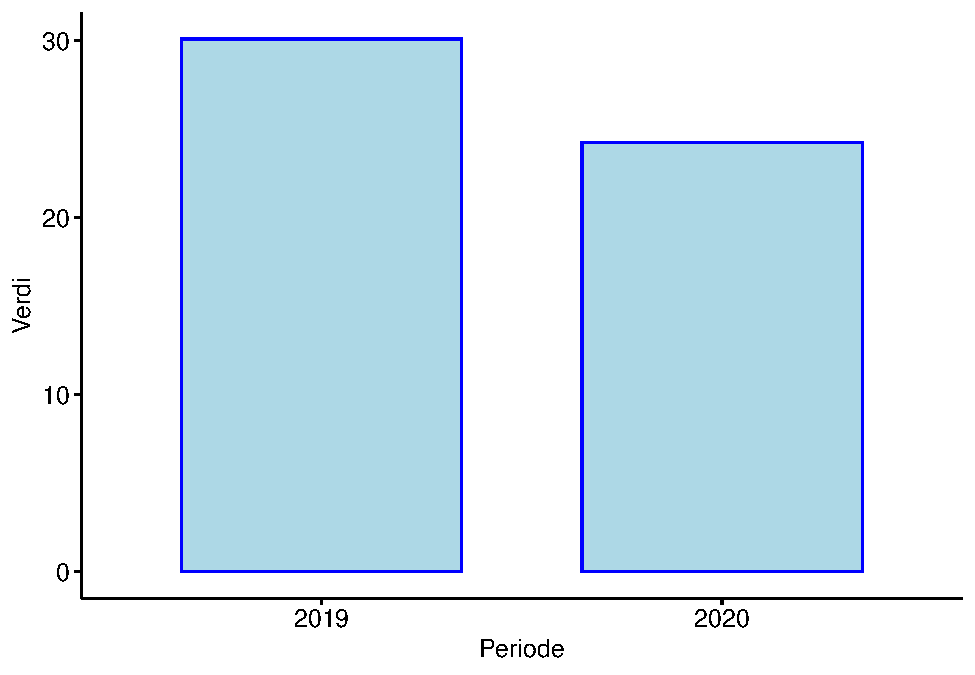
\includegraphics{SPC-book_files/figure-latex/unnamed-chunk-1-1.pdf}

Når man så nærmere på tallene kunne man også se at variasjonen mellom månedene var blitt mindre:

\begin{figure}
\centering
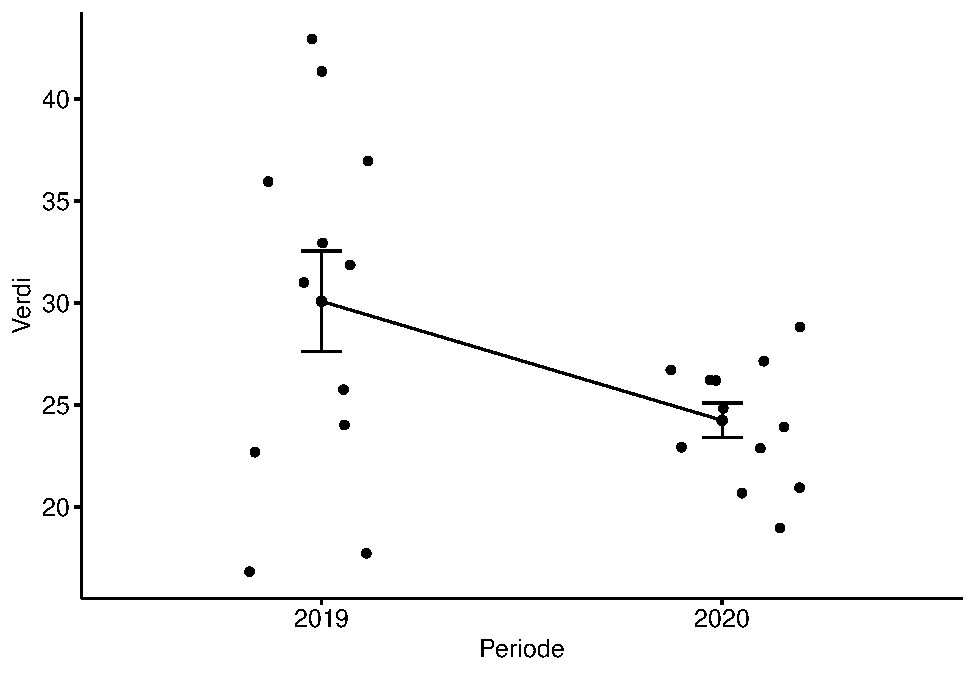
\includegraphics{SPC-book_files/figure-latex/unnamed-chunk-2-1.pdf}
\caption{\label{fig:unnamed-chunk-2}Prosess over 2 år - spredning}
\end{figure}

Dette er nok en kjent tilnærming og konklusjon for mange som har jobbet med eller i organisasjoner som gjør tiltak for å heve kvaliteten. Dessverre er det en tilnærming som i beste fall er unøyaktig, men som i verste fall tåkelegger hva som faktisk skjer og som over tid kan gi dårligere kvalitet. Problemet er at man ikke har sett dataene i et tidsperspektiv. Siden man har data for avvik hver eneste måned vil tidsperspektivet kunne gi helt andre innsikter og konklusjoner.

\begin{figure}
\centering
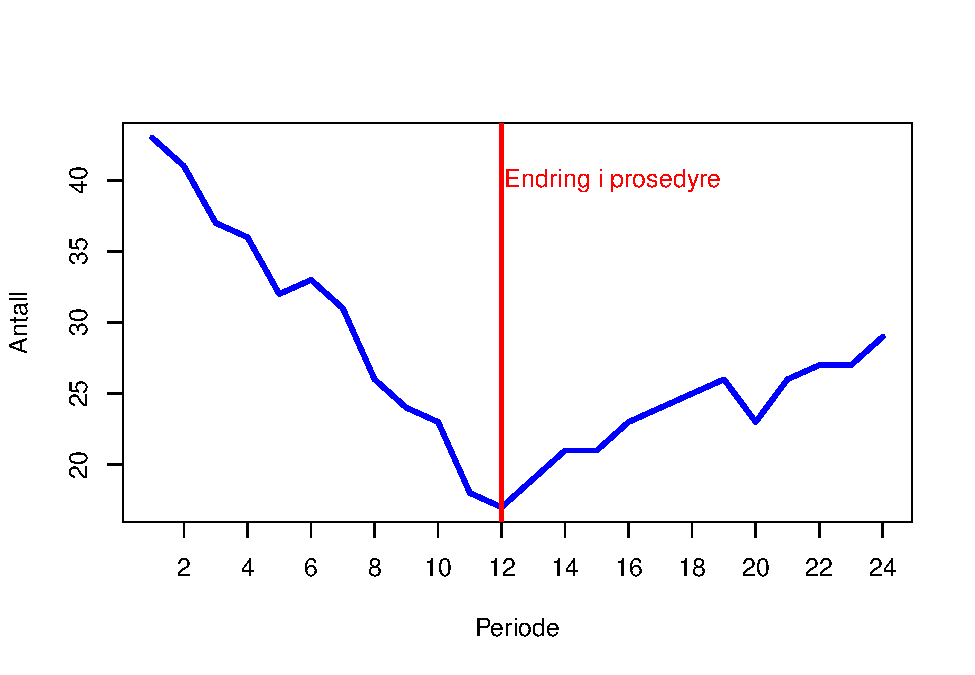
\includegraphics{SPC-book_files/figure-latex/unnamed-chunk-3-1.pdf}
\caption{\label{fig:unnamed-chunk-3}Prosess over 2 år i et tidsperspektiv}
\end{figure}

I diagrammet over har vi plottet inn hver enkelt måned slik at vi får en blå linje som viser utvikling fra måned til måned. Den oransje horisontale streken angir snittet for året (tilsvarende histogrammet lenger opp). Den røde vertikale streken angir årsskiftet og tidspunktet for endring av rutinen. Rent visuelt vil vi nå ha problemer med å konkludere med at endringen av rutinen var en suksess. Vi vil heller tenke at utviklingen gjennom 2019 var veldig positiv, men at endringen ved årsskiftet 2019-2020 har gjort at trenden nå er klart negativ ift at avvikene øker jevnt og trutt igjen. Så kan man spekulere i at det kanskje er innføring av ny rutine som gjør at man igjen får flere avvik og at på litt lengre sikt vil man ha en positiv effekt. Kanskje, det vil vi ikke se før tallene for 2021 begynner å tikke inn. Men det er grunn til å si at dersom man kunne se denne trenden etter 1.kvartal i 2020 hadde man kanskje vurdert tiltak for å endre trenden (eller i det minste gjort en grundig analyse av rutiner og tiltak).

Eksempelet ovenfor er konstruert. Likevel er det grunn til å tro at det ikke er spesielt uvanlig. Mange vil nok kunne kjenne seg igjen i at det jobbes mye med kvalitet i ulike organisasjoner, men at man kanskje ikke har spesielt god kontroll på hva endringer gjør med prosesser, eller at man ikke klarer å fange opp tidsnok at utviklingen går i feil retning. Kanskje har man egentlig lite kontroll på selve prosessen \emph{før} man starter en endringsprosess? Tidsaspektet er med andre ord et viktig aspekt å ha med seg, og helt essensielt i statistisk prosesskontroll som vi hevder bør ha en sentral plass i kvalitetsarbeid.

\hypertarget{hva-er-utgangspunktet-vi-skal-korrigere-fra}{%
\section{Hva er utgangspunktet vi skal korrigere fra?}\label{hva-er-utgangspunktet-vi-skal-korrigere-fra}}

Det kan kanskje virke selvsagt, men en forbedringsprosess vil ha små og tilfeldige sjanser for å lykkes hvis vi ikke kjenner utgangspunktet. Vi vil påstå at mange slike prosesser likevel starter opp med et noe svakt kjennskap til hva startstedet egentlig er. Kvalitetsarbeid -- forbedringsprosesser -- startes som regel fordi man har en oppfatning av at det man leverer ikke er like godt som det man mener man kan og bør levere. Men hva er egentlig problemet? Er det treffsikkerheten (treffer vi målet, det vi sikter mot) eller konsistensen (klarer vi å repetere hendelsen gang etter gang), eller begge deler?\footnote{Illustrasjonen er modifisert fra Montgomery (2020), jfr. Leavengood and Reeb (2015)}

\begin{figure}
\centering
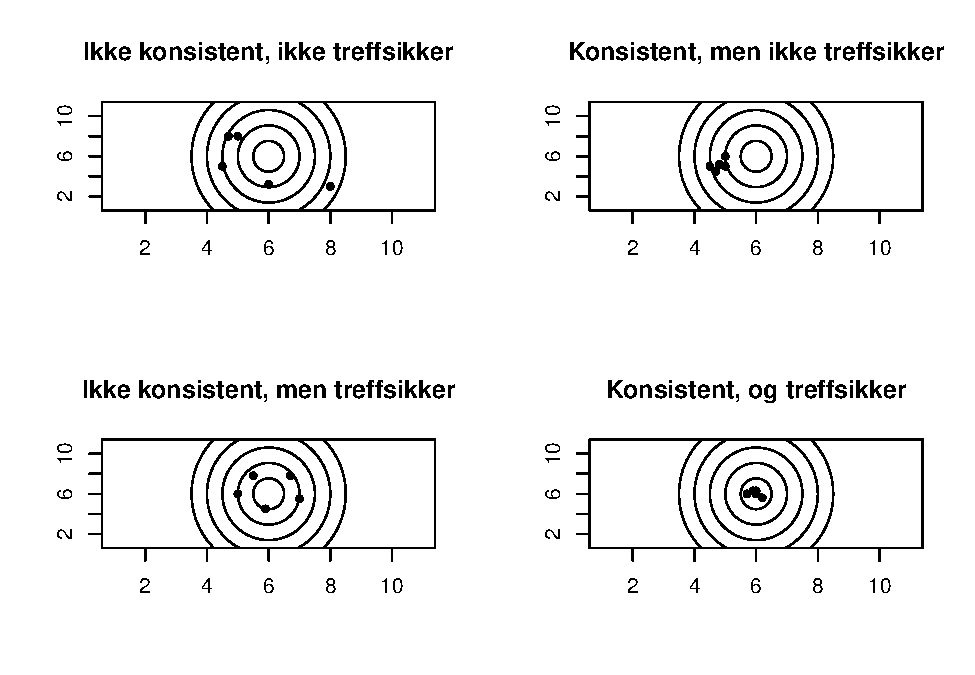
\includegraphics{SPC-book_files/figure-latex/unnamed-chunk-4-1.pdf}
\caption{\label{fig:unnamed-chunk-4}Kjenne til utgangspunktet før vi gjør endringer}
\end{figure}

Det er ganske innlysende at vi vil ha langt større sannsynlighet for å lykkes med en forbedringsprosess om vi har kontroll på hva startsituasjonen er. Her kommer statistisk prosesskontroll inn og kan være et viktig verktøy. Med unntak av den nedre høyre illustrasjonen, der både treffsikkerhet og konsistens er bra, viser alle målskivene en variasjon i hvordan treffene er. Variasjon er et essensielt begrep i statistisk prosesskontroll, og forståelse av variasjon vil følgelig være et viktig tema før vi gir oss i kast med selve analysene. Uten forståelse av prosess og variasjon er det fare for at man forsøker å justere en prosess på feil grunnlag, og i verste fall ville vi kommet bedre ut av endringsprosessen ved å ikke gjøre noe som helst.

\hypertarget{variasjon}{%
\chapter{Variasjon}\label{variasjon}}

Vi skal tilnærme oss begrepet variasjon gjennom å vise til et velkjent eksperiment -- «The Funnel Experiment», eller trakteksperimentet som vi kan kalle det på norsk. Hensikten med trakteksperimentet var å vise at dersom vi ikke forstår variasjon, og introduserer korrigerende tiltak i prosesser som ikke trenger det, står vi i fare for å forverre resultatet (og ofte ha brukt mye tid og ressurser på å justere prosessen i den tro at resultatet vil bli bedre). Eksperimentet illustrerer at mange tiltak i organisasjoner for å «rette på feil» eller «forbedre kvaliteten» ender opp med å ha motsatt virkning.

\begin{figure}
\centering
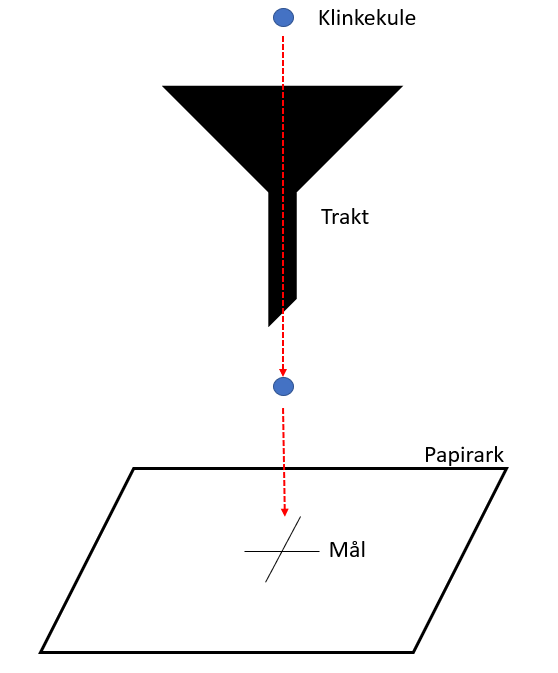
\includegraphics{trakteksp.png}
\caption{Trakteksperimentet - oppsett}
\end{figure}

Trakteksperimentet ble popularisert av Deming (1986) for å beskrive de negative effektene prosessendringer kan ha hvis man ikke forstår årsakene til variasjonen i resultatene (Deming krediterer selv Lloyd Nelson for å ha designiet ekseperimentet, og enkelte kilder omtaler derfor dette som ``the Deming-Nelson funnel experiment'' (Georgantzas and Orsini 2003) . I trakteksperimentet lar vi en klinkekule falle gjennom en trakt vi har sentrert rett over et mål. Der kula treffer arket setter vi et merke. Kula vil aldri treffe nøyaktig på målet og aldri nøyaktig på samme sted fra gang til gang.

La oss si at vi slipper kula gjennom trakta første gang. Trakta er plassert slik at senterlinja gjennom trakta treffer nøyaktig midt i målet. Så slipper vi kula og registerer treffpunktet.

\begin{figure}
\centering
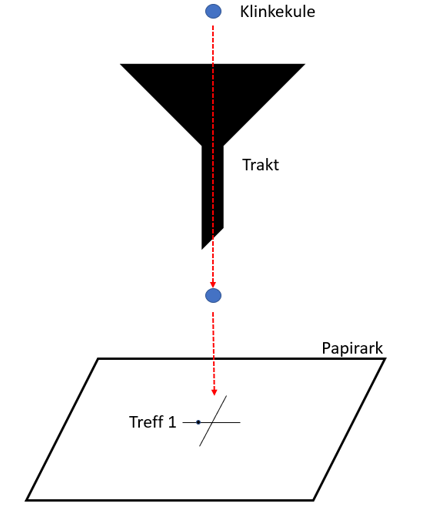
\includegraphics{trakteksp2.png}
\caption{Trakteksperimentet - oppsett}
\end{figure}

Deretter bruker vi 1 av 4 regler for korreksjon for å justere prosessen for å forsøke å få kula til å treffe nærmere målet (se f.eks. (Sparks and Field 2000).

\textbf{Regel 1}
Ingen justering. Selv om kula ikke treffer målet fortsetter vi med neste forsøk uten å gjøre noen justeringer. Vi holder trakta på nøyaktig samme sted.

\textbf{Regel 2}
Trakta justeres etter forrige treffpunkt (treff 1). Hvis kula treffer i z avstand fra målets senterpunkt vil trakta justeres med -z før neste forsøk.

\begin{figure}
\centering
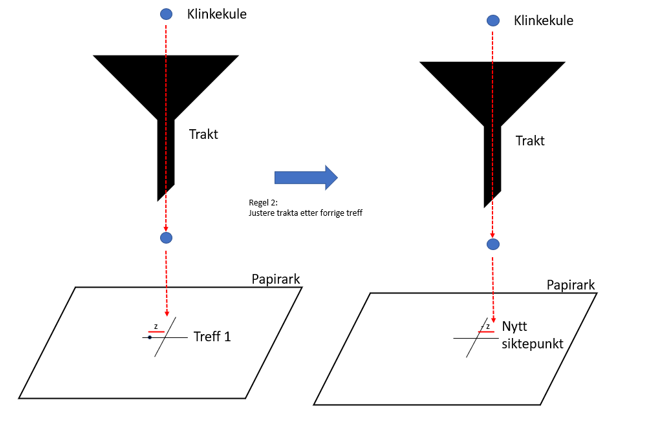
\includegraphics{trakteksp3.png}
\caption{Trakteksperimentet - treff etter første forsøk}
\end{figure}

Så gjentar vi prosessen og korrigerer trakta fra traktas forrige posisjon etter hvert treffpunkt ut fra kulas avstand fra det nye treffpunktet til målets senterpunkt. Justering av trakta skjer etter følgende metode: Plassering av trakta starter i målsenteret (0,0) og justeres deretter slik at ny plassering blir målsenteret blir minus offset (retning og avstand) for forrige kule fra treffpunkt til målsenteret.

Sparks and Field (2000) beskriver regelen slik: ``At drop \emph{i} (\emph{i} = 1,2,3, .) the marble will come to rest at point y\textsubscript{i}, measured from the target. (In other words, y\textsubscript{i} is the error at drop \emph{i}.) Move the funnel the distance -\emph{y}\textsubscript{i} from its last position to aim for the next drop.''

Deming (1986) gir noen eksempler på bruk av regel 2: feedback-mekanismer som reagerer på enkelttilfeller, endring av en policy, rutine e.l. på bakgrunn av (kun) siste kundeundersøkelse, bruke variasjon/avvik til å lage budsjetter og vurdering av en aksje basert på forrige måneds underskudd.

\textbf{Regel 3}
Her registrerer vi treff 1 som i regel 2. Vi flytter trakta til et punkt nøyaktig motsatt av det punktet kula fikk. Vi beregner offset for kula på samme måte som i regel 2 -- retning og avstand fra målsenteret til kulas treffpunkt. Før vi justerer flytter vi imidlertid trakta tilbake til (0,0) og justerer derfra (i motsetning til regel 2 da vi ikke flyttet trakta til (0,0) før vi begynte korreksjonen, men i stedet foretok justeringen fra det punktet trakta befant seg da kula ble sluppet). Her eksemplifiserer Deming (1986) ved å vise til hvordan mer effektiv narkotikabekjempelse fører til høyere priser på narkotika som stimulerer til smugling av mer narkotika, eller en gambler som høyner innsatsen for å dekke forrige tap.

Sparks and Field (2000) beskriver regelen slik: ``At drop \emph{i} the marble comes to rest at point \emph{y}\textsubscript{i} from the target, then for the next drop aim the funnel over the point -\emph{y}\textsubscript{i} from the target.''

\textbf{Regel 4}
Her flytter vi trakta hele tiden til siste treffpunkt og slipper ny kule der. Her viser Deming (1986) til eksempler som den kjente «hviskeleken» der et antall personer sitter i en ring og gjenforteller en historie ved å hviske den til neste person, som igjen hvisker den til neste osv til den kommer til siste person som forteller historien vedkommende nettopp hørte. Historien som til slutt blir fortalt er som regel ganske annerledes enn den opprinnelige. Et annet eksempel kan være produksjon av en gjenstand basert på forrige produserte gjenstands mål.

Sparks and Field (2000) beskriver regelen slik: ``At drop \emph{i} the marble comes to rest at point \emph{y}\textsubscript{i} from the target, then for the next drop aim the funnel over the spot \emph{y}\textsubscript{i} where the marble last came to rest.''

En kort og instruktiv video (Crostic 2015) om gjennomføringen av trakteksperimentet vises kan dere se \href{https://www.youtube.com/watch?v=t5DV69_2VeQ\&ab_channel=MichaelCrostic}{her}.

\hypertarget{simulering-av-trakteksperimentet-i-r}{%
\section{Simulering av trakteksperimentet i R}\label{simulering-av-trakteksperimentet-i-r}}

Vi kan kjøre en simulasjon som viser at resultatet blir suksessivt dårligere etter hvert som vi implementerer reglene. Best resultat kommer fra ingen justering. Dernest gir regel 2 nest best resultat, regel 3 nest dårligst, og til slutt regel 4 det dårligste resultatet. Ved en simulering av 100 repetisjoner kan vi grafisk se hvilket resultat vi får gjennom å anvende de fire ulike reglene. For å kjøre R-koden (jfr vedlegg) må du laste ned disse Excel-filene:

\begin{figure}
\centering
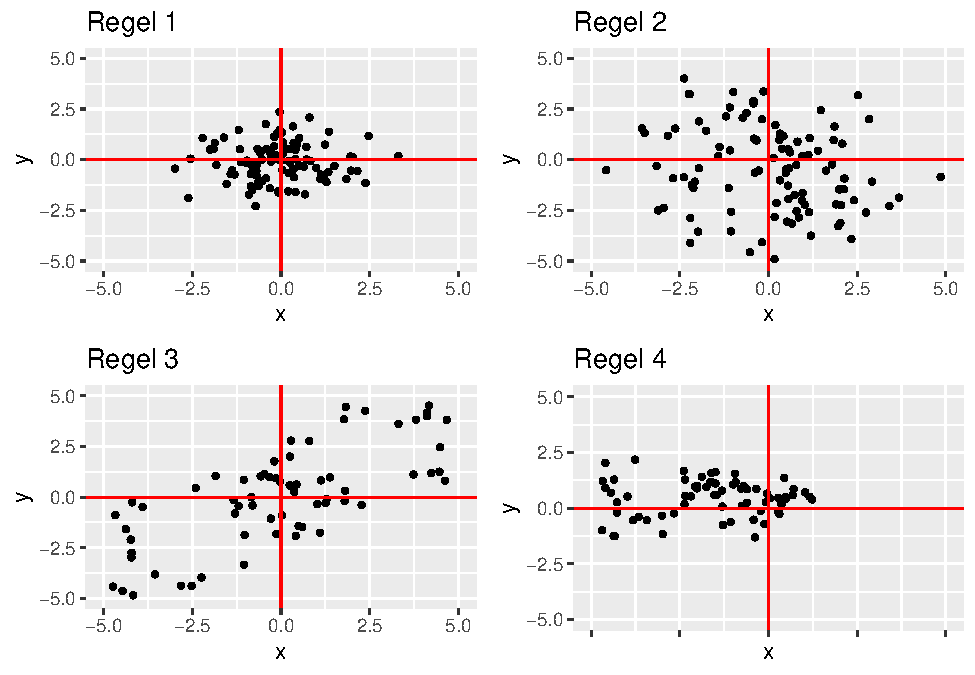
\includegraphics{SPC-book_files/figure-latex/unnamed-chunk-6-1.pdf}
\caption{\label{fig:unnamed-chunk-6}Simulering av trakteksperimentet}
\end{figure}

Det vi kan se er at resultatet etter regel 1 og 2 er sentrert rundt målet, men at regel 2 gir større spredning. Simuleringer viser at regel to gir 40-41 \% større areal i plottet -- eller dobbelt så stor varians (Prevette 2008; SPC for Excel 2006).\footnote{Matematisk sett vil standardavviket ved å legge til n uavhengige tilfeldige observasjoner øke med kvadratroten av n ganger standardavviket for den individuelle observasjonen. Samlet sett dobles variansen, hvilket gir 1,4 ganger høyere standardavvik (siden standardavvik er kvadratroten av variansen, og \(\sqrt{2}\) \(\approx\) 1.4}

Regel 3 vil gi et økende oscillerende mønster. Med en start i nærheten av målet (0,0) vil treffpunktene flytte seg fra side til side stadig lengre vekk fra målet. Mønsteret vil variere, men treffpunktene vil stadig flytte seg lenger unna målet. Hvis vi har et annet førstetreff, vil dette påvirke hvordan mønsteret utvikler seg.

For å kjøre R-koden for alternativt førstetreffpunkt må du laste ned denne Excel-fila:

\begin{figure}
\centering
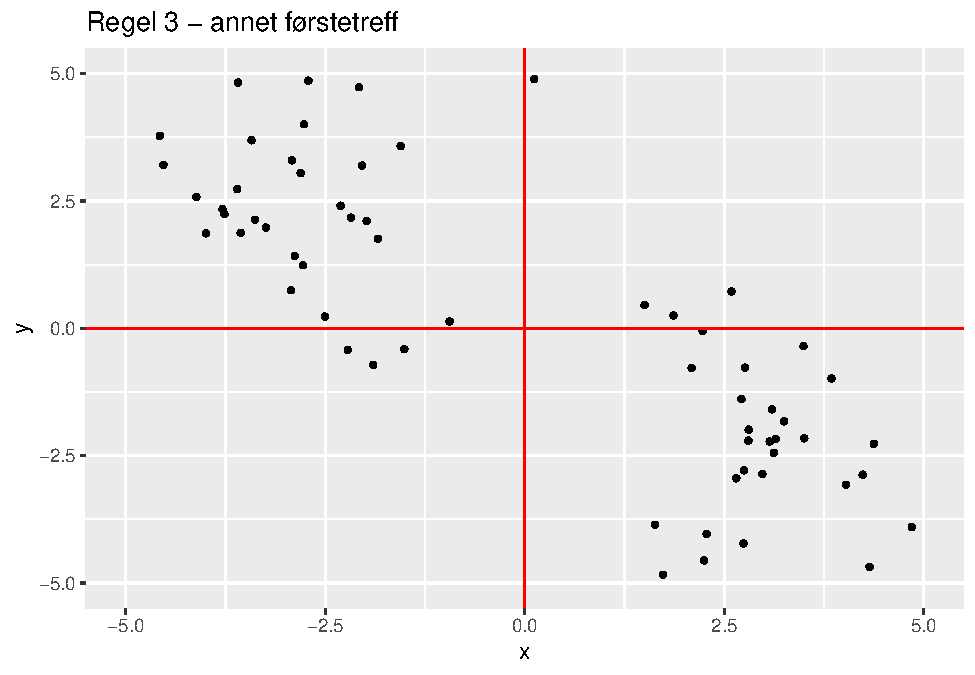
\includegraphics{SPC-book_files/figure-latex/unnamed-chunk-8-1.pdf}
\caption{\label{fig:unnamed-chunk-8}Regel 3 - annet førstetreff}
\end{figure}

Regel 4 vil alltid medføre at treffpunktet vil bevege seg lenger og lenger unna målet. Med et annet førstetreff vil mønsteret se annerledes ut.

For å kjøre R-koden for alternativt førstetreffpunkt må du laste ned denne Excel-fila:

\begin{figure}
\centering
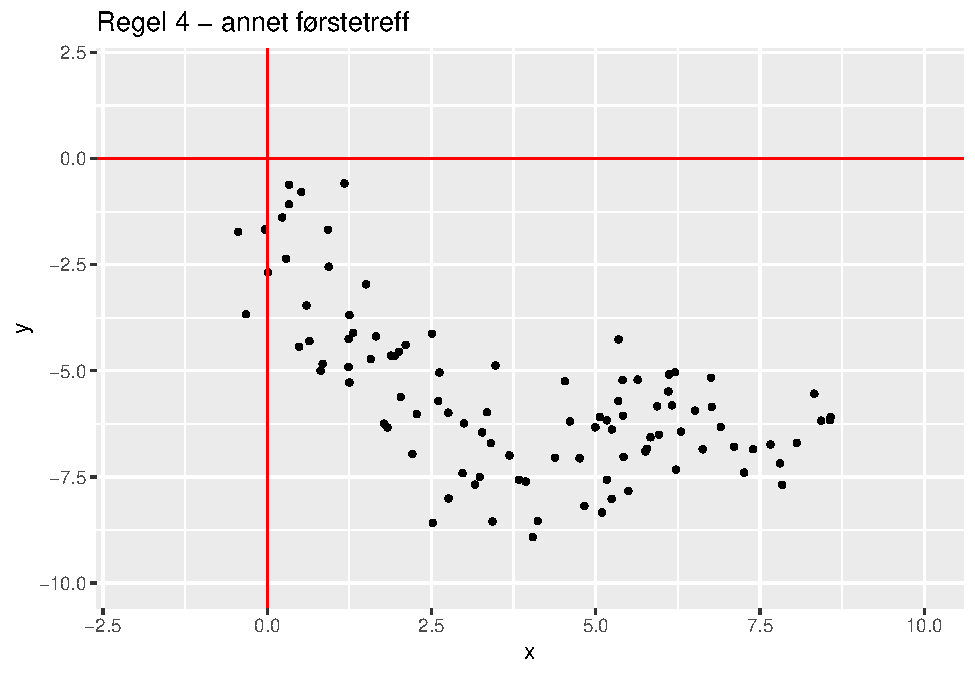
\includegraphics{SPC-book_files/figure-latex/unnamed-chunk-10-1.pdf}
\caption{\label{fig:unnamed-chunk-10}Regel 4 - annet førstetreff}
\end{figure}

Eksperimentet, som altså som regel refereres til som Deming's trakteksperiment (``Funnel experiment''), men refereres også som Nelsons trakteksperiment (se f.eks. Alwan (1991)) illustrerer en viktig erkjennelse i alt kvalitetsarbeid: hvis man ikke vet hva man driver med kan man i beste hensikt fort ende opp med å korrigere en prosess ``ut i evigheten'' vekk fra målet. Dessverre er det grunn til å tro at mange forbedringsprosesser ender opp på denne måten.

Eksperimentet illustrerer videre en viktig observasjon: alle prosesser har variasjon. Hvis vi tenker over det, vil vi lett finne eksempler fra dagliglivet. Vi sover et antall timer og minutter sammenhengende søvn hver natt som ikke vil være det samme fra natt til natt, men som regel ligge innenfor et visst intervall. Vi har en hvilepuls når vi våkner om morgenen. Måler vi den vil vi se variasjon. Vi kjører til jobben, og tidsbruken vil variere fra dag til dag. Vi tar en treningstur på kvelden. Selv om vi løper samme runde med samme utstyr vil tiden vi bruker variere. Eller strømregningen vi betaler hver måned. Hva med kostnader for en sykehusavdeling? Antall overtidstimer i en organisasjon? Mengde materialer i en bestemt produksjonslinje? Alle de ovennevnte er prosesser som har en variasjon.

Variasjon kan være normal eller unormal. Med normal variasjon mener vi variasjon som ikke kan tilskrives en spesiell årsak (ofte omtalt som ``common cause variation'' og opprinnelig av Shewhart som ``assignable cause''). Tilsvarende kan unormal variasjon tilskrives en eller flere spesifikke årsaker (``special cause variation,'' av Shewhart benevnt som ``chance cause''). Normal variasjon skyldes fenomen som alltid er til stede i en prosess, og kan dermed ikke endres uten at man endrer selve prosessen. Det betyr også at normal variasjon er det som gjør prosesser forutsigbare i større eller mindre grad.

Unormal variasjon på sin side skyldes en (eller flere) ikke-tilfeldige påvirkninger som ikke vanligvis er til stede i prosessen. Dette gjør prosessen uforutsigbar. Problemene oppstår når man ikke skiller mellom de to typene variasjon, og jager etter spesielle årsaker til variasjon når det i realiteten kun er normal variasjon man observerer. Da jager man etter å løse problemer uten å forstå årsakene.

La oss se på dataene fra trakteksperimentet igjen, og denne gangen skal vi plotte datapunktene på en måte som gjør at vi ser hvordan treffpunktene varierer ved at vi plotter på en tidsakse (første forsøk til venstre, siste til høyre på x-aksen). Vi kan først se på treffpunkter for x- og y-verdi for hhv regel 1 og 2.

\begin{figure}
\centering
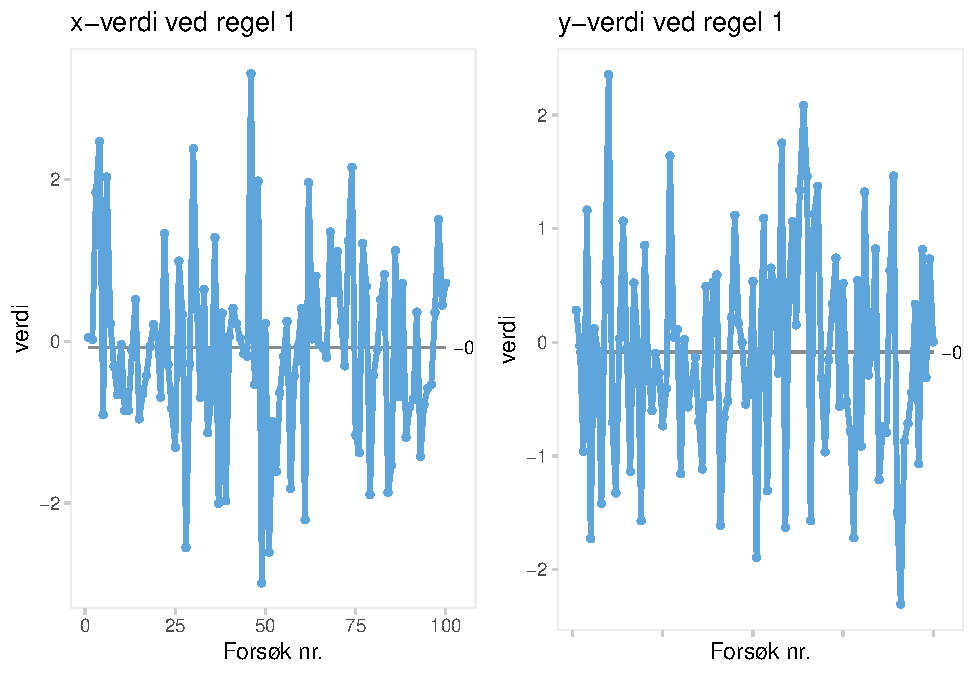
\includegraphics{SPC-book_files/figure-latex/unnamed-chunk-11-1.pdf}
\caption{\label{fig:unnamed-chunk-11}x- og y-verdier for regel 1}
\end{figure}

\begin{figure}
\centering
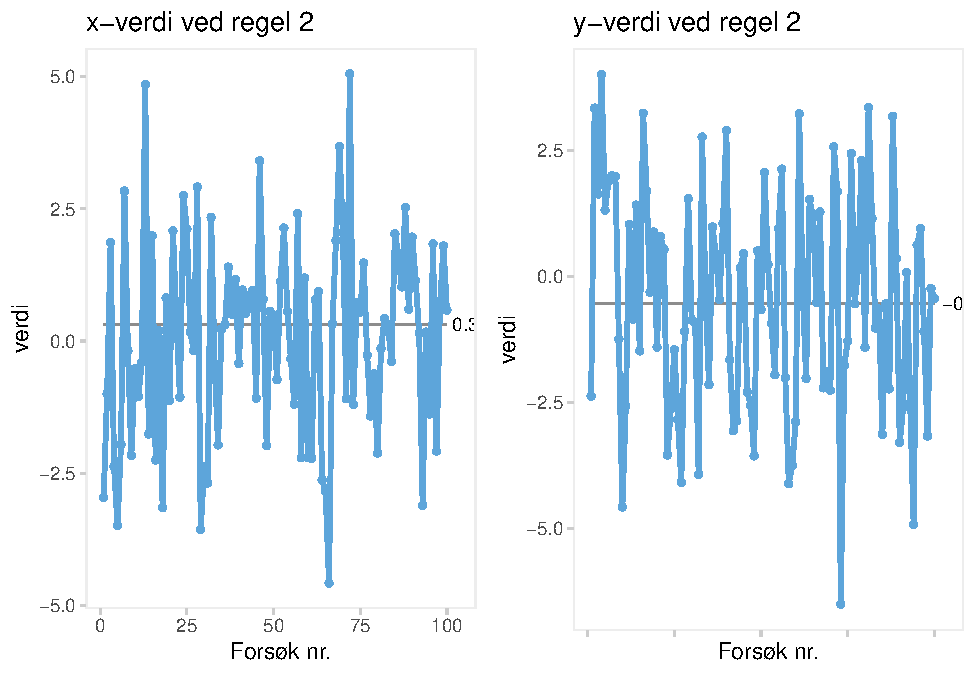
\includegraphics{SPC-book_files/figure-latex/unnamed-chunk-12-1.pdf}
\caption{\label{fig:unnamed-chunk-12}x- og y-verdier for regel 2}
\end{figure}

Det vi kan se er:
* Mønstrene likner på hverandre i hvordan de varierer
* De varierer like mer eller mindre like mye over og under x = 0 og y = 0. En absolutt perfekt prosess ville gitt null avvik fra 0,0 for hvert forsøk. Dette tyder på at variasjonen er sentrert rundt målpunktet.
* Vi kan se at avviket er noe større for regel 2, spesielt på x-verdiene. Dette er iht forventning siden vi vet at variansen er dobbelt så stor for regel 2 som for regel 1.
* Vi ser også at gjennomsnittet (markert med horisontal linje) er nærme 0 for både x- og y-verdi for regel 1, mens den er noe mer avvikende for begge verdiene for regel 2.

Hvis vi ser på x- og y-verdiene for regel 3 får vi et helt annet bilde.

\begin{figure}
\centering
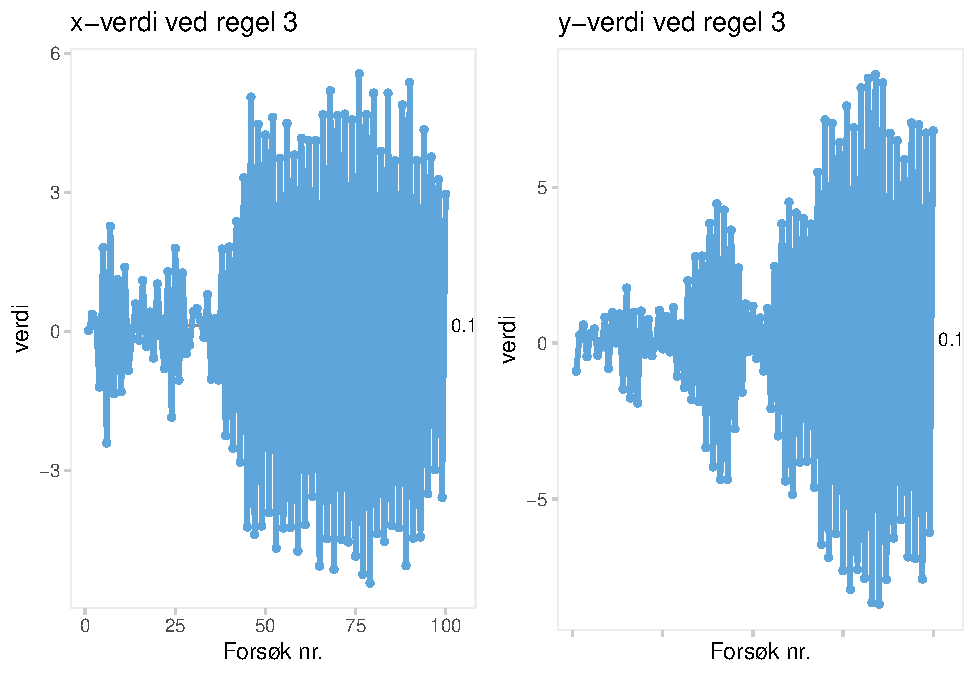
\includegraphics{SPC-book_files/figure-latex/unnamed-chunk-13-1.pdf}
\caption{\label{fig:unnamed-chunk-13}x- og y-verdier for regel 3}
\end{figure}

Vi ser at vi får en økende oscillerende trend. Samtidig ser vi at treffene er sentrert rundt 0, men at treffpunktene i stadig økende grad fjerner seg fra 0. Mønsteret er også veldig likt for x-verdi og y-verdi.

Til slutt kan vi se på regel 4.

\begin{figure}
\centering
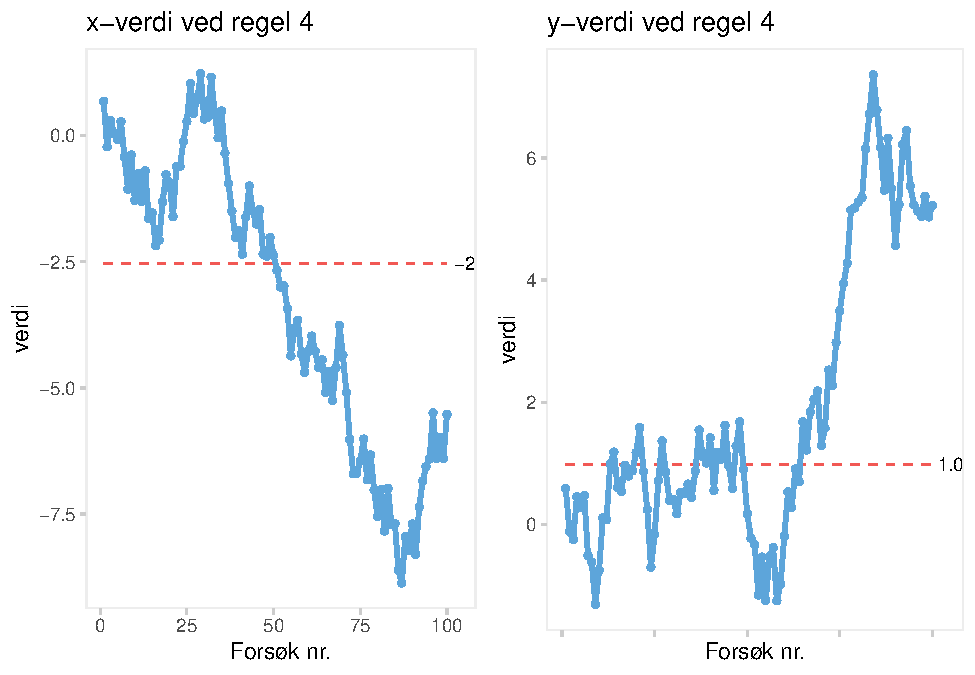
\includegraphics{SPC-book_files/figure-latex/unnamed-chunk-14-1.pdf}
\caption{\label{fig:unnamed-chunk-14}x- og y-verdier for regel 4}
\end{figure}

Det vi kan legge merke til er at begge verdiene starter nærme 0, men at de -- som forventet -- etter hvert fjerner seg i en trend vekk fra 0. Hadde man kjørt 1000 eller 10000 forsøk ville denne trenden vært enda tydeligere.

Dette leder oss til to begrep som er vesentlige i kvalitetsarbeid. Er prosessen kontrollert («in control») eller er den ukontrollert («out of control»)? Prosesser med kun normal variasjon er kontrollerte prosesser, mens prosesser med unormal variasjon er ukontrollerte prosesser. I en kontrollert, stabil prosess er årsakene til variasjon i ytelse/resultater konstant over tid. Dette betyr altså ikke at det ikke er variasjon i ytelse/resultater/kvalitet, at variasjonen er liten eller at kvaliteten er god nok.

Under har vi simulert to team som jobber parallelt med å produsere samme produkt, samme maskiner, med samme råmaterialer. Vi skal ikke gå nærmere inn på variasjon o.l., men kan kort konstatere at begge prosessene er i kontroll. Vi kommer tilbake til kontrollgrenser om kort tid, men kort fortalt må alle punkter ligge innenfor kontrollgrensene for at prosessen skal være i kontroll. For å kjøre R-koden må du laste ned følgende fil:

\begin{figure}
\centering
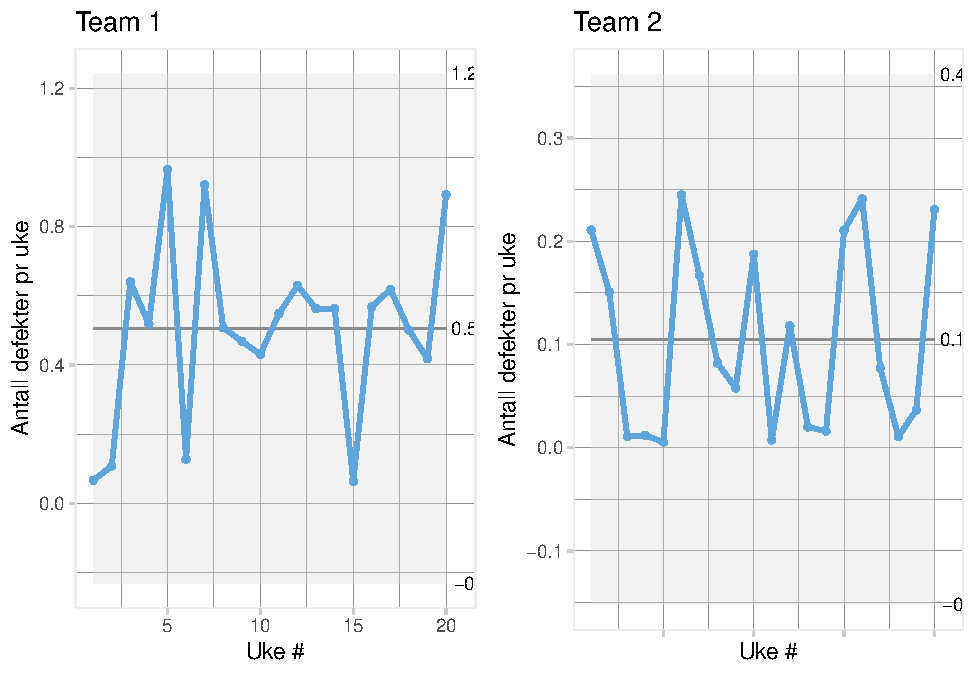
\includegraphics{SPC-book_files/figure-latex/unnamed-chunk-16-1.pdf}
\caption{\label{fig:unnamed-chunk-16}To teams kontrolldiagrammer}
\end{figure}

Imidlertid ser vi at Team 1's prosess har større variasjon enn team 2's (selv om de ser like ut må vi ta hensyn til at y-aksene er ulike (legg merke til verdiene 1,2 og 0,4 som viser den øvre kontrollgrensen. Vi ser også at gjennomsnittet ligger på hhv 0.5 og 0.1 for team 1 og 2. Dersom vi arrangerer plottene med samme skala på y-aksen ser vi en klar forskjell mellom de to teamene:

\begin{figure}
\centering
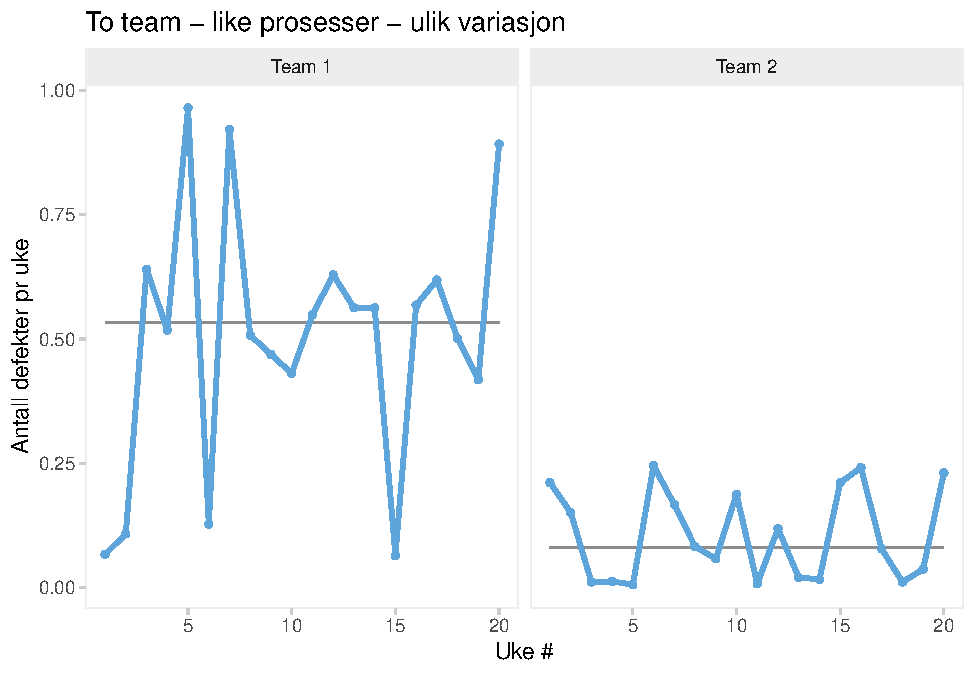
\includegraphics{SPC-book_files/figure-latex/unnamed-chunk-17-1.pdf}
\caption{\label{fig:unnamed-chunk-17}To teams - like prosesser - ulik variasjon}
\end{figure}

Vi trenger altså ikke være fornøyde med en stabil og kontrollert prosess. Det betyr bare at variasjonen er forutsigbar innenfor statistisk etablerte grenser (Nolan and Provost 1990), og at ytelsen fra prosessen ikke vil endre seg vesentlig med mindre man endrer selve prosessen.Begge prosessene over er kontrollerte, men det kan virke åpenbart at man vil se nærmere på hvorfor det ene teamet skiller seg veldig fra det andre.

Arbeidet med statistisk prosesskontroll handler i hovedsak om dette: Forstå prosessen og forstå variasjonen. Trakteksperimentet viser oss også at korreksjon av prosesser kan lede oss lenger og lenger fra målet om vi ikke forstår variasjon og kontrollerte vs.~ukontrollerte prosesser. Deming omtaler dette som «tampering with the process» - tukling med prosessen («If it ain't broken, don't fix it»). I jakten på små forbedringer er det fristende å gjøre små justeringer ofte. Det kan være en smart strategi, men det kan også gi motsatt effekt: variasjonen i resultatene blir bare større og større (i takt med desperasjonen etter ønskede forbedringer). Dette vil vi kalle for over-kontrollering av prosesser.

Erkjennelsen av variasjon i prosesser og om prosesser i kontrollert eller ukontrollert har klare ledelsesmessige utfordringer og konsekvenser. Nolan and Provost (1990, s.3, figur 1) illustrerer to ulike tilnærminger til variasjon:

\providecommand{\docline}[3]{\noalign{\global\setlength{\arrayrulewidth}{#1}}\arrayrulecolor[HTML]{#2}\cline{#3}}

\setlength{\tabcolsep}{2pt}

\renewcommand*{\arraystretch}{1.5}

\begin{longtable}[c]{ccc}



\hhline{>{\arrayrulecolor[HTML]{666666}\global\arrayrulewidth=2pt}->{\arrayrulecolor[HTML]{666666}\global\arrayrulewidth=2pt}->{\arrayrulecolor[HTML]{666666}\global\arrayrulewidth=2pt}-}

\multicolumn{1}{!{\color[HTML]{000000}\vrule width 0pt}>{}l}{\fontsize{11}{11}\selectfont{\textcolor[HTML]{000000}{Områder}}} & \multicolumn{1}{!{\color[HTML]{000000}\vrule width 0pt}>{}l}{\fontsize{11}{11}\selectfont{\textcolor[HTML]{000000}{Variasjon1}}} & \multicolumn{1}{!{\color[HTML]{000000}\vrule width 0pt}>{}l!{\color[HTML]{000000}\vrule width 0pt}}{\fontsize{11}{11}\selectfont{\textcolor[HTML]{000000}{Variasjon2}}} \\

\hhline{>{\arrayrulecolor[HTML]{666666}\global\arrayrulewidth=2pt}->{\arrayrulecolor[HTML]{666666}\global\arrayrulewidth=2pt}->{\arrayrulecolor[HTML]{666666}\global\arrayrulewidth=2pt}-}

\endfirsthead

\hhline{>{\arrayrulecolor[HTML]{666666}\global\arrayrulewidth=2pt}->{\arrayrulecolor[HTML]{666666}\global\arrayrulewidth=2pt}->{\arrayrulecolor[HTML]{666666}\global\arrayrulewidth=2pt}-}

\multicolumn{1}{!{\color[HTML]{000000}\vrule width 0pt}>{}l}{\fontsize{11}{11}\selectfont{\textcolor[HTML]{000000}{Områder}}} & \multicolumn{1}{!{\color[HTML]{000000}\vrule width 0pt}>{}l}{\fontsize{11}{11}\selectfont{\textcolor[HTML]{000000}{Variasjon1}}} & \multicolumn{1}{!{\color[HTML]{000000}\vrule width 0pt}>{}l!{\color[HTML]{000000}\vrule width 0pt}}{\fontsize{11}{11}\selectfont{\textcolor[HTML]{000000}{Variasjon2}}} \\

\hhline{>{\arrayrulecolor[HTML]{666666}\global\arrayrulewidth=2pt}->{\arrayrulecolor[HTML]{666666}\global\arrayrulewidth=2pt}->{\arrayrulecolor[HTML]{666666}\global\arrayrulewidth=2pt}-}\endhead



\multicolumn{1}{!{\color[HTML]{000000}\vrule width 0pt}>{}l}{\fontsize{11}{11}\selectfont{\textcolor[HTML]{000000}{}}} & \multicolumn{1}{!{\color[HTML]{000000}\vrule width 0pt}>{}l}{\fontsize{11}{11}\selectfont{\textcolor[HTML]{000000}{Som\ indikator\ på\ god\ eller\ dårlig\ ytelse}}} & \multicolumn{1}{!{\color[HTML]{000000}\vrule width 0pt}>{}l!{\color[HTML]{000000}\vrule width 0pt}}{\fontsize{11}{11}\selectfont{\textcolor[HTML]{000000}{Som\ resultat\ av\ normal\ eller\ unormal\ variasjon}}} \\





\multicolumn{1}{!{\color[HTML]{000000}\vrule width 0pt}>{}l}{\fontsize{11}{11}\selectfont{\textcolor[HTML]{000000}{Fokus}}} & \multicolumn{1}{!{\color[HTML]{000000}\vrule width 0pt}>{}l}{\fontsize{11}{11}\selectfont{\textcolor[HTML]{000000}{Resultat\ av\ prosessen\ (produkt,\ tjeneste)}}} & \multicolumn{1}{!{\color[HTML]{000000}\vrule width 0pt}>{}l!{\color[HTML]{000000}\vrule width 0pt}}{\fontsize{11}{11}\selectfont{\textcolor[HTML]{000000}{Årsaker\ til\ variasjon\ i\ prosessen}}} \\





\multicolumn{1}{!{\color[HTML]{000000}\vrule width 0pt}>{}l}{\fontsize{11}{11}\selectfont{\textcolor[HTML]{000000}{Mål}}} & \multicolumn{1}{!{\color[HTML]{000000}\vrule width 0pt}>{}l}{\fontsize{11}{11}\selectfont{\textcolor[HTML]{000000}{Klassifisere\ resultat\ som\ akseptabelt\ eller\ ikke}}} & \multicolumn{1}{!{\color[HTML]{000000}\vrule width 0pt}>{}l!{\color[HTML]{000000}\vrule width 0pt}}{\fontsize{11}{11}\selectfont{\textcolor[HTML]{000000}{Gi\ grunnlag\ for\ endring\ av\ prosess}}} \\





\multicolumn{1}{!{\color[HTML]{000000}\vrule width 0pt}>{}l}{\fontsize{11}{11}\selectfont{\textcolor[HTML]{000000}{Grunnlag}}} & \multicolumn{1}{!{\color[HTML]{000000}\vrule width 0pt}>{}l}{\fontsize{11}{11}\selectfont{\textcolor[HTML]{000000}{Hva\ kunden\ ønsker\ eller\ trenger}}} & \multicolumn{1}{!{\color[HTML]{000000}\vrule width 0pt}>{}l!{\color[HTML]{000000}\vrule width 0pt}}{\fontsize{11}{11}\selectfont{\textcolor[HTML]{000000}{Hva\ prosessen\ faktisk\ gir}}} \\





\multicolumn{1}{!{\color[HTML]{000000}\vrule width 0pt}>{}l}{\fontsize{11}{11}\selectfont{\textcolor[HTML]{000000}{Metoder}}} & \multicolumn{1}{!{\color[HTML]{000000}\vrule width 0pt}>{}l}{\fontsize{11}{11}\selectfont{\textcolor[HTML]{000000}{Metoder\quad Spesifikasjoner,\ budsjetter,\ prognoser,\ numeriske\ mål,\ verktøy\ for\ å\ måle\ ytelse}}} & \multicolumn{1}{!{\color[HTML]{000000}\vrule width 0pt}>{}l!{\color[HTML]{000000}\vrule width 0pt}}{\fontsize{11}{11}\selectfont{\textcolor[HTML]{000000}{Kontrolldiagram}}} \\

\hhline{>{\arrayrulecolor[HTML]{666666}\global\arrayrulewidth=2pt}->{\arrayrulecolor[HTML]{666666}\global\arrayrulewidth=2pt}->{\arrayrulecolor[HTML]{666666}\global\arrayrulewidth=2pt}-}



\end{longtable}

En klar svakhet ved den første tilnærmingen -- som indikator på god eller dårlig ytelse -- er at det tilbyr lite informasjon og grunnlag for forbedring. Likevel, mange vil nok kjenne seg igjen i fokus, mål, grunnlag og metoder i denne tilnærmingen.

En kjerne i ledelse i organisasjoner må derfor være å kunne avgjøre om variasjonen fra ulike prosesser er normal eller unormal, og om svingninger indikerer en trend eller en tilfeldig variasjon som følger mønstre vi har sett tidligere. Nolan and Provost (1990) peker på mulige konsekvenser i organisasjoner av å trekke feilslutninger om variasjon: Skylden for problemer legges på ansatte som er utenfor deres kontroll, kostnader til nytt utstyr som ikke er nødvendig, bortkastet tidsbruk for å lete etter forklaringer på en antatt trend når ingenting egentlig har endret seg og gjennomføre tiltak når det ville ha vært bedre å ikke gjøre noe.

\begin{figure}
\centering
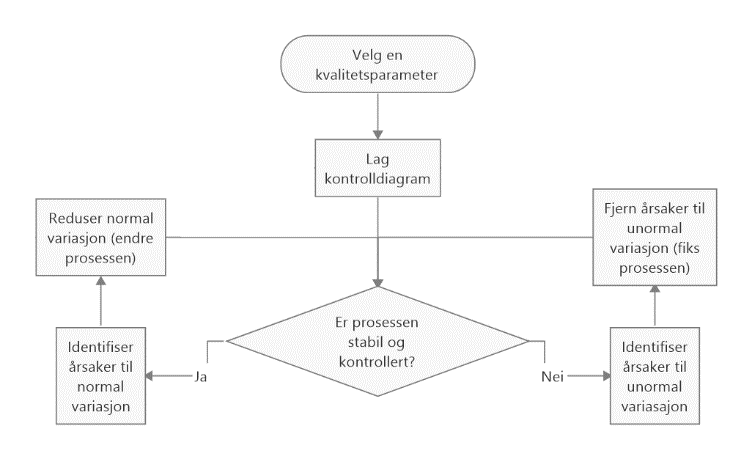
\includegraphics{nolan_provost.png}
\caption{modifisert fra Nolan \& Provost, 1990, s.9, figur 2}
\end{figure}

Deming (1986) peker på at det store rommet for forbedring (94 \%) ligger i endring av prosessen -- altså i å jobbe med den normale variasjonen (gitt at prosessen er stabil). Kun 6 \% av potensialet ligger i å fikse spesielle ting -- unormal variasjon -- som skjer. Her ser vi en veldig klar kobling til ledelsesaspektet og ledelsesansvaret som ligger i å realisere potensialet for forbedringer.

\hypertarget{datatyper-og-datafordelinger}{%
\chapter{Datatyper og datafordelinger}\label{datatyper-og-datafordelinger}}

Ift statistisk prosesskontroll er det formålstjenlig å snakke om tre hovedtyper data: måledata, telledata og sjeldne hendelser. Måledata er kontinuerlige data -- det vil si de kan måles på en skala som høyde, vekt og tid. Her kan en observasjon/et datapunkt innta en hvilken som helst verdi innenfor et gitt spenn. Høyden på en person kan være 178,34227809 cm eller 178,34227808 cm.

Telledata et kategoriske (også ofte omtalt som diskrete) data -- det vil si et datapunkt (en observasjon) kan puttes inn i en klar kategori, som f.eks. antall avvik, antall hendelser, ja/nei, terningkast. Diskrete data har et begrenset antall mulige verdier som er gjensidig utelukkende. Et terningkast med en vanlig terning kan ikke både være 3 og 4 samtidig, en lysbryter kan ikke være av og på samtidig. Et terningkast kan heller ikke være 1,43. Med tanke på datafordeling er både binomial-, Poissonfordeling og geomterisk fordeling diskrete fordelinger, mens normalfordeling og eksponensiell fordeling vil være kontinuerlig (se f.eks. Ugarte, Militino, and Arnholt (2016)).

Når det gjelder sjeldne hendelser kan de være både telledata og måledata. For eksempel vil antall dager mellom en hendelse være en diskret data, mens tid kan måles og vil være kontinuerlige data. Det er spesielle utfordringer med det vi kaller sjeldne hendelser finnes det også egne måter å håndtere dette på i statistisk prosesskontroll, noe vi vil komme tilbake til. For sjeldne henselser vil både geometrisk og eksponensiell fordeling være relevant. Det finnes en god del flere fordelinger enn disse som nå er nevnt, men som Benneyan (1998) viser er normal-, binomial- og Poissonfordeling de tre vesentligste. For en god oversikt over flere fordelinger, se f.eks. Mun (2008).

Hvorfor fokus på fordelinger?

Fordelingene -- normalfordeling, binomialfordeling, Poissionfordeling, geometrisk fordeling og eksponensiell fordeling -- beskriver ulike fordelinger ut fra hvordan dataene ser ut. Vi bruker forventningene/sannsynlighetene for ulike verdier i statistisk prosesskontroll til å vurdere om en verdi av en observasjon eller måling er innenfor eller utenfor det vi vil kalle normal variasjon (jfr kapittelet om variasjon). Siden dataene kan være av ulik type -- diskret eller kontinuerlig, binomial/ikke binomial osv -- bruker vi ulike utregningsmetoder og diagrammer i statistisk prosesskontroll for å få et riktig resultat. Det finnes et antall ulike diagrammer å velge mellom i statistisk prosesskontroll. For å gjøre valget sikrere og lettere kan man bruke følgende flytskjema for å orientere seg:

\begin{figure}
\centering
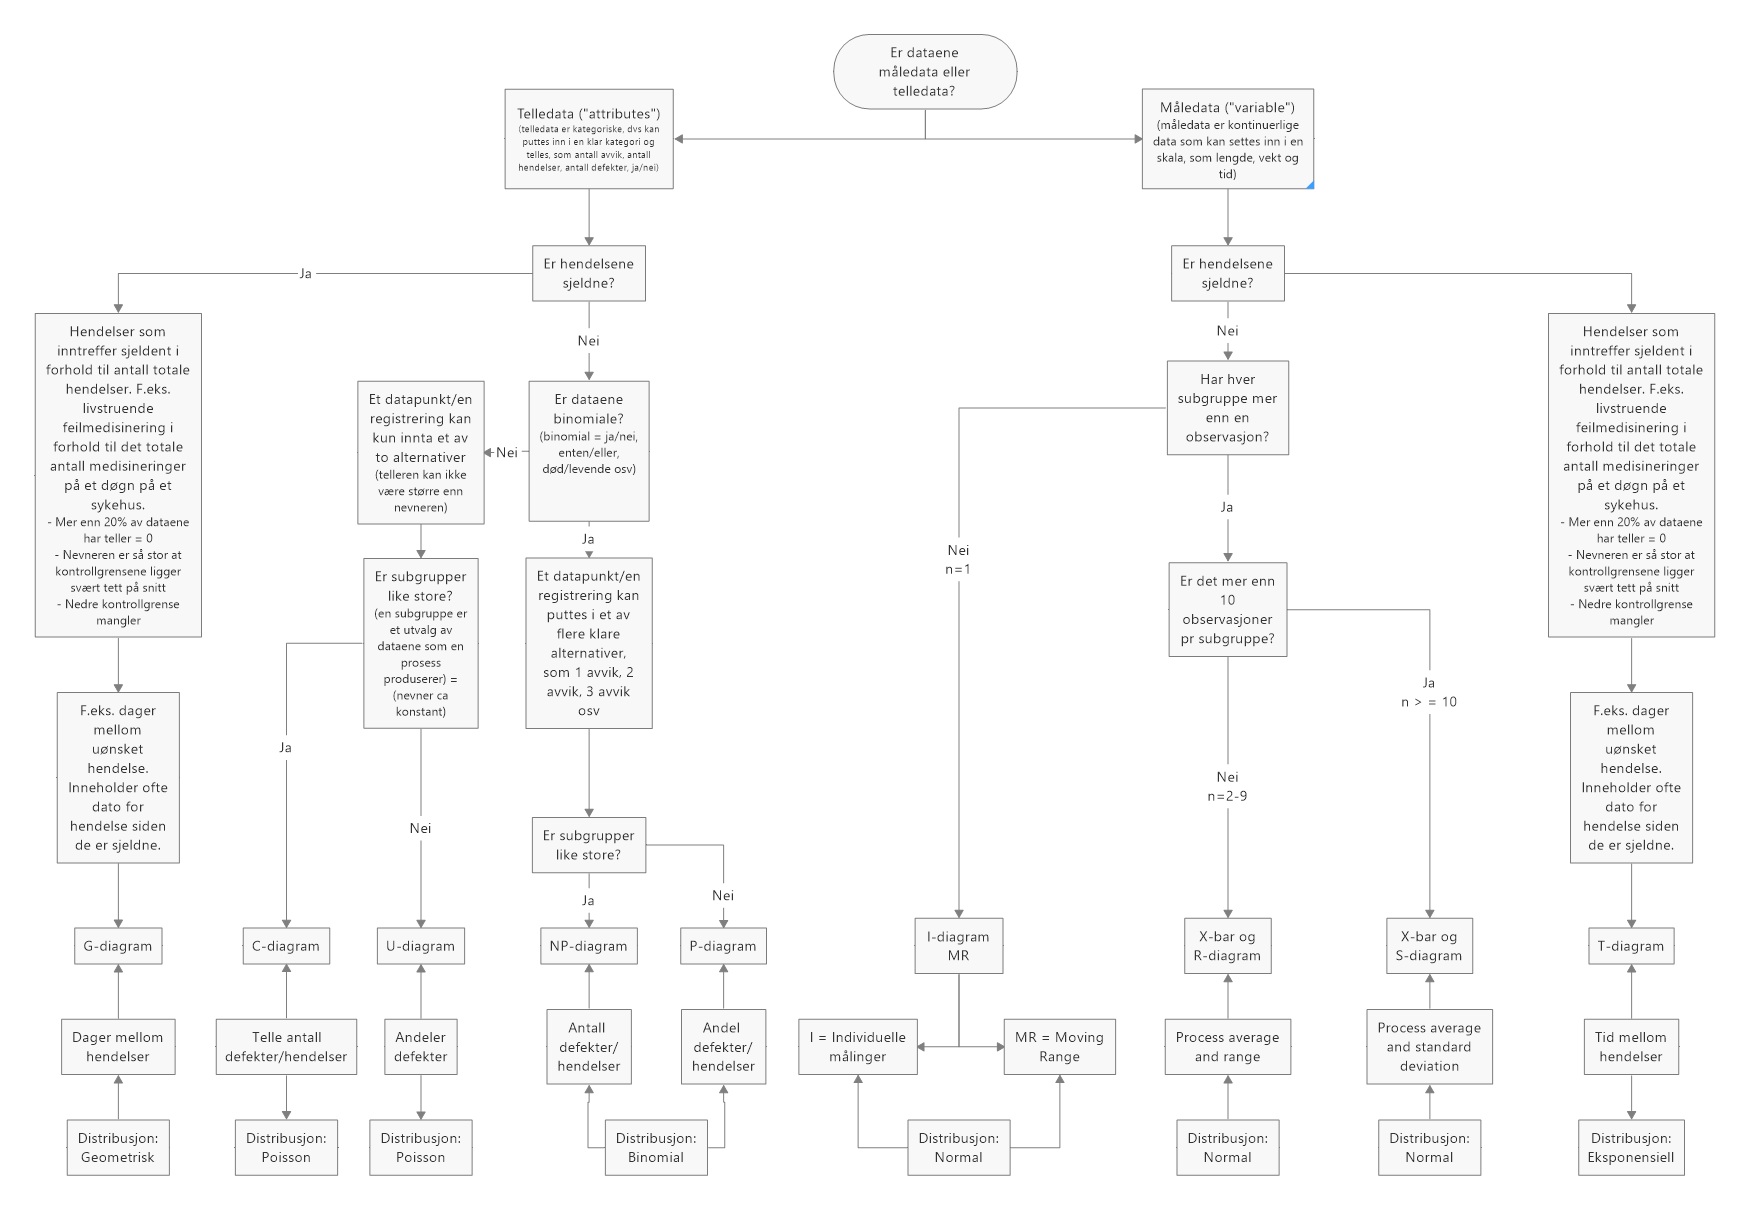
\includegraphics{Flytdiagram_valg.png}
\caption{Flytdiagram for valg av analyse}
\end{figure}

Senere kommer vi tilbake til de ulike diagrammene gjennom praktiske eksempler. Før vi kommer dit vil vi gå gjennom de sentrale datafordelingstypene.

\hypertarget{normalfordeling}{%
\section{Normalfordeling}\label{normalfordeling}}

Når vi snakker om distribusjonen av et datasett tenker vi på hvordan dataene vi har samlet inn fordeler seg i forhold til hverandre etter gitte egenskaper. Vi kan for eksempel ha målt høyden på 100 mennesker. Disse dataene utgjør da en observert fordeling som vi kan sette inn i et diagram for å visualisere hvordan datasettet ser ut.

\begin{figure}
\centering
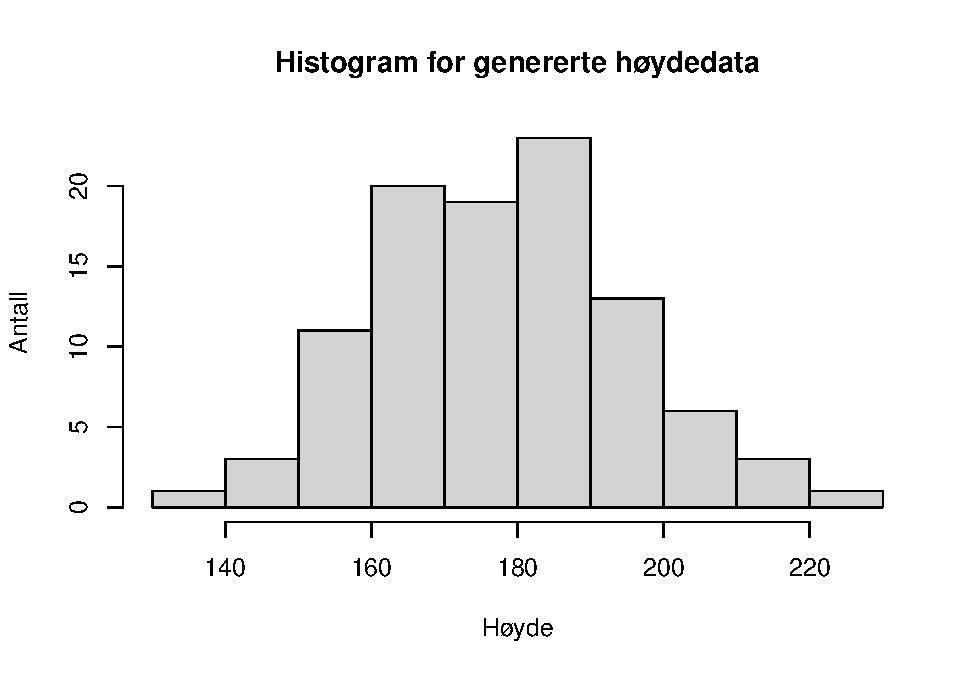
\includegraphics{SPC-book_files/figure-latex/unnamed-chunk-19-1.pdf}
\caption{\label{fig:unnamed-chunk-19}Høydefordeling for 100 tilfeldige menn, genererte data}
\end{figure}

Hvis vi samler inn høydedata for 100 andre tilfeldig menn kan fordelingen se slik ut:

\begin{figure}
\centering
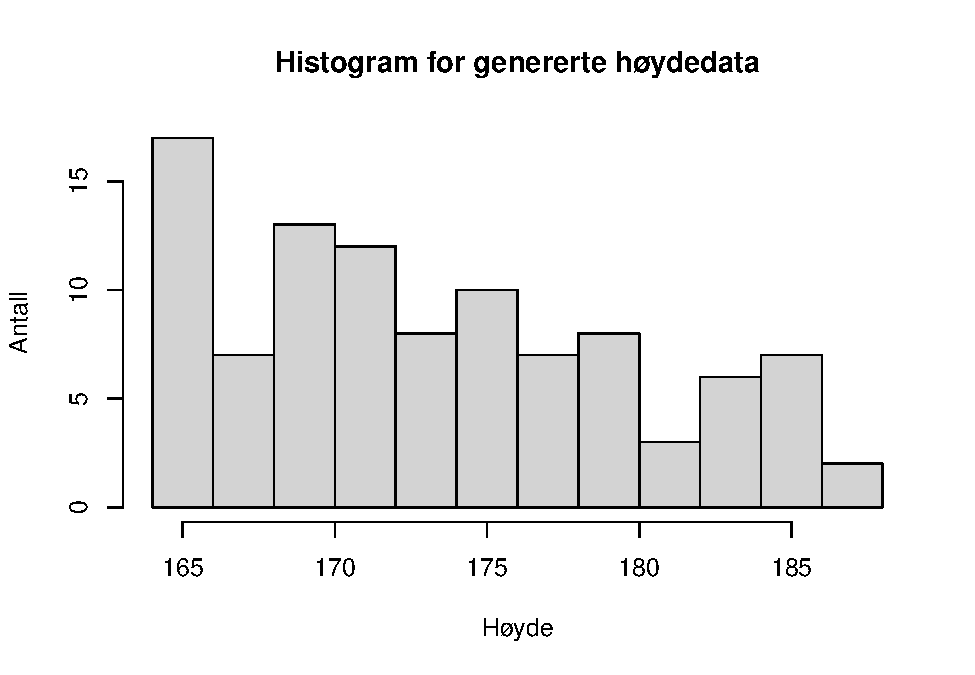
\includegraphics{SPC-book_files/figure-latex/unnamed-chunk-20-1.pdf}
\caption{\label{fig:unnamed-chunk-20}Høydefordeling for 100 andre tilfeldige menn, genererte data}
\end{figure}

Hver gang vi måler høyden på 100 tilfeldig utvalgte menn vil fordelingen se ulik ut siden de er observerte fordelinger i et utvalg av populasjonen (alle) «norske menn». Hvis vi imidlertid økte antallet i utvalget vi målte til 1000 eller 10000 vil vi med større sikkerhet kunne si at vi faktisk viser populasjonens fordeling (mulighetene for at vi tilfeldigvis måler 10000 veldig lave eller veldig høye menn er svært liten). Vi kan derfor, gitt visse forutsetninger om utvalget, si noe om hele populasjonen ut fra utvalget.

Hittil har vi snakket om observerte fordelinger. Ut fra dette kan vi si at vi kan ha visse forventninger til hvordan fordelingen av ulike populasjoner vil se ut, og vi kan snakke om teoretiske fordelinger -- eller sannsynlighetsfordelinger med andre ord. Hvor sannsynlig er det at en tilfeldig x-verdi dukker opp i dataene? For høyde kan vi ha visse forventninger til hvilke sannsynligheter det er for at en tilfeldig person har en gitt høyde, eller hvor mange prosent av den mannlige befolkningen som har en høyde innenfor et gitt intervall. Det vil si at fordelingen har en viss form med visse karakteristika. Vi forventer at flest observasjoner befinner seg i nærheten av gjennomsnittet, og at vi vil se færre og færre observasjoner jo lenger unna gjennomsnittet vi beveger oss. Vi forventer å finne flere norske menn over 20 år på rundt 180 cm enn 160 cm eller 210 cm. For fordelingen av høydedata vil vi si at dette er data som er normalfordelte.

En normalfordeling er en sannsynlighetsfunksjon der flesteparten av verdiene fra funksjonen samler seg om en sentral tendens, og der tettheten (hyppigheten) av verdier avtar jevnt jo lenger unna den sentrale tendensen man kommer. Grafisk framstilt får fordelingskurven en klokkeform, og normalfordeling omtales også som ``bell shaped.'' Overraskende mange fenomener viser seg å være nærme en normalfordeling, og den er derfor en helt sentral teoretisk sannsynlighetsfordeling i mange sammenhenger (også i statistisk prosesskontroll som vi kommer tilbake til senere). Vi bruker dermed normalfordelingen som en modell for observerte data. I en såkalt standard normalfordeling har vi en symmetrisk fordeling der den sentrale tendensen (forventingen) verdi = 0 og et standardavvik = 1.

Vi skal her ikke bry oss om det matematisk uttrykket for sannsynlighetstetthetsfunksjonen. Hvis vi derimot genererer et tenkt datasett etter standard normalfordelingsfunksjon vil det kunne se slik ut:

\begin{figure}
\centering
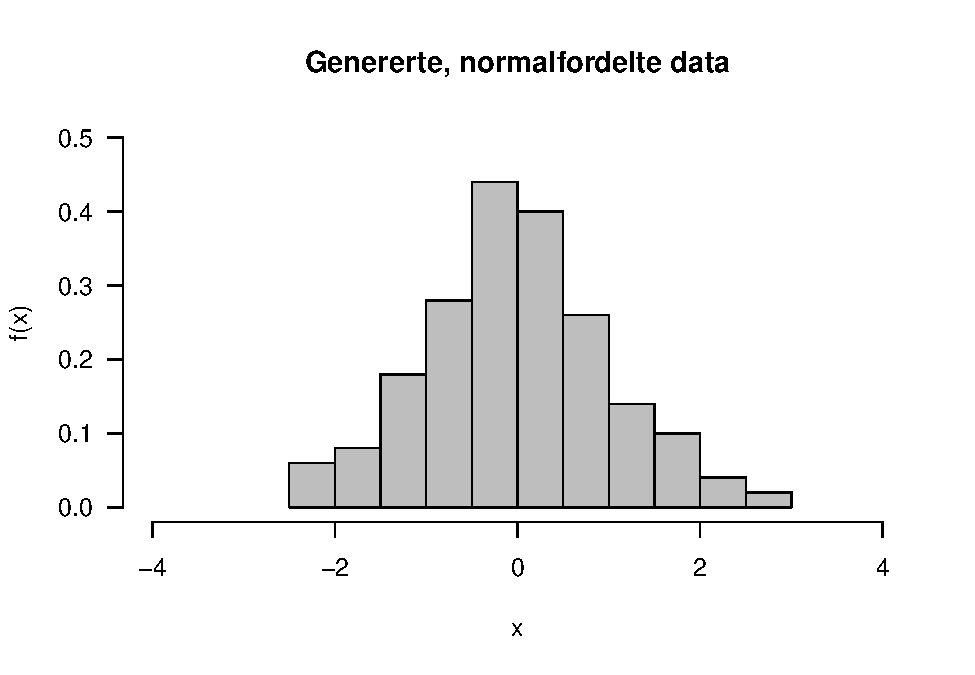
\includegraphics{SPC-book_files/figure-latex/unnamed-chunk-21-1.pdf}
\caption{\label{fig:unnamed-chunk-21}Genererte standard normalfordelte data}
\end{figure}

Her kan vi legge på en forventningskurve -- en teoretisk kurve som viser en standard normalfordeling:

\begin{figure}
\centering
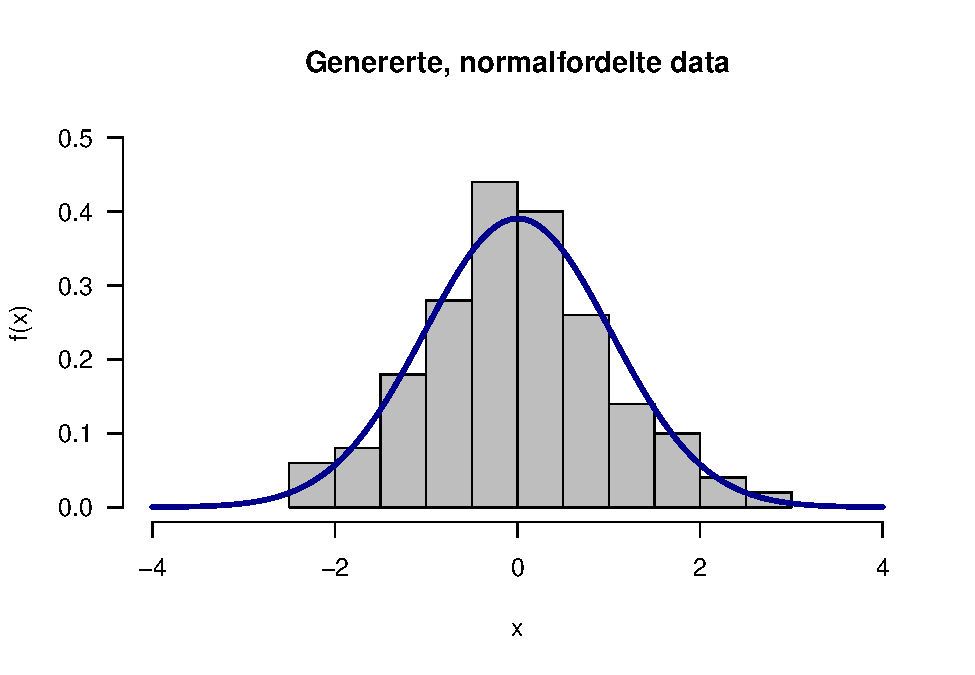
\includegraphics{SPC-book_files/figure-latex/unnamed-chunk-22-1.pdf}
\caption{\label{fig:unnamed-chunk-22}Genererte standard normalfordelte data med normalfordelingskurve}
\end{figure}

Vi kan ta bort det genererte datasettet og sitte igjen med bare normalfordelingskurven:

\begin{figure}
\centering
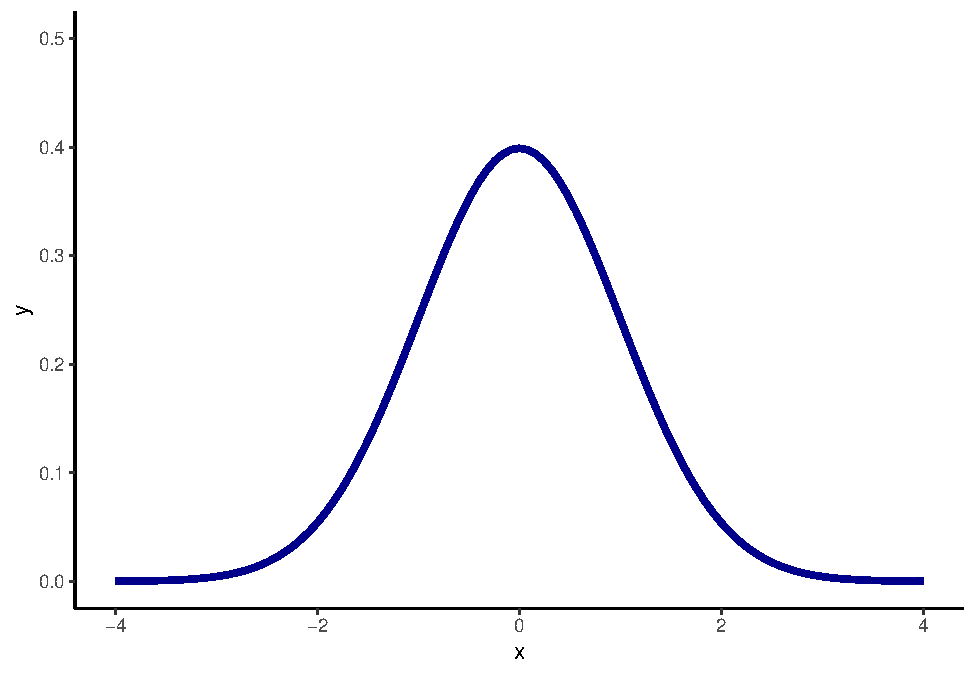
\includegraphics{SPC-book_files/figure-latex/unnamed-chunk-23-1.pdf}
\caption{\label{fig:unnamed-chunk-23}Normalfordelingskurve}
\end{figure}

Det den standardiserte normalfordelingskurven (også kjent som Gausskurven eller også Bellkurven -- ``Klokkekurven'' fordi den har en klokkeform) -- kan brukes til er å si noe om spredningen på forventede verdier -- eller hvor langt fra gjennomsnittsverdien man kan forvente å finne de enkelte verdiene.

Før vi ser nærmere på egenskaper ved normalfordelingskurven kan det være nødvendig å gå litt inn på begrepene varians og standardavvik som mål på spredningen i datasett. Disse begrepene, spesielt standardavvik, vil være helt sentrale i videre arbeid med temaet.

\hypertarget{varians-og-standardavvik}{%
\subsection{Varians og standardavvik}\label{varians-og-standardavvik}}

Variansen i en variabel representerer det gjennomsnittlige avviket fra gjennomsnittsverdien (Field, Miles, and Field 2012) og er et mål på spredningen i dataene (som navnet antyder: hvor mye dataene variere ut fra den sentrale tendensen). Under vises et eksempel basert på Field (2009).

La oss anta at vi har spurt 5 studenter på høgskolen hvor mange kjæledyr de har. Svarene kan settes opp i en enkel tabell. I gjennomsnitt har de 2,6 kjæledyr. Vi ønsker imidlertid å se hvor mye avviket er for den enkelte fra snittet (siden vi har regnet ut snittet kan vi se på gjennomsnittsverdien som en modell på forholdet mellom studenter og antall kjæledyr). Vi registrerer svarene vi fikk i et skjema:

\providecommand{\docline}[3]{\noalign{\global\setlength{\arrayrulewidth}{#1}}\arrayrulecolor[HTML]{#2}\cline{#3}}

\setlength{\tabcolsep}{2pt}

\renewcommand*{\arraystretch}{1.5}

\begin{longtable}[c]{cccc}



\hhline{>{\arrayrulecolor[HTML]{666666}\global\arrayrulewidth=2pt}->{\arrayrulecolor[HTML]{666666}\global\arrayrulewidth=2pt}->{\arrayrulecolor[HTML]{666666}\global\arrayrulewidth=2pt}->{\arrayrulecolor[HTML]{666666}\global\arrayrulewidth=2pt}-}

\multicolumn{1}{!{\color[HTML]{000000}\vrule width 0pt}>{}l}{\fontsize{11}{11}\selectfont{\textcolor[HTML]{000000}{Studentnr}}} & \multicolumn{1}{!{\color[HTML]{000000}\vrule width 0pt}>{}l}{\fontsize{11}{11}\selectfont{\textcolor[HTML]{000000}{Antall}}} & \multicolumn{1}{!{\color[HTML]{000000}\vrule width 0pt}>{}l}{\fontsize{11}{11}\selectfont{\textcolor[HTML]{000000}{Avvik}}} & \multicolumn{1}{!{\color[HTML]{000000}\vrule width 0pt}>{}l!{\color[HTML]{000000}\vrule width 0pt}}{\fontsize{11}{11}\selectfont{\textcolor[HTML]{000000}{Avvik\_kvadrert}}} \\

\hhline{>{\arrayrulecolor[HTML]{666666}\global\arrayrulewidth=2pt}->{\arrayrulecolor[HTML]{666666}\global\arrayrulewidth=2pt}->{\arrayrulecolor[HTML]{666666}\global\arrayrulewidth=2pt}->{\arrayrulecolor[HTML]{666666}\global\arrayrulewidth=2pt}-}

\endfirsthead

\hhline{>{\arrayrulecolor[HTML]{666666}\global\arrayrulewidth=2pt}->{\arrayrulecolor[HTML]{666666}\global\arrayrulewidth=2pt}->{\arrayrulecolor[HTML]{666666}\global\arrayrulewidth=2pt}->{\arrayrulecolor[HTML]{666666}\global\arrayrulewidth=2pt}-}

\multicolumn{1}{!{\color[HTML]{000000}\vrule width 0pt}>{}l}{\fontsize{11}{11}\selectfont{\textcolor[HTML]{000000}{Studentnr}}} & \multicolumn{1}{!{\color[HTML]{000000}\vrule width 0pt}>{}l}{\fontsize{11}{11}\selectfont{\textcolor[HTML]{000000}{Antall}}} & \multicolumn{1}{!{\color[HTML]{000000}\vrule width 0pt}>{}l}{\fontsize{11}{11}\selectfont{\textcolor[HTML]{000000}{Avvik}}} & \multicolumn{1}{!{\color[HTML]{000000}\vrule width 0pt}>{}l!{\color[HTML]{000000}\vrule width 0pt}}{\fontsize{11}{11}\selectfont{\textcolor[HTML]{000000}{Avvik\_kvadrert}}} \\

\hhline{>{\arrayrulecolor[HTML]{666666}\global\arrayrulewidth=2pt}->{\arrayrulecolor[HTML]{666666}\global\arrayrulewidth=2pt}->{\arrayrulecolor[HTML]{666666}\global\arrayrulewidth=2pt}->{\arrayrulecolor[HTML]{666666}\global\arrayrulewidth=2pt}-}\endhead



\multicolumn{1}{!{\color[HTML]{000000}\vrule width 0pt}>{}l}{\fontsize{11}{11}\selectfont{\textcolor[HTML]{000000}{1}}} & \multicolumn{1}{!{\color[HTML]{000000}\vrule width 0pt}>{}l}{\fontsize{11}{11}\selectfont{\textcolor[HTML]{000000}{1}}} & \multicolumn{1}{!{\color[HTML]{000000}\vrule width 0pt}>{}l}{\fontsize{11}{11}\selectfont{\textcolor[HTML]{000000}{-1.6}}} & \multicolumn{1}{!{\color[HTML]{000000}\vrule width 0pt}>{}l!{\color[HTML]{000000}\vrule width 0pt}}{\fontsize{11}{11}\selectfont{\textcolor[HTML]{000000}{2.56}}} \\





\multicolumn{1}{!{\color[HTML]{000000}\vrule width 0pt}>{}l}{\fontsize{11}{11}\selectfont{\textcolor[HTML]{000000}{2}}} & \multicolumn{1}{!{\color[HTML]{000000}\vrule width 0pt}>{}l}{\fontsize{11}{11}\selectfont{\textcolor[HTML]{000000}{2}}} & \multicolumn{1}{!{\color[HTML]{000000}\vrule width 0pt}>{}l}{\fontsize{11}{11}\selectfont{\textcolor[HTML]{000000}{-0.6}}} & \multicolumn{1}{!{\color[HTML]{000000}\vrule width 0pt}>{}l!{\color[HTML]{000000}\vrule width 0pt}}{\fontsize{11}{11}\selectfont{\textcolor[HTML]{000000}{0.36}}} \\





\multicolumn{1}{!{\color[HTML]{000000}\vrule width 0pt}>{}l}{\fontsize{11}{11}\selectfont{\textcolor[HTML]{000000}{3}}} & \multicolumn{1}{!{\color[HTML]{000000}\vrule width 0pt}>{}l}{\fontsize{11}{11}\selectfont{\textcolor[HTML]{000000}{3}}} & \multicolumn{1}{!{\color[HTML]{000000}\vrule width 0pt}>{}l}{\fontsize{11}{11}\selectfont{\textcolor[HTML]{000000}{0.4}}} & \multicolumn{1}{!{\color[HTML]{000000}\vrule width 0pt}>{}l!{\color[HTML]{000000}\vrule width 0pt}}{\fontsize{11}{11}\selectfont{\textcolor[HTML]{000000}{0.16}}} \\





\multicolumn{1}{!{\color[HTML]{000000}\vrule width 0pt}>{}l}{\fontsize{11}{11}\selectfont{\textcolor[HTML]{000000}{4}}} & \multicolumn{1}{!{\color[HTML]{000000}\vrule width 0pt}>{}l}{\fontsize{11}{11}\selectfont{\textcolor[HTML]{000000}{3}}} & \multicolumn{1}{!{\color[HTML]{000000}\vrule width 0pt}>{}l}{\fontsize{11}{11}\selectfont{\textcolor[HTML]{000000}{0.4}}} & \multicolumn{1}{!{\color[HTML]{000000}\vrule width 0pt}>{}l!{\color[HTML]{000000}\vrule width 0pt}}{\fontsize{11}{11}\selectfont{\textcolor[HTML]{000000}{0.16}}} \\





\multicolumn{1}{!{\color[HTML]{000000}\vrule width 0pt}>{}l}{\fontsize{11}{11}\selectfont{\textcolor[HTML]{000000}{5}}} & \multicolumn{1}{!{\color[HTML]{000000}\vrule width 0pt}>{}l}{\fontsize{11}{11}\selectfont{\textcolor[HTML]{000000}{4}}} & \multicolumn{1}{!{\color[HTML]{000000}\vrule width 0pt}>{}l}{\fontsize{11}{11}\selectfont{\textcolor[HTML]{000000}{1.4}}} & \multicolumn{1}{!{\color[HTML]{000000}\vrule width 0pt}>{}l!{\color[HTML]{000000}\vrule width 0pt}}{\fontsize{11}{11}\selectfont{\textcolor[HTML]{000000}{1.96}}} \\





\multicolumn{1}{!{\color[HTML]{000000}\vrule width 0pt}>{}l}{\fontsize{11}{11}\selectfont{\textcolor[HTML]{000000}{Snitt}}} & \multicolumn{1}{!{\color[HTML]{000000}\vrule width 0pt}>{}l}{\fontsize{11}{11}\selectfont{\textcolor[HTML]{000000}{2.6}}} & \multicolumn{1}{!{\color[HTML]{000000}\vrule width 0pt}>{}l}{\fontsize{11}{11}\selectfont{\textcolor[HTML]{000000}{}}} & \multicolumn{1}{!{\color[HTML]{000000}\vrule width 0pt}>{}l!{\color[HTML]{000000}\vrule width 0pt}}{\fontsize{11}{11}\selectfont{\textcolor[HTML]{000000}{}}} \\





\multicolumn{1}{!{\color[HTML]{000000}\vrule width 0pt}>{}l}{\fontsize{11}{11}\selectfont{\textcolor[HTML]{000000}{Sum}}} & \multicolumn{1}{!{\color[HTML]{000000}\vrule width 0pt}>{}l}{\fontsize{11}{11}\selectfont{\textcolor[HTML]{000000}{}}} & \multicolumn{1}{!{\color[HTML]{000000}\vrule width 0pt}>{}l}{\fontsize{11}{11}\selectfont{\textcolor[HTML]{000000}{0}}} & \multicolumn{1}{!{\color[HTML]{000000}\vrule width 0pt}>{}l!{\color[HTML]{000000}\vrule width 0pt}}{\fontsize{11}{11}\selectfont{\textcolor[HTML]{000000}{5.20}}} \\

\hhline{>{\arrayrulecolor[HTML]{666666}\global\arrayrulewidth=2pt}->{\arrayrulecolor[HTML]{666666}\global\arrayrulewidth=2pt}->{\arrayrulecolor[HTML]{666666}\global\arrayrulewidth=2pt}->{\arrayrulecolor[HTML]{666666}\global\arrayrulewidth=2pt}-}



\end{longtable}

Når vi regner ut avviket (sum of deviances) summerer vi avvikene. Siden denne er 0 skulle det innebære at det totalt sett i ``modellen'' ikke er avvik mellom modellen og våre virkelige observasjoner. Problemet her er at det er både positive og negative avvik som nuller hverandre ut. Man må derfor kvadrere avvikene for å omgå problemet med fortegn. Imidlertid får vi et nytt problem. La oss anta at vi i stedet for 5 studenter har spurt 500. Da får vi et svært høyt kvadrert avvik fra snitt. Altså -- vi må ta høyde for for antallet observasjoner. Vi deler derfor sum kvadrert avvik fra snitt på antall observasjoner (5,20/5). MEN: vi må foreta et litt teknisk og komplisert tillegg i utregningen. Vi må dele på antall observasjoner MINUS 1 (som er antallet frihetsgrader -- degrees of freedom). Dette vil ikke bli nærmere forklart her, men for de som ønsker å lese mer om frihetsgrader kan prøve noen andre kilder, f.eks. Walker (1940), Good (1973) eller Pandey and Bright (2008). Vi ender altså opp med regnestykket 5,20/(5-1) = 1,3. Dette er variansen. \emph{Variansen er altså det gjennomsnittlige avviket mellom gjennomsnittsverdien av de observerte dataene og verdiene til de enkelte observasjonene.}

Som regel snakker vi imidlertid om standardavviket. Dette finner vi ved å ta kvadratroten av variansen (som vi jo har funnet ved å kvadrere avvikene for å unngå fortegnsproblemer). Vi får da i vårt tilfelle et standardavvik på 1,14. Variansen og standardavviket forteller oss altså noe om spredningen i dataene. Liten varians betyr at spredningen er liten (om vi har gjennomført en spørreundersøkelse betyr det at respondentene har svart ganske likt). Stor varians betyr stor spredning (respondentene har svart ganske ulikt).

\hypertarget{normalfordeling-standardavvik-og-forventninger}{%
\subsection{Normalfordeling, standardavvik og forventninger}\label{normalfordeling-standardavvik-og-forventninger}}

Vi kan nå se nærmere på normalfordelingen.

\begin{figure}
\centering
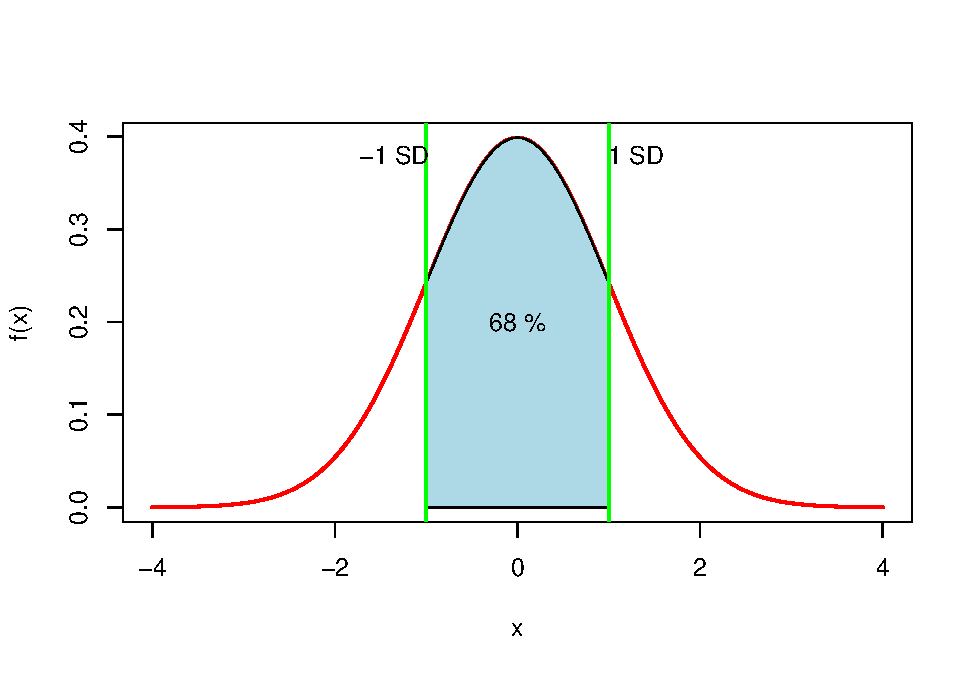
\includegraphics{SPC-book_files/figure-latex/unnamed-chunk-25-1.pdf}
\caption{\label{fig:unnamed-chunk-25}Normalfordeling med 1 standardavvik}
\end{figure}

Ett standardavvik ``over og under'' 0 (= det skraverte området i grafen over) innebærer at det er 68 \% sannsynlighet for at en tilfeldig valgt x-verdi befinner seg i dette intervallet. Vi kan vise det samme for 2 og 3 standardavvik:

\begin{figure}
\centering
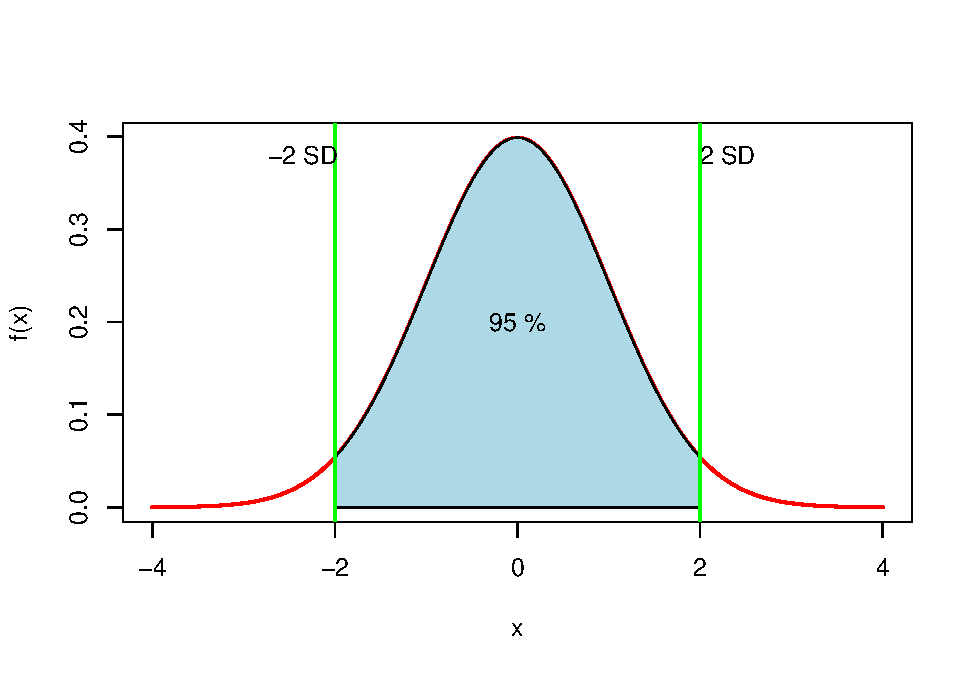
\includegraphics{SPC-book_files/figure-latex/unnamed-chunk-26-1.pdf}
\caption{\label{fig:unnamed-chunk-26}Normalfordeling med 2 standardavvik}
\end{figure}

To standardavvik ``over og under'' 0 (= det skraverte området i grafen over) innebærer at det er 95 \% sannsynlighet for at en tilfeldig valgt x-verdi befinner seg i dette intervallet. Vi kan finne arealet mellom x=-2 og x=2, som er 0.9544997\footnote{R-kode for utregning av areal mellom to x-verdier i en normalfordeing (=sannsynlighet for at en gitt x-verdi ligger i intervallet mellom de to x-verdiene): pnorm(2,mean=0,sd=1)-pnorm(-2,mean=0,sd=1)}.

\begin{figure}
\centering
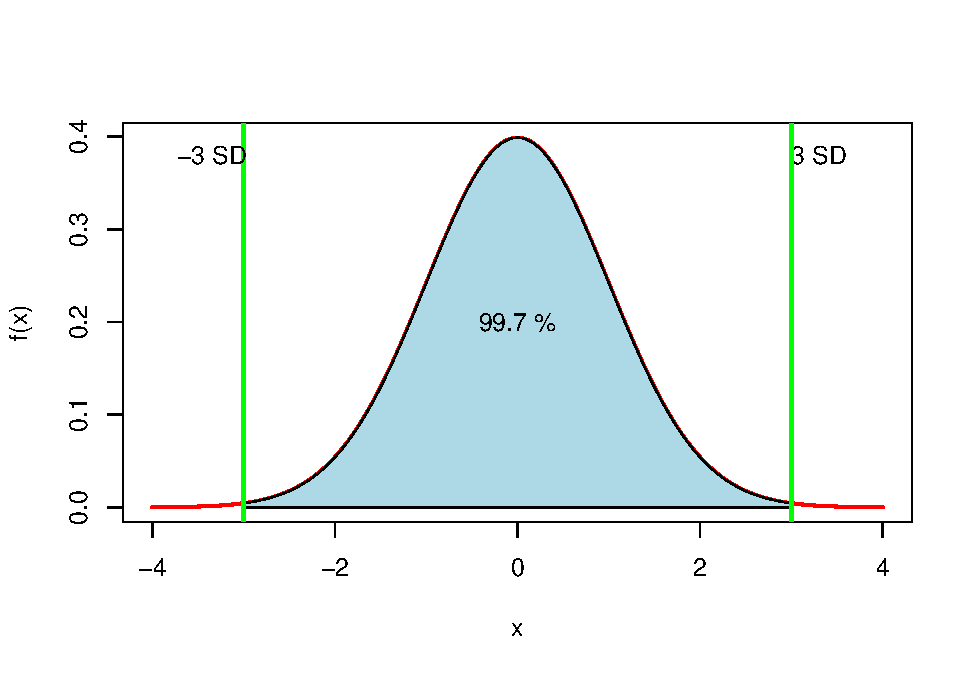
\includegraphics{SPC-book_files/figure-latex/unnamed-chunk-27-1.pdf}
\caption{\label{fig:unnamed-chunk-27}Normalfordeling med 3 standardavvik}
\end{figure}

Tre standardavvik ``over og under'' 0 (= det skraverte området i grafen over) innebærer at det er 99.7 \% sannsynlighet for at en tilfeldig valgt x-verdi befinner seg i dette intervallet. Vi kan finne arealet mellom x=-3 og x=3, som er 0.9973002\footnote{pnorm(3,mean=0,sd=1)-pnorm(-3,mean=0,sd=1)}. Dette utgjør et kjernepunkt i statistisk prosesskontroll som vi vil komme mye tilbake til.

Oppsummert kan vi framstille normalfodeling og standardavvik slik (Hartmann, Krois, and Waske 2018b):

\begin{figure}
\centering
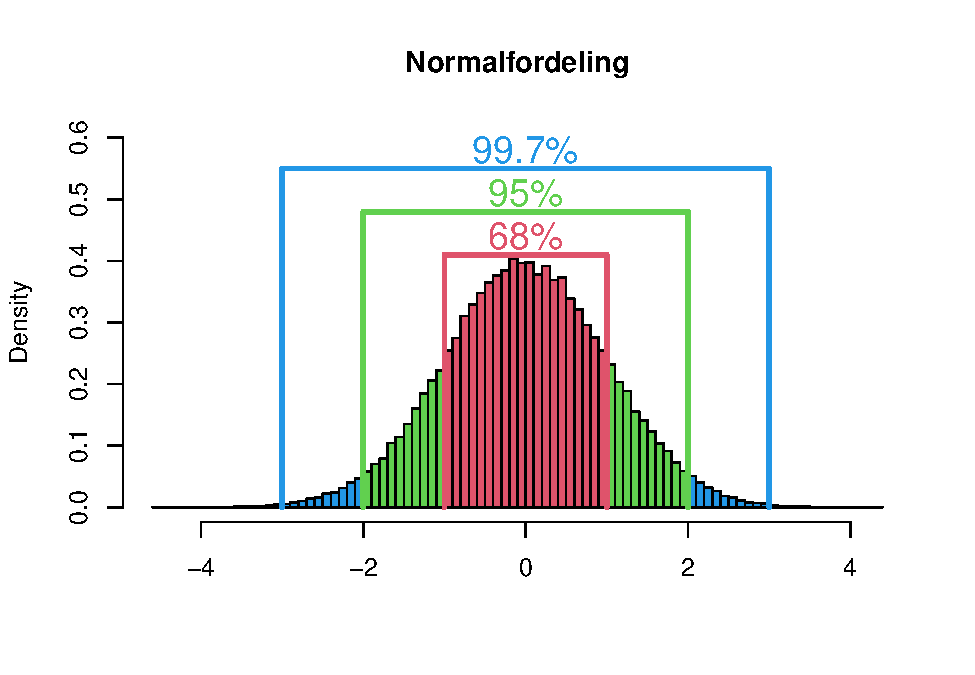
\includegraphics{SPC-book_files/figure-latex/unnamed-chunk-28-1.pdf}
\caption{\label{fig:unnamed-chunk-28}Normalfordeling med standardavvik}
\end{figure}

Som nevnt er mange fenomener i hverdagen normalfordelte, eller nærme nok normalfordeling til at vi kan bruke normalfordeling som teoretisk modell for observerte data.\footnote{Normalfordelingen er dessuten en god tilnærming til binomialfordeling med høyt antall observasjoner (høy n), og også til poissonfordeling med høy frekvens. Dette forfølger vi imidlertid ikke videre i dette kompendiet.} Det finnes imidlertid mange tilfeller der vi ikke kan bruke normalfordelingen. Hvis dataene er sterkt asymmetriske vil ikke reglene for normalfordeling som vi har skissert ovenfor gjelde.\footnote{Chebyshevs teorem vil imidlertid gjelde for alle datasett. Teoremet belyses i eget vedlegg for de spesielt interesserte} Noen av de er viktige for statistisk prosesskontroll, og de vil vi se på i de følgende avsnittene.

\hypertarget{binomialfordeling}{%
\section{Binomialfordeling}\label{binomialfordeling}}

En distribusjon hvor det kun er to mulige utfall av en hendelse kalles en binomial fordeling. Et myntkast er en slik hendelse (gitt at vi ser bort fra den fysiske muligheten at mynten kan lande stående på høykant). Levende eller død kan også være et eksempel på dette. Det ene utfallet utelukker det andre, men de er uavhengige fordi resultatet i ett myntkast ikke påvirker resultatet i neste myntkast. Alle myntkastene må derimot være identiske, det vil si sannsynligheten for det ene eller det andre resultatet er lik hver gang forsøket eller myntkastet gjennomføres. Hvis vi har lik sannsynlighet, kan en tilfeldig generert binomial distribusjon se slik ut:

\begin{figure}
\centering
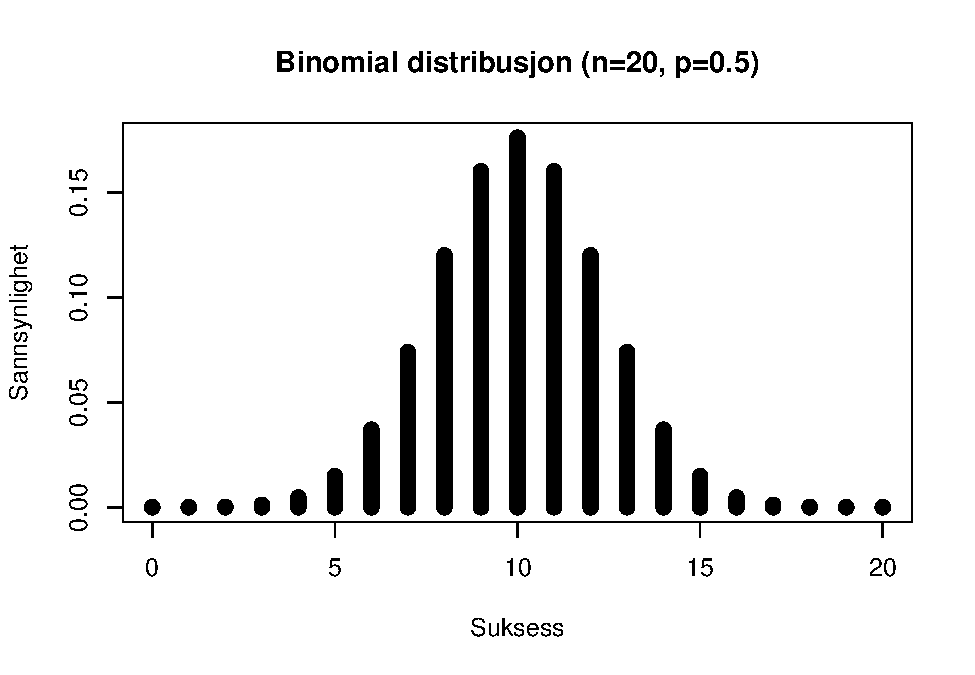
\includegraphics{SPC-book_files/figure-latex/unnamed-chunk-29-1.pdf}
\caption{\label{fig:unnamed-chunk-29}Binomialfordeling med lik sannsynlighet}
\end{figure}

I diagrammet over vises en sannsynlighetsfordeling for en binomial fordeling der utfallene suksess/fiasko har lik sannsynlighet. Hvis vi gjennomfører en aktivitet med disse karakteristika 20 ganger kan vi bruke sannsynlighetsfordelingen til å skape en forventning om sannsynligheten for antall suksesser/fiaskoer. Hver gang vi gjennomfører aktiviteten blir det enten suksess eller fiasko. Hvis vi har 50\% sjanse for suksess eller feil hver gang vi gjennomfører aktiviteten er sannsynligheten for suksess lik som sannsynligheten for fiasko. Vi kan da forvente at det er størst sannsynlighet at vi i 10 av 20 tilfeller får suksess. Det er liten sannsynlighet for at vi enten får suksess i 0 eller 20 av 20 ganger vi gjør aktiviteten.

Det er imidlertid verdt å merke seg at de to utfallene ikke trenger å ha lik sannsynlighet. Da vil den binomiale distribusjonen se annerledes ut:

\begin{figure}
\centering
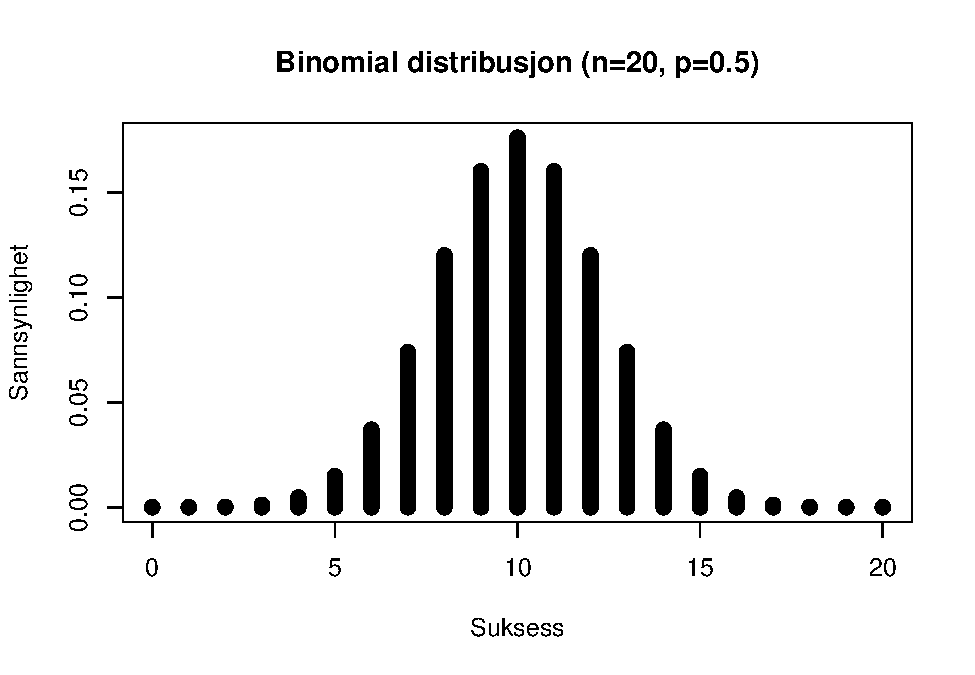
\includegraphics{SPC-book_files/figure-latex/unnamed-chunk-30-1.pdf}
\caption{\label{fig:unnamed-chunk-30}Binomialfordeling med ulik sannsynlighet}
\end{figure}

Her har vi bare 20\% sannsynlighet for suksess, og fordelingen av sannsynligheter vil se annerledes ut. Med 20\% sannsynlighet for suksess er det veldig liten sannsynlighet for at vi vil få 10 eller flere suksesser hvis vi gjør forsøket 20 ganger. Det er størst sannsynlighet for å få 4 suksesser.

Et terningkast (med en vanlig terning med 6 sider) -- som ikke er tuklet med -- har lik sannsynlighet for å lande på hhv 1,2,3,4,5 og 6. Det vil si det er 1/6 sannsynlighet for 1, 1/6 sannsynlighet for 2 osv. Hvis vi kaster denne terningen 10 ganger kan resultatet se slik ut:

\begin{figure}
\centering
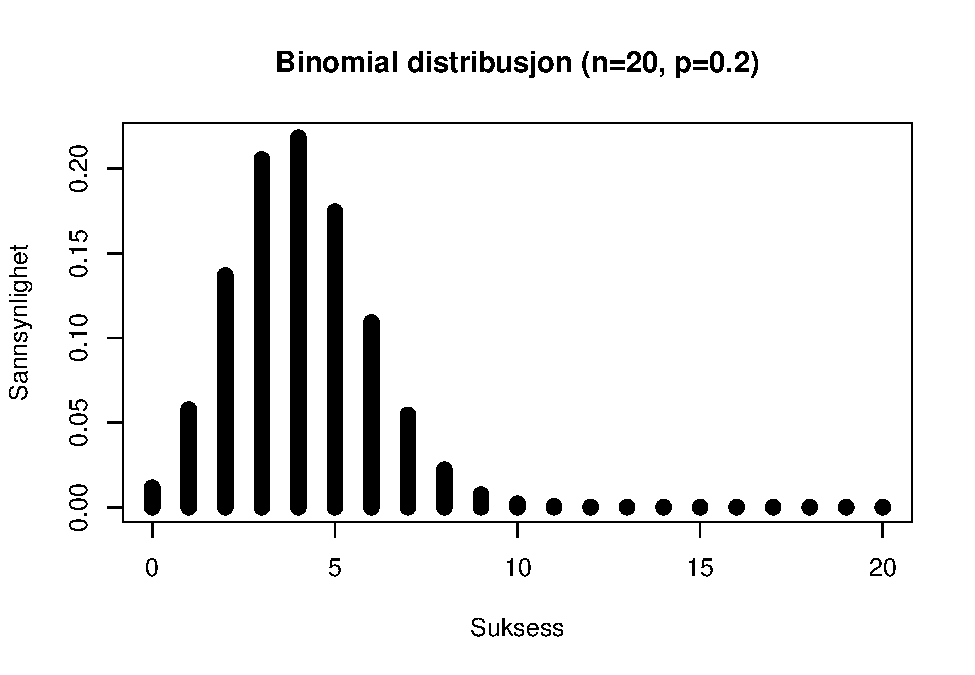
\includegraphics{SPC-book_files/figure-latex/unnamed-chunk-31-1.pdf}
\caption{\label{fig:unnamed-chunk-31}10 terningkast}
\end{figure}

Vi ser at vi ikke fikk noen 2'ere og 5'ere. Dette kan vi forvente når vi bare har 10 terningkast. Hvis vi imidlertid kaster terningen 100 ganger vil det være svært liten sannsynlighet for å ikke få «treff» på alle 6 verdiene på terningen, og vi burde kunne forvente at vi får en ganske jevn fordeling på alle 6 verdiene. Nedenfor vises resultatet av 100 terningkast.

\begin{figure}
\centering
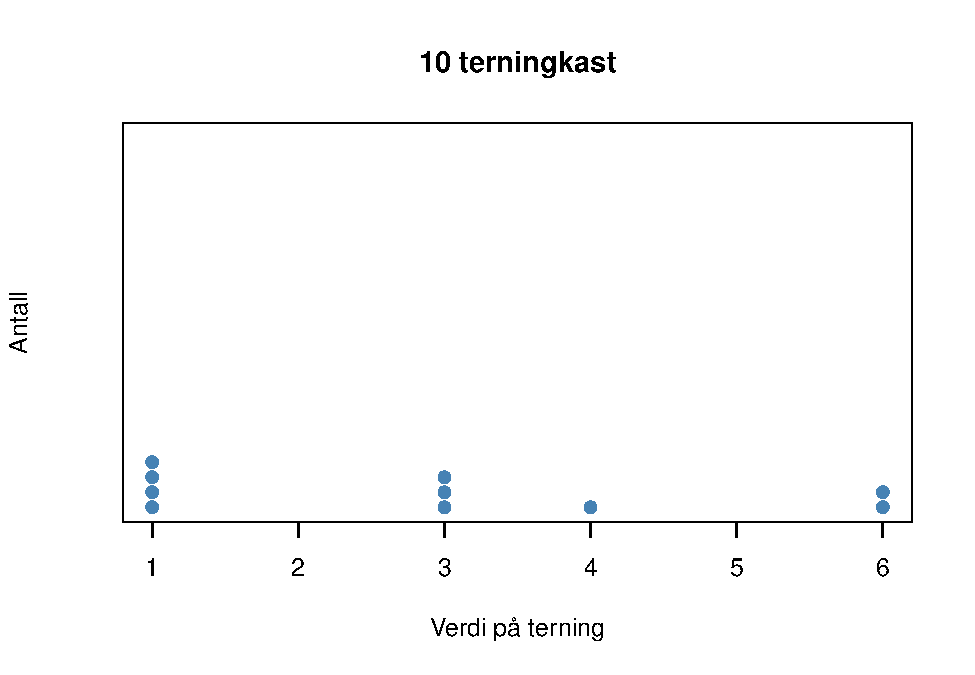
\includegraphics{SPC-book_files/figure-latex/unnamed-chunk-32-1.pdf}
\caption{\label{fig:unnamed-chunk-32}100 terningkast}
\end{figure}

Vi ser at vi har en relativt jevn fordeling. Noe ulikhet er det selvsagt, noe vi vil forvente fra en tilfeldig prosess. Hvis vi gjennomførte 1000 eller 10000 terningkast vil fordelingen bli nærmere og nærmere den teoretisk forventede fordelingen. Vi kan burde, teoretisk, forvente 100 treff på hver mulighet hvis vi kaster terningen 600 ganger, men vi vil sjelden se akkurat 100 treff på hver slik vi ser hvis vi kjører tre runder med 600 terningkast:

Runde 1:

\begin{verbatim}
## terning_runde1
##   1   2   3   4   5   6 
##  93 102 102 102 108  93
\end{verbatim}

Runde 2:

\begin{verbatim}
## terning_runde2
##   1   2   3   4   5   6 
## 101 102  94  91 105 107
\end{verbatim}

Runde 3:

\begin{verbatim}
## terning_runde3
##   1   2   3   4   5   6 
## 104 113  92  98  95  98
\end{verbatim}

Selv om vi kjører 6 000 000 terningkast og vil forvente 1 000 000 treff på hver av terningens sider vil vi ikke få en perfekt fordeling iht teoretisk forventning, men resultatet vil være svært nærme og er nærme nok til at vi kan bruke sannsynlighetsfordelingen til å lage forventninger om utfall:

6 000 000 terningkast:

\begin{verbatim}
## minterning
##       1       2       3       4       5       6 
## 1000492  998250 1000216 1000832 1001422  998788
\end{verbatim}

Hvis vi setter resultatet fra 6 000 000 terningkast inn i et histogram ser vi at resultatet er svært nærme hva vi teoretisk vil forvente:

\begin{figure}
\centering
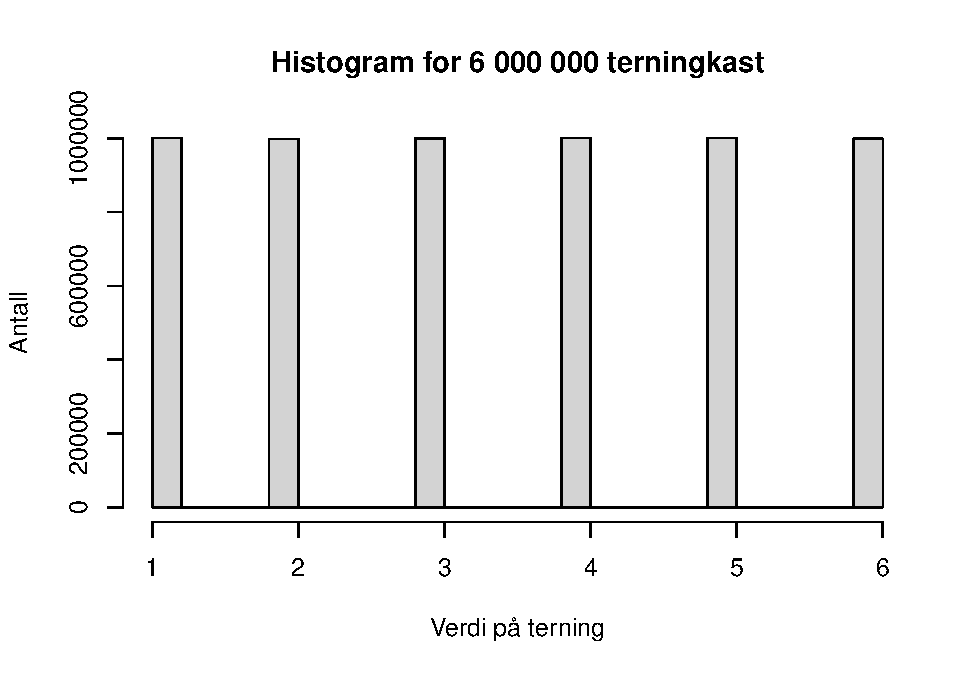
\includegraphics{SPC-book_files/figure-latex/unnamed-chunk-37-1.pdf}
\caption{\label{fig:unnamed-chunk-37}6 000 000 terningkast}
\end{figure}

\hypertarget{poissonfordeling}{%
\section{Poissonfordeling}\label{poissonfordeling}}

Poissonfordelinger finnes i situasjoner der hendelser skjer vilkårlig i tid (og rom) hvor vi er interessert i kun antallet hendelser i et gitt tidsintervall. Vi kan f.eks. være interessert i hvor mange supporthenvendelser vi får i løpet av en time, antallet feilmedisineringer per uke, hvor mange besøk avdelingen får per dag o.l. Andre eksempler kan være antall trafikkulykker langs en angitt veistrekning, antall elgpåkjørlser på en togstrekning, eller antall av en gitt art fugler i et definert område i et definert tidsrom. En hendelse må være uavhengig tidsmessig av andre hendelser (det er altså ikke økt sannsynlighet for at en hendelse vil skje fordi en tilsvarende hendelse akkurat har skjedd), sannsynligheten for en hendelse i et kort perspektiv er lik sannsynligheten over et lengre perspektiv, og ettersom et tidsintervall blir kortere og kortere vil sannsynligheten for hendelsen gå mot null.

Poissonfordeling uttrykker sannsynligheten for at et gitt antall hendelser inntreffer i et gitt tidsintervall (eller et gitt geografisk domene) \emph{og} at vi kjenner gjennomsnittlig hvor ofte hendelsen inntreffer. Denne sannsynligheten uttrykkes som en lambdaverdi (\(\lambda\)).

Eksempelet under er hentet fra Soage (2020):

\begin{figure}
\centering
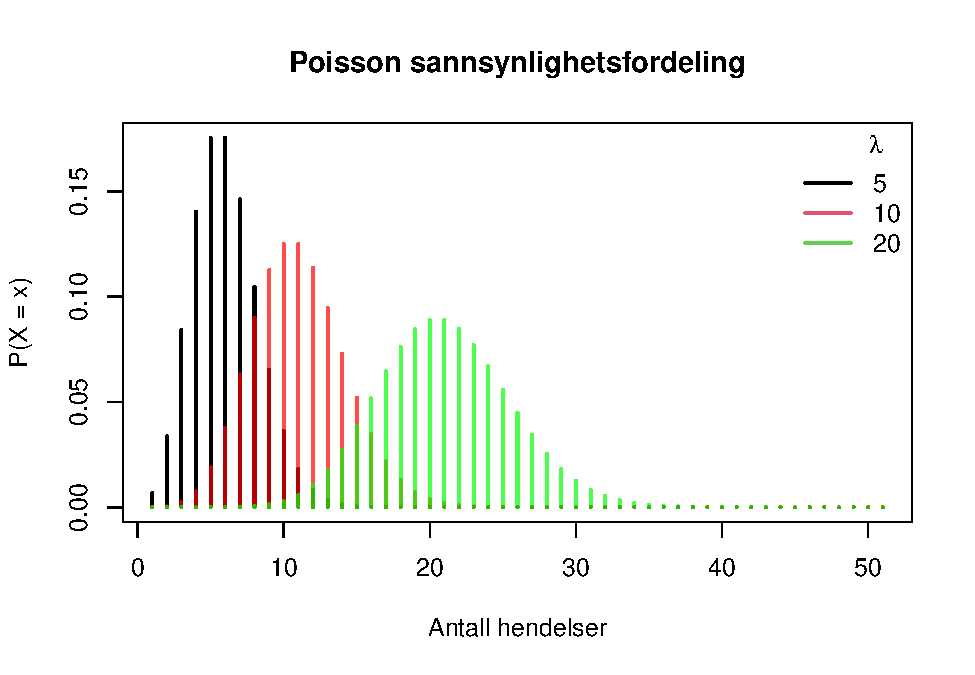
\includegraphics{SPC-book_files/figure-latex/unnamed-chunk-38-1.pdf}
\caption{\label{fig:unnamed-chunk-38}Poissonfordelinger}
\end{figure}

Ut fra hvilken \(\lambda\)-verdi vi setter kan vi si noe om sannsynligheten for at et antall hendelser inntreffer.

Ugarte, Militino, and Arnholt (2016) eksemplifiserer Poissonfordeling ved å vise til at det i gjennomsnitt skåres 2,5 mål i en VM-kamp i fotball. Denne situasjonen tilfredsstiller forutsetningene for å bruke Possionfordeling.Vi kan grafisk framstille sannsynlighetsfordeingen slik:

\begin{figure}
\centering
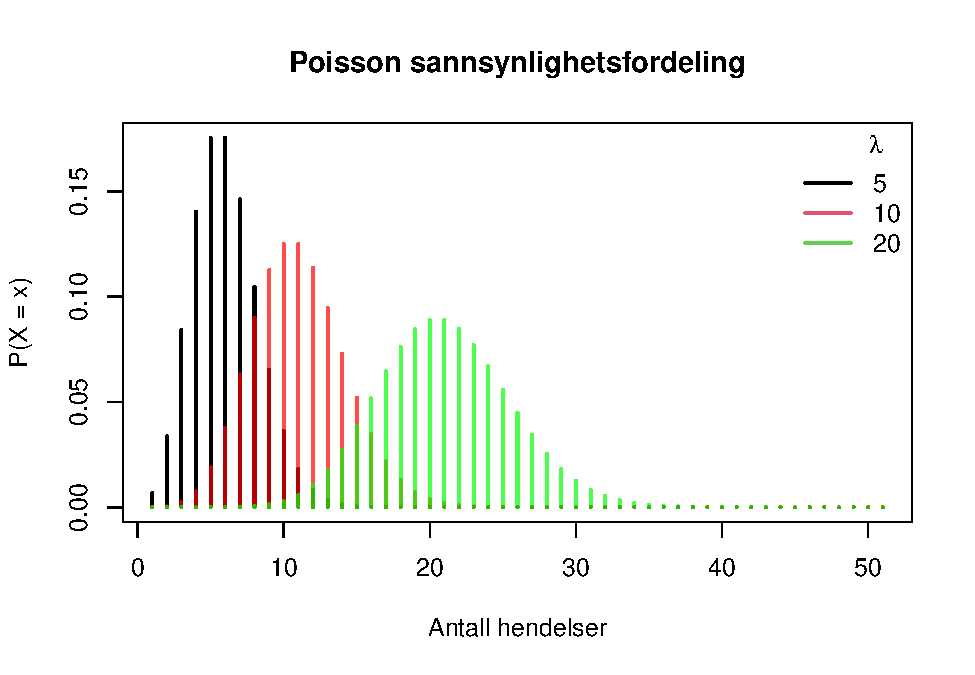
\includegraphics{SPC-book_files/figure-latex/unnamed-chunk-39-1.pdf}
\caption{\label{fig:unnamed-chunk-39}Poissonfordeling mål i VM-kamp fotball}
\end{figure}

I R kan vi også enkelt regne ut den nøyaktige sannsynligheten for x antall mål gitt forutsetningen om at det i snitt skåres 2.5 mål pr kamp til å være 0. Vi kan bruke sannsynlighetsfordelingen til å regne ut sannsynligheten for et gitt antall mål, f.eks.:

\begin{itemize}
\tightlist
\item
  Sannsynligheten for 0 mål = 0.082085
\item
  Sannsynligheten for 1 mål = 0.2052125
\item
  Sannsynligheten for 2 mål = 0.2565156
\item
  Sannsynligheten for 3 mål = 0.213763
\item
  Sannsynligheten for 4 mål = 0.1336019
\end{itemize}

eller f.eks. sannsynligheten for at det skåres mellom 1 og 3 mål (= 0.6754911).

\hypertarget{geometrisk-fordeling}{%
\section{Geometrisk fordeling}\label{geometrisk-fordeling}}

En geometrisk fordeling er en diskret fordeling der man teller antall hendelser/forsøk inntil et gitt resultat forekommer. Resultatet er suksess eller feil, altså hvor mange ganger man har en hendelse før man får en suksess eller feil (avhengig av hva man måler). Et eksempel er hvor mange ganger man må kaste to terninger for å få 11 i sum. Man kaster da to terninger til første gang man får 11 (= suksess). En geometrisk distribusjon kan se slik ut (p = 0,4):

\begin{figure}
\centering
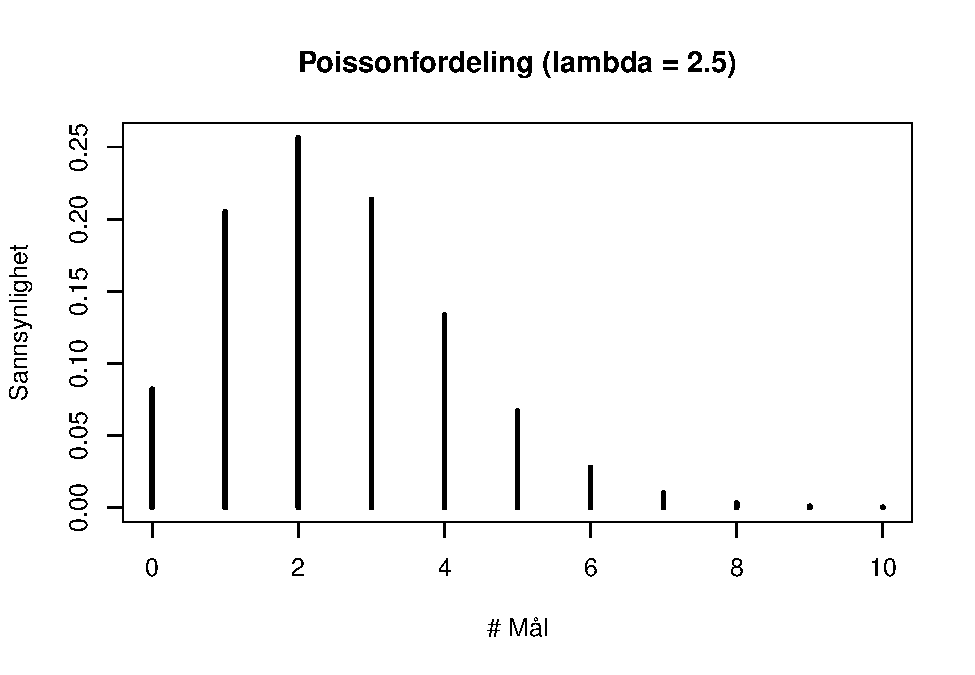
\includegraphics{SPC-book_files/figure-latex/unnamed-chunk-40-1.pdf}
\caption{\label{fig:unnamed-chunk-40}Geometrisk fordeling}
\end{figure}

I statistisk prosesskontroll er denne typen fordeling til stede når man f.eks. teller antall dager mellom sjeldne hendelser. Man teller antall dager før man f.eks. får et alvorlig avvik på en medisinering, en operasjon e.l. I geometrisk fordeling er sannsynligheten for et gitt utfall uavhengig av om det har skjedd før. Man kan bruke geometrisk fordeling f.eks. til å estimere hvor mange dager man normalt vil forvente det går mellom en sjelden hendelse. Hvis man gjennom erfaringstall vet at sannsynligheten for en sjelden hendelse er p = 0.035 vil man forvente at det går 1/0.035 \(\approx\) 29 dager mellom hver hendelse. Geometrisk distribusjon kan hjelpe oss i en statistisk prosesskontroll for å finne normal/unormal variasjon ved sjeldne hendelser.

Det kan være verdt å merke seg at binomial og geometrisk fordeling skiller seg fra hverandre ved at geometrisk fordeling har et ukjent antall hendelser (man fortsetter til man får første suksess/feil), mens binomial fordeling har et gitt antall hendelser. Som vi skal se i senere eksempler derfor geometrisk fordeling viktig når vi håndterer sjeldne hendelser, fordi vi ikke kjenner hvor mange dager det f.eks. går før vi får første suksess/feil.

\hypertarget{eksponensiell-fordeling}{%
\section{Eksponensiell fordeling}\label{eksponensiell-fordeling}}

En tilfeldig kontinuerlig variabel kan sies å være analog til den geometriske distribusjonen, men for kontinuerlige data. Den eksponensielle distribusjonen brukes ofte for å modellere tid mellom to hendelser. I statistisk prosesskontroll vil vi typisk bruke denne distribusjonen hvis vi måler tid mellom to sjeldne hendelser. Hvis vi f.eks. måler tiden mellom uventet dødsfall som følge av en type rutineoperasjon på et sykehus vil den ha en eksponensiell distribusjon hvis sannsynligheten for at hendelsen inntreffer innenfor t gitt tidsintervall er omtrentlig proporsjonal med lengde på tidsintervallet (Taboga 2017). Eksponensielle fordelinger har samme grunnform, men kan ha ulik bratthet avhengig av den såkalte lamdaverdien (= en parameter for raten av hendelser). Lambdaverdi er en parameter for hvor ofte hendelsene forventes å skje.

\begin{figure}
\centering
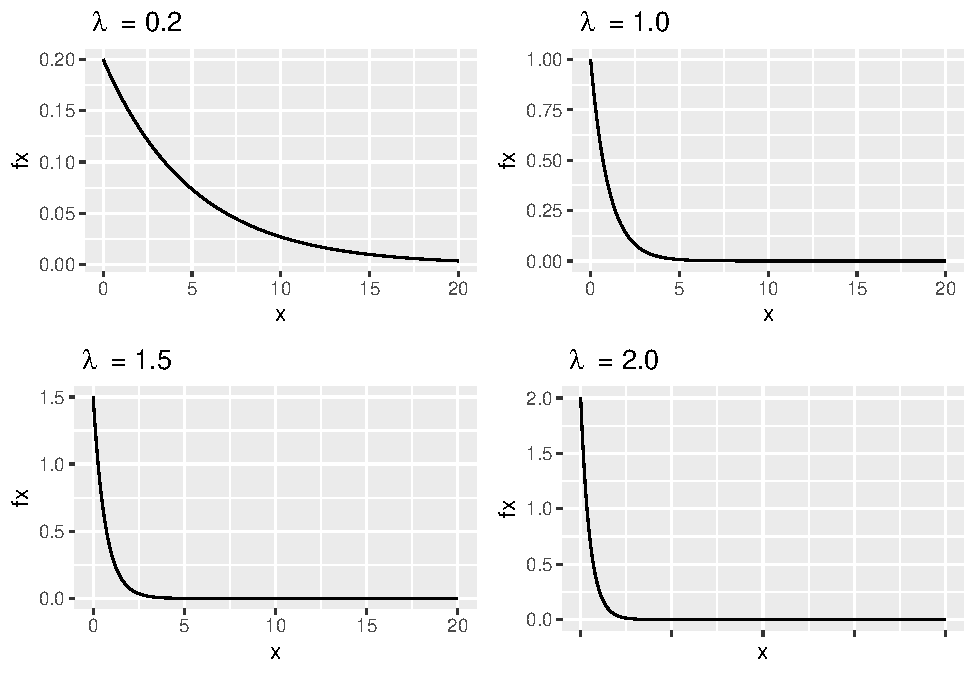
\includegraphics{SPC-book_files/figure-latex/unnamed-chunk-41-1.pdf}
\caption{\label{fig:unnamed-chunk-41}Eksponensiell fordeling}
\end{figure}

\hypertarget{er-dataene-dine-normalfordelte}{%
\chapter{Er dataene dine normalfordelte?}\label{er-dataene-dine-normalfordelte}}

I forrige kapittel viste vi til at data har ulike fordelinger, og at ulike analyser vi gjør i statistisk prosesskontroll har forutsetninger/bygger på antalkelser om hvordan dataene er fordelt (det gjelder forsåvidt alle statistiske analyser vi gjør). Så i dette kapittelet skal vi se nærmere på hvordan vi kan avgjøre om dataene våre er normalfordelte - i mange tilfeller vil det være hensiktsmessig å først sjekke for normalitet siden veldig mange statistiske analyser forutsetter det.\footnote{Det er tildels stor uenighet om hvor alvorlig avvik fra normalfordelingens teoretiske forventning man kan være for likevel å bruke ulike statistiske analyser. Mange analyser er ganske robuste for avvik. Det beste rådet tror vi er å være bevisst på dette og sjekke med statistikkbøker og artikler hvor robuste de enkelte analysene er for avvik} Vi skal også være klar over at utregning av såkalte testverdier (som Shapiro-Wilk eller Anderson-Darling) også bygger på visse forutsetninger. Vi har imidlertid en metode som vi kan kalle forutsetningsfri som vi anbefaler å begynne med: Q-Q plott.

\hypertarget{q-q-plott}{%
\section{Q-Q plott}\label{q-q-plott}}

Både histogrammet og Q-Q plottet er visuelle måter å undersøke om en distribusjon er normalfordelt eller ikke. Selv om de ikke alltid gir et entydig svar er de egnet til å gi oss et inntrykk av om en datadistribusjon er normalfordelt eller ikke. Setter man en normalfordelingskurve på et histogram gir det en indikasjon. Som hjelpemiddel er imidlertid Q-Q plott langt bedre.

Q-Q plottet (``quantile-quantile plot'') kan tolkes ved å se om dataverdiene ligger langs en rett linje med ca 45 graders vinkel. Q-Q plottet (se video for forklaring på utregning) innebærer å se to distribusjoner mot hverandre -- empirisk fordeling (dataene) og teoretisk forventning ut fra en fordelingsmodell (som normalfordeling om vi snakker om "normal Q-Q plott - dvs vi ser om vår empiriske datafordeling og normalfordelingen er lik). Om de samsvarer perfekt ligger de på en helt rett linje (x = y). I eksempelet under vil da alle punktene ligge perfekt oppå den rette linjen. Siden vi vet den teoretiske distribusjonen til normalfordelingen, kan vi bruke denne teoretiske fordelingen til å plotte den mot datasettet vi sitter med.

Vi har laget en video som viser hvordan du kan lage et Q-Q plott ``fra scratch'' i \href{https://vimeo.com/625625741}{Excel}. Statistikkprogrammer (som R og evt statistikk/SPC plug-ins i Excel) lager naturligvis dette (og regner ut testverdier) svært raskt og enkelt for oss.

La oss først se på et Q-Q plott som viser en normalfordeling (du kan laste ned Excelfila hvis du ønsker dataene):

\begin{figure}
\centering
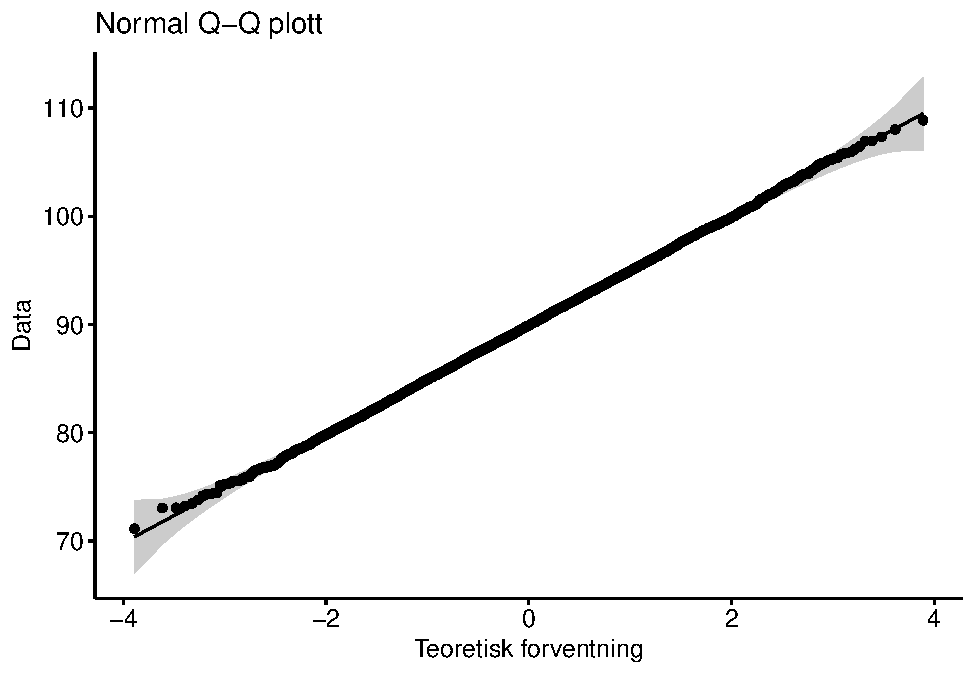
\includegraphics{SPC-book_files/figure-latex/unnamed-chunk-44-1.pdf}
\caption{\label{fig:unnamed-chunk-44}Q-Q plott normalfordeling}
\end{figure}

Vi ser at dette Q-Q plottet viser oss at vi kan være ganske sikre på at dette datasettet er normalfordelt (noe som gir meninig siden vi har brukt R til å lage et normalfordelt datasett).

Tolkning av Q-Q plott er imidlertid ikke alltid så enkelt som i eksempelet ovenfor - det er en viss grad av subjektivitet involvert. Underhar vi gjengitt noen typiske mønstre vi kan se og hva de skyldes. Som et supplement til Q-Q plott kan vi bruke ulike testverdier (fra f.eks. Shapiro-Wilk og Anderson-Darling). Disse kommer vi tilbake til senere i kapittelet.

I det første eksempelet på avvik fra den helt klare normalfordelingen lager vi et datasett som har en skjevhet mot høyre (``right skewness'') - også kalt positiv skjevhet (uten at det legges noe ``positivt'' i positivt). Datasettet kan lastes ned i Excelformat her:

\begin{figure}
\centering
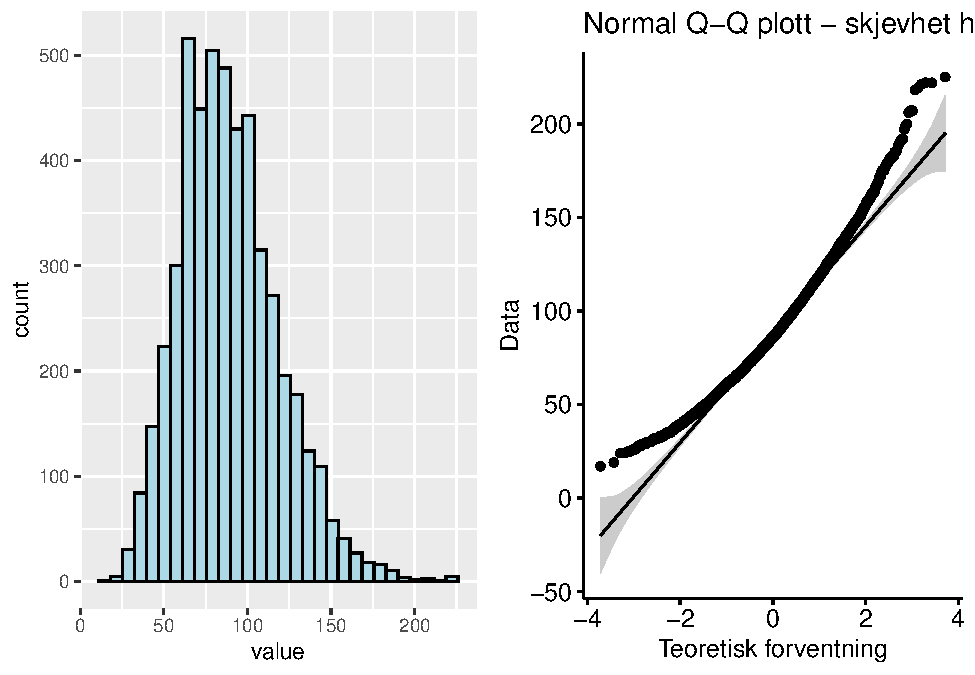
\includegraphics{SPC-book_files/figure-latex/unnamed-chunk-46-1.pdf}
\caption{\label{fig:unnamed-chunk-46}Q-Q plott - fordeling skjevhet høyre}
\end{figure}

I et datasett med høyreskjevhet vil ofte Q-Q plottet vise en bananform med ``bunnen''/midten av bananen ned mot høyre hjørne og endene pekende oppover/utover fra den rette linjen.

I det neste datasettet har vi generert en kraftig skjevhet til venstre. Q-Q plottet får da en omvendt bananform i forhold til høyre skjevhet, altså en topp på midten og to ender som svinger nedover ift den rette linja. Datasettet finner du her:

\begin{figure}
\centering
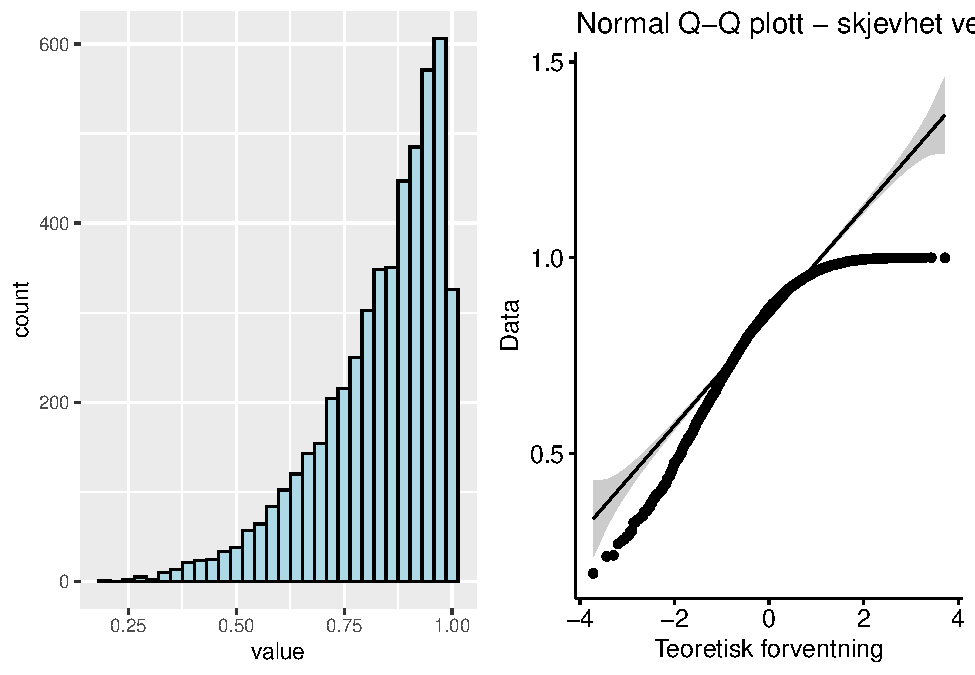
\includegraphics{SPC-book_files/figure-latex/unnamed-chunk-48-1.pdf}
\caption{\label{fig:unnamed-chunk-48}Q-Q plott - fordeling skjevhet venstre}
\end{figure}

De neste to tilfellene av avvik vi skal ta for oss er såkalte ``light-tailed'' (lette haler med liten sannsynlighet for ekstreme verdier og utvalg tendeerer til å ikke fravike gjennomsnittet med mye) og ``heavy-tailed'' (fete/tunge haler med større sannsynlighet for at ekstreme verdier vil forekomme) fordelinger. Datasett for fete haler er her:

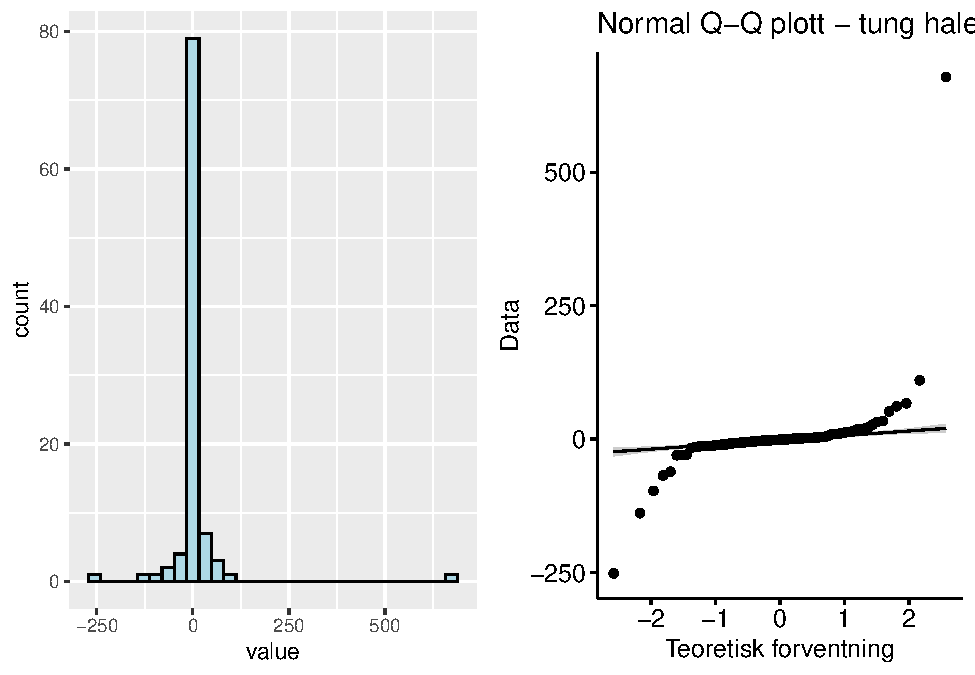
\includegraphics{SPC-book_files/figure-latex/unnamed-chunk-50-1.pdf}
Fordelinger med tunge haler vil ofte følge en slags S-form, men den er ofte mer ``liggende'' enn S-formen til fordeling med lette haler. Den starter med å vokse raskere enn normalfordelingen og ender med å vokse saktere.

Datasettet for lette haler finner du her:

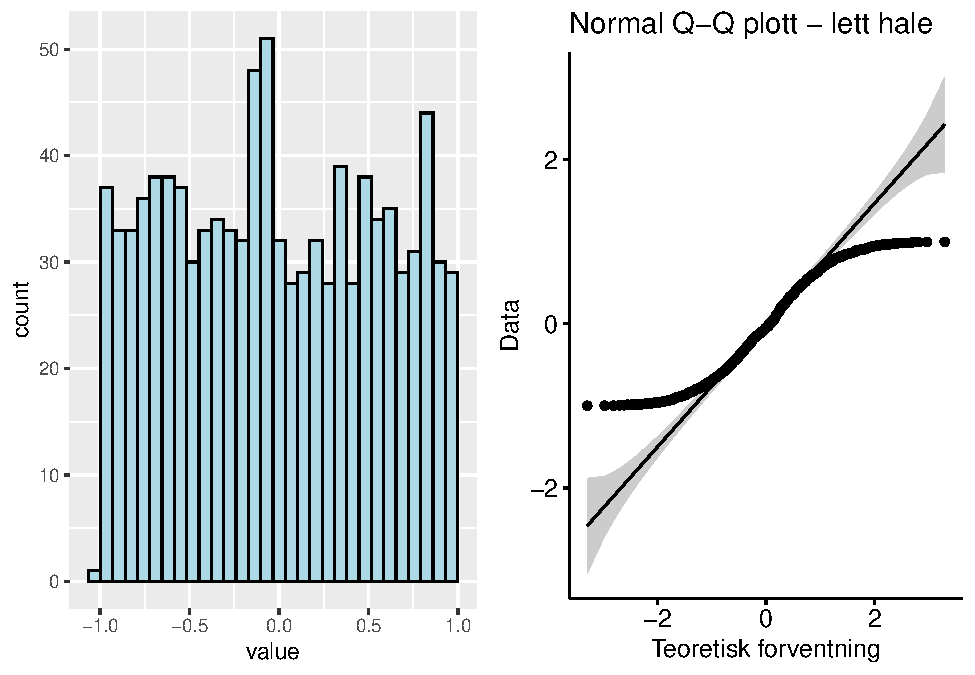
\includegraphics{SPC-book_files/figure-latex/unnamed-chunk-52-1.pdf}
Q-Q plottet for en fordeling med lette haler har ofte en S-form. Dataene vokser saktere enn normalfordelingen i starten før den følger vekstraten til normalfordelingen. Mot slutten vokser den raskere enn normalfordelingen. Derfor bøyer den av fra normalfordelingen.

Til slutt kan vi se på en typisk bimodial fordeling, med datasett her:

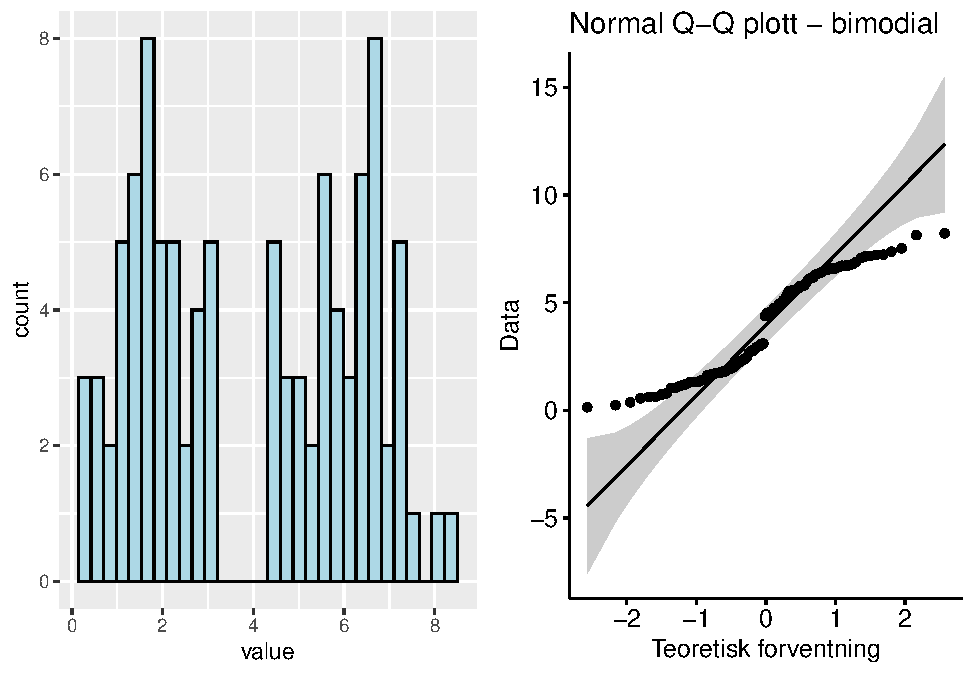
\includegraphics{SPC-book_files/figure-latex/unnamed-chunk-54-1.pdf}
Den bimodiale fordelingen viser ofte et brudd eller et distinkt knekkpunkt rundt krysning av den rette linja, med en del av linja på hver side av den rette linja.

Vi har nå sett på noen typiske eksempler på mønstre i Q-Q plott. Det kan imidlertid være vanskelig å bedømme fordelinger som ligger nære normalfordelingen, men likevel ikke perfekt oppå (du vil trolig aldri se en perfekt match med mindre du har generert et normalfordelt datasett med mange datapunkter). Vi kan supplere Q-Q plottene med visse statistiske tester - det er tema for de neste delkapitlene (men husk: disse statistiske testene har sine egne forutsetninger og er heller ikke uten utfordringer).

\hypertarget{anderson-darling-test-for-normalitet}{%
\section{Anderson-Darling test for normalitet}\label{anderson-darling-test-for-normalitet}}

Anderson-Darlings test er en test for å se om et datasett kommer fra en gitt fordeling, f.eks. normalfordelingen (Anderson and Darling 1954, 1952). Testen setter opp to hypoteser:

\begin{itemize}
\tightlist
\item
  \(H_0\): Dataene følger normalfordelingen
\item
  \(H_1\): Dataene følger ikke normalfordelingen
\end{itemize}

Vi har laget en video (basert på Zaiontz 2020) som viser hvordan du kan gjennomføre en A-D test i Excel som ligger \includegraphics{https://vimeo.com/629254337}. Vi bruker det samme datasettet som i videoen og du kan laste ned datasettet.

Som vi kan se av resultatet fra testen med pakken \textbf{nortest} i R får vi samme verdier som når vi gjør dette manuelt i Excel (jfr video).

\begin{verbatim}
## 
##  Anderson-Darling normality test
## 
## data:  addata$Values
## A = 0.74573, p-value = 0.04046
\end{verbatim}

Siden vi vet at nullhypotesen er at datasettet \textbf{har} en normalfordeling vil vi forkaste nullhypotesen dersom vi har en signifikant p-verdi (grensen for hva som er signifikant bestemmer vi forsåvidt selv, men vanlige verdier er 0.01, 0.05 og 0.1). Altså - i dette tilfellet har vi en p-verdi=0.04. Vi forkaster derfor nullhypotesen og aksepterer \(H_1\) som sier at dataene er trolig ikke er normalfordelte (med andre ord: p-verdien må være større enn signifikansverdien for at vi skal si at dataene trolig er normalfordelte).

I vårt tilfelle ser dette slik ut (Hartmann, Krois, and Waske 2018a):

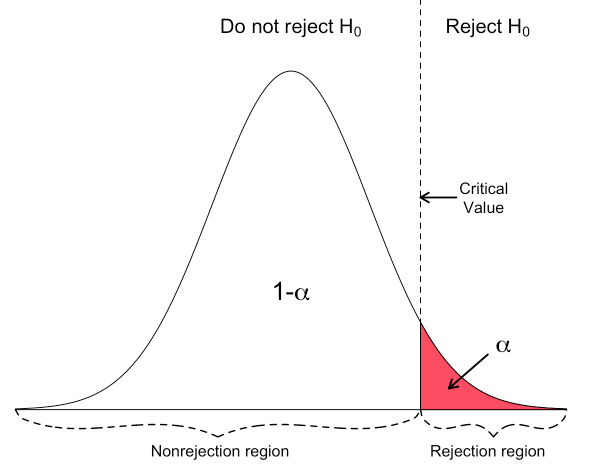
\includegraphics{Hartman1.png}

Det er verdt å merke seg at Anderson-Darling testen egentlig ikke forteller deg at dataene dine er normalfordelte, men at det er usannsynlig at de ikke er det om testen viser det. Dette synes kanskje som samme sak, men er i realiteten en viktig erkjennelse -- en tørr gressplen er et bevis for at det ikke har regnet, men en våt gressplen er ikke bevis for at det har regnet. En våt gressplen kan skyldes andre ting enn regn. Altså -- en signifikant p-verdi på testen gjør at vi forkaster \(H_0\) og antar at fordelingen er ikke-normal. En ikke-signifikant p-verdi på gjør at vi med f.eks. 95\% konfidens kan si at vi ikke har funnet avvik fra normalfordelingen.

Tabellarisk kan vi oppsummere vurderingene slik:

\begin{table}[!h]
\centering
\begin{tabular}{l|l}
\hline
Betingelse & Vurdering\\
\hline
p-verdi $\le$ valgt signifikansnivå & Forkast $H_0$ - datene er trolig ikke normalfordelte\\
\hline
p-verdi > valgt signifikansnivå & Behold $H_0$ - dataene er trolig normalfordelte\\
\hline
Testverdi ($A^2$ verdi) > kritisk verdi & Forkast $H_0$ - datene er trolig ikke normalfordelte\\
\hline
Testverdi ($A^2$ verdi) $\le$ kritisk verdi & Behold $H_0$ - dataene er trolig normalfordelte\\
\hline
\end{tabular}
\end{table}

For at vi skal anta at dataene er normalfordelte må altså p-verdien være større enn valgt signifikansnivå og testverdien være mindre eller lik kritisk verdi. Kritisk verdi leses av i tabell i vedlegg 7. Kritisk verdi referer til det punktet i en teoretisk distribusjon man sammenlikner med en testverdi. Som det framgår av tabellen for kritisk verdi i vedlegget er kritisk verdi låst til valgt signifikansnivå. Kritisk verdi er dermed en terskelverdi for statistisk signifikans -- kritisk verdi svarer på spørsmålet «hvor langt fra gjennomsnittsverdien må du bevege deg for å dekke en gitt andel av variansen i datasettet» (f.eks. 90\%, 95\%, 99\%). Generelt vil man forkaste nullhypotesen dersom testverdien overstiger den kritiske verdien. I vårt eksempel ovenfor fikk vi en A-verdi på 0,74573. Kritisk verdi for 0,05 (95\%) for normalfordeling (vedlegg 7) er 0,752. Her kan man legge merke til at \emph{normtest} pakken i R regner ut A-verdien som er identisk med den A-verdien vi viser i Excelvideoen. Imidlertid gjøres det ofte en korreksjon for sammenlikning med normalfordeling (korreksjoner for ulike fordelinger, jfr vedlegg 7) slik at man får en A\^{}2 verdi. Den har vi i Excel regnet ut til 0,7904. For vår vurdering blir dette viktig - bruker vi A-verdien får vi et forvirrende resultat, der p-verdien sier vi ikke har et normalfordelt datasett. A-verdien er mindre enn kritisk verdi så den indikerer at dataene er normalfordelte, mens A\^{}2-verdien er større og indikerer at de ikke er normalfordelte. Vi må anta at A\^{}2-verdien er mer korrekt, og til slutt konkludere med at vi tror dataene ikke er normalfordelte.

Vi kan se på et Q-Q plott for dette datasettet også:
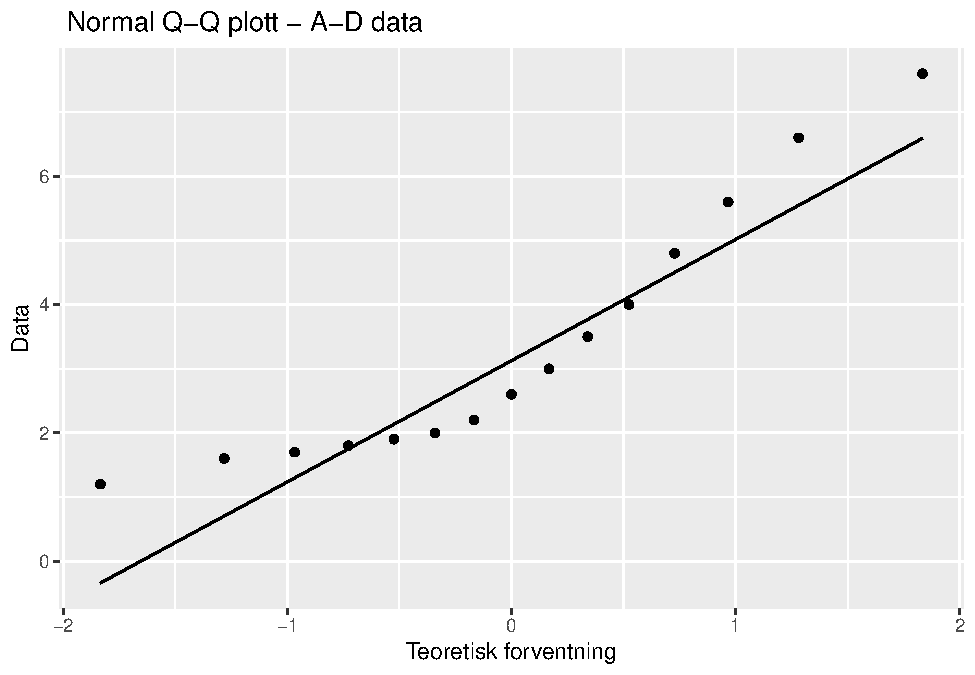
\includegraphics{SPC-book_files/figure-latex/unnamed-chunk-58-1.pdf}
Q-Q plottet støtter vår vurdering om at dette datasettet ikke er normalfordelt. Når det gjelder A-D testen skal vi altså være oppmerksom på om programmet vi bruker regner ut den generiske A-verdien eller den mer korrekt A\^{}2-verdien (dersom vi tester for normalfordeling).

Hvis vi bruker \emph{normtest} på det vi vet er et normalfordelt datasett (jfr vårt første eksempel på et Q-Q plott i dette kapittelet) får vi:

\begin{verbatim}
## 
##  Anderson-Darling normality test
## 
## data:  addata4$value
## A = 0.15306, p-value = 0.9591
\end{verbatim}

Her ser vi, ikke overraskende, at både p-verdi og kritisk verdi tilsier at datasettet er normalfordelt.

Det finnes flere andre statistiske tester som kan kjøres for å teste for normalitet, f.eks. Kologorov-Smirnov, Shapiro-Wilks og Cramer Von-Mises test. Vi går ikke inn på manuell utregning av disse i Excel. Anderson-Darling er en modifisering/videreutvikling av Kolmogorov-Smirnov (Guthrie 2020) og anses ofte som en bedre test.For sammenlikningens skyld kjører vi disse i R:

\begin{verbatim}
## 
##  One-sample Kolmogorov-Smirnov test
## 
## data:  addata5
## D = 0.88493, p-value = 0.0000000000000171
## alternative hypothesis: two-sided
\end{verbatim}

\begin{verbatim}
## 
##  Shapiro-Wilk normality test
## 
## data:  addata5$Values
## W = 0.87521, p-value = 0.04027
\end{verbatim}

\begin{verbatim}
## 
##  Cramer-von Mises normality test
## 
## data:  addata$Values
## W = 0.12634, p-value = 0.04326
\end{verbatim}

Tolkning Kolmogorov-Smirnov: Hvis p-verdien er under valgte signifikansnivå (f.eks. 0.05) skal vi anta at datasettet ikke er normalfordelt. Her vil testen peke på at datasettet \emph{ikke} er normalfordelt.

Tolkning av Shapiro-Wilks og Cramer-von Mieses test er lik som for Kolmogorov-Smirnov.

Som et siste eksempel på en statistisk test for normalitet kan vi bruke Jarque-Bera test. Denne skiller seg litt ut fra de andre ved at den spesifikt ser på skjevhet og kurtosis i datasettet opp mot hva en normalfordeling vil ha. For å gjøre lykken komplett finnes det versjoner av testen:

\begin{verbatim}
## 
##  Jarque Bera Test
## 
## data:  addata6$Values
## X-squared = 2.1953, df = 2, p-value = 0.3337
\end{verbatim}

\begin{verbatim}
## 
##  Adjusted Jarque-Bera test for normality
## 
## data:  addata6$Values
## AJB = 3.1014, p-value = 0.131
\end{verbatim}

Tolkningen er lik som før - hvis p-verdien er mindre enn valgte signifikansnivå peker det mot at datasettet ikke er normalfordelt. Her, i motsetning til de øvrige testene, er p-verdien større enn signifikansnivået (0,05) så det peker mot at datasettet \emph{er} normalfordelt.

Dette er altså ikke så enkelt. Det finnes mange statistiske tester, som kan gi motsatte indikasjoner på om et datasett er normalfordelt eller ikke. Vårt råd blir: Start alltid med Q-Q plott. Velg evt en teststatistikk, men vær klar over at alle teststatistikker bygger på forutsetninger eller tester ulike sider av distribusjonen. Det vi også kan huske på er at i henhold til sentralgrenseteoremet (``Central Limit Theorem'') - se vedlegg 4 - vil populasjonens fordeling være av mindre interesse dersom utvalgsstørrelsen er stor nok. Hva er stor nok? De fleste kilder peker mot at over 30 er ``stort nok.''

En siste ting for å gjøre forvirringen komplett\ldots{} Vi kan ta det opprinnelige Q-Q plottet for dette datasettet og legge på konfidensintervaller:

\begin{figure}
\centering
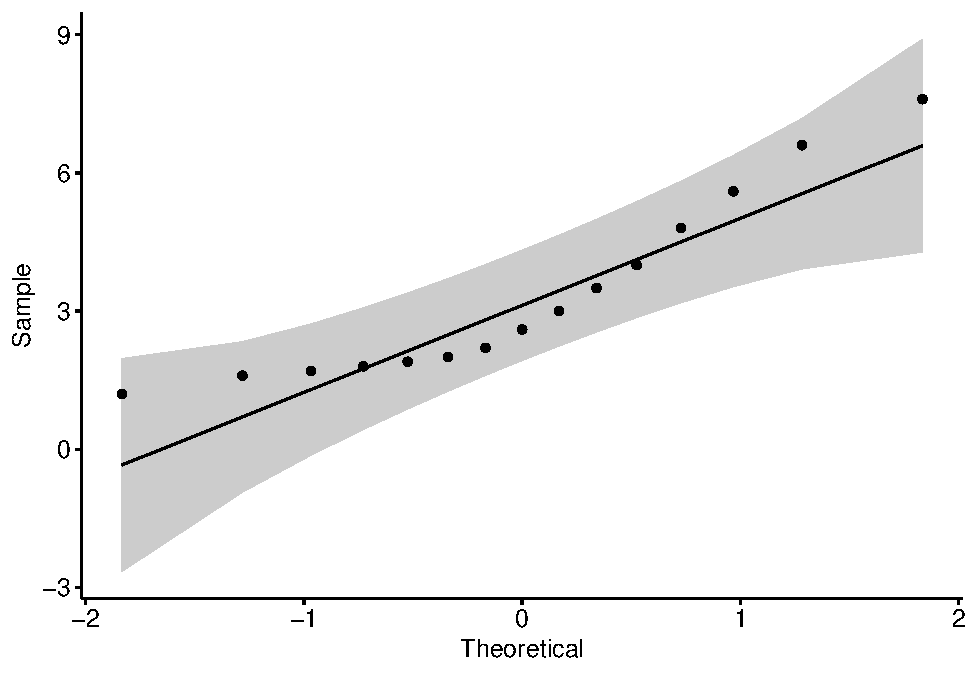
\includegraphics{SPC-book_files/figure-latex/unnamed-chunk-62-1.pdf}
\caption{\label{fig:unnamed-chunk-62}Q-Q plott - med konfidensgrenser}
\end{figure}

Tolkningen er: Dersom Q-Q plottpunktene i all hovedsak ligger innenfor konfidensintervallene (på figuren over markert med grå farge) er dataene ``sånn ca. normalfordelte.'' Vi går ikke nærmere inn på begrepet konfidensintervaller her ut over å si at konfidensintervaller sier noe om gode estimater er. Datasettet vårt er et utvalg. Dette utvalget sammenlikner vi med datafordelingen til et normalfordelt datasett i et Q-Q plott. Q-Q plottet sier oss da, som vi nå vet, noe om vårt datasett og et normalfordelt datasett er like. Dersom vi hypotetisk sett tar uendelig mange utvalg slik vi har fått vårt datasett så kan vi med 95\% sikkerhet\footnote{Gitt at vi har valgt 5\% signifikansnivå} si at Q-Q plottdatapunktene vil falle innenfor grensene. Husk at et Q-Q plott ikke er en test for å se om dataene er normalfordelte, men en sjekk om dataene har synlige avvik fra normalfordelingen.

\hypertarget{seriediagram}{%
\chapter{Seriediagram}\label{seriediagram}}

Den første analysen vi gir oss i kast med etter å ha fått en forståelse av dataene våre er et seriediagram. Et seriediagram (jfr. Anhøj and Bjørn 2009) (ofte referert til som ``run diagram'' siden dette er den engelske betegnelsen)\footnote{I norsk litteratur og nettsteder brukes ofte betegnelsen «run diagram» (se f.eks. Brudvik (2009)). Selv om vi ikke har noe religiøst forhold til å finne norske begreper på ethvert engelsk begrep mener vi likevel begrepet seriediagram er et mer intuitivt begrep enn «run diagram».Selv om vi ikke har noe religiøst forhold til å finne norske begreper på ethvert engelsk begrep mener vi likevel begrepet seriediagram er et mer intuitivt begrep enn «run diagram».} er en framstilling av en serie hendelser sekvensielt i tid. Et seriediagram er enkelt å konstruere og tolke. I dette diagrammet kan vi bruke både måledata og telledata, og det spiller ingen rolle om det er hendelser, prosenter eller andeler (i kontrolldiagrammer vil vi være nøye med å skille mellom hvilke typer data vi har slik at vi velger rett kontrolldiagram). Den eneste forutsetningen vi må ha med oss for seriediagrammer er at punktene er uavhengige, altså at verdien i et punkt ikke er påvirket av verdien på foregående punkt. I tillegg anbefales minst 10 punkter av Berardinelli and Yerian (n.d.), 15 punkter (Reynolds et al. 2021), mens Anhøj and Bjørn (2009) anbefaler mellom 20 og 30 datapunkter for å få et robust seriediagram. Anbefalingen på mellom 20 og 30 hviler på en balanse mellom å se unormal variasjon der prosessen egentlig er stabil (såkalt type-1 feil) og å ikke se unormal variasjon der den faktisk finnes (såkalt type-2 feil). Det er derfor verdt å merke seg at «mer ikke er bedre» - et stort antall datapunkter øker ikke den statistiske styrken, men øker sjansen for type-2 feil. Vi legger til grunn at anbefalingen fra Anhøj and Bjørn (2009) virker godt fundert.

Et seriediagram vil kunne vise oss noe om variasjon, men vi kan også gå glipp av noen mer spesielle former for variasjon. Så fordelen i enkelheten må veies opp mot ulempen ved å være litt mindre sensitiv for spesiell variasjon. Plottingen av et seriediagram kan gjøres enkelt med penn og papir ved at man tiden på x-aksen og en verdi av en måling, en observasjon e.l. på y-aksen. Deretter forbinder man punktene med en linje, og legger til medianen (som er verdien av det datapunktet som deler et utvalg i to)\footnote{Har man en serie med oddetall observasjoner vil medianverdien utgjøres av et punkt, mens om man har et partall observasjoner utgjør gjennomsnittet av de to nærmest midten medianverdien.}.

Hvorfor «serie» (``run'')? En serie er i denne sammenhengen definert som et antall (ett eller flere) punkter i diagrammet på samme side av medianen. I diagrammet under ser vi et eksempel på et seriediagram. Vi plotter ganske enkelt inn hver enkelt observasjon fortløpende i tid utover x-aksen og verdien iht y-aksen. Sentraltendensen er medianen, hvilket innebærer at halvparten av målingene er over og halve under medianstreken.

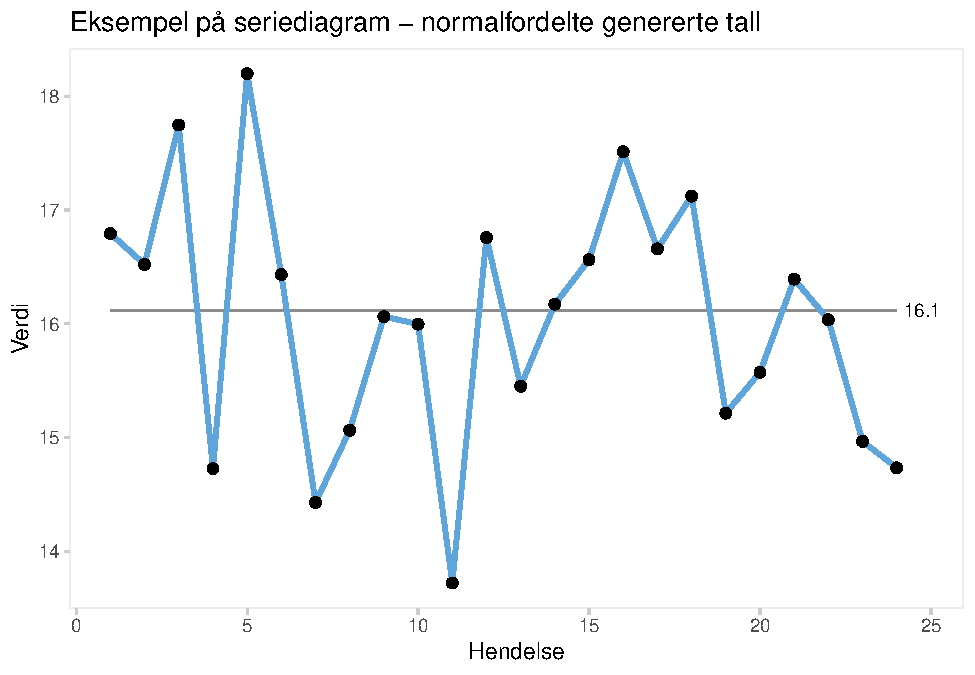
\includegraphics{SPC-book_files/figure-latex/unnamed-chunk-63-1.pdf}
Når vi skal tolke seriediagrammet finnes det flere sett av retningslinjer, f.eks. gitt av Carey (2002) og Perla, Provost, and Murray (2011). Vi velger å bruke «Anhøj-reglene» (Anhøj 2015; Anhøj and Wentzel-Larsen 2020) på seriediagrammene. For det første er det vist at disse reglene gir en god balanse mellom type-1 og type-2 feil. For det andre er det to enkle regler å forholde seg til som gjør tolkningen enklere og raskere. Anhøj-reglene ser på to forhold:

\begin{enumerate}
\def\labelenumi{\arabic{enumi}.}
\tightlist
\item
  Uvanlig lange serier. Her kan man matematisk regne ut hvor lang serien må være for å regnes som «uvanlig lang»: \(log2(n)\) der n = antall punkter/hendelser (Anhøj 2015). Så for eksempelet ovenfor må serien være \(log2(30)+3=8\). Det innebærer at dersom vi har flere enn 8 datapunkter etter hverandre på samme side av senterlinjen vil indikere et skift i prosessen.
\item
  Uvanlig få krysninger av senterlinjen. Også her kan vi regne ut hvor mange krysningspunkter det bør være \(b(n-1.05)\)\footnote{I en prosess som er tilfeldig vil det være 50-50 sjanse for å krysse medianlinjen mellom to punkter som kommer etter hverandre. Det totale antallet krysninger har således en binomialfordeling (Anhøj 2015)}. For eksempelet ovenfor blir derfor et minimum antall krysningspunkter 8. Færre enn 8 krysningspunkter vil indikere et skift i prosessen.
\end{enumerate}

Heldigvis kan det settes opp en tabell slik at vi enkelt kan lese ut de kritiske verdiene (Anhøj and Wentzel-Larsen 2020) (se vedlegg 2). I eksempelet under har vi igjen 24 observasjoner. Vi bør forvente minst 8 krysninger (regel 2) og siden vi har flere punkter enn 8 etter hverandre på samme side (regel 1) har vi brudd på begge reglene. Dette indikerer en prosess ute av kontroll med unormal variasjon.

I et nytt eksempel kan vi provosere fram brudd på Anhøj-reglene:

\begin{figure}
\centering
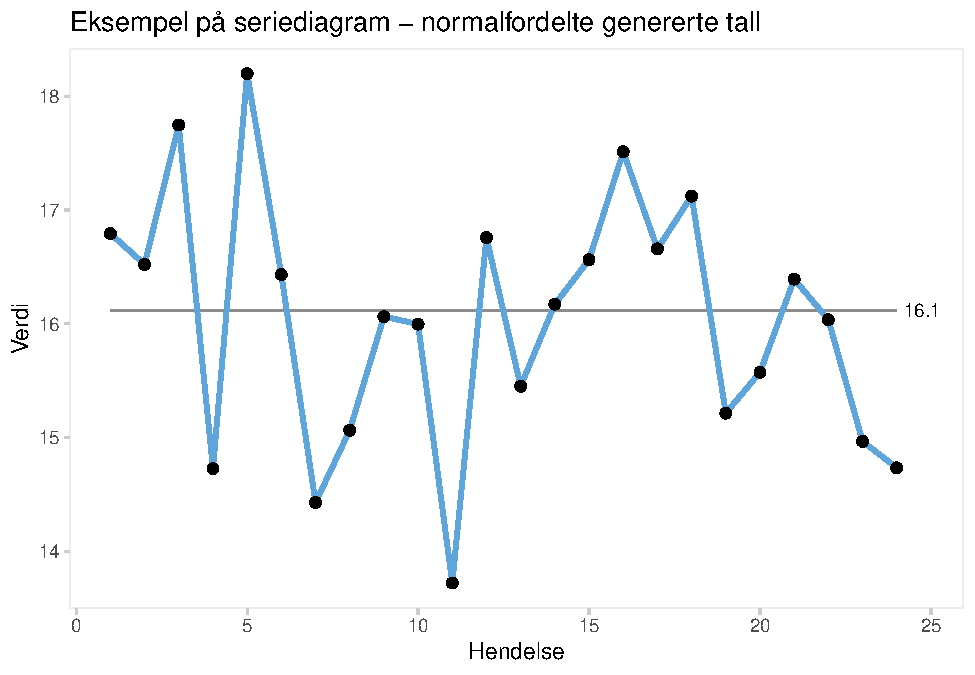
\includegraphics{SPC-book_files/figure-latex/unnamed-chunk-64-1.pdf}
\caption{\label{fig:unnamed-chunk-64}Eksempel seriediagram - modifiserte tall}
\end{figure}

I det modifiserte seriediagrammet har vi like mange punkter som det forrige (24) så vi burde forvente minst 8 krysninger (regel 2) og siden vi har flere punkter enn 8 etter hverandre på samme side (regel 1) har vi brudd på begge reglene. Dette indikerer en prosess ute av kontroll med unormal variasjon.

Man må imidlertid være observant på eventuelle endringer i prosesser. I eksempelet ovenfor kan man tenke seg en prosessendring etter hendelse 15. Hvis vi legger dette så vi får et brudd i dataserien etter hendelse 15 inn får vi et annet bilde:

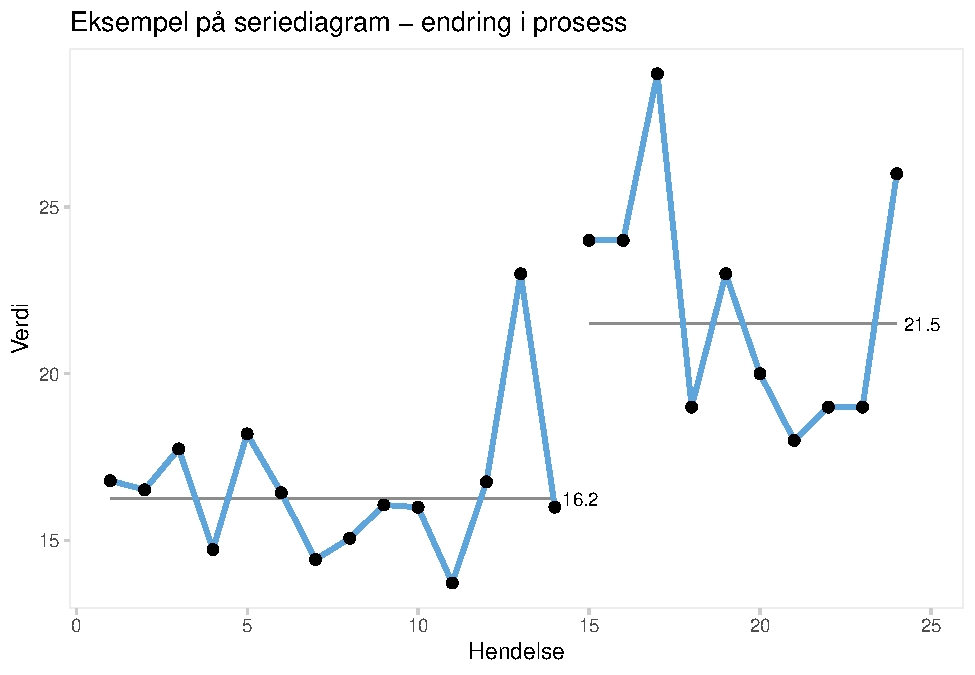
\includegraphics{SPC-book_files/figure-latex/unnamed-chunk-65-1.pdf}
I første del av prosessen har vi 14 punkter. Iht vedlegg 2 bør vi da ha minst 4 krysninger og maks 7 punkter på samme side for å få en serie. I andre del har vi 10 punkter. Da skal vi ha minst 2 krysninger og maks 6 punkter på samme side. Ingen av de to delene bryter med Anhøjs regler.

Gjennom sin enkelhet vil et seriediagram kunne spare oss for unødvendig arbeid med kontrolldiagrammer (se neste avsnitt). Hvis vi har tegn på unormal variasjon i et seriediagram vil det være liten grunn til å utvikle kontrolldiagram da vi allerede i seriediagrammet kan konstatere unormal variasjon. Tvert imot, som Anhøj (2009) påpeker, kan utviklingen av kontrolldiagrammer være påvirket av tilstedeværelsen av unormal variasjon ved at beregningen av kontrollparameterne gjennomsnitt og kontrollgrenser blir uforutsigbar. Det kan derfor være et godt tips å starte med et seriediagram, tolke det og deretter bestemme seg for hvordan man går videre.

Som Anhøj (2021a) uttrykker det: ``It is a common misunderstanding that control charts are superior to run charts. The confusion may stem from the fact that different sets of rules for identifying non-random variation in run charts are available, and that these sets differ significantly in their diagnostic properties.'' Og videre: ``One big advantage of run charts is that they are oblivious to assumptions on the theoretical distribution of data. Also they are easier to construct (by pen and paper) and understand than are control charts. Finally, as mentioned, the diagnostic value of run charts is independent of the number of data points, which is not the case with control charts unless one adjusts the control limits in accordance with the number of data points.In practice I always do the run chart analysis first. If, and only if, the run chart shows random variation and I need to further investigate data for outliers or to know the limits of common cause variation, I would do a control chart analysis\ldots{}''

Anhøj (2021a) påpker imidlertid et viktig unntak fra tilnærmingen om å alltid se på et seriediagram først: Om man har sjeldne data bør man heller lage et g eller t kontrolldiagram (se neste kapittel) siden seriediagram er dårlig egnet til å detektere endringer i disse tilfellene.

Vi vil derfor avslutte dette kapittelet med å \textbf{sterkt} anbefale at man begynner med et seriediagram.

Balestracci (2014):

\begin{quote}
``Over the years, I have developed an increasing affection for the much-neglected run chart: a time plot of your process data with the median drawn in as a reference (yes, the median---not the average). It is''filter No.~1" for any process data and answers the question: ``Did this process have at least one shift during this time period?'' (This is generally signaled by a clump of eight consecutive data points either all above or below the median.)
If it did, then it makes no sense to do a control chart at this time because the overall average of all these data doesn't exist. (Sort of like: If I put my right foot in a bucket of boiling water and my left foot in a bucket of ice water, on average, I'm pretty comfortable.)"
\end{quote}

\hypertarget{kontrolldiagram}{%
\chapter{Kontrolldiagram}\label{kontrolldiagram}}

Et kontrolldiagram er mer sensitivt for å vise spesielle typer variasjon enn et run diagram. For å oppnå denne økte sensitiviteten er det imidlertid viktig at man velger riktig type kontrolldiagram ut fra hvilken type data man har. Her vil flytdiagrammet på s.xxxx kunne være til hjelp for å velge riktig type, men vi vil også gå gjennom hvert enkelt kontrolldiagram nedenfor. Man skal imidlertid ikke anta at et seriediagram er «mindre verdt» enn et kontrolldiagram. Selv om kontrolldiagram er mer sensitive ovenfor spesielle typer variasjon, er seriediagram mer sensitive ovenfor mindre skifter i dataene (under 2 SD) enn kontrolldiagrammene som typisk reagerer på større skifter i dataene (rundt 2 SD og mer) (Anhøj and Olesen 2014). Et seriediagram kan derfor ofte være et viktig første steg før man tar i bruk mer sofistikerte verktøy som kontrolldiagram (Perla, Provost, and Murray 2011).

En spesiell egenskap ved kontrolldiagram er at den kan hjelpe oss til å se yteevnen til en stabil prosess. Med det mener vi hvilke grenser prosessen trolig vil holde seg innenfor. Dette kalles ofte for prosesskapabilitet. Dette vil vi komme nærmere tilbake til i et senere avsnitt.

Så hva er et kontrolldiagram? Et kontrolldiagram er en statistisk tilnærming til å se på prosesser, variasjon i prosesser og om prosesser produserer resultater innenfor gitte akseptable grenser. Det likner på i stor grad på et seriediagram. Vi plotter inn en rekke hendelser eller observasjoner i et diagram der tiden for observasjonene plottes fortløpende i tid på x-aksen og verdien eller antall hendelser på y-aksen. Det et kontrolldiagram tilfører er at det inkluderer mer avanserte analyser gjennom å regne ut to kontrollgrenser som lar oss vurdere statistisk etter andre regler enn seriediagrammet om en prosess har normal eller unormal variasjon. I tillegg er kontrolldiagrammene basert på at sentraltendensen er gjennomsnittet, ikke median (som i seriediagrammet).

Shewhart baserte sin tilnærming til kontrolldiagram på matematisk teori (se vedlegg 7 for forklaring på Chebyshevs teorem) og egne empiriske erfaringer når han satt verdiene for øvre og nedre kontrollgrenser til tre sigma (tre standardavvik). Flere tiårs erfaring fra en lang rekke områder viser at tre sigma som grenseverdier holder vann (M. A. Mohammed, Worthington, and Woodall 2008).

Et kontrolldiagram kan se slik ut (R pakken \emph{qicharts2} (Anhøj 2020):
\includegraphics{SPC-book_files/figure-latex/unnamed-chunk-66-1.pdf}
Observasjonene/målingene plottes som punkter sekvensielt i tid. Snittet er -0,2, UCL 2,2 og LCL -2,7.

Tilsvarende data ved bruk av R pakken \emph{qcc} (Scrucca, Snow, and Bloomfield 2017):
\includegraphics{SPC-book_files/figure-latex/unnamed-chunk-67-1.pdf}

Alle kontrolldiagram vil ha tre horisontale linjer: En gjennomsnittsverdi, en øvre kontrollgrense og en nedre kontrollgrense (øvre og nedre kontrollgrense kan ved enkelte typer kontrolldiagram avvike fra en ren horisontal linje, men ha et horisontalt mønster.

Ulike programmer eller R-pakker gir ulik grafisk framstilling.Analyse-It i Excel gir dette for samme data:

\includegraphics{Eks_kontrdiagr.png}

Vi skal også være oppmerksom på at de kan opererer med ulike ``regler'' for når de flagger unormal variasjon. Ulike programmer kan imidlertid ha lagt inn noe ulike regler for hva som betraktes som unormal variasjon. Det er derfor lurt å sette seg inn i hvilke regler som benyttes i det programmet du bruker -- alle programmene vil, på en eller annen måte, indikere unormal variasjon hvis vi ber programmet om å gjøre det. Og de fleste programmene vil også la oss velge mellom hvilke kontrollregler vi ønsker å bruke. Her må man altså sjekke opp ut fra hvilket program/R-pakke man ønsker å bruke. I det videre vil vi i hovedsak bruke \emph{qcc} og \emph{qicharts2}. Ulike sett regler har vokst fram fra det som regnes som de opprinnelige 4 reglene (1, 2, 5 og 6) (Western Electric Company 1956), til Nelson (1984) 8 regler som er modifisert av flere, blant annet Montgomery (2020) (som \emph{qicharts2} bruker).Pakken \emph{qcc} bruker reglene 1, 2, 3 og 4 som ``Shewhart reglene.''

\providecommand{\docline}[3]{\noalign{\global\setlength{\arrayrulewidth}{#1}}\arrayrulecolor[HTML]{#2}\cline{#3}}

\setlength{\tabcolsep}{2pt}

\renewcommand*{\arraystretch}{1.5}

\begin{longtable}[c]{ccc}



\hhline{>{\arrayrulecolor[HTML]{666666}\global\arrayrulewidth=2pt}->{\arrayrulecolor[HTML]{666666}\global\arrayrulewidth=2pt}->{\arrayrulecolor[HTML]{666666}\global\arrayrulewidth=2pt}-}

\multicolumn{1}{!{\color[HTML]{000000}\vrule width 0pt}>{}l}{\fontsize{11}{11}\selectfont{\textcolor[HTML]{000000}{Test}}} & \multicolumn{1}{!{\color[HTML]{000000}\vrule width 0pt}>{}l}{\fontsize{11}{11}\selectfont{\textcolor[HTML]{000000}{Regel}}} & \multicolumn{1}{!{\color[HTML]{000000}\vrule width 0pt}>{}l!{\color[HTML]{000000}\vrule width 0pt}}{\fontsize{11}{11}\selectfont{\textcolor[HTML]{000000}{Indikasjon}}} \\

\hhline{>{\arrayrulecolor[HTML]{666666}\global\arrayrulewidth=2pt}->{\arrayrulecolor[HTML]{666666}\global\arrayrulewidth=2pt}->{\arrayrulecolor[HTML]{666666}\global\arrayrulewidth=2pt}-}

\endfirsthead

\hhline{>{\arrayrulecolor[HTML]{666666}\global\arrayrulewidth=2pt}->{\arrayrulecolor[HTML]{666666}\global\arrayrulewidth=2pt}->{\arrayrulecolor[HTML]{666666}\global\arrayrulewidth=2pt}-}

\multicolumn{1}{!{\color[HTML]{000000}\vrule width 0pt}>{}l}{\fontsize{11}{11}\selectfont{\textcolor[HTML]{000000}{Test}}} & \multicolumn{1}{!{\color[HTML]{000000}\vrule width 0pt}>{}l}{\fontsize{11}{11}\selectfont{\textcolor[HTML]{000000}{Regel}}} & \multicolumn{1}{!{\color[HTML]{000000}\vrule width 0pt}>{}l!{\color[HTML]{000000}\vrule width 0pt}}{\fontsize{11}{11}\selectfont{\textcolor[HTML]{000000}{Indikasjon}}} \\

\hhline{>{\arrayrulecolor[HTML]{666666}\global\arrayrulewidth=2pt}->{\arrayrulecolor[HTML]{666666}\global\arrayrulewidth=2pt}->{\arrayrulecolor[HTML]{666666}\global\arrayrulewidth=2pt}-}\endhead



\multicolumn{1}{!{\color[HTML]{000000}\vrule width 0pt}>{}l}{\fontsize{11}{11}\selectfont{\textcolor[HTML]{000000}{1}}} & \multicolumn{1}{!{\color[HTML]{000000}\vrule width 0pt}>{}l}{\fontsize{11}{11}\selectfont{\textcolor[HTML]{000000}{1\ punkt\ utenfor\ kontrollgrensene}}} & \multicolumn{1}{!{\color[HTML]{000000}\vrule width 0pt}>{}l!{\color[HTML]{000000}\vrule width 0pt}}{\fontsize{11}{11}\selectfont{\textcolor[HTML]{000000}{En\ større\ endring}}} \\





\multicolumn{1}{!{\color[HTML]{000000}\vrule width 0pt}>{}l}{\fontsize{11}{11}\selectfont{\textcolor[HTML]{000000}{2}}} & \multicolumn{1}{!{\color[HTML]{000000}\vrule width 0pt}>{}l}{\fontsize{11}{11}\selectfont{\textcolor[HTML]{000000}{2\ av\ 3\ påfølgende\ punkter\ er\ mer\ enn\ 2\ sigma\ fra\ gjennomsnittsverdien\ og\ i\ samme\ retning}}} & \multicolumn{1}{!{\color[HTML]{000000}\vrule width 0pt}>{}l!{\color[HTML]{000000}\vrule width 0pt}}{\fontsize{11}{11}\selectfont{\textcolor[HTML]{000000}{En\ mindre,\ men\ vedvarende\ endring}}} \\





\multicolumn{1}{!{\color[HTML]{000000}\vrule width 0pt}>{}l}{\fontsize{11}{11}\selectfont{\textcolor[HTML]{000000}{3}}} & \multicolumn{1}{!{\color[HTML]{000000}\vrule width 0pt}>{}l}{\fontsize{11}{11}\selectfont{\textcolor[HTML]{000000}{4\ av\ 5\ påfølgende\ punkter\ er\ mer\ enn\ 1\ sigma\ fra\ gjennomsnittsverdien\ og\ i\ samme\ retning}}} & \multicolumn{1}{!{\color[HTML]{000000}\vrule width 0pt}>{}l!{\color[HTML]{000000}\vrule width 0pt}}{\fontsize{11}{11}\selectfont{\textcolor[HTML]{000000}{En\ mindre,\ men\ vedvarende\ endring}}} \\





\multicolumn{1}{!{\color[HTML]{000000}\vrule width 0pt}>{}l}{\fontsize{11}{11}\selectfont{\textcolor[HTML]{000000}{4}}} & \multicolumn{1}{!{\color[HTML]{000000}\vrule width 0pt}>{}l}{\fontsize{11}{11}\selectfont{\textcolor[HTML]{000000}{8\ påfølgende\ punkter\ er\ på\ samme\ side\ av\ gjennomsnittet}}} & \multicolumn{1}{!{\color[HTML]{000000}\vrule width 0pt}>{}l!{\color[HTML]{000000}\vrule width 0pt}}{\fontsize{11}{11}\selectfont{\textcolor[HTML]{000000}{Ikke-tilfeldig\ systematisk\ variasjon}}} \\





\multicolumn{1}{!{\color[HTML]{000000}\vrule width 0pt}>{}l}{\fontsize{11}{11}\selectfont{\textcolor[HTML]{000000}{5}}} & \multicolumn{1}{!{\color[HTML]{000000}\vrule width 0pt}>{}l}{\fontsize{11}{11}\selectfont{\textcolor[HTML]{000000}{6\ påfølgende\ punkter\ er\ i\ stigende\ eller\ synkende\ trend\ (etter\ hverandre)}}} & \multicolumn{1}{!{\color[HTML]{000000}\vrule width 0pt}>{}l!{\color[HTML]{000000}\vrule width 0pt}}{\fontsize{11}{11}\selectfont{\textcolor[HTML]{000000}{En\ middels\ endring}}} \\





\multicolumn{1}{!{\color[HTML]{000000}\vrule width 0pt}>{}l}{\fontsize{11}{11}\selectfont{\textcolor[HTML]{000000}{6}}} & \multicolumn{1}{!{\color[HTML]{000000}\vrule width 0pt}>{}l}{\fontsize{11}{11}\selectfont{\textcolor[HTML]{000000}{15\ påfølgende\ punkter\ er\ innenfor\ +/-\ 1\ sigma\ fra\ gjennomsnittet}}} & \multicolumn{1}{!{\color[HTML]{000000}\vrule width 0pt}>{}l!{\color[HTML]{000000}\vrule width 0pt}}{\fontsize{11}{11}\selectfont{\textcolor[HTML]{000000}{En\ liten\ endring}}} \\





\multicolumn{1}{!{\color[HTML]{000000}\vrule width 0pt}>{}l}{\fontsize{11}{11}\selectfont{\textcolor[HTML]{000000}{7}}} & \multicolumn{1}{!{\color[HTML]{000000}\vrule width 0pt}>{}l}{\fontsize{11}{11}\selectfont{\textcolor[HTML]{000000}{14\ påfølgende\ punkter\ alternerer\ opp\ og\ ned\ (annenhver\ opp\ og\ ned\ i\ forhold\ til\ foregående\ verdi)}}} & \multicolumn{1}{!{\color[HTML]{000000}\vrule width 0pt}>{}l!{\color[HTML]{000000}\vrule width 0pt}}{\fontsize{11}{11}\selectfont{\textcolor[HTML]{000000}{Stratifisering\ (at\ vi\ egentlig\ har\ to\ eller\ flere\ prosesser\ –\ et\ histogram\ vil\ f.eks.\ kunne\ vise\ en\ bimodal\ distribusjon)}}} \\





\multicolumn{1}{!{\color[HTML]{000000}\vrule width 0pt}>{}l}{\fontsize{11}{11}\selectfont{\textcolor[HTML]{000000}{8}}} & \multicolumn{1}{!{\color[HTML]{000000}\vrule width 0pt}>{}l}{\fontsize{11}{11}\selectfont{\textcolor[HTML]{000000}{8\ påfølgende\ punkter\ på\ samme\ side\ av\ gjennomsnittet\ og\ ingen\ innenfor\ +/-\ 1\ sigma}}} & \multicolumn{1}{!{\color[HTML]{000000}\vrule width 0pt}>{}l!{\color[HTML]{000000}\vrule width 0pt}}{\fontsize{11}{11}\selectfont{\textcolor[HTML]{000000}{Blandet\ variasjon}}} \\

\hhline{>{\arrayrulecolor[HTML]{666666}\global\arrayrulewidth=2pt}->{\arrayrulecolor[HTML]{666666}\global\arrayrulewidth=2pt}->{\arrayrulecolor[HTML]{666666}\global\arrayrulewidth=2pt}-}



\end{longtable}

Bruk av regel 1 på en normalfordelte data vil kunne gi «falsk alarm» (vise unormal variasjon når det ikke finnes) i 1 av 370 tilfeller i gjennomsnitt. Hvis man imidlertid legger til testene 2, 5 og 6 stiger raten av feil alarmer til 1 av 91,75 tilfeller. Et godt råd som ofte gis er å velge tester før man lage kontrolldiagrammene basert på kjennskap til prosessen man holder på med. Som Anhøj (2021a) påpeker: ``It is a common misunderstanding that control charts are superior to run charts. The confusion may stem from the fact that different sets of rules for identifying non-random variation in run charts are available, and that these sets differ significantly in their diagnostic properties.''

Eksempel på kontrolldiagram med indikasjon på et eller flere brudd på regler for normal variasjon:

\begin{figure}
\centering
\includegraphics{SPC-book_files/figure-latex/unnamed-chunk-69-1.pdf}
\caption{\label{fig:unnamed-chunk-69}Oversikt regler kontrolldiagram}
\end{figure}

Vi skal i videre i dette kapittelet ta for oss ulike typer kontrolldiagrammene (ref. flytskjema for valg av kontrolldiagram). Vi vil vise et eksempel på hvert av de vanlige kontrolldiagrammene. For hvert eksempel finnes det en Excelfil med dataene som er brukt for de ulike eksemplene og en video som viser framgangsmåten i Excel. Grunnen til dette er at for mange vil Excel være et mye mer kjent grensesnitt enn R. Samtidig, ved å se på videoen og stegene som gjøres, ser man hvordan det enkelte kontrolldiagram er bygd opp. Selvsagt er dette mye mer tidkrevende enn å bare kjøre analysen i R, men det kan gi en fin innsikt i ``hva som egentlig skjer.'' På sikt mener vi det er mye å hente på å bruke R og pakken \emph{qicharts2} eller pakken \emph{qcc}. Alternativt kan man investere i et tillegg til Excel som nevnt i kapittel 1.

\hypertarget{telledata-attributter}{%
\section{Telledata (attributter)}\label{telledata-attributter}}

Diagrammene i dette delkapittelet handler om data der vi kan telle og putte dataene inn i kategorier. Motsetningen er måledata som er kontinuerlige data som behandles i neste delkapittel.

\hypertarget{p-diagram}{%
\subsection{p-diagram}\label{p-diagram}}

P-diagrammet er trolig det mest brukte diagrammet i helsesektoren (Anhøj 2021a). Her er dataene binomiale, dvs type ja/nei. Vi kan f.eks. registrere om det er eller ikke er et avvik fra en gitt rutine. P-diagrammet og NP-diagrammet skiller seg kun fra hverandre ved at NP-diagrammet forutsetter en lik størrelse på utvalget hver måling, mens P-diagrammet brukes når utvalgsstørrelsen varierer. Hvis vi f.eks. registrerer antall avvik i en rutine pr uke og antallet gjennomføringer av rutinen varierer fra uke til uke bør vi bruke et P-diagram.

La oss tenke oss at vi har følgende data som viser antall keisersnitt og totalt antall fødsler på et sykehus (eksempeldata modifisert fra QIMacros 2021).

\providecommand{\docline}[3]{\noalign{\global\setlength{\arrayrulewidth}{#1}}\arrayrulecolor[HTML]{#2}\cline{#3}}

\setlength{\tabcolsep}{2pt}

\renewcommand*{\arraystretch}{1.5}

\begin{longtable}[c]{cccccc}



\hhline{~~~~~~}

\multicolumn{3}{!{\color[HTML]{FFFFFF}\vrule width 0pt}>{}c}{\fontsize{11}{11}\selectfont{\textcolor[HTML]{000000}{År\ 1}}} & \multicolumn{3}{!{\color[HTML]{FFFFFF}\vrule width 0pt}>{}c!{\color[HTML]{FFFFFF}\vrule width 0pt}}{\fontsize{11}{11}\selectfont{\textcolor[HTML]{000000}{År\ 2}}} \\



\multicolumn{1}{!{\color[HTML]{000000}\vrule width 0pt}>{}c}{\fontsize{11}{11}\selectfont{\textcolor[HTML]{000000}{Måned}}} & \multicolumn{1}{!{\color[HTML]{000000}\vrule width 0pt}>{}c}{\fontsize{11}{11}\selectfont{\textcolor[HTML]{000000}{Keisersnitt}}} & \multicolumn{1}{!{\color[HTML]{000000}\vrule width 0pt}>{}c}{\fontsize{11}{11}\selectfont{\textcolor[HTML]{000000}{Fødsler}}} & \multicolumn{1}{!{\color[HTML]{000000}\vrule width 0pt}>{}c}{\fontsize{11}{11}\selectfont{\textcolor[HTML]{000000}{Måned.}}} & \multicolumn{1}{!{\color[HTML]{000000}\vrule width 0pt}>{}c}{\fontsize{11}{11}\selectfont{\textcolor[HTML]{000000}{Keisersnitt.}}} & \multicolumn{1}{!{\color[HTML]{000000}\vrule width 0pt}>{}c!{\color[HTML]{000000}\vrule width 0pt}}{\fontsize{11}{11}\selectfont{\textcolor[HTML]{000000}{Fødsler.}}} \\

\hhline{>{\arrayrulecolor[HTML]{666666}\global\arrayrulewidth=2pt}->{\arrayrulecolor[HTML]{666666}\global\arrayrulewidth=2pt}->{\arrayrulecolor[HTML]{666666}\global\arrayrulewidth=2pt}->{\arrayrulecolor[HTML]{666666}\global\arrayrulewidth=2pt}->{\arrayrulecolor[HTML]{666666}\global\arrayrulewidth=2pt}->{\arrayrulecolor[HTML]{666666}\global\arrayrulewidth=2pt}-}

\endfirsthead

\hhline{~~~~~~}

\multicolumn{3}{!{\color[HTML]{FFFFFF}\vrule width 0pt}>{}c}{\fontsize{11}{11}\selectfont{\textcolor[HTML]{000000}{År\ 1}}} & \multicolumn{3}{!{\color[HTML]{FFFFFF}\vrule width 0pt}>{}c!{\color[HTML]{FFFFFF}\vrule width 0pt}}{\fontsize{11}{11}\selectfont{\textcolor[HTML]{000000}{År\ 2}}} \\





\multicolumn{1}{!{\color[HTML]{000000}\vrule width 0pt}>{}c}{\fontsize{11}{11}\selectfont{\textcolor[HTML]{000000}{Måned}}} & \multicolumn{1}{!{\color[HTML]{000000}\vrule width 0pt}>{}c}{\fontsize{11}{11}\selectfont{\textcolor[HTML]{000000}{Keisersnitt}}} & \multicolumn{1}{!{\color[HTML]{000000}\vrule width 0pt}>{}c}{\fontsize{11}{11}\selectfont{\textcolor[HTML]{000000}{Fødsler}}} & \multicolumn{1}{!{\color[HTML]{000000}\vrule width 0pt}>{}c}{\fontsize{11}{11}\selectfont{\textcolor[HTML]{000000}{Måned.}}} & \multicolumn{1}{!{\color[HTML]{000000}\vrule width 0pt}>{}c}{\fontsize{11}{11}\selectfont{\textcolor[HTML]{000000}{Keisersnitt.}}} & \multicolumn{1}{!{\color[HTML]{000000}\vrule width 0pt}>{}c!{\color[HTML]{000000}\vrule width 0pt}}{\fontsize{11}{11}\selectfont{\textcolor[HTML]{000000}{Fødsler.}}} \\

\hhline{>{\arrayrulecolor[HTML]{666666}\global\arrayrulewidth=2pt}->{\arrayrulecolor[HTML]{666666}\global\arrayrulewidth=2pt}->{\arrayrulecolor[HTML]{666666}\global\arrayrulewidth=2pt}->{\arrayrulecolor[HTML]{666666}\global\arrayrulewidth=2pt}->{\arrayrulecolor[HTML]{666666}\global\arrayrulewidth=2pt}->{\arrayrulecolor[HTML]{666666}\global\arrayrulewidth=2pt}-}\endhead



\multicolumn{1}{!{\color[HTML]{000000}\vrule width 0pt}>{}c}{\fontsize{11}{11}\selectfont{\textcolor[HTML]{000000}{Jan}}} & \multicolumn{1}{!{\color[HTML]{000000}\vrule width 0pt}>{}c}{\fontsize{11}{11}\selectfont{\textcolor[HTML]{000000}{65}}} & \multicolumn{1}{!{\color[HTML]{000000}\vrule width 0pt}>{}c}{\fontsize{11}{11}\selectfont{\textcolor[HTML]{000000}{370}}} & \multicolumn{1}{!{\color[HTML]{000000}\vrule width 0pt}>{}c}{\fontsize{11}{11}\selectfont{\textcolor[HTML]{000000}{Jan}}} & \multicolumn{1}{!{\color[HTML]{000000}\vrule width 0pt}>{}c}{\fontsize{11}{11}\selectfont{\textcolor[HTML]{000000}{62}}} & \multicolumn{1}{!{\color[HTML]{000000}\vrule width 0pt}>{}c!{\color[HTML]{000000}\vrule width 0pt}}{\fontsize{11}{11}\selectfont{\textcolor[HTML]{000000}{374}}} \\





\multicolumn{1}{!{\color[HTML]{000000}\vrule width 0pt}>{}c}{\fontsize{11}{11}\selectfont{\textcolor[HTML]{000000}{Feb}}} & \multicolumn{1}{!{\color[HTML]{000000}\vrule width 0pt}>{}c}{\fontsize{11}{11}\selectfont{\textcolor[HTML]{000000}{64}}} & \multicolumn{1}{!{\color[HTML]{000000}\vrule width 0pt}>{}c}{\fontsize{11}{11}\selectfont{\textcolor[HTML]{000000}{383}}} & \multicolumn{1}{!{\color[HTML]{000000}\vrule width 0pt}>{}c}{\fontsize{11}{11}\selectfont{\textcolor[HTML]{000000}{Feb}}} & \multicolumn{1}{!{\color[HTML]{000000}\vrule width 0pt}>{}c}{\fontsize{11}{11}\selectfont{\textcolor[HTML]{000000}{48}}} & \multicolumn{1}{!{\color[HTML]{000000}\vrule width 0pt}>{}c!{\color[HTML]{000000}\vrule width 0pt}}{\fontsize{11}{11}\selectfont{\textcolor[HTML]{000000}{355}}} \\





\multicolumn{1}{!{\color[HTML]{000000}\vrule width 0pt}>{}c}{\fontsize{11}{11}\selectfont{\textcolor[HTML]{000000}{Mar}}} & \multicolumn{1}{!{\color[HTML]{000000}\vrule width 0pt}>{}c}{\fontsize{11}{11}\selectfont{\textcolor[HTML]{000000}{77}}} & \multicolumn{1}{!{\color[HTML]{000000}\vrule width 0pt}>{}c}{\fontsize{11}{11}\selectfont{\textcolor[HTML]{000000}{446}}} & \multicolumn{1}{!{\color[HTML]{000000}\vrule width 0pt}>{}c}{\fontsize{11}{11}\selectfont{\textcolor[HTML]{000000}{Mar}}} & \multicolumn{1}{!{\color[HTML]{000000}\vrule width 0pt}>{}c}{\fontsize{11}{11}\selectfont{\textcolor[HTML]{000000}{57}}} & \multicolumn{1}{!{\color[HTML]{000000}\vrule width 0pt}>{}c!{\color[HTML]{000000}\vrule width 0pt}}{\fontsize{11}{11}\selectfont{\textcolor[HTML]{000000}{393}}} \\





\multicolumn{1}{!{\color[HTML]{000000}\vrule width 0pt}>{}c}{\fontsize{11}{11}\selectfont{\textcolor[HTML]{000000}{Apr}}} & \multicolumn{1}{!{\color[HTML]{000000}\vrule width 0pt}>{}c}{\fontsize{11}{11}\selectfont{\textcolor[HTML]{000000}{59}}} & \multicolumn{1}{!{\color[HTML]{000000}\vrule width 0pt}>{}c}{\fontsize{11}{11}\selectfont{\textcolor[HTML]{000000}{454}}} & \multicolumn{1}{!{\color[HTML]{000000}\vrule width 0pt}>{}c}{\fontsize{11}{11}\selectfont{\textcolor[HTML]{000000}{Apr}}} & \multicolumn{1}{!{\color[HTML]{000000}\vrule width 0pt}>{}c}{\fontsize{11}{11}\selectfont{\textcolor[HTML]{000000}{64}}} & \multicolumn{1}{!{\color[HTML]{000000}\vrule width 0pt}>{}c!{\color[HTML]{000000}\vrule width 0pt}}{\fontsize{11}{11}\selectfont{\textcolor[HTML]{000000}{417}}} \\





\multicolumn{1}{!{\color[HTML]{000000}\vrule width 0pt}>{}c}{\fontsize{11}{11}\selectfont{\textcolor[HTML]{000000}{Mai}}} & \multicolumn{1}{!{\color[HTML]{000000}\vrule width 0pt}>{}c}{\fontsize{11}{11}\selectfont{\textcolor[HTML]{000000}{64}}} & \multicolumn{1}{!{\color[HTML]{000000}\vrule width 0pt}>{}c}{\fontsize{11}{11}\selectfont{\textcolor[HTML]{000000}{463}}} & \multicolumn{1}{!{\color[HTML]{000000}\vrule width 0pt}>{}c}{\fontsize{11}{11}\selectfont{\textcolor[HTML]{000000}{Mai}}} & \multicolumn{1}{!{\color[HTML]{000000}\vrule width 0pt}>{}c}{\fontsize{11}{11}\selectfont{\textcolor[HTML]{000000}{66}}} & \multicolumn{1}{!{\color[HTML]{000000}\vrule width 0pt}>{}c!{\color[HTML]{000000}\vrule width 0pt}}{\fontsize{11}{11}\selectfont{\textcolor[HTML]{000000}{434}}} \\





\multicolumn{1}{!{\color[HTML]{000000}\vrule width 0pt}>{}c}{\fontsize{11}{11}\selectfont{\textcolor[HTML]{000000}{Jun}}} & \multicolumn{1}{!{\color[HTML]{000000}\vrule width 0pt}>{}c}{\fontsize{11}{11}\selectfont{\textcolor[HTML]{000000}{74}}} & \multicolumn{1}{!{\color[HTML]{000000}\vrule width 0pt}>{}c}{\fontsize{11}{11}\selectfont{\textcolor[HTML]{000000}{431}}} & \multicolumn{1}{!{\color[HTML]{000000}\vrule width 0pt}>{}c}{\fontsize{11}{11}\selectfont{\textcolor[HTML]{000000}{Jun}}} & \multicolumn{1}{!{\color[HTML]{000000}\vrule width 0pt}>{}c}{\fontsize{11}{11}\selectfont{\textcolor[HTML]{000000}{55}}} & \multicolumn{1}{!{\color[HTML]{000000}\vrule width 0pt}>{}c!{\color[HTML]{000000}\vrule width 0pt}}{\fontsize{11}{11}\selectfont{\textcolor[HTML]{000000}{421}}} \\





\multicolumn{1}{!{\color[HTML]{000000}\vrule width 0pt}>{}c}{\fontsize{11}{11}\selectfont{\textcolor[HTML]{000000}{Jul}}} & \multicolumn{1}{!{\color[HTML]{000000}\vrule width 0pt}>{}c}{\fontsize{11}{11}\selectfont{\textcolor[HTML]{000000}{72}}} & \multicolumn{1}{!{\color[HTML]{000000}\vrule width 0pt}>{}c}{\fontsize{11}{11}\selectfont{\textcolor[HTML]{000000}{443}}} & \multicolumn{1}{!{\color[HTML]{000000}\vrule width 0pt}>{}c}{\fontsize{11}{11}\selectfont{\textcolor[HTML]{000000}{Jul}}} & \multicolumn{1}{!{\color[HTML]{000000}\vrule width 0pt}>{}c}{\fontsize{11}{11}\selectfont{\textcolor[HTML]{000000}{51}}} & \multicolumn{1}{!{\color[HTML]{000000}\vrule width 0pt}>{}c!{\color[HTML]{000000}\vrule width 0pt}}{\fontsize{11}{11}\selectfont{\textcolor[HTML]{000000}{417}}} \\





\multicolumn{1}{!{\color[HTML]{000000}\vrule width 0pt}>{}c}{\fontsize{11}{11}\selectfont{\textcolor[HTML]{000000}{Aug}}} & \multicolumn{1}{!{\color[HTML]{000000}\vrule width 0pt}>{}c}{\fontsize{11}{11}\selectfont{\textcolor[HTML]{000000}{67}}} & \multicolumn{1}{!{\color[HTML]{000000}\vrule width 0pt}>{}c}{\fontsize{11}{11}\selectfont{\textcolor[HTML]{000000}{451}}} & \multicolumn{1}{!{\color[HTML]{000000}\vrule width 0pt}>{}c}{\fontsize{11}{11}\selectfont{\textcolor[HTML]{000000}{Aug}}} & \multicolumn{1}{!{\color[HTML]{000000}\vrule width 0pt}>{}c}{\fontsize{11}{11}\selectfont{\textcolor[HTML]{000000}{82}}} & \multicolumn{1}{!{\color[HTML]{000000}\vrule width 0pt}>{}c!{\color[HTML]{000000}\vrule width 0pt}}{\fontsize{11}{11}\selectfont{\textcolor[HTML]{000000}{444}}} \\





\multicolumn{1}{!{\color[HTML]{000000}\vrule width 0pt}>{}c}{\fontsize{11}{11}\selectfont{\textcolor[HTML]{000000}{Sep}}} & \multicolumn{1}{!{\color[HTML]{000000}\vrule width 0pt}>{}c}{\fontsize{11}{11}\selectfont{\textcolor[HTML]{000000}{59}}} & \multicolumn{1}{!{\color[HTML]{000000}\vrule width 0pt}>{}c}{\fontsize{11}{11}\selectfont{\textcolor[HTML]{000000}{433}}} & \multicolumn{1}{!{\color[HTML]{000000}\vrule width 0pt}>{}c}{\fontsize{11}{11}\selectfont{\textcolor[HTML]{000000}{Sep}}} & \multicolumn{1}{!{\color[HTML]{000000}\vrule width 0pt}>{}c}{\fontsize{11}{11}\selectfont{\textcolor[HTML]{000000}{65}}} & \multicolumn{1}{!{\color[HTML]{000000}\vrule width 0pt}>{}c!{\color[HTML]{000000}\vrule width 0pt}}{\fontsize{11}{11}\selectfont{\textcolor[HTML]{000000}{429}}} \\





\multicolumn{1}{!{\color[HTML]{000000}\vrule width 0pt}>{}c}{\fontsize{11}{11}\selectfont{\textcolor[HTML]{000000}{Okt}}} & \multicolumn{1}{!{\color[HTML]{000000}\vrule width 0pt}>{}c}{\fontsize{11}{11}\selectfont{\textcolor[HTML]{000000}{65}}} & \multicolumn{1}{!{\color[HTML]{000000}\vrule width 0pt}>{}c}{\fontsize{11}{11}\selectfont{\textcolor[HTML]{000000}{407}}} & \multicolumn{1}{!{\color[HTML]{000000}\vrule width 0pt}>{}c}{\fontsize{11}{11}\selectfont{\textcolor[HTML]{000000}{Okt}}} & \multicolumn{1}{!{\color[HTML]{000000}\vrule width 0pt}>{}c}{\fontsize{11}{11}\selectfont{\textcolor[HTML]{000000}{69}}} & \multicolumn{1}{!{\color[HTML]{000000}\vrule width 0pt}>{}c!{\color[HTML]{000000}\vrule width 0pt}}{\fontsize{11}{11}\selectfont{\textcolor[HTML]{000000}{411}}} \\





\multicolumn{1}{!{\color[HTML]{000000}\vrule width 0pt}>{}c}{\fontsize{11}{11}\selectfont{\textcolor[HTML]{000000}{Nov}}} & \multicolumn{1}{!{\color[HTML]{000000}\vrule width 0pt}>{}c}{\fontsize{11}{11}\selectfont{\textcolor[HTML]{000000}{60}}} & \multicolumn{1}{!{\color[HTML]{000000}\vrule width 0pt}>{}c}{\fontsize{11}{11}\selectfont{\textcolor[HTML]{000000}{381}}} & \multicolumn{1}{!{\color[HTML]{000000}\vrule width 0pt}>{}c}{\fontsize{11}{11}\selectfont{\textcolor[HTML]{000000}{Nov}}} & \multicolumn{1}{!{\color[HTML]{000000}\vrule width 0pt}>{}c}{\fontsize{11}{11}\selectfont{\textcolor[HTML]{000000}{62}}} & \multicolumn{1}{!{\color[HTML]{000000}\vrule width 0pt}>{}c!{\color[HTML]{000000}\vrule width 0pt}}{\fontsize{11}{11}\selectfont{\textcolor[HTML]{000000}{386}}} \\





\multicolumn{1}{!{\color[HTML]{000000}\vrule width 0pt}>{}c}{\fontsize{11}{11}\selectfont{\textcolor[HTML]{000000}{Des}}} & \multicolumn{1}{!{\color[HTML]{000000}\vrule width 0pt}>{}c}{\fontsize{11}{11}\selectfont{\textcolor[HTML]{000000}{68}}} & \multicolumn{1}{!{\color[HTML]{000000}\vrule width 0pt}>{}c}{\fontsize{11}{11}\selectfont{\textcolor[HTML]{000000}{406}}} & \multicolumn{1}{!{\color[HTML]{000000}\vrule width 0pt}>{}c}{\fontsize{11}{11}\selectfont{\textcolor[HTML]{000000}{Des}}} & \multicolumn{1}{!{\color[HTML]{000000}\vrule width 0pt}>{}c}{\fontsize{11}{11}\selectfont{\textcolor[HTML]{000000}{66}}} & \multicolumn{1}{!{\color[HTML]{000000}\vrule width 0pt}>{}c!{\color[HTML]{000000}\vrule width 0pt}}{\fontsize{11}{11}\selectfont{\textcolor[HTML]{000000}{357}}} \\

\hhline{>{\arrayrulecolor[HTML]{666666}\global\arrayrulewidth=2pt}->{\arrayrulecolor[HTML]{666666}\global\arrayrulewidth=2pt}->{\arrayrulecolor[HTML]{666666}\global\arrayrulewidth=2pt}->{\arrayrulecolor[HTML]{666666}\global\arrayrulewidth=2pt}->{\arrayrulecolor[HTML]{666666}\global\arrayrulewidth=2pt}->{\arrayrulecolor[HTML]{666666}\global\arrayrulewidth=2pt}-}



\end{longtable}

Datasettet i Excelformat finner du her:

\begin{figure}
\centering
\includegraphics{SPC-book_files/figure-latex/unnamed-chunk-72-1.pdf}
\caption{\label{fig:unnamed-chunk-72}p-diagram}
\end{figure}

I p-diagrammet vil UCL og LCL variere noe siden det tas hensyn til at n varierer fra registrering til registrering.

Video med framgangsmåte i Excel ligger \href{https://vimeo.com/621730851}{her}.

\hypertarget{laneys-p-diagram}{%
\subsection{Laney's p-diagram}\label{laneys-p-diagram}}

I noen tilfeller har vi data som gir svært smale kontrollgrenser (eksempeldata modifisert fra SPC for Excel 2021).

La oss anta følgende datasett:

\providecommand{\docline}[3]{\noalign{\global\setlength{\arrayrulewidth}{#1}}\arrayrulecolor[HTML]{#2}\cline{#3}}

\setlength{\tabcolsep}{2pt}

\renewcommand*{\arraystretch}{1.5}

\begin{longtable}[c]{cccccc}



\hhline{>{\arrayrulecolor[HTML]{666666}\global\arrayrulewidth=2pt}->{\arrayrulecolor[HTML]{666666}\global\arrayrulewidth=2pt}->{\arrayrulecolor[HTML]{666666}\global\arrayrulewidth=2pt}->{\arrayrulecolor[HTML]{666666}\global\arrayrulewidth=2pt}->{\arrayrulecolor[HTML]{666666}\global\arrayrulewidth=2pt}->{\arrayrulecolor[HTML]{666666}\global\arrayrulewidth=2pt}-}

\multicolumn{1}{!{\color[HTML]{000000}\vrule width 0pt}>{}c}{\fontsize{11}{11}\selectfont{\textcolor[HTML]{000000}{Måned}}} & \multicolumn{1}{!{\color[HTML]{000000}\vrule width 0pt}>{}c}{\fontsize{11}{11}\selectfont{\textcolor[HTML]{000000}{Medlemmer}}} & \multicolumn{1}{!{\color[HTML]{000000}\vrule width 0pt}>{}c}{\fontsize{11}{11}\selectfont{\textcolor[HTML]{000000}{Pr\_telefon}}} & \multicolumn{1}{!{\color[HTML]{000000}\vrule width 0pt}>{}c}{\fontsize{11}{11}\selectfont{\textcolor[HTML]{000000}{Måned.}}} & \multicolumn{1}{!{\color[HTML]{000000}\vrule width 0pt}>{}c}{\fontsize{11}{11}\selectfont{\textcolor[HTML]{000000}{Medlemmer.}}} & \multicolumn{1}{!{\color[HTML]{000000}\vrule width 0pt}>{}c!{\color[HTML]{000000}\vrule width 0pt}}{\fontsize{11}{11}\selectfont{\textcolor[HTML]{000000}{Pr\_telefon.}}} \\

\hhline{>{\arrayrulecolor[HTML]{666666}\global\arrayrulewidth=2pt}->{\arrayrulecolor[HTML]{666666}\global\arrayrulewidth=2pt}->{\arrayrulecolor[HTML]{666666}\global\arrayrulewidth=2pt}->{\arrayrulecolor[HTML]{666666}\global\arrayrulewidth=2pt}->{\arrayrulecolor[HTML]{666666}\global\arrayrulewidth=2pt}->{\arrayrulecolor[HTML]{666666}\global\arrayrulewidth=2pt}-}

\endfirsthead

\hhline{>{\arrayrulecolor[HTML]{666666}\global\arrayrulewidth=2pt}->{\arrayrulecolor[HTML]{666666}\global\arrayrulewidth=2pt}->{\arrayrulecolor[HTML]{666666}\global\arrayrulewidth=2pt}->{\arrayrulecolor[HTML]{666666}\global\arrayrulewidth=2pt}->{\arrayrulecolor[HTML]{666666}\global\arrayrulewidth=2pt}->{\arrayrulecolor[HTML]{666666}\global\arrayrulewidth=2pt}-}

\multicolumn{1}{!{\color[HTML]{000000}\vrule width 0pt}>{}c}{\fontsize{11}{11}\selectfont{\textcolor[HTML]{000000}{Måned}}} & \multicolumn{1}{!{\color[HTML]{000000}\vrule width 0pt}>{}c}{\fontsize{11}{11}\selectfont{\textcolor[HTML]{000000}{Medlemmer}}} & \multicolumn{1}{!{\color[HTML]{000000}\vrule width 0pt}>{}c}{\fontsize{11}{11}\selectfont{\textcolor[HTML]{000000}{Pr\_telefon}}} & \multicolumn{1}{!{\color[HTML]{000000}\vrule width 0pt}>{}c}{\fontsize{11}{11}\selectfont{\textcolor[HTML]{000000}{Måned.}}} & \multicolumn{1}{!{\color[HTML]{000000}\vrule width 0pt}>{}c}{\fontsize{11}{11}\selectfont{\textcolor[HTML]{000000}{Medlemmer.}}} & \multicolumn{1}{!{\color[HTML]{000000}\vrule width 0pt}>{}c!{\color[HTML]{000000}\vrule width 0pt}}{\fontsize{11}{11}\selectfont{\textcolor[HTML]{000000}{Pr\_telefon.}}} \\

\hhline{>{\arrayrulecolor[HTML]{666666}\global\arrayrulewidth=2pt}->{\arrayrulecolor[HTML]{666666}\global\arrayrulewidth=2pt}->{\arrayrulecolor[HTML]{666666}\global\arrayrulewidth=2pt}->{\arrayrulecolor[HTML]{666666}\global\arrayrulewidth=2pt}->{\arrayrulecolor[HTML]{666666}\global\arrayrulewidth=2pt}->{\arrayrulecolor[HTML]{666666}\global\arrayrulewidth=2pt}-}\endhead



\multicolumn{1}{!{\color[HTML]{000000}\vrule width 0pt}>{}c}{\fontsize{11}{11}\selectfont{\textcolor[HTML]{000000}{Jan07}}} & \multicolumn{1}{!{\color[HTML]{000000}\vrule width 0pt}>{}c}{\fontsize{11}{11}\selectfont{\textcolor[HTML]{000000}{8755}}} & \multicolumn{1}{!{\color[HTML]{000000}\vrule width 0pt}>{}c}{\fontsize{11}{11}\selectfont{\textcolor[HTML]{000000}{3852}}} & \multicolumn{1}{!{\color[HTML]{000000}\vrule width 0pt}>{}c}{\fontsize{11}{11}\selectfont{\textcolor[HTML]{000000}{Sep07}}} & \multicolumn{1}{!{\color[HTML]{000000}\vrule width 0pt}>{}c}{\fontsize{11}{11}\selectfont{\textcolor[HTML]{000000}{21600}}} & \multicolumn{1}{!{\color[HTML]{000000}\vrule width 0pt}>{}c!{\color[HTML]{000000}\vrule width 0pt}}{\fontsize{11}{11}\selectfont{\textcolor[HTML]{000000}{9250}}} \\





\multicolumn{1}{!{\color[HTML]{000000}\vrule width 0pt}>{}c}{\fontsize{11}{11}\selectfont{\textcolor[HTML]{000000}{Feb07}}} & \multicolumn{1}{!{\color[HTML]{000000}\vrule width 0pt}>{}c}{\fontsize{11}{11}\selectfont{\textcolor[HTML]{000000}{9800}}} & \multicolumn{1}{!{\color[HTML]{000000}\vrule width 0pt}>{}c}{\fontsize{11}{11}\selectfont{\textcolor[HTML]{000000}{4100}}} & \multicolumn{1}{!{\color[HTML]{000000}\vrule width 0pt}>{}c}{\fontsize{11}{11}\selectfont{\textcolor[HTML]{000000}{Okt07}}} & \multicolumn{1}{!{\color[HTML]{000000}\vrule width 0pt}>{}c}{\fontsize{11}{11}\selectfont{\textcolor[HTML]{000000}{20500}}} & \multicolumn{1}{!{\color[HTML]{000000}\vrule width 0pt}>{}c!{\color[HTML]{000000}\vrule width 0pt}}{\fontsize{11}{11}\selectfont{\textcolor[HTML]{000000}{9950}}} \\





\multicolumn{1}{!{\color[HTML]{000000}\vrule width 0pt}>{}c}{\fontsize{11}{11}\selectfont{\textcolor[HTML]{000000}{Mar07}}} & \multicolumn{1}{!{\color[HTML]{000000}\vrule width 0pt}>{}c}{\fontsize{11}{11}\selectfont{\textcolor[HTML]{000000}{17000}}} & \multicolumn{1}{!{\color[HTML]{000000}\vrule width 0pt}>{}c}{\fontsize{11}{11}\selectfont{\textcolor[HTML]{000000}{7083}}} & \multicolumn{1}{!{\color[HTML]{000000}\vrule width 0pt}>{}c}{\fontsize{11}{11}\selectfont{\textcolor[HTML]{000000}{Nov07}}} & \multicolumn{1}{!{\color[HTML]{000000}\vrule width 0pt}>{}c}{\fontsize{11}{11}\selectfont{\textcolor[HTML]{000000}{18700}}} & \multicolumn{1}{!{\color[HTML]{000000}\vrule width 0pt}>{}c!{\color[HTML]{000000}\vrule width 0pt}}{\fontsize{11}{11}\selectfont{\textcolor[HTML]{000000}{9846}}} \\





\multicolumn{1}{!{\color[HTML]{000000}\vrule width 0pt}>{}c}{\fontsize{11}{11}\selectfont{\textcolor[HTML]{000000}{Apr07}}} & \multicolumn{1}{!{\color[HTML]{000000}\vrule width 0pt}>{}c}{\fontsize{11}{11}\selectfont{\textcolor[HTML]{000000}{16400}}} & \multicolumn{1}{!{\color[HTML]{000000}\vrule width 0pt}>{}c}{\fontsize{11}{11}\selectfont{\textcolor[HTML]{000000}{7339}}} & \multicolumn{1}{!{\color[HTML]{000000}\vrule width 0pt}>{}c}{\fontsize{11}{11}\selectfont{\textcolor[HTML]{000000}{Des07}}} & \multicolumn{1}{!{\color[HTML]{000000}\vrule width 0pt}>{}c}{\fontsize{11}{11}\selectfont{\textcolor[HTML]{000000}{18900}}} & \multicolumn{1}{!{\color[HTML]{000000}\vrule width 0pt}>{}c!{\color[HTML]{000000}\vrule width 0pt}}{\fontsize{11}{11}\selectfont{\textcolor[HTML]{000000}{9854}}} \\





\multicolumn{1}{!{\color[HTML]{000000}\vrule width 0pt}>{}c}{\fontsize{11}{11}\selectfont{\textcolor[HTML]{000000}{Mai07}}} & \multicolumn{1}{!{\color[HTML]{000000}\vrule width 0pt}>{}c}{\fontsize{11}{11}\selectfont{\textcolor[HTML]{000000}{19500}}} & \multicolumn{1}{!{\color[HTML]{000000}\vrule width 0pt}>{}c}{\fontsize{11}{11}\selectfont{\textcolor[HTML]{000000}{9406}}} & \multicolumn{1}{!{\color[HTML]{000000}\vrule width 0pt}>{}c}{\fontsize{11}{11}\selectfont{\textcolor[HTML]{000000}{Jan08}}} & \multicolumn{1}{!{\color[HTML]{000000}\vrule width 0pt}>{}c}{\fontsize{11}{11}\selectfont{\textcolor[HTML]{000000}{14300}}} & \multicolumn{1}{!{\color[HTML]{000000}\vrule width 0pt}>{}c!{\color[HTML]{000000}\vrule width 0pt}}{\fontsize{11}{11}\selectfont{\textcolor[HTML]{000000}{8034}}} \\





\multicolumn{1}{!{\color[HTML]{000000}\vrule width 0pt}>{}c}{\fontsize{11}{11}\selectfont{\textcolor[HTML]{000000}{Jun07}}} & \multicolumn{1}{!{\color[HTML]{000000}\vrule width 0pt}>{}c}{\fontsize{11}{11}\selectfont{\textcolor[HTML]{000000}{19800}}} & \multicolumn{1}{!{\color[HTML]{000000}\vrule width 0pt}>{}c}{\fontsize{11}{11}\selectfont{\textcolor[HTML]{000000}{9310}}} & \multicolumn{1}{!{\color[HTML]{000000}\vrule width 0pt}>{}c}{\fontsize{11}{11}\selectfont{\textcolor[HTML]{000000}{Feb08}}} & \multicolumn{1}{!{\color[HTML]{000000}\vrule width 0pt}>{}c}{\fontsize{11}{11}\selectfont{\textcolor[HTML]{000000}{14800}}} & \multicolumn{1}{!{\color[HTML]{000000}\vrule width 0pt}>{}c!{\color[HTML]{000000}\vrule width 0pt}}{\fontsize{11}{11}\selectfont{\textcolor[HTML]{000000}{8162}}} \\





\multicolumn{1}{!{\color[HTML]{000000}\vrule width 0pt}>{}c}{\fontsize{11}{11}\selectfont{\textcolor[HTML]{000000}{Jul07}}} & \multicolumn{1}{!{\color[HTML]{000000}\vrule width 0pt}>{}c}{\fontsize{11}{11}\selectfont{\textcolor[HTML]{000000}{21200}}} & \multicolumn{1}{!{\color[HTML]{000000}\vrule width 0pt}>{}c}{\fontsize{11}{11}\selectfont{\textcolor[HTML]{000000}{7250}}} & \multicolumn{1}{!{\color[HTML]{000000}\vrule width 0pt}>{}c}{\fontsize{11}{11}\selectfont{\textcolor[HTML]{000000}{Mar08}}} & \multicolumn{1}{!{\color[HTML]{000000}\vrule width 0pt}>{}c}{\fontsize{11}{11}\selectfont{\textcolor[HTML]{000000}{14500}}} & \multicolumn{1}{!{\color[HTML]{000000}\vrule width 0pt}>{}c!{\color[HTML]{000000}\vrule width 0pt}}{\fontsize{11}{11}\selectfont{\textcolor[HTML]{000000}{8122}}} \\





\multicolumn{1}{!{\color[HTML]{000000}\vrule width 0pt}>{}c}{\fontsize{11}{11}\selectfont{\textcolor[HTML]{000000}{Aug07}}} & \multicolumn{1}{!{\color[HTML]{000000}\vrule width 0pt}>{}c}{\fontsize{11}{11}\selectfont{\textcolor[HTML]{000000}{22300}}} & \multicolumn{1}{!{\color[HTML]{000000}\vrule width 0pt}>{}c}{\fontsize{11}{11}\selectfont{\textcolor[HTML]{000000}{10400}}} & \multicolumn{1}{!{\color[HTML]{000000}\vrule width 0pt}>{}c}{\fontsize{11}{11}\selectfont{\textcolor[HTML]{000000}{Apr08}}} & \multicolumn{1}{!{\color[HTML]{000000}\vrule width 0pt}>{}c}{\fontsize{11}{11}\selectfont{\textcolor[HTML]{000000}{14600}}} & \multicolumn{1}{!{\color[HTML]{000000}\vrule width 0pt}>{}c!{\color[HTML]{000000}\vrule width 0pt}}{\fontsize{11}{11}\selectfont{\textcolor[HTML]{000000}{8200}}} \\

\hhline{>{\arrayrulecolor[HTML]{666666}\global\arrayrulewidth=2pt}->{\arrayrulecolor[HTML]{666666}\global\arrayrulewidth=2pt}->{\arrayrulecolor[HTML]{666666}\global\arrayrulewidth=2pt}->{\arrayrulecolor[HTML]{666666}\global\arrayrulewidth=2pt}->{\arrayrulecolor[HTML]{666666}\global\arrayrulewidth=2pt}->{\arrayrulecolor[HTML]{666666}\global\arrayrulewidth=2pt}-}



\end{longtable}

Datasett:

\begin{figure}
\centering
\includegraphics{SPC-book_files/figure-latex/unnamed-chunk-75-1.pdf}
\caption{\label{fig:unnamed-chunk-75}p-diagram for Laney}
\end{figure}

Diagrammet gir liten mening når mer eller mindre alle punktene ligger utenfor kontrollgrensene. Laney (2002) peker på at p- og u-diagrammer har forutsetninger om distribusjonen som blant annet antar at gjennomsnittet er konstant over tid. Kombinert med veldig stor utvalgsstørrelse gir dette såkalt overdispersjon, hvilket betyr at den faktiske variansen er større enn det modellen benytter. Framgangsmåten Laney foreslår kan virke noe teknisk, men innebærer å regne ut z verdien for alle punktene (z verdien forteller antallet standardavvik mellom det målte punktet og gjennomsnittet). Z-verdiene brukes så for å regne ut Moving Range (MR), som igjen brukes til å regne ut gjennomsnittlige MR, som igjen brukes til å regne ut UCL og LCL.

Vi har laget en video som kort forklarer begrepet \href{https://vimeo.com/626416062}{Moving Range}.

Som dere vil se i videoen (se lenke litt lenger ned) er den eneste forskjellen i formlene som regner ut UCL og LCL et uttrykk for standardavviket for z-verdiene. Denne, sier Laney, korrigerer for den relative andelen av prosessvariasjon som ikke forklares av den binomiale fordelingen alene. Ved stor n minskes variasjonen fra utvalgene.

\includegraphics{Laneyp.png}

Laneys p'-diagram er i realiteten veldig likt et I-diagram, med den forskjellen at p'-diagrammet tar høyde for varierende utvalgsstørrelser. Du finner en video som forklarer framgangsmåten i Excel \href{https://vimeo.com/622718116}{her}.

\hypertarget{np-diagram}{%
\subsection{np-diagram}\label{np-diagram}}

Forskjellen på p-diagram og np-diagram ligger i om utvalgsstørrelsen er lik eller ulik gjennom registreringene. I dette eksempelet sjekker vi om en prosedyre er korrekt gjennomført eller ikke. For å registrere dette tar vi hver uke 50 stikkprøver og registrerer hvor mange som ikke er gjennomført iht prosedyren (eksempeldata modifisert fra QIMacros 2021).

\providecommand{\docline}[3]{\noalign{\global\setlength{\arrayrulewidth}{#1}}\arrayrulecolor[HTML]{#2}\cline{#3}}

\setlength{\tabcolsep}{2pt}

\renewcommand*{\arraystretch}{1.5}

\begin{longtable}[c]{cccccc}



\hhline{>{\arrayrulecolor[HTML]{666666}\global\arrayrulewidth=2pt}->{\arrayrulecolor[HTML]{666666}\global\arrayrulewidth=2pt}->{\arrayrulecolor[HTML]{666666}\global\arrayrulewidth=2pt}->{\arrayrulecolor[HTML]{666666}\global\arrayrulewidth=2pt}->{\arrayrulecolor[HTML]{666666}\global\arrayrulewidth=2pt}->{\arrayrulecolor[HTML]{666666}\global\arrayrulewidth=2pt}-}

\multicolumn{1}{!{\color[HTML]{000000}\vrule width 0pt}>{}c}{\fontsize{11}{11}\selectfont{\textcolor[HTML]{000000}{Uke}}} & \multicolumn{1}{!{\color[HTML]{000000}\vrule width 0pt}>{}c}{\fontsize{11}{11}\selectfont{\textcolor[HTML]{000000}{n}}} & \multicolumn{1}{!{\color[HTML]{000000}\vrule width 0pt}>{}c}{\fontsize{11}{11}\selectfont{\textcolor[HTML]{000000}{Feil}}} & \multicolumn{1}{!{\color[HTML]{000000}\vrule width 0pt}>{}c}{\fontsize{11}{11}\selectfont{\textcolor[HTML]{000000}{Uke.}}} & \multicolumn{1}{!{\color[HTML]{000000}\vrule width 0pt}>{}c}{\fontsize{11}{11}\selectfont{\textcolor[HTML]{000000}{n.}}} & \multicolumn{1}{!{\color[HTML]{000000}\vrule width 0pt}>{}c!{\color[HTML]{000000}\vrule width 0pt}}{\fontsize{11}{11}\selectfont{\textcolor[HTML]{000000}{Feil.}}} \\

\hhline{>{\arrayrulecolor[HTML]{666666}\global\arrayrulewidth=2pt}->{\arrayrulecolor[HTML]{666666}\global\arrayrulewidth=2pt}->{\arrayrulecolor[HTML]{666666}\global\arrayrulewidth=2pt}->{\arrayrulecolor[HTML]{666666}\global\arrayrulewidth=2pt}->{\arrayrulecolor[HTML]{666666}\global\arrayrulewidth=2pt}->{\arrayrulecolor[HTML]{666666}\global\arrayrulewidth=2pt}-}

\endfirsthead

\hhline{>{\arrayrulecolor[HTML]{666666}\global\arrayrulewidth=2pt}->{\arrayrulecolor[HTML]{666666}\global\arrayrulewidth=2pt}->{\arrayrulecolor[HTML]{666666}\global\arrayrulewidth=2pt}->{\arrayrulecolor[HTML]{666666}\global\arrayrulewidth=2pt}->{\arrayrulecolor[HTML]{666666}\global\arrayrulewidth=2pt}->{\arrayrulecolor[HTML]{666666}\global\arrayrulewidth=2pt}-}

\multicolumn{1}{!{\color[HTML]{000000}\vrule width 0pt}>{}c}{\fontsize{11}{11}\selectfont{\textcolor[HTML]{000000}{Uke}}} & \multicolumn{1}{!{\color[HTML]{000000}\vrule width 0pt}>{}c}{\fontsize{11}{11}\selectfont{\textcolor[HTML]{000000}{n}}} & \multicolumn{1}{!{\color[HTML]{000000}\vrule width 0pt}>{}c}{\fontsize{11}{11}\selectfont{\textcolor[HTML]{000000}{Feil}}} & \multicolumn{1}{!{\color[HTML]{000000}\vrule width 0pt}>{}c}{\fontsize{11}{11}\selectfont{\textcolor[HTML]{000000}{Uke.}}} & \multicolumn{1}{!{\color[HTML]{000000}\vrule width 0pt}>{}c}{\fontsize{11}{11}\selectfont{\textcolor[HTML]{000000}{n.}}} & \multicolumn{1}{!{\color[HTML]{000000}\vrule width 0pt}>{}c!{\color[HTML]{000000}\vrule width 0pt}}{\fontsize{11}{11}\selectfont{\textcolor[HTML]{000000}{Feil.}}} \\

\hhline{>{\arrayrulecolor[HTML]{666666}\global\arrayrulewidth=2pt}->{\arrayrulecolor[HTML]{666666}\global\arrayrulewidth=2pt}->{\arrayrulecolor[HTML]{666666}\global\arrayrulewidth=2pt}->{\arrayrulecolor[HTML]{666666}\global\arrayrulewidth=2pt}->{\arrayrulecolor[HTML]{666666}\global\arrayrulewidth=2pt}->{\arrayrulecolor[HTML]{666666}\global\arrayrulewidth=2pt}-}\endhead



\multicolumn{1}{!{\color[HTML]{000000}\vrule width 0pt}>{}c}{\fontsize{11}{11}\selectfont{\textcolor[HTML]{000000}{1}}} & \multicolumn{1}{!{\color[HTML]{000000}\vrule width 0pt}>{}c}{\fontsize{11}{11}\selectfont{\textcolor[HTML]{000000}{50}}} & \multicolumn{1}{!{\color[HTML]{000000}\vrule width 0pt}>{}c}{\fontsize{11}{11}\selectfont{\textcolor[HTML]{000000}{12}}} & \multicolumn{1}{!{\color[HTML]{000000}\vrule width 0pt}>{}c}{\fontsize{11}{11}\selectfont{\textcolor[HTML]{000000}{13}}} & \multicolumn{1}{!{\color[HTML]{000000}\vrule width 0pt}>{}c}{\fontsize{11}{11}\selectfont{\textcolor[HTML]{000000}{50}}} & \multicolumn{1}{!{\color[HTML]{000000}\vrule width 0pt}>{}c!{\color[HTML]{000000}\vrule width 0pt}}{\fontsize{11}{11}\selectfont{\textcolor[HTML]{000000}{17}}} \\





\multicolumn{1}{!{\color[HTML]{000000}\vrule width 0pt}>{}c}{\fontsize{11}{11}\selectfont{\textcolor[HTML]{000000}{2}}} & \multicolumn{1}{!{\color[HTML]{000000}\vrule width 0pt}>{}c}{\fontsize{11}{11}\selectfont{\textcolor[HTML]{000000}{50}}} & \multicolumn{1}{!{\color[HTML]{000000}\vrule width 0pt}>{}c}{\fontsize{11}{11}\selectfont{\textcolor[HTML]{000000}{15}}} & \multicolumn{1}{!{\color[HTML]{000000}\vrule width 0pt}>{}c}{\fontsize{11}{11}\selectfont{\textcolor[HTML]{000000}{14}}} & \multicolumn{1}{!{\color[HTML]{000000}\vrule width 0pt}>{}c}{\fontsize{11}{11}\selectfont{\textcolor[HTML]{000000}{50}}} & \multicolumn{1}{!{\color[HTML]{000000}\vrule width 0pt}>{}c!{\color[HTML]{000000}\vrule width 0pt}}{\fontsize{11}{11}\selectfont{\textcolor[HTML]{000000}{12}}} \\





\multicolumn{1}{!{\color[HTML]{000000}\vrule width 0pt}>{}c}{\fontsize{11}{11}\selectfont{\textcolor[HTML]{000000}{3}}} & \multicolumn{1}{!{\color[HTML]{000000}\vrule width 0pt}>{}c}{\fontsize{11}{11}\selectfont{\textcolor[HTML]{000000}{50}}} & \multicolumn{1}{!{\color[HTML]{000000}\vrule width 0pt}>{}c}{\fontsize{11}{11}\selectfont{\textcolor[HTML]{000000}{8}}} & \multicolumn{1}{!{\color[HTML]{000000}\vrule width 0pt}>{}c}{\fontsize{11}{11}\selectfont{\textcolor[HTML]{000000}{15}}} & \multicolumn{1}{!{\color[HTML]{000000}\vrule width 0pt}>{}c}{\fontsize{11}{11}\selectfont{\textcolor[HTML]{000000}{50}}} & \multicolumn{1}{!{\color[HTML]{000000}\vrule width 0pt}>{}c!{\color[HTML]{000000}\vrule width 0pt}}{\fontsize{11}{11}\selectfont{\textcolor[HTML]{000000}{22}}} \\





\multicolumn{1}{!{\color[HTML]{000000}\vrule width 0pt}>{}c}{\fontsize{11}{11}\selectfont{\textcolor[HTML]{000000}{4}}} & \multicolumn{1}{!{\color[HTML]{000000}\vrule width 0pt}>{}c}{\fontsize{11}{11}\selectfont{\textcolor[HTML]{000000}{50}}} & \multicolumn{1}{!{\color[HTML]{000000}\vrule width 0pt}>{}c}{\fontsize{11}{11}\selectfont{\textcolor[HTML]{000000}{10}}} & \multicolumn{1}{!{\color[HTML]{000000}\vrule width 0pt}>{}c}{\fontsize{11}{11}\selectfont{\textcolor[HTML]{000000}{16}}} & \multicolumn{1}{!{\color[HTML]{000000}\vrule width 0pt}>{}c}{\fontsize{11}{11}\selectfont{\textcolor[HTML]{000000}{50}}} & \multicolumn{1}{!{\color[HTML]{000000}\vrule width 0pt}>{}c!{\color[HTML]{000000}\vrule width 0pt}}{\fontsize{11}{11}\selectfont{\textcolor[HTML]{000000}{8}}} \\





\multicolumn{1}{!{\color[HTML]{000000}\vrule width 0pt}>{}c}{\fontsize{11}{11}\selectfont{\textcolor[HTML]{000000}{5}}} & \multicolumn{1}{!{\color[HTML]{000000}\vrule width 0pt}>{}c}{\fontsize{11}{11}\selectfont{\textcolor[HTML]{000000}{50}}} & \multicolumn{1}{!{\color[HTML]{000000}\vrule width 0pt}>{}c}{\fontsize{11}{11}\selectfont{\textcolor[HTML]{000000}{4}}} & \multicolumn{1}{!{\color[HTML]{000000}\vrule width 0pt}>{}c}{\fontsize{11}{11}\selectfont{\textcolor[HTML]{000000}{17}}} & \multicolumn{1}{!{\color[HTML]{000000}\vrule width 0pt}>{}c}{\fontsize{11}{11}\selectfont{\textcolor[HTML]{000000}{50}}} & \multicolumn{1}{!{\color[HTML]{000000}\vrule width 0pt}>{}c!{\color[HTML]{000000}\vrule width 0pt}}{\fontsize{11}{11}\selectfont{\textcolor[HTML]{000000}{10}}} \\





\multicolumn{1}{!{\color[HTML]{000000}\vrule width 0pt}>{}c}{\fontsize{11}{11}\selectfont{\textcolor[HTML]{000000}{6}}} & \multicolumn{1}{!{\color[HTML]{000000}\vrule width 0pt}>{}c}{\fontsize{11}{11}\selectfont{\textcolor[HTML]{000000}{50}}} & \multicolumn{1}{!{\color[HTML]{000000}\vrule width 0pt}>{}c}{\fontsize{11}{11}\selectfont{\textcolor[HTML]{000000}{7}}} & \multicolumn{1}{!{\color[HTML]{000000}\vrule width 0pt}>{}c}{\fontsize{11}{11}\selectfont{\textcolor[HTML]{000000}{18}}} & \multicolumn{1}{!{\color[HTML]{000000}\vrule width 0pt}>{}c}{\fontsize{11}{11}\selectfont{\textcolor[HTML]{000000}{50}}} & \multicolumn{1}{!{\color[HTML]{000000}\vrule width 0pt}>{}c!{\color[HTML]{000000}\vrule width 0pt}}{\fontsize{11}{11}\selectfont{\textcolor[HTML]{000000}{5}}} \\





\multicolumn{1}{!{\color[HTML]{000000}\vrule width 0pt}>{}c}{\fontsize{11}{11}\selectfont{\textcolor[HTML]{000000}{7}}} & \multicolumn{1}{!{\color[HTML]{000000}\vrule width 0pt}>{}c}{\fontsize{11}{11}\selectfont{\textcolor[HTML]{000000}{50}}} & \multicolumn{1}{!{\color[HTML]{000000}\vrule width 0pt}>{}c}{\fontsize{11}{11}\selectfont{\textcolor[HTML]{000000}{16}}} & \multicolumn{1}{!{\color[HTML]{000000}\vrule width 0pt}>{}c}{\fontsize{11}{11}\selectfont{\textcolor[HTML]{000000}{19}}} & \multicolumn{1}{!{\color[HTML]{000000}\vrule width 0pt}>{}c}{\fontsize{11}{11}\selectfont{\textcolor[HTML]{000000}{50}}} & \multicolumn{1}{!{\color[HTML]{000000}\vrule width 0pt}>{}c!{\color[HTML]{000000}\vrule width 0pt}}{\fontsize{11}{11}\selectfont{\textcolor[HTML]{000000}{13}}} \\





\multicolumn{1}{!{\color[HTML]{000000}\vrule width 0pt}>{}c}{\fontsize{11}{11}\selectfont{\textcolor[HTML]{000000}{8}}} & \multicolumn{1}{!{\color[HTML]{000000}\vrule width 0pt}>{}c}{\fontsize{11}{11}\selectfont{\textcolor[HTML]{000000}{50}}} & \multicolumn{1}{!{\color[HTML]{000000}\vrule width 0pt}>{}c}{\fontsize{11}{11}\selectfont{\textcolor[HTML]{000000}{9}}} & \multicolumn{1}{!{\color[HTML]{000000}\vrule width 0pt}>{}c}{\fontsize{11}{11}\selectfont{\textcolor[HTML]{000000}{20}}} & \multicolumn{1}{!{\color[HTML]{000000}\vrule width 0pt}>{}c}{\fontsize{11}{11}\selectfont{\textcolor[HTML]{000000}{50}}} & \multicolumn{1}{!{\color[HTML]{000000}\vrule width 0pt}>{}c!{\color[HTML]{000000}\vrule width 0pt}}{\fontsize{11}{11}\selectfont{\textcolor[HTML]{000000}{11}}} \\





\multicolumn{1}{!{\color[HTML]{000000}\vrule width 0pt}>{}c}{\fontsize{11}{11}\selectfont{\textcolor[HTML]{000000}{9}}} & \multicolumn{1}{!{\color[HTML]{000000}\vrule width 0pt}>{}c}{\fontsize{11}{11}\selectfont{\textcolor[HTML]{000000}{50}}} & \multicolumn{1}{!{\color[HTML]{000000}\vrule width 0pt}>{}c}{\fontsize{11}{11}\selectfont{\textcolor[HTML]{000000}{14}}} & \multicolumn{1}{!{\color[HTML]{000000}\vrule width 0pt}>{}c}{\fontsize{11}{11}\selectfont{\textcolor[HTML]{000000}{21}}} & \multicolumn{1}{!{\color[HTML]{000000}\vrule width 0pt}>{}c}{\fontsize{11}{11}\selectfont{\textcolor[HTML]{000000}{50}}} & \multicolumn{1}{!{\color[HTML]{000000}\vrule width 0pt}>{}c!{\color[HTML]{000000}\vrule width 0pt}}{\fontsize{11}{11}\selectfont{\textcolor[HTML]{000000}{20}}} \\





\multicolumn{1}{!{\color[HTML]{000000}\vrule width 0pt}>{}c}{\fontsize{11}{11}\selectfont{\textcolor[HTML]{000000}{10}}} & \multicolumn{1}{!{\color[HTML]{000000}\vrule width 0pt}>{}c}{\fontsize{11}{11}\selectfont{\textcolor[HTML]{000000}{50}}} & \multicolumn{1}{!{\color[HTML]{000000}\vrule width 0pt}>{}c}{\fontsize{11}{11}\selectfont{\textcolor[HTML]{000000}{10}}} & \multicolumn{1}{!{\color[HTML]{000000}\vrule width 0pt}>{}c}{\fontsize{11}{11}\selectfont{\textcolor[HTML]{000000}{22}}} & \multicolumn{1}{!{\color[HTML]{000000}\vrule width 0pt}>{}c}{\fontsize{11}{11}\selectfont{\textcolor[HTML]{000000}{50}}} & \multicolumn{1}{!{\color[HTML]{000000}\vrule width 0pt}>{}c!{\color[HTML]{000000}\vrule width 0pt}}{\fontsize{11}{11}\selectfont{\textcolor[HTML]{000000}{18}}} \\





\multicolumn{1}{!{\color[HTML]{000000}\vrule width 0pt}>{}c}{\fontsize{11}{11}\selectfont{\textcolor[HTML]{000000}{11}}} & \multicolumn{1}{!{\color[HTML]{000000}\vrule width 0pt}>{}c}{\fontsize{11}{11}\selectfont{\textcolor[HTML]{000000}{50}}} & \multicolumn{1}{!{\color[HTML]{000000}\vrule width 0pt}>{}c}{\fontsize{11}{11}\selectfont{\textcolor[HTML]{000000}{5}}} & \multicolumn{1}{!{\color[HTML]{000000}\vrule width 0pt}>{}c}{\fontsize{11}{11}\selectfont{\textcolor[HTML]{000000}{23}}} & \multicolumn{1}{!{\color[HTML]{000000}\vrule width 0pt}>{}c}{\fontsize{11}{11}\selectfont{\textcolor[HTML]{000000}{50}}} & \multicolumn{1}{!{\color[HTML]{000000}\vrule width 0pt}>{}c!{\color[HTML]{000000}\vrule width 0pt}}{\fontsize{11}{11}\selectfont{\textcolor[HTML]{000000}{24}}} \\





\multicolumn{1}{!{\color[HTML]{000000}\vrule width 0pt}>{}c}{\fontsize{11}{11}\selectfont{\textcolor[HTML]{000000}{12}}} & \multicolumn{1}{!{\color[HTML]{000000}\vrule width 0pt}>{}c}{\fontsize{11}{11}\selectfont{\textcolor[HTML]{000000}{50}}} & \multicolumn{1}{!{\color[HTML]{000000}\vrule width 0pt}>{}c}{\fontsize{11}{11}\selectfont{\textcolor[HTML]{000000}{6}}} & \multicolumn{1}{!{\color[HTML]{000000}\vrule width 0pt}>{}c}{\fontsize{11}{11}\selectfont{\textcolor[HTML]{000000}{24}}} & \multicolumn{1}{!{\color[HTML]{000000}\vrule width 0pt}>{}c}{\fontsize{11}{11}\selectfont{\textcolor[HTML]{000000}{50}}} & \multicolumn{1}{!{\color[HTML]{000000}\vrule width 0pt}>{}c!{\color[HTML]{000000}\vrule width 0pt}}{\fontsize{11}{11}\selectfont{\textcolor[HTML]{000000}{15}}} \\

\hhline{>{\arrayrulecolor[HTML]{666666}\global\arrayrulewidth=2pt}->{\arrayrulecolor[HTML]{666666}\global\arrayrulewidth=2pt}->{\arrayrulecolor[HTML]{666666}\global\arrayrulewidth=2pt}->{\arrayrulecolor[HTML]{666666}\global\arrayrulewidth=2pt}->{\arrayrulecolor[HTML]{666666}\global\arrayrulewidth=2pt}->{\arrayrulecolor[HTML]{666666}\global\arrayrulewidth=2pt}-}



\end{longtable}

Datasett:

\begin{figure}
\centering
\includegraphics{SPC-book_files/figure-latex/unnamed-chunk-78-1.pdf}
\caption{\label{fig:unnamed-chunk-78}np-diagram}
\end{figure}

I dette tilfellet ser vi at det ved to anledninger -- uke 15 og 23 -- var brudd på regel 1 (utenfor 3 sigma).

Som vanlig finnes det en \href{https://vimeo.com/623445363}{Excelvideo} som viser framgangsmåten steg-for-steg i Excel.

\hypertarget{u-diagram}{%
\subsection{u-diagram}\label{u-diagram}}

p- og np-diagrammer teller antall defekter -- en hendelse, et produkt, en tjeneste er enten defekt eller ikke. Men i mange tilfeller gir det ikke så mye mening å se på defekt/ikke-defekt. En bil kan f.eks. ha flere feil, men likevel være kjørbar. Bilen er ikke defekt selv om den har feil vi er interessert i. Det vi i stedet kan være mer interessert i er hvor mange feil har enheten vi ser på. Vi kan f.eks. være interessert i hvor mange kundeklager som har kommet inn i en periode. Vi er da interessert i antallet klager og antar ikke at hele prosessen er defekt selv om vi har klager.

I eksempelet under ser vi på antall pasientfall opp mot totalt antall pasientdager (eksempeldata modifisert fra QIMacros 2021).

\providecommand{\docline}[3]{\noalign{\global\setlength{\arrayrulewidth}{#1}}\arrayrulecolor[HTML]{#2}\cline{#3}}

\setlength{\tabcolsep}{2pt}

\renewcommand*{\arraystretch}{1.5}

\begin{longtable}[c]{cccccc}



\hhline{>{\arrayrulecolor[HTML]{666666}\global\arrayrulewidth=2pt}->{\arrayrulecolor[HTML]{666666}\global\arrayrulewidth=2pt}->{\arrayrulecolor[HTML]{666666}\global\arrayrulewidth=2pt}->{\arrayrulecolor[HTML]{666666}\global\arrayrulewidth=2pt}->{\arrayrulecolor[HTML]{666666}\global\arrayrulewidth=2pt}->{\arrayrulecolor[HTML]{666666}\global\arrayrulewidth=2pt}-}

\multicolumn{1}{!{\color[HTML]{000000}\vrule width 0pt}>{}c}{\fontsize{11}{11}\selectfont{\textcolor[HTML]{000000}{Måned}}} & \multicolumn{1}{!{\color[HTML]{000000}\vrule width 0pt}>{}c}{\fontsize{11}{11}\selectfont{\textcolor[HTML]{000000}{Pasientfall}}} & \multicolumn{1}{!{\color[HTML]{000000}\vrule width 0pt}>{}c}{\fontsize{11}{11}\selectfont{\textcolor[HTML]{000000}{Pasientdager}}} & \multicolumn{1}{!{\color[HTML]{000000}\vrule width 0pt}>{}c}{\fontsize{11}{11}\selectfont{\textcolor[HTML]{000000}{Måned.}}} & \multicolumn{1}{!{\color[HTML]{000000}\vrule width 0pt}>{}c}{\fontsize{11}{11}\selectfont{\textcolor[HTML]{000000}{Pasientfall..}}} & \multicolumn{1}{!{\color[HTML]{000000}\vrule width 0pt}>{}c!{\color[HTML]{000000}\vrule width 0pt}}{\fontsize{11}{11}\selectfont{\textcolor[HTML]{000000}{Pasientdager.}}} \\

\hhline{>{\arrayrulecolor[HTML]{666666}\global\arrayrulewidth=2pt}->{\arrayrulecolor[HTML]{666666}\global\arrayrulewidth=2pt}->{\arrayrulecolor[HTML]{666666}\global\arrayrulewidth=2pt}->{\arrayrulecolor[HTML]{666666}\global\arrayrulewidth=2pt}->{\arrayrulecolor[HTML]{666666}\global\arrayrulewidth=2pt}->{\arrayrulecolor[HTML]{666666}\global\arrayrulewidth=2pt}-}

\endfirsthead

\hhline{>{\arrayrulecolor[HTML]{666666}\global\arrayrulewidth=2pt}->{\arrayrulecolor[HTML]{666666}\global\arrayrulewidth=2pt}->{\arrayrulecolor[HTML]{666666}\global\arrayrulewidth=2pt}->{\arrayrulecolor[HTML]{666666}\global\arrayrulewidth=2pt}->{\arrayrulecolor[HTML]{666666}\global\arrayrulewidth=2pt}->{\arrayrulecolor[HTML]{666666}\global\arrayrulewidth=2pt}-}

\multicolumn{1}{!{\color[HTML]{000000}\vrule width 0pt}>{}c}{\fontsize{11}{11}\selectfont{\textcolor[HTML]{000000}{Måned}}} & \multicolumn{1}{!{\color[HTML]{000000}\vrule width 0pt}>{}c}{\fontsize{11}{11}\selectfont{\textcolor[HTML]{000000}{Pasientfall}}} & \multicolumn{1}{!{\color[HTML]{000000}\vrule width 0pt}>{}c}{\fontsize{11}{11}\selectfont{\textcolor[HTML]{000000}{Pasientdager}}} & \multicolumn{1}{!{\color[HTML]{000000}\vrule width 0pt}>{}c}{\fontsize{11}{11}\selectfont{\textcolor[HTML]{000000}{Måned.}}} & \multicolumn{1}{!{\color[HTML]{000000}\vrule width 0pt}>{}c}{\fontsize{11}{11}\selectfont{\textcolor[HTML]{000000}{Pasientfall..}}} & \multicolumn{1}{!{\color[HTML]{000000}\vrule width 0pt}>{}c!{\color[HTML]{000000}\vrule width 0pt}}{\fontsize{11}{11}\selectfont{\textcolor[HTML]{000000}{Pasientdager.}}} \\

\hhline{>{\arrayrulecolor[HTML]{666666}\global\arrayrulewidth=2pt}->{\arrayrulecolor[HTML]{666666}\global\arrayrulewidth=2pt}->{\arrayrulecolor[HTML]{666666}\global\arrayrulewidth=2pt}->{\arrayrulecolor[HTML]{666666}\global\arrayrulewidth=2pt}->{\arrayrulecolor[HTML]{666666}\global\arrayrulewidth=2pt}->{\arrayrulecolor[HTML]{666666}\global\arrayrulewidth=2pt}-}\endhead



\multicolumn{1}{!{\color[HTML]{000000}\vrule width 0pt}>{}c}{\fontsize{11}{11}\selectfont{\textcolor[HTML]{000000}{Jun}}} & \multicolumn{1}{!{\color[HTML]{000000}\vrule width 0pt}>{}c}{\fontsize{11}{11}\selectfont{\textcolor[HTML]{000000}{17}}} & \multicolumn{1}{!{\color[HTML]{000000}\vrule width 0pt}>{}c}{\fontsize{11}{11}\selectfont{\textcolor[HTML]{000000}{4658}}} & \multicolumn{1}{!{\color[HTML]{000000}\vrule width 0pt}>{}c}{\fontsize{11}{11}\selectfont{\textcolor[HTML]{000000}{Jun}}} & \multicolumn{1}{!{\color[HTML]{000000}\vrule width 0pt}>{}c}{\fontsize{11}{11}\selectfont{\textcolor[HTML]{000000}{42}}} & \multicolumn{1}{!{\color[HTML]{000000}\vrule width 0pt}>{}c!{\color[HTML]{000000}\vrule width 0pt}}{\fontsize{11}{11}\selectfont{\textcolor[HTML]{000000}{5609}}} \\





\multicolumn{1}{!{\color[HTML]{000000}\vrule width 0pt}>{}c}{\fontsize{11}{11}\selectfont{\textcolor[HTML]{000000}{Jul}}} & \multicolumn{1}{!{\color[HTML]{000000}\vrule width 0pt}>{}c}{\fontsize{11}{11}\selectfont{\textcolor[HTML]{000000}{22}}} & \multicolumn{1}{!{\color[HTML]{000000}\vrule width 0pt}>{}c}{\fontsize{11}{11}\selectfont{\textcolor[HTML]{000000}{4909}}} & \multicolumn{1}{!{\color[HTML]{000000}\vrule width 0pt}>{}c}{\fontsize{11}{11}\selectfont{\textcolor[HTML]{000000}{Jul}}} & \multicolumn{1}{!{\color[HTML]{000000}\vrule width 0pt}>{}c}{\fontsize{11}{11}\selectfont{\textcolor[HTML]{000000}{41}}} & \multicolumn{1}{!{\color[HTML]{000000}\vrule width 0pt}>{}c!{\color[HTML]{000000}\vrule width 0pt}}{\fontsize{11}{11}\selectfont{\textcolor[HTML]{000000}{5722}}} \\





\multicolumn{1}{!{\color[HTML]{000000}\vrule width 0pt}>{}c}{\fontsize{11}{11}\selectfont{\textcolor[HTML]{000000}{Aug}}} & \multicolumn{1}{!{\color[HTML]{000000}\vrule width 0pt}>{}c}{\fontsize{11}{11}\selectfont{\textcolor[HTML]{000000}{23}}} & \multicolumn{1}{!{\color[HTML]{000000}\vrule width 0pt}>{}c}{\fontsize{11}{11}\selectfont{\textcolor[HTML]{000000}{4886}}} & \multicolumn{1}{!{\color[HTML]{000000}\vrule width 0pt}>{}c}{\fontsize{11}{11}\selectfont{\textcolor[HTML]{000000}{Aug}}} & \multicolumn{1}{!{\color[HTML]{000000}\vrule width 0pt}>{}c}{\fontsize{11}{11}\selectfont{\textcolor[HTML]{000000}{24}}} & \multicolumn{1}{!{\color[HTML]{000000}\vrule width 0pt}>{}c!{\color[HTML]{000000}\vrule width 0pt}}{\fontsize{11}{11}\selectfont{\textcolor[HTML]{000000}{5261}}} \\





\multicolumn{1}{!{\color[HTML]{000000}\vrule width 0pt}>{}c}{\fontsize{11}{11}\selectfont{\textcolor[HTML]{000000}{Sep}}} & \multicolumn{1}{!{\color[HTML]{000000}\vrule width 0pt}>{}c}{\fontsize{11}{11}\selectfont{\textcolor[HTML]{000000}{30}}} & \multicolumn{1}{!{\color[HTML]{000000}\vrule width 0pt}>{}c}{\fontsize{11}{11}\selectfont{\textcolor[HTML]{000000}{4970}}} & \multicolumn{1}{!{\color[HTML]{000000}\vrule width 0pt}>{}c}{\fontsize{11}{11}\selectfont{\textcolor[HTML]{000000}{Sep}}} & \multicolumn{1}{!{\color[HTML]{000000}\vrule width 0pt}>{}c}{\fontsize{11}{11}\selectfont{\textcolor[HTML]{000000}{22}}} & \multicolumn{1}{!{\color[HTML]{000000}\vrule width 0pt}>{}c!{\color[HTML]{000000}\vrule width 0pt}}{\fontsize{11}{11}\selectfont{\textcolor[HTML]{000000}{6071}}} \\





\multicolumn{1}{!{\color[HTML]{000000}\vrule width 0pt}>{}c}{\fontsize{11}{11}\selectfont{\textcolor[HTML]{000000}{Okt}}} & \multicolumn{1}{!{\color[HTML]{000000}\vrule width 0pt}>{}c}{\fontsize{11}{11}\selectfont{\textcolor[HTML]{000000}{28}}} & \multicolumn{1}{!{\color[HTML]{000000}\vrule width 0pt}>{}c}{\fontsize{11}{11}\selectfont{\textcolor[HTML]{000000}{4780}}} & \multicolumn{1}{!{\color[HTML]{000000}\vrule width 0pt}>{}c}{\fontsize{11}{11}\selectfont{\textcolor[HTML]{000000}{Okt}}} & \multicolumn{1}{!{\color[HTML]{000000}\vrule width 0pt}>{}c}{\fontsize{11}{11}\selectfont{\textcolor[HTML]{000000}{50}}} & \multicolumn{1}{!{\color[HTML]{000000}\vrule width 0pt}>{}c!{\color[HTML]{000000}\vrule width 0pt}}{\fontsize{11}{11}\selectfont{\textcolor[HTML]{000000}{6072}}} \\





\multicolumn{1}{!{\color[HTML]{000000}\vrule width 0pt}>{}c}{\fontsize{11}{11}\selectfont{\textcolor[HTML]{000000}{Nov}}} & \multicolumn{1}{!{\color[HTML]{000000}\vrule width 0pt}>{}c}{\fontsize{11}{11}\selectfont{\textcolor[HTML]{000000}{18}}} & \multicolumn{1}{!{\color[HTML]{000000}\vrule width 0pt}>{}c}{\fontsize{11}{11}\selectfont{\textcolor[HTML]{000000}{4973}}} & \multicolumn{1}{!{\color[HTML]{000000}\vrule width 0pt}>{}c}{\fontsize{11}{11}\selectfont{\textcolor[HTML]{000000}{Nov}}} & \multicolumn{1}{!{\color[HTML]{000000}\vrule width 0pt}>{}c}{\fontsize{11}{11}\selectfont{\textcolor[HTML]{000000}{51}}} & \multicolumn{1}{!{\color[HTML]{000000}\vrule width 0pt}>{}c!{\color[HTML]{000000}\vrule width 0pt}}{\fontsize{11}{11}\selectfont{\textcolor[HTML]{000000}{5335}}} \\





\multicolumn{1}{!{\color[HTML]{000000}\vrule width 0pt}>{}c}{\fontsize{11}{11}\selectfont{\textcolor[HTML]{000000}{Des}}} & \multicolumn{1}{!{\color[HTML]{000000}\vrule width 0pt}>{}c}{\fontsize{11}{11}\selectfont{\textcolor[HTML]{000000}{44}}} & \multicolumn{1}{!{\color[HTML]{000000}\vrule width 0pt}>{}c}{\fontsize{11}{11}\selectfont{\textcolor[HTML]{000000}{5762}}} & \multicolumn{1}{!{\color[HTML]{000000}\vrule width 0pt}>{}c}{\fontsize{11}{11}\selectfont{\textcolor[HTML]{000000}{Des}}} & \multicolumn{1}{!{\color[HTML]{000000}\vrule width 0pt}>{}c}{\fontsize{11}{11}\selectfont{\textcolor[HTML]{000000}{39}}} & \multicolumn{1}{!{\color[HTML]{000000}\vrule width 0pt}>{}c!{\color[HTML]{000000}\vrule width 0pt}}{\fontsize{11}{11}\selectfont{\textcolor[HTML]{000000}{6483}}} \\





\multicolumn{1}{!{\color[HTML]{000000}\vrule width 0pt}>{}c}{\fontsize{11}{11}\selectfont{\textcolor[HTML]{000000}{Jan}}} & \multicolumn{1}{!{\color[HTML]{000000}\vrule width 0pt}>{}c}{\fontsize{11}{11}\selectfont{\textcolor[HTML]{000000}{42}}} & \multicolumn{1}{!{\color[HTML]{000000}\vrule width 0pt}>{}c}{\fontsize{11}{11}\selectfont{\textcolor[HTML]{000000}{5441}}} & \multicolumn{1}{!{\color[HTML]{000000}\vrule width 0pt}>{}c}{\fontsize{11}{11}\selectfont{\textcolor[HTML]{000000}{Jan}}} & \multicolumn{1}{!{\color[HTML]{000000}\vrule width 0pt}>{}c}{\fontsize{11}{11}\selectfont{\textcolor[HTML]{000000}{22}}} & \multicolumn{1}{!{\color[HTML]{000000}\vrule width 0pt}>{}c!{\color[HTML]{000000}\vrule width 0pt}}{\fontsize{11}{11}\selectfont{\textcolor[HTML]{000000}{5752}}} \\





\multicolumn{1}{!{\color[HTML]{000000}\vrule width 0pt}>{}c}{\fontsize{11}{11}\selectfont{\textcolor[HTML]{000000}{Feb}}} & \multicolumn{1}{!{\color[HTML]{000000}\vrule width 0pt}>{}c}{\fontsize{11}{11}\selectfont{\textcolor[HTML]{000000}{33}}} & \multicolumn{1}{!{\color[HTML]{000000}\vrule width 0pt}>{}c}{\fontsize{11}{11}\selectfont{\textcolor[HTML]{000000}{5893}}} & \multicolumn{1}{!{\color[HTML]{000000}\vrule width 0pt}>{}c}{\fontsize{11}{11}\selectfont{\textcolor[HTML]{000000}{Feb}}} & \multicolumn{1}{!{\color[HTML]{000000}\vrule width 0pt}>{}c}{\fontsize{11}{11}\selectfont{\textcolor[HTML]{000000}{31}}} & \multicolumn{1}{!{\color[HTML]{000000}\vrule width 0pt}>{}c!{\color[HTML]{000000}\vrule width 0pt}}{\fontsize{11}{11}\selectfont{\textcolor[HTML]{000000}{5731}}} \\





\multicolumn{1}{!{\color[HTML]{000000}\vrule width 0pt}>{}c}{\fontsize{11}{11}\selectfont{\textcolor[HTML]{000000}{Mar}}} & \multicolumn{1}{!{\color[HTML]{000000}\vrule width 0pt}>{}c}{\fontsize{11}{11}\selectfont{\textcolor[HTML]{000000}{33}}} & \multicolumn{1}{!{\color[HTML]{000000}\vrule width 0pt}>{}c}{\fontsize{11}{11}\selectfont{\textcolor[HTML]{000000}{5743}}} & \multicolumn{1}{!{\color[HTML]{000000}\vrule width 0pt}>{}c}{\fontsize{11}{11}\selectfont{\textcolor[HTML]{000000}{Mar}}} & \multicolumn{1}{!{\color[HTML]{000000}\vrule width 0pt}>{}c}{\fontsize{11}{11}\selectfont{\textcolor[HTML]{000000}{33}}} & \multicolumn{1}{!{\color[HTML]{000000}\vrule width 0pt}>{}c!{\color[HTML]{000000}\vrule width 0pt}}{\fontsize{11}{11}\selectfont{\textcolor[HTML]{000000}{5017}}} \\





\multicolumn{1}{!{\color[HTML]{000000}\vrule width 0pt}>{}c}{\fontsize{11}{11}\selectfont{\textcolor[HTML]{000000}{Apr}}} & \multicolumn{1}{!{\color[HTML]{000000}\vrule width 0pt}>{}c}{\fontsize{11}{11}\selectfont{\textcolor[HTML]{000000}{33}}} & \multicolumn{1}{!{\color[HTML]{000000}\vrule width 0pt}>{}c}{\fontsize{11}{11}\selectfont{\textcolor[HTML]{000000}{4747}}} & \multicolumn{1}{!{\color[HTML]{000000}\vrule width 0pt}>{}c}{\fontsize{11}{11}\selectfont{\textcolor[HTML]{000000}{Apr}}} & \multicolumn{1}{!{\color[HTML]{000000}\vrule width 0pt}>{}c}{\fontsize{11}{11}\selectfont{\textcolor[HTML]{000000}{25}}} & \multicolumn{1}{!{\color[HTML]{000000}\vrule width 0pt}>{}c!{\color[HTML]{000000}\vrule width 0pt}}{\fontsize{11}{11}\selectfont{\textcolor[HTML]{000000}{5158}}} \\





\multicolumn{1}{!{\color[HTML]{000000}\vrule width 0pt}>{}c}{\fontsize{11}{11}\selectfont{\textcolor[HTML]{000000}{Mai}}} & \multicolumn{1}{!{\color[HTML]{000000}\vrule width 0pt}>{}c}{\fontsize{11}{11}\selectfont{\textcolor[HTML]{000000}{27}}} & \multicolumn{1}{!{\color[HTML]{000000}\vrule width 0pt}>{}c}{\fontsize{11}{11}\selectfont{\textcolor[HTML]{000000}{5118}}} & \multicolumn{1}{!{\color[HTML]{000000}\vrule width 0pt}>{}c}{\fontsize{11}{11}\selectfont{\textcolor[HTML]{000000}{Mai}}} & \multicolumn{1}{!{\color[HTML]{000000}\vrule width 0pt}>{}c}{\fontsize{11}{11}\selectfont{\textcolor[HTML]{000000}{22}}} & \multicolumn{1}{!{\color[HTML]{000000}\vrule width 0pt}>{}c!{\color[HTML]{000000}\vrule width 0pt}}{\fontsize{11}{11}\selectfont{\textcolor[HTML]{000000}{5040}}} \\

\hhline{>{\arrayrulecolor[HTML]{666666}\global\arrayrulewidth=2pt}->{\arrayrulecolor[HTML]{666666}\global\arrayrulewidth=2pt}->{\arrayrulecolor[HTML]{666666}\global\arrayrulewidth=2pt}->{\arrayrulecolor[HTML]{666666}\global\arrayrulewidth=2pt}->{\arrayrulecolor[HTML]{666666}\global\arrayrulewidth=2pt}->{\arrayrulecolor[HTML]{666666}\global\arrayrulewidth=2pt}-}



\end{longtable}

Datasett:

\begin{figure}
\centering
\includegraphics{SPC-book_files/figure-latex/unnamed-chunk-81-1.pdf}
\caption{\label{fig:unnamed-chunk-81}u-diagram}
\end{figure}

Video her for \href{https://vimeo.com/623605142}{Excel}

\hypertarget{laneys-u-diagram}{%
\subsection{Laney's u-diagram}\label{laneys-u-diagram}}

Som for p-diagrammet finnes det et alternativ fra Laney (2002). Se punktet om Laneys p'-diagram -- samme forhold som ble diskutert for p vs p'-diagram gjelder for u vs u'-diagram.

Datasett:

Data (eksempeldata modifisert fra SPC for Excel 2021).

\providecommand{\docline}[3]{\noalign{\global\setlength{\arrayrulewidth}{#1}}\arrayrulecolor[HTML]{#2}\cline{#3}}

\setlength{\tabcolsep}{2pt}

\renewcommand*{\arraystretch}{1.5}

\begin{longtable}[c]{cccccc}



\hhline{>{\arrayrulecolor[HTML]{666666}\global\arrayrulewidth=2pt}->{\arrayrulecolor[HTML]{666666}\global\arrayrulewidth=2pt}->{\arrayrulecolor[HTML]{666666}\global\arrayrulewidth=2pt}->{\arrayrulecolor[HTML]{666666}\global\arrayrulewidth=2pt}->{\arrayrulecolor[HTML]{666666}\global\arrayrulewidth=2pt}->{\arrayrulecolor[HTML]{666666}\global\arrayrulewidth=2pt}-}

\multicolumn{1}{!{\color[HTML]{000000}\vrule width 0pt}>{}c}{\fontsize{11}{11}\selectfont{\textcolor[HTML]{000000}{Uke}}} & \multicolumn{1}{!{\color[HTML]{000000}\vrule width 0pt}>{}c}{\fontsize{11}{11}\selectfont{\textcolor[HTML]{000000}{Pasienter}}} & \multicolumn{1}{!{\color[HTML]{000000}\vrule width 0pt}>{}c}{\fontsize{11}{11}\selectfont{\textcolor[HTML]{000000}{Feil}}} & \multicolumn{1}{!{\color[HTML]{000000}\vrule width 0pt}>{}c}{\fontsize{11}{11}\selectfont{\textcolor[HTML]{000000}{Uke.}}} & \multicolumn{1}{!{\color[HTML]{000000}\vrule width 0pt}>{}c}{\fontsize{11}{11}\selectfont{\textcolor[HTML]{000000}{Pasienter.}}} & \multicolumn{1}{!{\color[HTML]{000000}\vrule width 0pt}>{}c!{\color[HTML]{000000}\vrule width 0pt}}{\fontsize{11}{11}\selectfont{\textcolor[HTML]{000000}{Feil.}}} \\

\hhline{>{\arrayrulecolor[HTML]{666666}\global\arrayrulewidth=2pt}->{\arrayrulecolor[HTML]{666666}\global\arrayrulewidth=2pt}->{\arrayrulecolor[HTML]{666666}\global\arrayrulewidth=2pt}->{\arrayrulecolor[HTML]{666666}\global\arrayrulewidth=2pt}->{\arrayrulecolor[HTML]{666666}\global\arrayrulewidth=2pt}->{\arrayrulecolor[HTML]{666666}\global\arrayrulewidth=2pt}-}

\endfirsthead

\hhline{>{\arrayrulecolor[HTML]{666666}\global\arrayrulewidth=2pt}->{\arrayrulecolor[HTML]{666666}\global\arrayrulewidth=2pt}->{\arrayrulecolor[HTML]{666666}\global\arrayrulewidth=2pt}->{\arrayrulecolor[HTML]{666666}\global\arrayrulewidth=2pt}->{\arrayrulecolor[HTML]{666666}\global\arrayrulewidth=2pt}->{\arrayrulecolor[HTML]{666666}\global\arrayrulewidth=2pt}-}

\multicolumn{1}{!{\color[HTML]{000000}\vrule width 0pt}>{}c}{\fontsize{11}{11}\selectfont{\textcolor[HTML]{000000}{Uke}}} & \multicolumn{1}{!{\color[HTML]{000000}\vrule width 0pt}>{}c}{\fontsize{11}{11}\selectfont{\textcolor[HTML]{000000}{Pasienter}}} & \multicolumn{1}{!{\color[HTML]{000000}\vrule width 0pt}>{}c}{\fontsize{11}{11}\selectfont{\textcolor[HTML]{000000}{Feil}}} & \multicolumn{1}{!{\color[HTML]{000000}\vrule width 0pt}>{}c}{\fontsize{11}{11}\selectfont{\textcolor[HTML]{000000}{Uke.}}} & \multicolumn{1}{!{\color[HTML]{000000}\vrule width 0pt}>{}c}{\fontsize{11}{11}\selectfont{\textcolor[HTML]{000000}{Pasienter.}}} & \multicolumn{1}{!{\color[HTML]{000000}\vrule width 0pt}>{}c!{\color[HTML]{000000}\vrule width 0pt}}{\fontsize{11}{11}\selectfont{\textcolor[HTML]{000000}{Feil.}}} \\

\hhline{>{\arrayrulecolor[HTML]{666666}\global\arrayrulewidth=2pt}->{\arrayrulecolor[HTML]{666666}\global\arrayrulewidth=2pt}->{\arrayrulecolor[HTML]{666666}\global\arrayrulewidth=2pt}->{\arrayrulecolor[HTML]{666666}\global\arrayrulewidth=2pt}->{\arrayrulecolor[HTML]{666666}\global\arrayrulewidth=2pt}->{\arrayrulecolor[HTML]{666666}\global\arrayrulewidth=2pt}-}\endhead



\multicolumn{1}{!{\color[HTML]{000000}\vrule width 0pt}>{}c}{\fontsize{11}{11}\selectfont{\textcolor[HTML]{000000}{1}}} & \multicolumn{1}{!{\color[HTML]{000000}\vrule width 0pt}>{}c}{\fontsize{11}{11}\selectfont{\textcolor[HTML]{000000}{6566}}} & \multicolumn{1}{!{\color[HTML]{000000}\vrule width 0pt}>{}c}{\fontsize{11}{11}\selectfont{\textcolor[HTML]{000000}{98}}} & \multicolumn{1}{!{\color[HTML]{000000}\vrule width 0pt}>{}c}{\fontsize{11}{11}\selectfont{\textcolor[HTML]{000000}{14}}} & \multicolumn{1}{!{\color[HTML]{000000}\vrule width 0pt}>{}c}{\fontsize{11}{11}\selectfont{\textcolor[HTML]{000000}{6598}}} & \multicolumn{1}{!{\color[HTML]{000000}\vrule width 0pt}>{}c!{\color[HTML]{000000}\vrule width 0pt}}{\fontsize{11}{11}\selectfont{\textcolor[HTML]{000000}{107}}} \\





\multicolumn{1}{!{\color[HTML]{000000}\vrule width 0pt}>{}c}{\fontsize{11}{11}\selectfont{\textcolor[HTML]{000000}{2}}} & \multicolumn{1}{!{\color[HTML]{000000}\vrule width 0pt}>{}c}{\fontsize{11}{11}\selectfont{\textcolor[HTML]{000000}{9671}}} & \multicolumn{1}{!{\color[HTML]{000000}\vrule width 0pt}>{}c}{\fontsize{11}{11}\selectfont{\textcolor[HTML]{000000}{36}}} & \multicolumn{1}{!{\color[HTML]{000000}\vrule width 0pt}>{}c}{\fontsize{11}{11}\selectfont{\textcolor[HTML]{000000}{15}}} & \multicolumn{1}{!{\color[HTML]{000000}\vrule width 0pt}>{}c}{\fontsize{11}{11}\selectfont{\textcolor[HTML]{000000}{10029}}} & \multicolumn{1}{!{\color[HTML]{000000}\vrule width 0pt}>{}c!{\color[HTML]{000000}\vrule width 0pt}}{\fontsize{11}{11}\selectfont{\textcolor[HTML]{000000}{43}}} \\





\multicolumn{1}{!{\color[HTML]{000000}\vrule width 0pt}>{}c}{\fontsize{11}{11}\selectfont{\textcolor[HTML]{000000}{3}}} & \multicolumn{1}{!{\color[HTML]{000000}\vrule width 0pt}>{}c}{\fontsize{11}{11}\selectfont{\textcolor[HTML]{000000}{8129}}} & \multicolumn{1}{!{\color[HTML]{000000}\vrule width 0pt}>{}c}{\fontsize{11}{11}\selectfont{\textcolor[HTML]{000000}{104}}} & \multicolumn{1}{!{\color[HTML]{000000}\vrule width 0pt}>{}c}{\fontsize{11}{11}\selectfont{\textcolor[HTML]{000000}{16}}} & \multicolumn{1}{!{\color[HTML]{000000}\vrule width 0pt}>{}c}{\fontsize{11}{11}\selectfont{\textcolor[HTML]{000000}{8192}}} & \multicolumn{1}{!{\color[HTML]{000000}\vrule width 0pt}>{}c!{\color[HTML]{000000}\vrule width 0pt}}{\fontsize{11}{11}\selectfont{\textcolor[HTML]{000000}{50}}} \\





\multicolumn{1}{!{\color[HTML]{000000}\vrule width 0pt}>{}c}{\fontsize{11}{11}\selectfont{\textcolor[HTML]{000000}{4}}} & \multicolumn{1}{!{\color[HTML]{000000}\vrule width 0pt}>{}c}{\fontsize{11}{11}\selectfont{\textcolor[HTML]{000000}{7757}}} & \multicolumn{1}{!{\color[HTML]{000000}\vrule width 0pt}>{}c}{\fontsize{11}{11}\selectfont{\textcolor[HTML]{000000}{90}}} & \multicolumn{1}{!{\color[HTML]{000000}\vrule width 0pt}>{}c}{\fontsize{11}{11}\selectfont{\textcolor[HTML]{000000}{17}}} & \multicolumn{1}{!{\color[HTML]{000000}\vrule width 0pt}>{}c}{\fontsize{11}{11}\selectfont{\textcolor[HTML]{000000}{9417}}} & \multicolumn{1}{!{\color[HTML]{000000}\vrule width 0pt}>{}c!{\color[HTML]{000000}\vrule width 0pt}}{\fontsize{11}{11}\selectfont{\textcolor[HTML]{000000}{102}}} \\





\multicolumn{1}{!{\color[HTML]{000000}\vrule width 0pt}>{}c}{\fontsize{11}{11}\selectfont{\textcolor[HTML]{000000}{5}}} & \multicolumn{1}{!{\color[HTML]{000000}\vrule width 0pt}>{}c}{\fontsize{11}{11}\selectfont{\textcolor[HTML]{000000}{7880}}} & \multicolumn{1}{!{\color[HTML]{000000}\vrule width 0pt}>{}c}{\fontsize{11}{11}\selectfont{\textcolor[HTML]{000000}{53}}} & \multicolumn{1}{!{\color[HTML]{000000}\vrule width 0pt}>{}c}{\fontsize{11}{11}\selectfont{\textcolor[HTML]{000000}{18}}} & \multicolumn{1}{!{\color[HTML]{000000}\vrule width 0pt}>{}c}{\fontsize{11}{11}\selectfont{\textcolor[HTML]{000000}{7130}}} & \multicolumn{1}{!{\color[HTML]{000000}\vrule width 0pt}>{}c!{\color[HTML]{000000}\vrule width 0pt}}{\fontsize{11}{11}\selectfont{\textcolor[HTML]{000000}{63}}} \\





\multicolumn{1}{!{\color[HTML]{000000}\vrule width 0pt}>{}c}{\fontsize{11}{11}\selectfont{\textcolor[HTML]{000000}{6}}} & \multicolumn{1}{!{\color[HTML]{000000}\vrule width 0pt}>{}c}{\fontsize{11}{11}\selectfont{\textcolor[HTML]{000000}{9102}}} & \multicolumn{1}{!{\color[HTML]{000000}\vrule width 0pt}>{}c}{\fontsize{11}{11}\selectfont{\textcolor[HTML]{000000}{93}}} & \multicolumn{1}{!{\color[HTML]{000000}\vrule width 0pt}>{}c}{\fontsize{11}{11}\selectfont{\textcolor[HTML]{000000}{19}}} & \multicolumn{1}{!{\color[HTML]{000000}\vrule width 0pt}>{}c}{\fontsize{11}{11}\selectfont{\textcolor[HTML]{000000}{5455}}} & \multicolumn{1}{!{\color[HTML]{000000}\vrule width 0pt}>{}c!{\color[HTML]{000000}\vrule width 0pt}}{\fontsize{11}{11}\selectfont{\textcolor[HTML]{000000}{58}}} \\





\multicolumn{1}{!{\color[HTML]{000000}\vrule width 0pt}>{}c}{\fontsize{11}{11}\selectfont{\textcolor[HTML]{000000}{7}}} & \multicolumn{1}{!{\color[HTML]{000000}\vrule width 0pt}>{}c}{\fontsize{11}{11}\selectfont{\textcolor[HTML]{000000}{7201}}} & \multicolumn{1}{!{\color[HTML]{000000}\vrule width 0pt}>{}c}{\fontsize{11}{11}\selectfont{\textcolor[HTML]{000000}{180}}} & \multicolumn{1}{!{\color[HTML]{000000}\vrule width 0pt}>{}c}{\fontsize{11}{11}\selectfont{\textcolor[HTML]{000000}{20}}} & \multicolumn{1}{!{\color[HTML]{000000}\vrule width 0pt}>{}c}{\fontsize{11}{11}\selectfont{\textcolor[HTML]{000000}{5946}}} & \multicolumn{1}{!{\color[HTML]{000000}\vrule width 0pt}>{}c!{\color[HTML]{000000}\vrule width 0pt}}{\fontsize{11}{11}\selectfont{\textcolor[HTML]{000000}{52}}} \\





\multicolumn{1}{!{\color[HTML]{000000}\vrule width 0pt}>{}c}{\fontsize{11}{11}\selectfont{\textcolor[HTML]{000000}{8}}} & \multicolumn{1}{!{\color[HTML]{000000}\vrule width 0pt}>{}c}{\fontsize{11}{11}\selectfont{\textcolor[HTML]{000000}{7940}}} & \multicolumn{1}{!{\color[HTML]{000000}\vrule width 0pt}>{}c}{\fontsize{11}{11}\selectfont{\textcolor[HTML]{000000}{51}}} & \multicolumn{1}{!{\color[HTML]{000000}\vrule width 0pt}>{}c}{\fontsize{11}{11}\selectfont{\textcolor[HTML]{000000}{21}}} & \multicolumn{1}{!{\color[HTML]{000000}\vrule width 0pt}>{}c}{\fontsize{11}{11}\selectfont{\textcolor[HTML]{000000}{10222}}} & \multicolumn{1}{!{\color[HTML]{000000}\vrule width 0pt}>{}c!{\color[HTML]{000000}\vrule width 0pt}}{\fontsize{11}{11}\selectfont{\textcolor[HTML]{000000}{99}}} \\





\multicolumn{1}{!{\color[HTML]{000000}\vrule width 0pt}>{}c}{\fontsize{11}{11}\selectfont{\textcolor[HTML]{000000}{9}}} & \multicolumn{1}{!{\color[HTML]{000000}\vrule width 0pt}>{}c}{\fontsize{11}{11}\selectfont{\textcolor[HTML]{000000}{8486}}} & \multicolumn{1}{!{\color[HTML]{000000}\vrule width 0pt}>{}c}{\fontsize{11}{11}\selectfont{\textcolor[HTML]{000000}{64}}} & \multicolumn{1}{!{\color[HTML]{000000}\vrule width 0pt}>{}c}{\fontsize{11}{11}\selectfont{\textcolor[HTML]{000000}{22}}} & \multicolumn{1}{!{\color[HTML]{000000}\vrule width 0pt}>{}c}{\fontsize{11}{11}\selectfont{\textcolor[HTML]{000000}{8154}}} & \multicolumn{1}{!{\color[HTML]{000000}\vrule width 0pt}>{}c!{\color[HTML]{000000}\vrule width 0pt}}{\fontsize{11}{11}\selectfont{\textcolor[HTML]{000000}{43}}} \\





\multicolumn{1}{!{\color[HTML]{000000}\vrule width 0pt}>{}c}{\fontsize{11}{11}\selectfont{\textcolor[HTML]{000000}{10}}} & \multicolumn{1}{!{\color[HTML]{000000}\vrule width 0pt}>{}c}{\fontsize{11}{11}\selectfont{\textcolor[HTML]{000000}{9858}}} & \multicolumn{1}{!{\color[HTML]{000000}\vrule width 0pt}>{}c}{\fontsize{11}{11}\selectfont{\textcolor[HTML]{000000}{116}}} & \multicolumn{1}{!{\color[HTML]{000000}\vrule width 0pt}>{}c}{\fontsize{11}{11}\selectfont{\textcolor[HTML]{000000}{23}}} & \multicolumn{1}{!{\color[HTML]{000000}\vrule width 0pt}>{}c}{\fontsize{11}{11}\selectfont{\textcolor[HTML]{000000}{5114}}} & \multicolumn{1}{!{\color[HTML]{000000}\vrule width 0pt}>{}c!{\color[HTML]{000000}\vrule width 0pt}}{\fontsize{11}{11}\selectfont{\textcolor[HTML]{000000}{46}}} \\





\multicolumn{1}{!{\color[HTML]{000000}\vrule width 0pt}>{}c}{\fontsize{11}{11}\selectfont{\textcolor[HTML]{000000}{11}}} & \multicolumn{1}{!{\color[HTML]{000000}\vrule width 0pt}>{}c}{\fontsize{11}{11}\selectfont{\textcolor[HTML]{000000}{9226}}} & \multicolumn{1}{!{\color[HTML]{000000}\vrule width 0pt}>{}c}{\fontsize{11}{11}\selectfont{\textcolor[HTML]{000000}{91}}} & \multicolumn{1}{!{\color[HTML]{000000}\vrule width 0pt}>{}c}{\fontsize{11}{11}\selectfont{\textcolor[HTML]{000000}{24}}} & \multicolumn{1}{!{\color[HTML]{000000}\vrule width 0pt}>{}c}{\fontsize{11}{11}\selectfont{\textcolor[HTML]{000000}{6256}}} & \multicolumn{1}{!{\color[HTML]{000000}\vrule width 0pt}>{}c!{\color[HTML]{000000}\vrule width 0pt}}{\fontsize{11}{11}\selectfont{\textcolor[HTML]{000000}{87}}} \\





\multicolumn{1}{!{\color[HTML]{000000}\vrule width 0pt}>{}c}{\fontsize{11}{11}\selectfont{\textcolor[HTML]{000000}{12}}} & \multicolumn{1}{!{\color[HTML]{000000}\vrule width 0pt}>{}c}{\fontsize{11}{11}\selectfont{\textcolor[HTML]{000000}{10496}}} & \multicolumn{1}{!{\color[HTML]{000000}\vrule width 0pt}>{}c}{\fontsize{11}{11}\selectfont{\textcolor[HTML]{000000}{69}}} & \multicolumn{1}{!{\color[HTML]{000000}\vrule width 0pt}>{}c}{\fontsize{11}{11}\selectfont{\textcolor[HTML]{000000}{25}}} & \multicolumn{1}{!{\color[HTML]{000000}\vrule width 0pt}>{}c}{\fontsize{11}{11}\selectfont{\textcolor[HTML]{000000}{6466}}} & \multicolumn{1}{!{\color[HTML]{000000}\vrule width 0pt}>{}c!{\color[HTML]{000000}\vrule width 0pt}}{\fontsize{11}{11}\selectfont{\textcolor[HTML]{000000}{84}}} \\





\multicolumn{1}{!{\color[HTML]{000000}\vrule width 0pt}>{}c}{\fontsize{11}{11}\selectfont{\textcolor[HTML]{000000}{13}}} & \multicolumn{1}{!{\color[HTML]{000000}\vrule width 0pt}>{}c}{\fontsize{11}{11}\selectfont{\textcolor[HTML]{000000}{9427}}} & \multicolumn{1}{!{\color[HTML]{000000}\vrule width 0pt}>{}c}{\fontsize{11}{11}\selectfont{\textcolor[HTML]{000000}{43}}} & \multicolumn{1}{!{\color[HTML]{000000}\vrule width 0pt}>{}c}{\fontsize{11}{11}\selectfont{\textcolor[HTML]{000000}{}}} & \multicolumn{1}{!{\color[HTML]{000000}\vrule width 0pt}>{}c}{\fontsize{11}{11}\selectfont{\textcolor[HTML]{000000}{}}} & \multicolumn{1}{!{\color[HTML]{000000}\vrule width 0pt}>{}c!{\color[HTML]{000000}\vrule width 0pt}}{\fontsize{11}{11}\selectfont{\textcolor[HTML]{000000}{}}} \\

\hhline{>{\arrayrulecolor[HTML]{666666}\global\arrayrulewidth=2pt}->{\arrayrulecolor[HTML]{666666}\global\arrayrulewidth=2pt}->{\arrayrulecolor[HTML]{666666}\global\arrayrulewidth=2pt}->{\arrayrulecolor[HTML]{666666}\global\arrayrulewidth=2pt}->{\arrayrulecolor[HTML]{666666}\global\arrayrulewidth=2pt}->{\arrayrulecolor[HTML]{666666}\global\arrayrulewidth=2pt}-}



\end{longtable}

Uten Laneys korreksjon (standard u-diagram):
\includegraphics{udiagram.png}

Laneys u-diagram:
\includegraphics{ludiagram.png}
Video som viser frangangsmåte i Excel ligger \href{https://vimeo.com/624281431}{her}

\hypertarget{c-diagram}{%
\subsection{c-diagram}\label{c-diagram}}

c-diagrammet likner på u-diagrammet, men her er utvalgsstørrelsen lik. Man kan f.eks. registrere antall hendelser med personskader i en fabrikk. Fabrikken vil da utgjøre utvalget og den er lik fra periode til periode.

Vi kan bruke antall feilmedisineringer i en enhet som et eksempel (eksempeldata modifisert fra QIMacros 2021).

\providecommand{\docline}[3]{\noalign{\global\setlength{\arrayrulewidth}{#1}}\arrayrulecolor[HTML]{#2}\cline{#3}}

\setlength{\tabcolsep}{2pt}

\renewcommand*{\arraystretch}{1.5}

\begin{longtable}[c]{cccc}



\hhline{>{\arrayrulecolor[HTML]{666666}\global\arrayrulewidth=2pt}->{\arrayrulecolor[HTML]{666666}\global\arrayrulewidth=2pt}->{\arrayrulecolor[HTML]{666666}\global\arrayrulewidth=2pt}->{\arrayrulecolor[HTML]{666666}\global\arrayrulewidth=2pt}-}

\multicolumn{1}{!{\color[HTML]{000000}\vrule width 0pt}>{}c}{\fontsize{11}{11}\selectfont{\textcolor[HTML]{000000}{Måned}}} & \multicolumn{1}{!{\color[HTML]{000000}\vrule width 0pt}>{}c}{\fontsize{11}{11}\selectfont{\textcolor[HTML]{000000}{Feilmedisinering}}} & \multicolumn{1}{!{\color[HTML]{000000}\vrule width 0pt}>{}c}{\fontsize{11}{11}\selectfont{\textcolor[HTML]{000000}{Måned.}}} & \multicolumn{1}{!{\color[HTML]{000000}\vrule width 0pt}>{}c!{\color[HTML]{000000}\vrule width 0pt}}{\fontsize{11}{11}\selectfont{\textcolor[HTML]{000000}{Feilmedisinering.}}} \\

\hhline{>{\arrayrulecolor[HTML]{666666}\global\arrayrulewidth=2pt}->{\arrayrulecolor[HTML]{666666}\global\arrayrulewidth=2pt}->{\arrayrulecolor[HTML]{666666}\global\arrayrulewidth=2pt}->{\arrayrulecolor[HTML]{666666}\global\arrayrulewidth=2pt}-}

\endfirsthead

\hhline{>{\arrayrulecolor[HTML]{666666}\global\arrayrulewidth=2pt}->{\arrayrulecolor[HTML]{666666}\global\arrayrulewidth=2pt}->{\arrayrulecolor[HTML]{666666}\global\arrayrulewidth=2pt}->{\arrayrulecolor[HTML]{666666}\global\arrayrulewidth=2pt}-}

\multicolumn{1}{!{\color[HTML]{000000}\vrule width 0pt}>{}c}{\fontsize{11}{11}\selectfont{\textcolor[HTML]{000000}{Måned}}} & \multicolumn{1}{!{\color[HTML]{000000}\vrule width 0pt}>{}c}{\fontsize{11}{11}\selectfont{\textcolor[HTML]{000000}{Feilmedisinering}}} & \multicolumn{1}{!{\color[HTML]{000000}\vrule width 0pt}>{}c}{\fontsize{11}{11}\selectfont{\textcolor[HTML]{000000}{Måned.}}} & \multicolumn{1}{!{\color[HTML]{000000}\vrule width 0pt}>{}c!{\color[HTML]{000000}\vrule width 0pt}}{\fontsize{11}{11}\selectfont{\textcolor[HTML]{000000}{Feilmedisinering.}}} \\

\hhline{>{\arrayrulecolor[HTML]{666666}\global\arrayrulewidth=2pt}->{\arrayrulecolor[HTML]{666666}\global\arrayrulewidth=2pt}->{\arrayrulecolor[HTML]{666666}\global\arrayrulewidth=2pt}->{\arrayrulecolor[HTML]{666666}\global\arrayrulewidth=2pt}-}\endhead



\multicolumn{1}{!{\color[HTML]{000000}\vrule width 0pt}>{}c}{\fontsize{11}{11}\selectfont{\textcolor[HTML]{000000}{Jan}}} & \multicolumn{1}{!{\color[HTML]{000000}\vrule width 0pt}>{}c}{\fontsize{11}{11}\selectfont{\textcolor[HTML]{000000}{74}}} & \multicolumn{1}{!{\color[HTML]{000000}\vrule width 0pt}>{}c}{\fontsize{11}{11}\selectfont{\textcolor[HTML]{000000}{Jan}}} & \multicolumn{1}{!{\color[HTML]{000000}\vrule width 0pt}>{}c!{\color[HTML]{000000}\vrule width 0pt}}{\fontsize{11}{11}\selectfont{\textcolor[HTML]{000000}{75}}} \\





\multicolumn{1}{!{\color[HTML]{000000}\vrule width 0pt}>{}c}{\fontsize{11}{11}\selectfont{\textcolor[HTML]{000000}{Feb}}} & \multicolumn{1}{!{\color[HTML]{000000}\vrule width 0pt}>{}c}{\fontsize{11}{11}\selectfont{\textcolor[HTML]{000000}{70}}} & \multicolumn{1}{!{\color[HTML]{000000}\vrule width 0pt}>{}c}{\fontsize{11}{11}\selectfont{\textcolor[HTML]{000000}{Feb}}} & \multicolumn{1}{!{\color[HTML]{000000}\vrule width 0pt}>{}c!{\color[HTML]{000000}\vrule width 0pt}}{\fontsize{11}{11}\selectfont{\textcolor[HTML]{000000}{63}}} \\





\multicolumn{1}{!{\color[HTML]{000000}\vrule width 0pt}>{}c}{\fontsize{11}{11}\selectfont{\textcolor[HTML]{000000}{Mar}}} & \multicolumn{1}{!{\color[HTML]{000000}\vrule width 0pt}>{}c}{\fontsize{11}{11}\selectfont{\textcolor[HTML]{000000}{67}}} & \multicolumn{1}{!{\color[HTML]{000000}\vrule width 0pt}>{}c}{\fontsize{11}{11}\selectfont{\textcolor[HTML]{000000}{Mar}}} & \multicolumn{1}{!{\color[HTML]{000000}\vrule width 0pt}>{}c!{\color[HTML]{000000}\vrule width 0pt}}{\fontsize{11}{11}\selectfont{\textcolor[HTML]{000000}{71}}} \\





\multicolumn{1}{!{\color[HTML]{000000}\vrule width 0pt}>{}c}{\fontsize{11}{11}\selectfont{\textcolor[HTML]{000000}{Apr}}} & \multicolumn{1}{!{\color[HTML]{000000}\vrule width 0pt}>{}c}{\fontsize{11}{11}\selectfont{\textcolor[HTML]{000000}{65}}} & \multicolumn{1}{!{\color[HTML]{000000}\vrule width 0pt}>{}c}{\fontsize{11}{11}\selectfont{\textcolor[HTML]{000000}{Apr}}} & \multicolumn{1}{!{\color[HTML]{000000}\vrule width 0pt}>{}c!{\color[HTML]{000000}\vrule width 0pt}}{\fontsize{11}{11}\selectfont{\textcolor[HTML]{000000}{59}}} \\





\multicolumn{1}{!{\color[HTML]{000000}\vrule width 0pt}>{}c}{\fontsize{11}{11}\selectfont{\textcolor[HTML]{000000}{Mai}}} & \multicolumn{1}{!{\color[HTML]{000000}\vrule width 0pt}>{}c}{\fontsize{11}{11}\selectfont{\textcolor[HTML]{000000}{63}}} & \multicolumn{1}{!{\color[HTML]{000000}\vrule width 0pt}>{}c}{\fontsize{11}{11}\selectfont{\textcolor[HTML]{000000}{Mai}}} & \multicolumn{1}{!{\color[HTML]{000000}\vrule width 0pt}>{}c!{\color[HTML]{000000}\vrule width 0pt}}{\fontsize{11}{11}\selectfont{\textcolor[HTML]{000000}{70}}} \\





\multicolumn{1}{!{\color[HTML]{000000}\vrule width 0pt}>{}c}{\fontsize{11}{11}\selectfont{\textcolor[HTML]{000000}{Jun}}} & \multicolumn{1}{!{\color[HTML]{000000}\vrule width 0pt}>{}c}{\fontsize{11}{11}\selectfont{\textcolor[HTML]{000000}{82}}} & \multicolumn{1}{!{\color[HTML]{000000}\vrule width 0pt}>{}c}{\fontsize{11}{11}\selectfont{\textcolor[HTML]{000000}{Jun}}} & \multicolumn{1}{!{\color[HTML]{000000}\vrule width 0pt}>{}c!{\color[HTML]{000000}\vrule width 0pt}}{\fontsize{11}{11}\selectfont{\textcolor[HTML]{000000}{66}}} \\





\multicolumn{1}{!{\color[HTML]{000000}\vrule width 0pt}>{}c}{\fontsize{11}{11}\selectfont{\textcolor[HTML]{000000}{Jul}}} & \multicolumn{1}{!{\color[HTML]{000000}\vrule width 0pt}>{}c}{\fontsize{11}{11}\selectfont{\textcolor[HTML]{000000}{110}}} & \multicolumn{1}{!{\color[HTML]{000000}\vrule width 0pt}>{}c}{\fontsize{11}{11}\selectfont{\textcolor[HTML]{000000}{Jul}}} & \multicolumn{1}{!{\color[HTML]{000000}\vrule width 0pt}>{}c!{\color[HTML]{000000}\vrule width 0pt}}{\fontsize{11}{11}\selectfont{\textcolor[HTML]{000000}{97}}} \\





\multicolumn{1}{!{\color[HTML]{000000}\vrule width 0pt}>{}c}{\fontsize{11}{11}\selectfont{\textcolor[HTML]{000000}{Aug}}} & \multicolumn{1}{!{\color[HTML]{000000}\vrule width 0pt}>{}c}{\fontsize{11}{11}\selectfont{\textcolor[HTML]{000000}{61}}} & \multicolumn{1}{!{\color[HTML]{000000}\vrule width 0pt}>{}c}{\fontsize{11}{11}\selectfont{\textcolor[HTML]{000000}{Aug}}} & \multicolumn{1}{!{\color[HTML]{000000}\vrule width 0pt}>{}c!{\color[HTML]{000000}\vrule width 0pt}}{\fontsize{11}{11}\selectfont{\textcolor[HTML]{000000}{71}}} \\





\multicolumn{1}{!{\color[HTML]{000000}\vrule width 0pt}>{}c}{\fontsize{11}{11}\selectfont{\textcolor[HTML]{000000}{Sep}}} & \multicolumn{1}{!{\color[HTML]{000000}\vrule width 0pt}>{}c}{\fontsize{11}{11}\selectfont{\textcolor[HTML]{000000}{75}}} & \multicolumn{1}{!{\color[HTML]{000000}\vrule width 0pt}>{}c}{\fontsize{11}{11}\selectfont{\textcolor[HTML]{000000}{Sep}}} & \multicolumn{1}{!{\color[HTML]{000000}\vrule width 0pt}>{}c!{\color[HTML]{000000}\vrule width 0pt}}{\fontsize{11}{11}\selectfont{\textcolor[HTML]{000000}{84}}} \\





\multicolumn{1}{!{\color[HTML]{000000}\vrule width 0pt}>{}c}{\fontsize{11}{11}\selectfont{\textcolor[HTML]{000000}{Okt}}} & \multicolumn{1}{!{\color[HTML]{000000}\vrule width 0pt}>{}c}{\fontsize{11}{11}\selectfont{\textcolor[HTML]{000000}{78}}} & \multicolumn{1}{!{\color[HTML]{000000}\vrule width 0pt}>{}c}{\fontsize{11}{11}\selectfont{\textcolor[HTML]{000000}{Okt}}} & \multicolumn{1}{!{\color[HTML]{000000}\vrule width 0pt}>{}c!{\color[HTML]{000000}\vrule width 0pt}}{\fontsize{11}{11}\selectfont{\textcolor[HTML]{000000}{85}}} \\





\multicolumn{1}{!{\color[HTML]{000000}\vrule width 0pt}>{}c}{\fontsize{11}{11}\selectfont{\textcolor[HTML]{000000}{Nov}}} & \multicolumn{1}{!{\color[HTML]{000000}\vrule width 0pt}>{}c}{\fontsize{11}{11}\selectfont{\textcolor[HTML]{000000}{76}}} & \multicolumn{1}{!{\color[HTML]{000000}\vrule width 0pt}>{}c}{\fontsize{11}{11}\selectfont{\textcolor[HTML]{000000}{Nov}}} & \multicolumn{1}{!{\color[HTML]{000000}\vrule width 0pt}>{}c!{\color[HTML]{000000}\vrule width 0pt}}{\fontsize{11}{11}\selectfont{\textcolor[HTML]{000000}{57}}} \\





\multicolumn{1}{!{\color[HTML]{000000}\vrule width 0pt}>{}c}{\fontsize{11}{11}\selectfont{\textcolor[HTML]{000000}{Des}}} & \multicolumn{1}{!{\color[HTML]{000000}\vrule width 0pt}>{}c}{\fontsize{11}{11}\selectfont{\textcolor[HTML]{000000}{78}}} & \multicolumn{1}{!{\color[HTML]{000000}\vrule width 0pt}>{}c}{\fontsize{11}{11}\selectfont{\textcolor[HTML]{000000}{Des}}} & \multicolumn{1}{!{\color[HTML]{000000}\vrule width 0pt}>{}c!{\color[HTML]{000000}\vrule width 0pt}}{\fontsize{11}{11}\selectfont{\textcolor[HTML]{000000}{60}}} \\

\hhline{>{\arrayrulecolor[HTML]{666666}\global\arrayrulewidth=2pt}->{\arrayrulecolor[HTML]{666666}\global\arrayrulewidth=2pt}->{\arrayrulecolor[HTML]{666666}\global\arrayrulewidth=2pt}->{\arrayrulecolor[HTML]{666666}\global\arrayrulewidth=2pt}-}



\end{longtable}

Datasett:

\begin{figure}
\centering
\includegraphics{SPC-book_files/figure-latex/unnamed-chunk-86-1.pdf}
\caption{\label{fig:unnamed-chunk-86}c-diagram}
\end{figure}

Excelvideo \href{https://vimeo.com/624307745}{her}

\hypertarget{g-diagram}{%
\subsection{g-diagram}\label{g-diagram}}

g-diagrammet brukes på sjeldne hendelser. Her bruker vi dager dager mellom infeksjoner etter en viss type operasjon som eksempel (eksempeldata modifisert fra SPC for Excel 2021).

\providecommand{\docline}[3]{\noalign{\global\setlength{\arrayrulewidth}{#1}}\arrayrulecolor[HTML]{#2}\cline{#3}}

\setlength{\tabcolsep}{2pt}

\renewcommand*{\arraystretch}{1.5}

\begin{longtable}[c]{c}



\hhline{>{\arrayrulecolor[HTML]{666666}\global\arrayrulewidth=2pt}-}

\multicolumn{1}{!{\color[HTML]{000000}\vrule width 0pt}>{}c!{\color[HTML]{000000}\vrule width 0pt}}{\fontsize{11}{11}\selectfont{\textcolor[HTML]{000000}{Dager\_mellom}}} \\

\hhline{>{\arrayrulecolor[HTML]{666666}\global\arrayrulewidth=2pt}-}

\endfirsthead

\hhline{>{\arrayrulecolor[HTML]{666666}\global\arrayrulewidth=2pt}-}

\multicolumn{1}{!{\color[HTML]{000000}\vrule width 0pt}>{}c!{\color[HTML]{000000}\vrule width 0pt}}{\fontsize{11}{11}\selectfont{\textcolor[HTML]{000000}{Dager\_mellom}}} \\

\hhline{>{\arrayrulecolor[HTML]{666666}\global\arrayrulewidth=2pt}-}\endhead



\multicolumn{1}{!{\color[HTML]{000000}\vrule width 0pt}>{}c!{\color[HTML]{000000}\vrule width 0pt}}{\fontsize{11}{11}\selectfont{\textcolor[HTML]{000000}{58}}} \\





\multicolumn{1}{!{\color[HTML]{000000}\vrule width 0pt}>{}c!{\color[HTML]{000000}\vrule width 0pt}}{\fontsize{11}{11}\selectfont{\textcolor[HTML]{000000}{22}}} \\





\multicolumn{1}{!{\color[HTML]{000000}\vrule width 0pt}>{}c!{\color[HTML]{000000}\vrule width 0pt}}{\fontsize{11}{11}\selectfont{\textcolor[HTML]{000000}{11}}} \\





\multicolumn{1}{!{\color[HTML]{000000}\vrule width 0pt}>{}c!{\color[HTML]{000000}\vrule width 0pt}}{\fontsize{11}{11}\selectfont{\textcolor[HTML]{000000}{132}}} \\





\multicolumn{1}{!{\color[HTML]{000000}\vrule width 0pt}>{}c!{\color[HTML]{000000}\vrule width 0pt}}{\fontsize{11}{11}\selectfont{\textcolor[HTML]{000000}{6}}} \\





\multicolumn{1}{!{\color[HTML]{000000}\vrule width 0pt}>{}c!{\color[HTML]{000000}\vrule width 0pt}}{\fontsize{11}{11}\selectfont{\textcolor[HTML]{000000}{16}}} \\





\multicolumn{1}{!{\color[HTML]{000000}\vrule width 0pt}>{}c!{\color[HTML]{000000}\vrule width 0pt}}{\fontsize{11}{11}\selectfont{\textcolor[HTML]{000000}{46}}} \\





\multicolumn{1}{!{\color[HTML]{000000}\vrule width 0pt}>{}c!{\color[HTML]{000000}\vrule width 0pt}}{\fontsize{11}{11}\selectfont{\textcolor[HTML]{000000}{9}}} \\





\multicolumn{1}{!{\color[HTML]{000000}\vrule width 0pt}>{}c!{\color[HTML]{000000}\vrule width 0pt}}{\fontsize{11}{11}\selectfont{\textcolor[HTML]{000000}{35}}} \\





\multicolumn{1}{!{\color[HTML]{000000}\vrule width 0pt}>{}c!{\color[HTML]{000000}\vrule width 0pt}}{\fontsize{11}{11}\selectfont{\textcolor[HTML]{000000}{25}}} \\





\multicolumn{1}{!{\color[HTML]{000000}\vrule width 0pt}>{}c!{\color[HTML]{000000}\vrule width 0pt}}{\fontsize{11}{11}\selectfont{\textcolor[HTML]{000000}{67}}} \\





\multicolumn{1}{!{\color[HTML]{000000}\vrule width 0pt}>{}c!{\color[HTML]{000000}\vrule width 0pt}}{\fontsize{11}{11}\selectfont{\textcolor[HTML]{000000}{58}}} \\





\multicolumn{1}{!{\color[HTML]{000000}\vrule width 0pt}>{}c!{\color[HTML]{000000}\vrule width 0pt}}{\fontsize{11}{11}\selectfont{\textcolor[HTML]{000000}{20}}} \\





\multicolumn{1}{!{\color[HTML]{000000}\vrule width 0pt}>{}c!{\color[HTML]{000000}\vrule width 0pt}}{\fontsize{11}{11}\selectfont{\textcolor[HTML]{000000}{11}}} \\





\multicolumn{1}{!{\color[HTML]{000000}\vrule width 0pt}>{}c!{\color[HTML]{000000}\vrule width 0pt}}{\fontsize{11}{11}\selectfont{\textcolor[HTML]{000000}{49}}} \\





\multicolumn{1}{!{\color[HTML]{000000}\vrule width 0pt}>{}c!{\color[HTML]{000000}\vrule width 0pt}}{\fontsize{11}{11}\selectfont{\textcolor[HTML]{000000}{46}}} \\





\multicolumn{1}{!{\color[HTML]{000000}\vrule width 0pt}>{}c!{\color[HTML]{000000}\vrule width 0pt}}{\fontsize{11}{11}\selectfont{\textcolor[HTML]{000000}{57}}} \\

\hhline{>{\arrayrulecolor[HTML]{666666}\global\arrayrulewidth=2pt}-}



\end{longtable}

Datasett:

\includegraphics{gdiagram.png}
Video for \href{https://vimeo.com/624349171}{Excel}

I utregning av sentraltendensen oppgis noe ulike utregninger i forskjellige kilder. Noen bruker det aritmetiske gjennomsnittet (slik vi har gjort i de andre diagrammene hittil), mens flertallet ser ut til å bruke en beregnet medianverdi (se Benneyan 2001). Grunnen til dette er at distribusjonen antas å være geometrisk, noe som innebærer at den er betydelig skjevfordelt. Median er dermed en mer representativ verdi for sentraltendensen enn gjennomsnittet. Det legges derfor inn en konstant på 0.693 når man regner ut CL. Samtidig brukes snittet likevel når man regner ut UCL og LCL -- framgangsmåten er forklart i videoen.

\hypertarget{utfordringer-med-telledata-og-distribusjon-puxe5-dataene}{%
\subsection{Utfordringer med telledata og distribusjon på dataene}\label{utfordringer-med-telledata-og-distribusjon-puxe5-dataene}}

Alle telledata, om det er antall eller andeler, er individuelle verdier per en eller annen tidsenhet. Som vi kan se av formlene for utregning av UCL og LCL i så vel p som np, u og c utgjør gjennomsnittet grunnlaget for utregning av kontrollgrensene. Dette baserer seg på at dataene følger enten en binomial (for p og np) eller Poisson (for c og u) sannsynlighetsfordeling (jfr kapittelet om datadistribusjon). Som Wheeler (2021) beskriver innebærer det at gjennomsnittet spesifiserer modellen og snittet er grunnlaget for både sentraltendens og spredning/variasjon, men det er uansett en teoretisk tilnærming som baserer seg på at dataene har enten binomial eller Poissonfordeling. Er dataene ikke det viser Wheeler (2021) at kontrollgrensene blir gale, og mange typer telledata har ikke verken binomial eller Poisson fordeling. Man bør derfor kjenne til distribusjonen av telledataene før man benytter p, np, c eller u diagram.

Wheeler (2021) viser at IMR (XMR) diagrammer (se neste delkapittel), som baserer utregningen av kontrollgrensene empirisk (i motsetning til teoretisk ut fra sannsynlighetsfordeling) på Moving Ranges (MR), alltid vil gi deg riktige kontrollgrenser. Kontrollgrensene med et IMR diagram vil således være empirisk utregnet fra den variasjonen du faktisk har i dataene og ikke være teoretisk beregnet ut fra en sannsynlighetsfordeling. Wheelers (2021) artikkel viser gjennom tre eksempler at kontrollgrensen i et IMR-diagram vil replikere de i p, np, c og u der disse er korrekte, og avvike (men vise de riktige) der p, np, c og u viser feil kontrollgrenser. viser at IMR (XMR) diagrammer (se neste delkapittel), som baserer utregningen av kontrollgrensene empirisk (i motsetning til teoretisk ut fra sannsynlighetsfordeling) på Moving Ranges (MR), alltid vil gi deg riktige kontrollgrenser. Kontrollgrensene med et IMR diagram vil således være empirisk utregnet fra den variasjonen du faktisk har i dataene og ikke være teoretisk beregnet ut fra en sannsynlighetsfordeling. Wheeler (2021) artikkel viser gjennom tre eksempler at kontrollgrensen i et IMR-diagram vil replikere de i p, np, c og u der disse er korrekte, og avvike (men vise de riktige) der p, np, c og u viser feil kontrollgrenser.

Som Wheeler (2021) uttrykker det:

\begin{quote}
In contrast to this use of theoretical models which may or may not be correct, the XmR chart provides us with empirical limits that are actually based upon the variation present in the data. This means that you can use an XmR chart with count-based data anytime you wish. Since the p-chart, the np-chart, the c-chart, and the u-chart are all special cases of the chart for individual values, the XmR chart will mimic these specialty charts when they are appropriate and will differ from them when they are wrong.
\end{quote}

M. Mohammed and Worthington (2012) understreker at så lenge det kun finnes normal variasjon vil kontrollgrensene for IMR(XMR) og p/np/c/u-diagrammer være samsvarende. De peker videre på at dersom det er klare forskjeller mellom IMR og p/np/c/u er det en indikasjon på unormal variasjon. De anbefaler derfor at man bruker begge typene.

Vi foreslår derfor at dersom man ikke er helt sikker på distribusjonen i telledata kan man følge anbefalingen fra Wheeler (2021) anbefaling om å bruke IMR (XMR) diagram. Man kan eventuelt følge anbeflaingen fra M. Mohammed and Worthington (2012) om å bruke IMR i kombinasjon med p/np/c/u. Man bør trolig være forsiktig med å bruke bare p/np/c/u om man ikke er sikker på distribusjonen.

Under kapittelet om distribusjoner finner du en beskrivelse av ulike aktuelle distribusjoner og hvordan man kan undersøke data med tanke på distribusjon. Et enkelt grep for å få et inntrykk av distribusjonen er et «vanlig» histogram. For dataene brukt i eksempelet over for np-diagram kan vi sammenlikne np-diagrammet med I-diagramdelen av IMR-diagram for samme data:
\includegraphics{npimr.png}
Vi kan se det er avvik mellom diagrammene. Np-diagrammet har trangere kontrollgrenser og viser to punkter utenfor øvre kontrollgrense. Hvis vi plotter et Q-Q plott, finner vi:
\includegraphics{qqnpi.png}

Sammen med statistiske tester for normalitet (Shapiro-Wilk og Anderson-Darling) får vi klare indikasjoner på at datasettet er nærme normalfordeling. Siden et np-diagram bygger på forutsetning om en binomial fordeling virker det mest korrekt å bruke IMR-diagrammet\footnote{Dette er nærmere drøftet i kapittel 4 og 5}.

\hypertarget{muxe5ledata-variabler}{%
\section{Måledata (variabler)}\label{muxe5ledata-variabler}}

\hypertarget{imr-xmr}{%
\subsection{IMR (XMR)}\label{imr-xmr}}

Eksempel basert på Anhøj (2021a).

\providecommand{\docline}[3]{\noalign{\global\setlength{\arrayrulewidth}{#1}}\arrayrulecolor[HTML]{#2}\cline{#3}}

\setlength{\tabcolsep}{2pt}

\renewcommand*{\arraystretch}{1.5}

\begin{longtable}[c]{cccc}



\hhline{>{\arrayrulecolor[HTML]{666666}\global\arrayrulewidth=2pt}->{\arrayrulecolor[HTML]{666666}\global\arrayrulewidth=2pt}->{\arrayrulecolor[HTML]{666666}\global\arrayrulewidth=2pt}->{\arrayrulecolor[HTML]{666666}\global\arrayrulewidth=2pt}-}

\multicolumn{1}{!{\color[HTML]{000000}\vrule width 0pt}>{}c}{\fontsize{11}{11}\selectfont{\textcolor[HTML]{000000}{Baby\_nr}}} & \multicolumn{1}{!{\color[HTML]{000000}\vrule width 0pt}>{}c}{\fontsize{11}{11}\selectfont{\textcolor[HTML]{000000}{Fødselsvekt}}} & \multicolumn{1}{!{\color[HTML]{000000}\vrule width 0pt}>{}c}{\fontsize{11}{11}\selectfont{\textcolor[HTML]{000000}{Baby\_nr.}}} & \multicolumn{1}{!{\color[HTML]{000000}\vrule width 0pt}>{}c!{\color[HTML]{000000}\vrule width 0pt}}{\fontsize{11}{11}\selectfont{\textcolor[HTML]{000000}{Fødselsvekt.}}} \\

\hhline{>{\arrayrulecolor[HTML]{666666}\global\arrayrulewidth=2pt}->{\arrayrulecolor[HTML]{666666}\global\arrayrulewidth=2pt}->{\arrayrulecolor[HTML]{666666}\global\arrayrulewidth=2pt}->{\arrayrulecolor[HTML]{666666}\global\arrayrulewidth=2pt}-}

\endfirsthead

\hhline{>{\arrayrulecolor[HTML]{666666}\global\arrayrulewidth=2pt}->{\arrayrulecolor[HTML]{666666}\global\arrayrulewidth=2pt}->{\arrayrulecolor[HTML]{666666}\global\arrayrulewidth=2pt}->{\arrayrulecolor[HTML]{666666}\global\arrayrulewidth=2pt}-}

\multicolumn{1}{!{\color[HTML]{000000}\vrule width 0pt}>{}c}{\fontsize{11}{11}\selectfont{\textcolor[HTML]{000000}{Baby\_nr}}} & \multicolumn{1}{!{\color[HTML]{000000}\vrule width 0pt}>{}c}{\fontsize{11}{11}\selectfont{\textcolor[HTML]{000000}{Fødselsvekt}}} & \multicolumn{1}{!{\color[HTML]{000000}\vrule width 0pt}>{}c}{\fontsize{11}{11}\selectfont{\textcolor[HTML]{000000}{Baby\_nr.}}} & \multicolumn{1}{!{\color[HTML]{000000}\vrule width 0pt}>{}c!{\color[HTML]{000000}\vrule width 0pt}}{\fontsize{11}{11}\selectfont{\textcolor[HTML]{000000}{Fødselsvekt.}}} \\

\hhline{>{\arrayrulecolor[HTML]{666666}\global\arrayrulewidth=2pt}->{\arrayrulecolor[HTML]{666666}\global\arrayrulewidth=2pt}->{\arrayrulecolor[HTML]{666666}\global\arrayrulewidth=2pt}->{\arrayrulecolor[HTML]{666666}\global\arrayrulewidth=2pt}-}\endhead



\multicolumn{1}{!{\color[HTML]{000000}\vrule width 0pt}>{}c}{\fontsize{11}{11}\selectfont{\textcolor[HTML]{000000}{1}}} & \multicolumn{1}{!{\color[HTML]{000000}\vrule width 0pt}>{}c}{\fontsize{11}{11}\selectfont{\textcolor[HTML]{000000}{2898}}} & \multicolumn{1}{!{\color[HTML]{000000}\vrule width 0pt}>{}c}{\fontsize{11}{11}\selectfont{\textcolor[HTML]{000000}{13}}} & \multicolumn{1}{!{\color[HTML]{000000}\vrule width 0pt}>{}c!{\color[HTML]{000000}\vrule width 0pt}}{\fontsize{11}{11}\selectfont{\textcolor[HTML]{000000}{3478}}} \\





\multicolumn{1}{!{\color[HTML]{000000}\vrule width 0pt}>{}c}{\fontsize{11}{11}\selectfont{\textcolor[HTML]{000000}{3}}} & \multicolumn{1}{!{\color[HTML]{000000}\vrule width 0pt}>{}c}{\fontsize{11}{11}\selectfont{\textcolor[HTML]{000000}{3036}}} & \multicolumn{1}{!{\color[HTML]{000000}\vrule width 0pt}>{}c}{\fontsize{11}{11}\selectfont{\textcolor[HTML]{000000}{14}}} & \multicolumn{1}{!{\color[HTML]{000000}\vrule width 0pt}>{}c!{\color[HTML]{000000}\vrule width 0pt}}{\fontsize{11}{11}\selectfont{\textcolor[HTML]{000000}{3682}}} \\





\multicolumn{1}{!{\color[HTML]{000000}\vrule width 0pt}>{}c}{\fontsize{11}{11}\selectfont{\textcolor[HTML]{000000}{3}}} & \multicolumn{1}{!{\color[HTML]{000000}\vrule width 0pt}>{}c}{\fontsize{11}{11}\selectfont{\textcolor[HTML]{000000}{2757}}} & \multicolumn{1}{!{\color[HTML]{000000}\vrule width 0pt}>{}c}{\fontsize{11}{11}\selectfont{\textcolor[HTML]{000000}{15}}} & \multicolumn{1}{!{\color[HTML]{000000}\vrule width 0pt}>{}c!{\color[HTML]{000000}\vrule width 0pt}}{\fontsize{11}{11}\selectfont{\textcolor[HTML]{000000}{3650}}} \\





\multicolumn{1}{!{\color[HTML]{000000}\vrule width 0pt}>{}c}{\fontsize{11}{11}\selectfont{\textcolor[HTML]{000000}{4}}} & \multicolumn{1}{!{\color[HTML]{000000}\vrule width 0pt}>{}c}{\fontsize{11}{11}\selectfont{\textcolor[HTML]{000000}{3455}}} & \multicolumn{1}{!{\color[HTML]{000000}\vrule width 0pt}>{}c}{\fontsize{11}{11}\selectfont{\textcolor[HTML]{000000}{16}}} & \multicolumn{1}{!{\color[HTML]{000000}\vrule width 0pt}>{}c!{\color[HTML]{000000}\vrule width 0pt}}{\fontsize{11}{11}\selectfont{\textcolor[HTML]{000000}{3343}}} \\





\multicolumn{1}{!{\color[HTML]{000000}\vrule width 0pt}>{}c}{\fontsize{11}{11}\selectfont{\textcolor[HTML]{000000}{5}}} & \multicolumn{1}{!{\color[HTML]{000000}\vrule width 0pt}>{}c}{\fontsize{11}{11}\selectfont{\textcolor[HTML]{000000}{3179}}} & \multicolumn{1}{!{\color[HTML]{000000}\vrule width 0pt}>{}c}{\fontsize{11}{11}\selectfont{\textcolor[HTML]{000000}{17}}} & \multicolumn{1}{!{\color[HTML]{000000}\vrule width 0pt}>{}c!{\color[HTML]{000000}\vrule width 0pt}}{\fontsize{11}{11}\selectfont{\textcolor[HTML]{000000}{3009}}} \\





\multicolumn{1}{!{\color[HTML]{000000}\vrule width 0pt}>{}c}{\fontsize{11}{11}\selectfont{\textcolor[HTML]{000000}{6}}} & \multicolumn{1}{!{\color[HTML]{000000}\vrule width 0pt}>{}c}{\fontsize{11}{11}\selectfont{\textcolor[HTML]{000000}{3402}}} & \multicolumn{1}{!{\color[HTML]{000000}\vrule width 0pt}>{}c}{\fontsize{11}{11}\selectfont{\textcolor[HTML]{000000}{18}}} & \multicolumn{1}{!{\color[HTML]{000000}\vrule width 0pt}>{}c!{\color[HTML]{000000}\vrule width 0pt}}{\fontsize{11}{11}\selectfont{\textcolor[HTML]{000000}{3812}}} \\





\multicolumn{1}{!{\color[HTML]{000000}\vrule width 0pt}>{}c}{\fontsize{11}{11}\selectfont{\textcolor[HTML]{000000}{7}}} & \multicolumn{1}{!{\color[HTML]{000000}\vrule width 0pt}>{}c}{\fontsize{11}{11}\selectfont{\textcolor[HTML]{000000}{3394}}} & \multicolumn{1}{!{\color[HTML]{000000}\vrule width 0pt}>{}c}{\fontsize{11}{11}\selectfont{\textcolor[HTML]{000000}{19}}} & \multicolumn{1}{!{\color[HTML]{000000}\vrule width 0pt}>{}c!{\color[HTML]{000000}\vrule width 0pt}}{\fontsize{11}{11}\selectfont{\textcolor[HTML]{000000}{4009}}} \\





\multicolumn{1}{!{\color[HTML]{000000}\vrule width 0pt}>{}c}{\fontsize{11}{11}\selectfont{\textcolor[HTML]{000000}{8}}} & \multicolumn{1}{!{\color[HTML]{000000}\vrule width 0pt}>{}c}{\fontsize{11}{11}\selectfont{\textcolor[HTML]{000000}{3737}}} & \multicolumn{1}{!{\color[HTML]{000000}\vrule width 0pt}>{}c}{\fontsize{11}{11}\selectfont{\textcolor[HTML]{000000}{20}}} & \multicolumn{1}{!{\color[HTML]{000000}\vrule width 0pt}>{}c!{\color[HTML]{000000}\vrule width 0pt}}{\fontsize{11}{11}\selectfont{\textcolor[HTML]{000000}{2975}}} \\





\multicolumn{1}{!{\color[HTML]{000000}\vrule width 0pt}>{}c}{\fontsize{11}{11}\selectfont{\textcolor[HTML]{000000}{9}}} & \multicolumn{1}{!{\color[HTML]{000000}\vrule width 0pt}>{}c}{\fontsize{11}{11}\selectfont{\textcolor[HTML]{000000}{3434}}} & \multicolumn{1}{!{\color[HTML]{000000}\vrule width 0pt}>{}c}{\fontsize{11}{11}\selectfont{\textcolor[HTML]{000000}{21}}} & \multicolumn{1}{!{\color[HTML]{000000}\vrule width 0pt}>{}c!{\color[HTML]{000000}\vrule width 0pt}}{\fontsize{11}{11}\selectfont{\textcolor[HTML]{000000}{3369}}} \\





\multicolumn{1}{!{\color[HTML]{000000}\vrule width 0pt}>{}c}{\fontsize{11}{11}\selectfont{\textcolor[HTML]{000000}{10}}} & \multicolumn{1}{!{\color[HTML]{000000}\vrule width 0pt}>{}c}{\fontsize{11}{11}\selectfont{\textcolor[HTML]{000000}{2953}}} & \multicolumn{1}{!{\color[HTML]{000000}\vrule width 0pt}>{}c}{\fontsize{11}{11}\selectfont{\textcolor[HTML]{000000}{22}}} & \multicolumn{1}{!{\color[HTML]{000000}\vrule width 0pt}>{}c!{\color[HTML]{000000}\vrule width 0pt}}{\fontsize{11}{11}\selectfont{\textcolor[HTML]{000000}{2972}}} \\





\multicolumn{1}{!{\color[HTML]{000000}\vrule width 0pt}>{}c}{\fontsize{11}{11}\selectfont{\textcolor[HTML]{000000}{11}}} & \multicolumn{1}{!{\color[HTML]{000000}\vrule width 0pt}>{}c}{\fontsize{11}{11}\selectfont{\textcolor[HTML]{000000}{3525}}} & \multicolumn{1}{!{\color[HTML]{000000}\vrule width 0pt}>{}c}{\fontsize{11}{11}\selectfont{\textcolor[HTML]{000000}{23}}} & \multicolumn{1}{!{\color[HTML]{000000}\vrule width 0pt}>{}c!{\color[HTML]{000000}\vrule width 0pt}}{\fontsize{11}{11}\selectfont{\textcolor[HTML]{000000}{3598}}} \\





\multicolumn{1}{!{\color[HTML]{000000}\vrule width 0pt}>{}c}{\fontsize{11}{11}\selectfont{\textcolor[HTML]{000000}{12}}} & \multicolumn{1}{!{\color[HTML]{000000}\vrule width 0pt}>{}c}{\fontsize{11}{11}\selectfont{\textcolor[HTML]{000000}{3778}}} & \multicolumn{1}{!{\color[HTML]{000000}\vrule width 0pt}>{}c}{\fontsize{11}{11}\selectfont{\textcolor[HTML]{000000}{24}}} & \multicolumn{1}{!{\color[HTML]{000000}\vrule width 0pt}>{}c!{\color[HTML]{000000}\vrule width 0pt}}{\fontsize{11}{11}\selectfont{\textcolor[HTML]{000000}{3141}}} \\

\hhline{>{\arrayrulecolor[HTML]{666666}\global\arrayrulewidth=2pt}->{\arrayrulecolor[HTML]{666666}\global\arrayrulewidth=2pt}->{\arrayrulecolor[HTML]{666666}\global\arrayrulewidth=2pt}->{\arrayrulecolor[HTML]{666666}\global\arrayrulewidth=2pt}-}



\end{longtable}

Datasett:

\includegraphics{SPC-book_files/figure-latex/unnamed-chunk-91-1.pdf} \includegraphics{SPC-book_files/figure-latex/unnamed-chunk-91-2.pdf}
Framgangsmåte i Excel \href{https://vimeo.com/626386490}{her}

\hypertarget{xbarr}{%
\subsection{XbarR}\label{xbarr}}

Eksempeldata modifisert fra (QIMacros 2021).

\providecommand{\docline}[3]{\noalign{\global\setlength{\arrayrulewidth}{#1}}\arrayrulecolor[HTML]{#2}\cline{#3}}

\setlength{\tabcolsep}{2pt}

\renewcommand*{\arraystretch}{1.5}

\begin{longtable}[c]{cccccc}



\hhline{>{\arrayrulecolor[HTML]{666666}\global\arrayrulewidth=2pt}->{\arrayrulecolor[HTML]{666666}\global\arrayrulewidth=2pt}->{\arrayrulecolor[HTML]{666666}\global\arrayrulewidth=2pt}->{\arrayrulecolor[HTML]{666666}\global\arrayrulewidth=2pt}->{\arrayrulecolor[HTML]{666666}\global\arrayrulewidth=2pt}->{\arrayrulecolor[HTML]{666666}\global\arrayrulewidth=2pt}-}

\multicolumn{1}{!{\color[HTML]{000000}\vrule width 0pt}>{}c}{\fontsize{11}{11}\selectfont{\textcolor[HTML]{000000}{Prøve\_nr}}} & \multicolumn{1}{!{\color[HTML]{000000}\vrule width 0pt}>{}c}{\fontsize{11}{11}\selectfont{\textcolor[HTML]{000000}{Obs\_1}}} & \multicolumn{1}{!{\color[HTML]{000000}\vrule width 0pt}>{}c}{\fontsize{11}{11}\selectfont{\textcolor[HTML]{000000}{Obs\_2}}} & \multicolumn{1}{!{\color[HTML]{000000}\vrule width 0pt}>{}c}{\fontsize{11}{11}\selectfont{\textcolor[HTML]{000000}{Obs\_3}}} & \multicolumn{1}{!{\color[HTML]{000000}\vrule width 0pt}>{}c}{\fontsize{11}{11}\selectfont{\textcolor[HTML]{000000}{Obs\_4}}} & \multicolumn{1}{!{\color[HTML]{000000}\vrule width 0pt}>{}c!{\color[HTML]{000000}\vrule width 0pt}}{\fontsize{11}{11}\selectfont{\textcolor[HTML]{000000}{Obs\_5}}} \\

\hhline{>{\arrayrulecolor[HTML]{666666}\global\arrayrulewidth=2pt}->{\arrayrulecolor[HTML]{666666}\global\arrayrulewidth=2pt}->{\arrayrulecolor[HTML]{666666}\global\arrayrulewidth=2pt}->{\arrayrulecolor[HTML]{666666}\global\arrayrulewidth=2pt}->{\arrayrulecolor[HTML]{666666}\global\arrayrulewidth=2pt}->{\arrayrulecolor[HTML]{666666}\global\arrayrulewidth=2pt}-}

\endfirsthead

\hhline{>{\arrayrulecolor[HTML]{666666}\global\arrayrulewidth=2pt}->{\arrayrulecolor[HTML]{666666}\global\arrayrulewidth=2pt}->{\arrayrulecolor[HTML]{666666}\global\arrayrulewidth=2pt}->{\arrayrulecolor[HTML]{666666}\global\arrayrulewidth=2pt}->{\arrayrulecolor[HTML]{666666}\global\arrayrulewidth=2pt}->{\arrayrulecolor[HTML]{666666}\global\arrayrulewidth=2pt}-}

\multicolumn{1}{!{\color[HTML]{000000}\vrule width 0pt}>{}c}{\fontsize{11}{11}\selectfont{\textcolor[HTML]{000000}{Prøve\_nr}}} & \multicolumn{1}{!{\color[HTML]{000000}\vrule width 0pt}>{}c}{\fontsize{11}{11}\selectfont{\textcolor[HTML]{000000}{Obs\_1}}} & \multicolumn{1}{!{\color[HTML]{000000}\vrule width 0pt}>{}c}{\fontsize{11}{11}\selectfont{\textcolor[HTML]{000000}{Obs\_2}}} & \multicolumn{1}{!{\color[HTML]{000000}\vrule width 0pt}>{}c}{\fontsize{11}{11}\selectfont{\textcolor[HTML]{000000}{Obs\_3}}} & \multicolumn{1}{!{\color[HTML]{000000}\vrule width 0pt}>{}c}{\fontsize{11}{11}\selectfont{\textcolor[HTML]{000000}{Obs\_4}}} & \multicolumn{1}{!{\color[HTML]{000000}\vrule width 0pt}>{}c!{\color[HTML]{000000}\vrule width 0pt}}{\fontsize{11}{11}\selectfont{\textcolor[HTML]{000000}{Obs\_5}}} \\

\hhline{>{\arrayrulecolor[HTML]{666666}\global\arrayrulewidth=2pt}->{\arrayrulecolor[HTML]{666666}\global\arrayrulewidth=2pt}->{\arrayrulecolor[HTML]{666666}\global\arrayrulewidth=2pt}->{\arrayrulecolor[HTML]{666666}\global\arrayrulewidth=2pt}->{\arrayrulecolor[HTML]{666666}\global\arrayrulewidth=2pt}->{\arrayrulecolor[HTML]{666666}\global\arrayrulewidth=2pt}-}\endhead



\multicolumn{1}{!{\color[HTML]{000000}\vrule width 0pt}>{}c}{\fontsize{11}{11}\selectfont{\textcolor[HTML]{000000}{1}}} & \multicolumn{1}{!{\color[HTML]{000000}\vrule width 0pt}>{}c}{\fontsize{11}{11}\selectfont{\textcolor[HTML]{000000}{74.030}}} & \multicolumn{1}{!{\color[HTML]{000000}\vrule width 0pt}>{}c}{\fontsize{11}{11}\selectfont{\textcolor[HTML]{000000}{74.002}}} & \multicolumn{1}{!{\color[HTML]{000000}\vrule width 0pt}>{}c}{\fontsize{11}{11}\selectfont{\textcolor[HTML]{000000}{74.019}}} & \multicolumn{1}{!{\color[HTML]{000000}\vrule width 0pt}>{}c}{\fontsize{11}{11}\selectfont{\textcolor[HTML]{000000}{73.992}}} & \multicolumn{1}{!{\color[HTML]{000000}\vrule width 0pt}>{}c!{\color[HTML]{000000}\vrule width 0pt}}{\fontsize{11}{11}\selectfont{\textcolor[HTML]{000000}{74.008}}} \\





\multicolumn{1}{!{\color[HTML]{000000}\vrule width 0pt}>{}c}{\fontsize{11}{11}\selectfont{\textcolor[HTML]{000000}{3}}} & \multicolumn{1}{!{\color[HTML]{000000}\vrule width 0pt}>{}c}{\fontsize{11}{11}\selectfont{\textcolor[HTML]{000000}{73.995}}} & \multicolumn{1}{!{\color[HTML]{000000}\vrule width 0pt}>{}c}{\fontsize{11}{11}\selectfont{\textcolor[HTML]{000000}{73.992}}} & \multicolumn{1}{!{\color[HTML]{000000}\vrule width 0pt}>{}c}{\fontsize{11}{11}\selectfont{\textcolor[HTML]{000000}{74.001}}} & \multicolumn{1}{!{\color[HTML]{000000}\vrule width 0pt}>{}c}{\fontsize{11}{11}\selectfont{\textcolor[HTML]{000000}{74.011}}} & \multicolumn{1}{!{\color[HTML]{000000}\vrule width 0pt}>{}c!{\color[HTML]{000000}\vrule width 0pt}}{\fontsize{11}{11}\selectfont{\textcolor[HTML]{000000}{74.004}}} \\





\multicolumn{1}{!{\color[HTML]{000000}\vrule width 0pt}>{}c}{\fontsize{11}{11}\selectfont{\textcolor[HTML]{000000}{3}}} & \multicolumn{1}{!{\color[HTML]{000000}\vrule width 0pt}>{}c}{\fontsize{11}{11}\selectfont{\textcolor[HTML]{000000}{73.988}}} & \multicolumn{1}{!{\color[HTML]{000000}\vrule width 0pt}>{}c}{\fontsize{11}{11}\selectfont{\textcolor[HTML]{000000}{74.024}}} & \multicolumn{1}{!{\color[HTML]{000000}\vrule width 0pt}>{}c}{\fontsize{11}{11}\selectfont{\textcolor[HTML]{000000}{74.021}}} & \multicolumn{1}{!{\color[HTML]{000000}\vrule width 0pt}>{}c}{\fontsize{11}{11}\selectfont{\textcolor[HTML]{000000}{74.005}}} & \multicolumn{1}{!{\color[HTML]{000000}\vrule width 0pt}>{}c!{\color[HTML]{000000}\vrule width 0pt}}{\fontsize{11}{11}\selectfont{\textcolor[HTML]{000000}{74.002}}} \\





\multicolumn{1}{!{\color[HTML]{000000}\vrule width 0pt}>{}c}{\fontsize{11}{11}\selectfont{\textcolor[HTML]{000000}{4}}} & \multicolumn{1}{!{\color[HTML]{000000}\vrule width 0pt}>{}c}{\fontsize{11}{11}\selectfont{\textcolor[HTML]{000000}{74.002}}} & \multicolumn{1}{!{\color[HTML]{000000}\vrule width 0pt}>{}c}{\fontsize{11}{11}\selectfont{\textcolor[HTML]{000000}{73.996}}} & \multicolumn{1}{!{\color[HTML]{000000}\vrule width 0pt}>{}c}{\fontsize{11}{11}\selectfont{\textcolor[HTML]{000000}{73.993}}} & \multicolumn{1}{!{\color[HTML]{000000}\vrule width 0pt}>{}c}{\fontsize{11}{11}\selectfont{\textcolor[HTML]{000000}{74.015}}} & \multicolumn{1}{!{\color[HTML]{000000}\vrule width 0pt}>{}c!{\color[HTML]{000000}\vrule width 0pt}}{\fontsize{11}{11}\selectfont{\textcolor[HTML]{000000}{74.009}}} \\





\multicolumn{1}{!{\color[HTML]{000000}\vrule width 0pt}>{}c}{\fontsize{11}{11}\selectfont{\textcolor[HTML]{000000}{5}}} & \multicolumn{1}{!{\color[HTML]{000000}\vrule width 0pt}>{}c}{\fontsize{11}{11}\selectfont{\textcolor[HTML]{000000}{73.992}}} & \multicolumn{1}{!{\color[HTML]{000000}\vrule width 0pt}>{}c}{\fontsize{11}{11}\selectfont{\textcolor[HTML]{000000}{74.007}}} & \multicolumn{1}{!{\color[HTML]{000000}\vrule width 0pt}>{}c}{\fontsize{11}{11}\selectfont{\textcolor[HTML]{000000}{74.015}}} & \multicolumn{1}{!{\color[HTML]{000000}\vrule width 0pt}>{}c}{\fontsize{11}{11}\selectfont{\textcolor[HTML]{000000}{73.989}}} & \multicolumn{1}{!{\color[HTML]{000000}\vrule width 0pt}>{}c!{\color[HTML]{000000}\vrule width 0pt}}{\fontsize{11}{11}\selectfont{\textcolor[HTML]{000000}{74.014}}} \\





\multicolumn{1}{!{\color[HTML]{000000}\vrule width 0pt}>{}c}{\fontsize{11}{11}\selectfont{\textcolor[HTML]{000000}{6}}} & \multicolumn{1}{!{\color[HTML]{000000}\vrule width 0pt}>{}c}{\fontsize{11}{11}\selectfont{\textcolor[HTML]{000000}{74.009}}} & \multicolumn{1}{!{\color[HTML]{000000}\vrule width 0pt}>{}c}{\fontsize{11}{11}\selectfont{\textcolor[HTML]{000000}{73.994}}} & \multicolumn{1}{!{\color[HTML]{000000}\vrule width 0pt}>{}c}{\fontsize{11}{11}\selectfont{\textcolor[HTML]{000000}{73.997}}} & \multicolumn{1}{!{\color[HTML]{000000}\vrule width 0pt}>{}c}{\fontsize{11}{11}\selectfont{\textcolor[HTML]{000000}{73.985}}} & \multicolumn{1}{!{\color[HTML]{000000}\vrule width 0pt}>{}c!{\color[HTML]{000000}\vrule width 0pt}}{\fontsize{11}{11}\selectfont{\textcolor[HTML]{000000}{73.993}}} \\





\multicolumn{1}{!{\color[HTML]{000000}\vrule width 0pt}>{}c}{\fontsize{11}{11}\selectfont{\textcolor[HTML]{000000}{7}}} & \multicolumn{1}{!{\color[HTML]{000000}\vrule width 0pt}>{}c}{\fontsize{11}{11}\selectfont{\textcolor[HTML]{000000}{73.995}}} & \multicolumn{1}{!{\color[HTML]{000000}\vrule width 0pt}>{}c}{\fontsize{11}{11}\selectfont{\textcolor[HTML]{000000}{74.006}}} & \multicolumn{1}{!{\color[HTML]{000000}\vrule width 0pt}>{}c}{\fontsize{11}{11}\selectfont{\textcolor[HTML]{000000}{73.994}}} & \multicolumn{1}{!{\color[HTML]{000000}\vrule width 0pt}>{}c}{\fontsize{11}{11}\selectfont{\textcolor[HTML]{000000}{74.000}}} & \multicolumn{1}{!{\color[HTML]{000000}\vrule width 0pt}>{}c!{\color[HTML]{000000}\vrule width 0pt}}{\fontsize{11}{11}\selectfont{\textcolor[HTML]{000000}{74.005}}} \\





\multicolumn{1}{!{\color[HTML]{000000}\vrule width 0pt}>{}c}{\fontsize{11}{11}\selectfont{\textcolor[HTML]{000000}{8}}} & \multicolumn{1}{!{\color[HTML]{000000}\vrule width 0pt}>{}c}{\fontsize{11}{11}\selectfont{\textcolor[HTML]{000000}{73.985}}} & \multicolumn{1}{!{\color[HTML]{000000}\vrule width 0pt}>{}c}{\fontsize{11}{11}\selectfont{\textcolor[HTML]{000000}{74.003}}} & \multicolumn{1}{!{\color[HTML]{000000}\vrule width 0pt}>{}c}{\fontsize{11}{11}\selectfont{\textcolor[HTML]{000000}{73.993}}} & \multicolumn{1}{!{\color[HTML]{000000}\vrule width 0pt}>{}c}{\fontsize{11}{11}\selectfont{\textcolor[HTML]{000000}{74.015}}} & \multicolumn{1}{!{\color[HTML]{000000}\vrule width 0pt}>{}c!{\color[HTML]{000000}\vrule width 0pt}}{\fontsize{11}{11}\selectfont{\textcolor[HTML]{000000}{73.988}}} \\





\multicolumn{1}{!{\color[HTML]{000000}\vrule width 0pt}>{}c}{\fontsize{11}{11}\selectfont{\textcolor[HTML]{000000}{9}}} & \multicolumn{1}{!{\color[HTML]{000000}\vrule width 0pt}>{}c}{\fontsize{11}{11}\selectfont{\textcolor[HTML]{000000}{74.008}}} & \multicolumn{1}{!{\color[HTML]{000000}\vrule width 0pt}>{}c}{\fontsize{11}{11}\selectfont{\textcolor[HTML]{000000}{73.995}}} & \multicolumn{1}{!{\color[HTML]{000000}\vrule width 0pt}>{}c}{\fontsize{11}{11}\selectfont{\textcolor[HTML]{000000}{74.009}}} & \multicolumn{1}{!{\color[HTML]{000000}\vrule width 0pt}>{}c}{\fontsize{11}{11}\selectfont{\textcolor[HTML]{000000}{74.005}}} & \multicolumn{1}{!{\color[HTML]{000000}\vrule width 0pt}>{}c!{\color[HTML]{000000}\vrule width 0pt}}{\fontsize{11}{11}\selectfont{\textcolor[HTML]{000000}{74.004}}} \\





\multicolumn{1}{!{\color[HTML]{000000}\vrule width 0pt}>{}c}{\fontsize{11}{11}\selectfont{\textcolor[HTML]{000000}{10}}} & \multicolumn{1}{!{\color[HTML]{000000}\vrule width 0pt}>{}c}{\fontsize{11}{11}\selectfont{\textcolor[HTML]{000000}{73.998}}} & \multicolumn{1}{!{\color[HTML]{000000}\vrule width 0pt}>{}c}{\fontsize{11}{11}\selectfont{\textcolor[HTML]{000000}{74.000}}} & \multicolumn{1}{!{\color[HTML]{000000}\vrule width 0pt}>{}c}{\fontsize{11}{11}\selectfont{\textcolor[HTML]{000000}{73.990}}} & \multicolumn{1}{!{\color[HTML]{000000}\vrule width 0pt}>{}c}{\fontsize{11}{11}\selectfont{\textcolor[HTML]{000000}{74.007}}} & \multicolumn{1}{!{\color[HTML]{000000}\vrule width 0pt}>{}c!{\color[HTML]{000000}\vrule width 0pt}}{\fontsize{11}{11}\selectfont{\textcolor[HTML]{000000}{73.995}}} \\





\multicolumn{1}{!{\color[HTML]{000000}\vrule width 0pt}>{}c}{\fontsize{11}{11}\selectfont{\textcolor[HTML]{000000}{11}}} & \multicolumn{1}{!{\color[HTML]{000000}\vrule width 0pt}>{}c}{\fontsize{11}{11}\selectfont{\textcolor[HTML]{000000}{73.994}}} & \multicolumn{1}{!{\color[HTML]{000000}\vrule width 0pt}>{}c}{\fontsize{11}{11}\selectfont{\textcolor[HTML]{000000}{73.998}}} & \multicolumn{1}{!{\color[HTML]{000000}\vrule width 0pt}>{}c}{\fontsize{11}{11}\selectfont{\textcolor[HTML]{000000}{73.994}}} & \multicolumn{1}{!{\color[HTML]{000000}\vrule width 0pt}>{}c}{\fontsize{11}{11}\selectfont{\textcolor[HTML]{000000}{73.995}}} & \multicolumn{1}{!{\color[HTML]{000000}\vrule width 0pt}>{}c!{\color[HTML]{000000}\vrule width 0pt}}{\fontsize{11}{11}\selectfont{\textcolor[HTML]{000000}{73.990}}} \\





\multicolumn{1}{!{\color[HTML]{000000}\vrule width 0pt}>{}c}{\fontsize{11}{11}\selectfont{\textcolor[HTML]{000000}{12}}} & \multicolumn{1}{!{\color[HTML]{000000}\vrule width 0pt}>{}c}{\fontsize{11}{11}\selectfont{\textcolor[HTML]{000000}{74.004}}} & \multicolumn{1}{!{\color[HTML]{000000}\vrule width 0pt}>{}c}{\fontsize{11}{11}\selectfont{\textcolor[HTML]{000000}{74.000}}} & \multicolumn{1}{!{\color[HTML]{000000}\vrule width 0pt}>{}c}{\fontsize{11}{11}\selectfont{\textcolor[HTML]{000000}{74.007}}} & \multicolumn{1}{!{\color[HTML]{000000}\vrule width 0pt}>{}c}{\fontsize{11}{11}\selectfont{\textcolor[HTML]{000000}{74.000}}} & \multicolumn{1}{!{\color[HTML]{000000}\vrule width 0pt}>{}c!{\color[HTML]{000000}\vrule width 0pt}}{\fontsize{11}{11}\selectfont{\textcolor[HTML]{000000}{73.996}}} \\





\multicolumn{1}{!{\color[HTML]{000000}\vrule width 0pt}>{}c}{\fontsize{11}{11}\selectfont{\textcolor[HTML]{000000}{13}}} & \multicolumn{1}{!{\color[HTML]{000000}\vrule width 0pt}>{}c}{\fontsize{11}{11}\selectfont{\textcolor[HTML]{000000}{73.983}}} & \multicolumn{1}{!{\color[HTML]{000000}\vrule width 0pt}>{}c}{\fontsize{11}{11}\selectfont{\textcolor[HTML]{000000}{74.002}}} & \multicolumn{1}{!{\color[HTML]{000000}\vrule width 0pt}>{}c}{\fontsize{11}{11}\selectfont{\textcolor[HTML]{000000}{73.998}}} & \multicolumn{1}{!{\color[HTML]{000000}\vrule width 0pt}>{}c}{\fontsize{11}{11}\selectfont{\textcolor[HTML]{000000}{73.997}}} & \multicolumn{1}{!{\color[HTML]{000000}\vrule width 0pt}>{}c!{\color[HTML]{000000}\vrule width 0pt}}{\fontsize{11}{11}\selectfont{\textcolor[HTML]{000000}{74.012}}} \\





\multicolumn{1}{!{\color[HTML]{000000}\vrule width 0pt}>{}c}{\fontsize{11}{11}\selectfont{\textcolor[HTML]{000000}{14}}} & \multicolumn{1}{!{\color[HTML]{000000}\vrule width 0pt}>{}c}{\fontsize{11}{11}\selectfont{\textcolor[HTML]{000000}{74.006}}} & \multicolumn{1}{!{\color[HTML]{000000}\vrule width 0pt}>{}c}{\fontsize{11}{11}\selectfont{\textcolor[HTML]{000000}{73.967}}} & \multicolumn{1}{!{\color[HTML]{000000}\vrule width 0pt}>{}c}{\fontsize{11}{11}\selectfont{\textcolor[HTML]{000000}{73.994}}} & \multicolumn{1}{!{\color[HTML]{000000}\vrule width 0pt}>{}c}{\fontsize{11}{11}\selectfont{\textcolor[HTML]{000000}{74.000}}} & \multicolumn{1}{!{\color[HTML]{000000}\vrule width 0pt}>{}c!{\color[HTML]{000000}\vrule width 0pt}}{\fontsize{11}{11}\selectfont{\textcolor[HTML]{000000}{73.984}}} \\





\multicolumn{1}{!{\color[HTML]{000000}\vrule width 0pt}>{}c}{\fontsize{11}{11}\selectfont{\textcolor[HTML]{000000}{15}}} & \multicolumn{1}{!{\color[HTML]{000000}\vrule width 0pt}>{}c}{\fontsize{11}{11}\selectfont{\textcolor[HTML]{000000}{74.012}}} & \multicolumn{1}{!{\color[HTML]{000000}\vrule width 0pt}>{}c}{\fontsize{11}{11}\selectfont{\textcolor[HTML]{000000}{74.014}}} & \multicolumn{1}{!{\color[HTML]{000000}\vrule width 0pt}>{}c}{\fontsize{11}{11}\selectfont{\textcolor[HTML]{000000}{73.998}}} & \multicolumn{1}{!{\color[HTML]{000000}\vrule width 0pt}>{}c}{\fontsize{11}{11}\selectfont{\textcolor[HTML]{000000}{73.999}}} & \multicolumn{1}{!{\color[HTML]{000000}\vrule width 0pt}>{}c!{\color[HTML]{000000}\vrule width 0pt}}{\fontsize{11}{11}\selectfont{\textcolor[HTML]{000000}{74.007}}} \\





\multicolumn{1}{!{\color[HTML]{000000}\vrule width 0pt}>{}c}{\fontsize{11}{11}\selectfont{\textcolor[HTML]{000000}{16}}} & \multicolumn{1}{!{\color[HTML]{000000}\vrule width 0pt}>{}c}{\fontsize{11}{11}\selectfont{\textcolor[HTML]{000000}{74.000}}} & \multicolumn{1}{!{\color[HTML]{000000}\vrule width 0pt}>{}c}{\fontsize{11}{11}\selectfont{\textcolor[HTML]{000000}{73.984}}} & \multicolumn{1}{!{\color[HTML]{000000}\vrule width 0pt}>{}c}{\fontsize{11}{11}\selectfont{\textcolor[HTML]{000000}{74.005}}} & \multicolumn{1}{!{\color[HTML]{000000}\vrule width 0pt}>{}c}{\fontsize{11}{11}\selectfont{\textcolor[HTML]{000000}{73.998}}} & \multicolumn{1}{!{\color[HTML]{000000}\vrule width 0pt}>{}c!{\color[HTML]{000000}\vrule width 0pt}}{\fontsize{11}{11}\selectfont{\textcolor[HTML]{000000}{73.996}}} \\





\multicolumn{1}{!{\color[HTML]{000000}\vrule width 0pt}>{}c}{\fontsize{11}{11}\selectfont{\textcolor[HTML]{000000}{17}}} & \multicolumn{1}{!{\color[HTML]{000000}\vrule width 0pt}>{}c}{\fontsize{11}{11}\selectfont{\textcolor[HTML]{000000}{73.994}}} & \multicolumn{1}{!{\color[HTML]{000000}\vrule width 0pt}>{}c}{\fontsize{11}{11}\selectfont{\textcolor[HTML]{000000}{74.012}}} & \multicolumn{1}{!{\color[HTML]{000000}\vrule width 0pt}>{}c}{\fontsize{11}{11}\selectfont{\textcolor[HTML]{000000}{73.986}}} & \multicolumn{1}{!{\color[HTML]{000000}\vrule width 0pt}>{}c}{\fontsize{11}{11}\selectfont{\textcolor[HTML]{000000}{74.005}}} & \multicolumn{1}{!{\color[HTML]{000000}\vrule width 0pt}>{}c!{\color[HTML]{000000}\vrule width 0pt}}{\fontsize{11}{11}\selectfont{\textcolor[HTML]{000000}{74.007}}} \\





\multicolumn{1}{!{\color[HTML]{000000}\vrule width 0pt}>{}c}{\fontsize{11}{11}\selectfont{\textcolor[HTML]{000000}{18}}} & \multicolumn{1}{!{\color[HTML]{000000}\vrule width 0pt}>{}c}{\fontsize{11}{11}\selectfont{\textcolor[HTML]{000000}{74.006}}} & \multicolumn{1}{!{\color[HTML]{000000}\vrule width 0pt}>{}c}{\fontsize{11}{11}\selectfont{\textcolor[HTML]{000000}{74.010}}} & \multicolumn{1}{!{\color[HTML]{000000}\vrule width 0pt}>{}c}{\fontsize{11}{11}\selectfont{\textcolor[HTML]{000000}{74.018}}} & \multicolumn{1}{!{\color[HTML]{000000}\vrule width 0pt}>{}c}{\fontsize{11}{11}\selectfont{\textcolor[HTML]{000000}{74.003}}} & \multicolumn{1}{!{\color[HTML]{000000}\vrule width 0pt}>{}c!{\color[HTML]{000000}\vrule width 0pt}}{\fontsize{11}{11}\selectfont{\textcolor[HTML]{000000}{74.000}}} \\





\multicolumn{1}{!{\color[HTML]{000000}\vrule width 0pt}>{}c}{\fontsize{11}{11}\selectfont{\textcolor[HTML]{000000}{19}}} & \multicolumn{1}{!{\color[HTML]{000000}\vrule width 0pt}>{}c}{\fontsize{11}{11}\selectfont{\textcolor[HTML]{000000}{73.984}}} & \multicolumn{1}{!{\color[HTML]{000000}\vrule width 0pt}>{}c}{\fontsize{11}{11}\selectfont{\textcolor[HTML]{000000}{74.002}}} & \multicolumn{1}{!{\color[HTML]{000000}\vrule width 0pt}>{}c}{\fontsize{11}{11}\selectfont{\textcolor[HTML]{000000}{74.003}}} & \multicolumn{1}{!{\color[HTML]{000000}\vrule width 0pt}>{}c}{\fontsize{11}{11}\selectfont{\textcolor[HTML]{000000}{74.005}}} & \multicolumn{1}{!{\color[HTML]{000000}\vrule width 0pt}>{}c!{\color[HTML]{000000}\vrule width 0pt}}{\fontsize{11}{11}\selectfont{\textcolor[HTML]{000000}{73.997}}} \\





\multicolumn{1}{!{\color[HTML]{000000}\vrule width 0pt}>{}c}{\fontsize{11}{11}\selectfont{\textcolor[HTML]{000000}{20}}} & \multicolumn{1}{!{\color[HTML]{000000}\vrule width 0pt}>{}c}{\fontsize{11}{11}\selectfont{\textcolor[HTML]{000000}{74.000}}} & \multicolumn{1}{!{\color[HTML]{000000}\vrule width 0pt}>{}c}{\fontsize{11}{11}\selectfont{\textcolor[HTML]{000000}{74.010}}} & \multicolumn{1}{!{\color[HTML]{000000}\vrule width 0pt}>{}c}{\fontsize{11}{11}\selectfont{\textcolor[HTML]{000000}{74.013}}} & \multicolumn{1}{!{\color[HTML]{000000}\vrule width 0pt}>{}c}{\fontsize{11}{11}\selectfont{\textcolor[HTML]{000000}{74.020}}} & \multicolumn{1}{!{\color[HTML]{000000}\vrule width 0pt}>{}c!{\color[HTML]{000000}\vrule width 0pt}}{\fontsize{11}{11}\selectfont{\textcolor[HTML]{000000}{74.003}}} \\





\multicolumn{1}{!{\color[HTML]{000000}\vrule width 0pt}>{}c}{\fontsize{11}{11}\selectfont{\textcolor[HTML]{000000}{21}}} & \multicolumn{1}{!{\color[HTML]{000000}\vrule width 0pt}>{}c}{\fontsize{11}{11}\selectfont{\textcolor[HTML]{000000}{73.982}}} & \multicolumn{1}{!{\color[HTML]{000000}\vrule width 0pt}>{}c}{\fontsize{11}{11}\selectfont{\textcolor[HTML]{000000}{74.001}}} & \multicolumn{1}{!{\color[HTML]{000000}\vrule width 0pt}>{}c}{\fontsize{11}{11}\selectfont{\textcolor[HTML]{000000}{74.015}}} & \multicolumn{1}{!{\color[HTML]{000000}\vrule width 0pt}>{}c}{\fontsize{11}{11}\selectfont{\textcolor[HTML]{000000}{74.005}}} & \multicolumn{1}{!{\color[HTML]{000000}\vrule width 0pt}>{}c!{\color[HTML]{000000}\vrule width 0pt}}{\fontsize{11}{11}\selectfont{\textcolor[HTML]{000000}{73.996}}} \\





\multicolumn{1}{!{\color[HTML]{000000}\vrule width 0pt}>{}c}{\fontsize{11}{11}\selectfont{\textcolor[HTML]{000000}{22}}} & \multicolumn{1}{!{\color[HTML]{000000}\vrule width 0pt}>{}c}{\fontsize{11}{11}\selectfont{\textcolor[HTML]{000000}{74.004}}} & \multicolumn{1}{!{\color[HTML]{000000}\vrule width 0pt}>{}c}{\fontsize{11}{11}\selectfont{\textcolor[HTML]{000000}{73.999}}} & \multicolumn{1}{!{\color[HTML]{000000}\vrule width 0pt}>{}c}{\fontsize{11}{11}\selectfont{\textcolor[HTML]{000000}{73.990}}} & \multicolumn{1}{!{\color[HTML]{000000}\vrule width 0pt}>{}c}{\fontsize{11}{11}\selectfont{\textcolor[HTML]{000000}{74.006}}} & \multicolumn{1}{!{\color[HTML]{000000}\vrule width 0pt}>{}c!{\color[HTML]{000000}\vrule width 0pt}}{\fontsize{11}{11}\selectfont{\textcolor[HTML]{000000}{74.009}}} \\





\multicolumn{1}{!{\color[HTML]{000000}\vrule width 0pt}>{}c}{\fontsize{11}{11}\selectfont{\textcolor[HTML]{000000}{23}}} & \multicolumn{1}{!{\color[HTML]{000000}\vrule width 0pt}>{}c}{\fontsize{11}{11}\selectfont{\textcolor[HTML]{000000}{74.010}}} & \multicolumn{1}{!{\color[HTML]{000000}\vrule width 0pt}>{}c}{\fontsize{11}{11}\selectfont{\textcolor[HTML]{000000}{73.989}}} & \multicolumn{1}{!{\color[HTML]{000000}\vrule width 0pt}>{}c}{\fontsize{11}{11}\selectfont{\textcolor[HTML]{000000}{73.990}}} & \multicolumn{1}{!{\color[HTML]{000000}\vrule width 0pt}>{}c}{\fontsize{11}{11}\selectfont{\textcolor[HTML]{000000}{74.009}}} & \multicolumn{1}{!{\color[HTML]{000000}\vrule width 0pt}>{}c!{\color[HTML]{000000}\vrule width 0pt}}{\fontsize{11}{11}\selectfont{\textcolor[HTML]{000000}{74.014}}} \\





\multicolumn{1}{!{\color[HTML]{000000}\vrule width 0pt}>{}c}{\fontsize{11}{11}\selectfont{\textcolor[HTML]{000000}{24}}} & \multicolumn{1}{!{\color[HTML]{000000}\vrule width 0pt}>{}c}{\fontsize{11}{11}\selectfont{\textcolor[HTML]{000000}{74.015}}} & \multicolumn{1}{!{\color[HTML]{000000}\vrule width 0pt}>{}c}{\fontsize{11}{11}\selectfont{\textcolor[HTML]{000000}{74.008}}} & \multicolumn{1}{!{\color[HTML]{000000}\vrule width 0pt}>{}c}{\fontsize{11}{11}\selectfont{\textcolor[HTML]{000000}{73.993}}} & \multicolumn{1}{!{\color[HTML]{000000}\vrule width 0pt}>{}c}{\fontsize{11}{11}\selectfont{\textcolor[HTML]{000000}{74.000}}} & \multicolumn{1}{!{\color[HTML]{000000}\vrule width 0pt}>{}c!{\color[HTML]{000000}\vrule width 0pt}}{\fontsize{11}{11}\selectfont{\textcolor[HTML]{000000}{74.010}}} \\

\hhline{>{\arrayrulecolor[HTML]{666666}\global\arrayrulewidth=2pt}->{\arrayrulecolor[HTML]{666666}\global\arrayrulewidth=2pt}->{\arrayrulecolor[HTML]{666666}\global\arrayrulewidth=2pt}->{\arrayrulecolor[HTML]{666666}\global\arrayrulewidth=2pt}->{\arrayrulecolor[HTML]{666666}\global\arrayrulewidth=2pt}->{\arrayrulecolor[HTML]{666666}\global\arrayrulewidth=2pt}-}



\end{longtable}

Datasett:

\includegraphics{rchart.png}
\includegraphics{xchart.png}
\textbf{NB NB NB - Lage og sette inn video her.}

\hypertarget{xbars}{%
\subsection{XbarS}\label{xbars}}

Eksempeldata modifisert fra (QIMacros 2021).

\providecommand{\docline}[3]{\noalign{\global\setlength{\arrayrulewidth}{#1}}\arrayrulecolor[HTML]{#2}\cline{#3}}

\setlength{\tabcolsep}{2pt}

\renewcommand*{\arraystretch}{1.5}

\begin{longtable}[c]{cccccccccc}



\hhline{>{\arrayrulecolor[HTML]{666666}\global\arrayrulewidth=2pt}->{\arrayrulecolor[HTML]{666666}\global\arrayrulewidth=2pt}->{\arrayrulecolor[HTML]{666666}\global\arrayrulewidth=2pt}->{\arrayrulecolor[HTML]{666666}\global\arrayrulewidth=2pt}->{\arrayrulecolor[HTML]{666666}\global\arrayrulewidth=2pt}->{\arrayrulecolor[HTML]{666666}\global\arrayrulewidth=2pt}->{\arrayrulecolor[HTML]{666666}\global\arrayrulewidth=2pt}->{\arrayrulecolor[HTML]{666666}\global\arrayrulewidth=2pt}->{\arrayrulecolor[HTML]{666666}\global\arrayrulewidth=2pt}->{\arrayrulecolor[HTML]{666666}\global\arrayrulewidth=2pt}-}

\multicolumn{1}{!{\color[HTML]{000000}\vrule width 0pt}>{}c}{\fontsize{11}{11}\selectfont{\textcolor[HTML]{000000}{Måned}}} & \multicolumn{1}{!{\color[HTML]{000000}\vrule width 0pt}>{}c}{\fontsize{11}{11}\selectfont{\textcolor[HTML]{000000}{Avd1}}} & \multicolumn{1}{!{\color[HTML]{000000}\vrule width 0pt}>{}c}{\fontsize{11}{11}\selectfont{\textcolor[HTML]{000000}{Avd2}}} & \multicolumn{1}{!{\color[HTML]{000000}\vrule width 0pt}>{}c}{\fontsize{11}{11}\selectfont{\textcolor[HTML]{000000}{Avd3}}} & \multicolumn{1}{!{\color[HTML]{000000}\vrule width 0pt}>{}c}{\fontsize{11}{11}\selectfont{\textcolor[HTML]{000000}{Avd4}}} & \multicolumn{1}{!{\color[HTML]{000000}\vrule width 0pt}>{}c}{\fontsize{11}{11}\selectfont{\textcolor[HTML]{000000}{Avd5}}} & \multicolumn{1}{!{\color[HTML]{000000}\vrule width 0pt}>{}c}{\fontsize{11}{11}\selectfont{\textcolor[HTML]{000000}{Avd6}}} & \multicolumn{1}{!{\color[HTML]{000000}\vrule width 0pt}>{}c}{\fontsize{11}{11}\selectfont{\textcolor[HTML]{000000}{Avd7}}} & \multicolumn{1}{!{\color[HTML]{000000}\vrule width 0pt}>{}c}{\fontsize{11}{11}\selectfont{\textcolor[HTML]{000000}{Avd8}}} & \multicolumn{1}{!{\color[HTML]{000000}\vrule width 0pt}>{}c!{\color[HTML]{000000}\vrule width 0pt}}{\fontsize{11}{11}\selectfont{\textcolor[HTML]{000000}{Avd9}}} \\

\hhline{>{\arrayrulecolor[HTML]{666666}\global\arrayrulewidth=2pt}->{\arrayrulecolor[HTML]{666666}\global\arrayrulewidth=2pt}->{\arrayrulecolor[HTML]{666666}\global\arrayrulewidth=2pt}->{\arrayrulecolor[HTML]{666666}\global\arrayrulewidth=2pt}->{\arrayrulecolor[HTML]{666666}\global\arrayrulewidth=2pt}->{\arrayrulecolor[HTML]{666666}\global\arrayrulewidth=2pt}->{\arrayrulecolor[HTML]{666666}\global\arrayrulewidth=2pt}->{\arrayrulecolor[HTML]{666666}\global\arrayrulewidth=2pt}->{\arrayrulecolor[HTML]{666666}\global\arrayrulewidth=2pt}->{\arrayrulecolor[HTML]{666666}\global\arrayrulewidth=2pt}-}

\endfirsthead

\hhline{>{\arrayrulecolor[HTML]{666666}\global\arrayrulewidth=2pt}->{\arrayrulecolor[HTML]{666666}\global\arrayrulewidth=2pt}->{\arrayrulecolor[HTML]{666666}\global\arrayrulewidth=2pt}->{\arrayrulecolor[HTML]{666666}\global\arrayrulewidth=2pt}->{\arrayrulecolor[HTML]{666666}\global\arrayrulewidth=2pt}->{\arrayrulecolor[HTML]{666666}\global\arrayrulewidth=2pt}->{\arrayrulecolor[HTML]{666666}\global\arrayrulewidth=2pt}->{\arrayrulecolor[HTML]{666666}\global\arrayrulewidth=2pt}->{\arrayrulecolor[HTML]{666666}\global\arrayrulewidth=2pt}->{\arrayrulecolor[HTML]{666666}\global\arrayrulewidth=2pt}-}

\multicolumn{1}{!{\color[HTML]{000000}\vrule width 0pt}>{}c}{\fontsize{11}{11}\selectfont{\textcolor[HTML]{000000}{Måned}}} & \multicolumn{1}{!{\color[HTML]{000000}\vrule width 0pt}>{}c}{\fontsize{11}{11}\selectfont{\textcolor[HTML]{000000}{Avd1}}} & \multicolumn{1}{!{\color[HTML]{000000}\vrule width 0pt}>{}c}{\fontsize{11}{11}\selectfont{\textcolor[HTML]{000000}{Avd2}}} & \multicolumn{1}{!{\color[HTML]{000000}\vrule width 0pt}>{}c}{\fontsize{11}{11}\selectfont{\textcolor[HTML]{000000}{Avd3}}} & \multicolumn{1}{!{\color[HTML]{000000}\vrule width 0pt}>{}c}{\fontsize{11}{11}\selectfont{\textcolor[HTML]{000000}{Avd4}}} & \multicolumn{1}{!{\color[HTML]{000000}\vrule width 0pt}>{}c}{\fontsize{11}{11}\selectfont{\textcolor[HTML]{000000}{Avd5}}} & \multicolumn{1}{!{\color[HTML]{000000}\vrule width 0pt}>{}c}{\fontsize{11}{11}\selectfont{\textcolor[HTML]{000000}{Avd6}}} & \multicolumn{1}{!{\color[HTML]{000000}\vrule width 0pt}>{}c}{\fontsize{11}{11}\selectfont{\textcolor[HTML]{000000}{Avd7}}} & \multicolumn{1}{!{\color[HTML]{000000}\vrule width 0pt}>{}c}{\fontsize{11}{11}\selectfont{\textcolor[HTML]{000000}{Avd8}}} & \multicolumn{1}{!{\color[HTML]{000000}\vrule width 0pt}>{}c!{\color[HTML]{000000}\vrule width 0pt}}{\fontsize{11}{11}\selectfont{\textcolor[HTML]{000000}{Avd9}}} \\

\hhline{>{\arrayrulecolor[HTML]{666666}\global\arrayrulewidth=2pt}->{\arrayrulecolor[HTML]{666666}\global\arrayrulewidth=2pt}->{\arrayrulecolor[HTML]{666666}\global\arrayrulewidth=2pt}->{\arrayrulecolor[HTML]{666666}\global\arrayrulewidth=2pt}->{\arrayrulecolor[HTML]{666666}\global\arrayrulewidth=2pt}->{\arrayrulecolor[HTML]{666666}\global\arrayrulewidth=2pt}->{\arrayrulecolor[HTML]{666666}\global\arrayrulewidth=2pt}->{\arrayrulecolor[HTML]{666666}\global\arrayrulewidth=2pt}->{\arrayrulecolor[HTML]{666666}\global\arrayrulewidth=2pt}->{\arrayrulecolor[HTML]{666666}\global\arrayrulewidth=2pt}-}\endhead



\multicolumn{1}{!{\color[HTML]{000000}\vrule width 0pt}>{}c}{\fontsize{11}{11}\selectfont{\textcolor[HTML]{000000}{Jan}}} & \multicolumn{1}{!{\color[HTML]{000000}\vrule width 0pt}>{}c}{\fontsize{11}{11}\selectfont{\textcolor[HTML]{000000}{25}}} & \multicolumn{1}{!{\color[HTML]{000000}\vrule width 0pt}>{}c}{\fontsize{11}{11}\selectfont{\textcolor[HTML]{000000}{22}}} & \multicolumn{1}{!{\color[HTML]{000000}\vrule width 0pt}>{}c}{\fontsize{11}{11}\selectfont{\textcolor[HTML]{000000}{35}}} & \multicolumn{1}{!{\color[HTML]{000000}\vrule width 0pt}>{}c}{\fontsize{11}{11}\selectfont{\textcolor[HTML]{000000}{23}}} & \multicolumn{1}{!{\color[HTML]{000000}\vrule width 0pt}>{}c}{\fontsize{11}{11}\selectfont{\textcolor[HTML]{000000}{24}}} & \multicolumn{1}{!{\color[HTML]{000000}\vrule width 0pt}>{}c}{\fontsize{11}{11}\selectfont{\textcolor[HTML]{000000}{45}}} & \multicolumn{1}{!{\color[HTML]{000000}\vrule width 0pt}>{}c}{\fontsize{11}{11}\selectfont{\textcolor[HTML]{000000}{36}}} & \multicolumn{1}{!{\color[HTML]{000000}\vrule width 0pt}>{}c}{\fontsize{11}{11}\selectfont{\textcolor[HTML]{000000}{34}}} & \multicolumn{1}{!{\color[HTML]{000000}\vrule width 0pt}>{}c!{\color[HTML]{000000}\vrule width 0pt}}{\fontsize{11}{11}\selectfont{\textcolor[HTML]{000000}{32}}} \\





\multicolumn{1}{!{\color[HTML]{000000}\vrule width 0pt}>{}c}{\fontsize{11}{11}\selectfont{\textcolor[HTML]{000000}{Feb}}} & \multicolumn{1}{!{\color[HTML]{000000}\vrule width 0pt}>{}c}{\fontsize{11}{11}\selectfont{\textcolor[HTML]{000000}{25}}} & \multicolumn{1}{!{\color[HTML]{000000}\vrule width 0pt}>{}c}{\fontsize{11}{11}\selectfont{\textcolor[HTML]{000000}{22}}} & \multicolumn{1}{!{\color[HTML]{000000}\vrule width 0pt}>{}c}{\fontsize{11}{11}\selectfont{\textcolor[HTML]{000000}{35}}} & \multicolumn{1}{!{\color[HTML]{000000}\vrule width 0pt}>{}c}{\fontsize{11}{11}\selectfont{\textcolor[HTML]{000000}{23}}} & \multicolumn{1}{!{\color[HTML]{000000}\vrule width 0pt}>{}c}{\fontsize{11}{11}\selectfont{\textcolor[HTML]{000000}{24}}} & \multicolumn{1}{!{\color[HTML]{000000}\vrule width 0pt}>{}c}{\fontsize{11}{11}\selectfont{\textcolor[HTML]{000000}{45}}} & \multicolumn{1}{!{\color[HTML]{000000}\vrule width 0pt}>{}c}{\fontsize{11}{11}\selectfont{\textcolor[HTML]{000000}{36}}} & \multicolumn{1}{!{\color[HTML]{000000}\vrule width 0pt}>{}c}{\fontsize{11}{11}\selectfont{\textcolor[HTML]{000000}{34}}} & \multicolumn{1}{!{\color[HTML]{000000}\vrule width 0pt}>{}c!{\color[HTML]{000000}\vrule width 0pt}}{\fontsize{11}{11}\selectfont{\textcolor[HTML]{000000}{32}}} \\





\multicolumn{1}{!{\color[HTML]{000000}\vrule width 0pt}>{}c}{\fontsize{11}{11}\selectfont{\textcolor[HTML]{000000}{Mar}}} & \multicolumn{1}{!{\color[HTML]{000000}\vrule width 0pt}>{}c}{\fontsize{11}{11}\selectfont{\textcolor[HTML]{000000}{45}}} & \multicolumn{1}{!{\color[HTML]{000000}\vrule width 0pt}>{}c}{\fontsize{11}{11}\selectfont{\textcolor[HTML]{000000}{36}}} & \multicolumn{1}{!{\color[HTML]{000000}\vrule width 0pt}>{}c}{\fontsize{11}{11}\selectfont{\textcolor[HTML]{000000}{34}}} & \multicolumn{1}{!{\color[HTML]{000000}\vrule width 0pt}>{}c}{\fontsize{11}{11}\selectfont{\textcolor[HTML]{000000}{32}}} & \multicolumn{1}{!{\color[HTML]{000000}\vrule width 0pt}>{}c}{\fontsize{11}{11}\selectfont{\textcolor[HTML]{000000}{40}}} & \multicolumn{1}{!{\color[HTML]{000000}\vrule width 0pt}>{}c}{\fontsize{11}{11}\selectfont{\textcolor[HTML]{000000}{35}}} & \multicolumn{1}{!{\color[HTML]{000000}\vrule width 0pt}>{}c}{\fontsize{11}{11}\selectfont{\textcolor[HTML]{000000}{67}}} & \multicolumn{1}{!{\color[HTML]{000000}\vrule width 0pt}>{}c}{\fontsize{11}{11}\selectfont{\textcolor[HTML]{000000}{56}}} & \multicolumn{1}{!{\color[HTML]{000000}\vrule width 0pt}>{}c!{\color[HTML]{000000}\vrule width 0pt}}{\fontsize{11}{11}\selectfont{\textcolor[HTML]{000000}{34}}} \\





\multicolumn{1}{!{\color[HTML]{000000}\vrule width 0pt}>{}c}{\fontsize{11}{11}\selectfont{\textcolor[HTML]{000000}{Apr}}} & \multicolumn{1}{!{\color[HTML]{000000}\vrule width 0pt}>{}c}{\fontsize{11}{11}\selectfont{\textcolor[HTML]{000000}{34}}} & \multicolumn{1}{!{\color[HTML]{000000}\vrule width 0pt}>{}c}{\fontsize{11}{11}\selectfont{\textcolor[HTML]{000000}{32}}} & \multicolumn{1}{!{\color[HTML]{000000}\vrule width 0pt}>{}c}{\fontsize{11}{11}\selectfont{\textcolor[HTML]{000000}{40}}} & \multicolumn{1}{!{\color[HTML]{000000}\vrule width 0pt}>{}c}{\fontsize{11}{11}\selectfont{\textcolor[HTML]{000000}{35}}} & \multicolumn{1}{!{\color[HTML]{000000}\vrule width 0pt}>{}c}{\fontsize{11}{11}\selectfont{\textcolor[HTML]{000000}{67}}} & \multicolumn{1}{!{\color[HTML]{000000}\vrule width 0pt}>{}c}{\fontsize{11}{11}\selectfont{\textcolor[HTML]{000000}{54}}} & \multicolumn{1}{!{\color[HTML]{000000}\vrule width 0pt}>{}c}{\fontsize{11}{11}\selectfont{\textcolor[HTML]{000000}{57}}} & \multicolumn{1}{!{\color[HTML]{000000}\vrule width 0pt}>{}c}{\fontsize{11}{11}\selectfont{\textcolor[HTML]{000000}{59}}} & \multicolumn{1}{!{\color[HTML]{000000}\vrule width 0pt}>{}c!{\color[HTML]{000000}\vrule width 0pt}}{\fontsize{11}{11}\selectfont{\textcolor[HTML]{000000}{45}}} \\





\multicolumn{1}{!{\color[HTML]{000000}\vrule width 0pt}>{}c}{\fontsize{11}{11}\selectfont{\textcolor[HTML]{000000}{Mai}}} & \multicolumn{1}{!{\color[HTML]{000000}\vrule width 0pt}>{}c}{\fontsize{11}{11}\selectfont{\textcolor[HTML]{000000}{25}}} & \multicolumn{1}{!{\color[HTML]{000000}\vrule width 0pt}>{}c}{\fontsize{11}{11}\selectfont{\textcolor[HTML]{000000}{22}}} & \multicolumn{1}{!{\color[HTML]{000000}\vrule width 0pt}>{}c}{\fontsize{11}{11}\selectfont{\textcolor[HTML]{000000}{35}}} & \multicolumn{1}{!{\color[HTML]{000000}\vrule width 0pt}>{}c}{\fontsize{11}{11}\selectfont{\textcolor[HTML]{000000}{23}}} & \multicolumn{1}{!{\color[HTML]{000000}\vrule width 0pt}>{}c}{\fontsize{11}{11}\selectfont{\textcolor[HTML]{000000}{24}}} & \multicolumn{1}{!{\color[HTML]{000000}\vrule width 0pt}>{}c}{\fontsize{11}{11}\selectfont{\textcolor[HTML]{000000}{45}}} & \multicolumn{1}{!{\color[HTML]{000000}\vrule width 0pt}>{}c}{\fontsize{11}{11}\selectfont{\textcolor[HTML]{000000}{36}}} & \multicolumn{1}{!{\color[HTML]{000000}\vrule width 0pt}>{}c}{\fontsize{11}{11}\selectfont{\textcolor[HTML]{000000}{34}}} & \multicolumn{1}{!{\color[HTML]{000000}\vrule width 0pt}>{}c!{\color[HTML]{000000}\vrule width 0pt}}{\fontsize{11}{11}\selectfont{\textcolor[HTML]{000000}{32}}} \\





\multicolumn{1}{!{\color[HTML]{000000}\vrule width 0pt}>{}c}{\fontsize{11}{11}\selectfont{\textcolor[HTML]{000000}{Jun}}} & \multicolumn{1}{!{\color[HTML]{000000}\vrule width 0pt}>{}c}{\fontsize{11}{11}\selectfont{\textcolor[HTML]{000000}{25}}} & \multicolumn{1}{!{\color[HTML]{000000}\vrule width 0pt}>{}c}{\fontsize{11}{11}\selectfont{\textcolor[HTML]{000000}{22}}} & \multicolumn{1}{!{\color[HTML]{000000}\vrule width 0pt}>{}c}{\fontsize{11}{11}\selectfont{\textcolor[HTML]{000000}{35}}} & \multicolumn{1}{!{\color[HTML]{000000}\vrule width 0pt}>{}c}{\fontsize{11}{11}\selectfont{\textcolor[HTML]{000000}{23}}} & \multicolumn{1}{!{\color[HTML]{000000}\vrule width 0pt}>{}c}{\fontsize{11}{11}\selectfont{\textcolor[HTML]{000000}{24}}} & \multicolumn{1}{!{\color[HTML]{000000}\vrule width 0pt}>{}c}{\fontsize{11}{11}\selectfont{\textcolor[HTML]{000000}{45}}} & \multicolumn{1}{!{\color[HTML]{000000}\vrule width 0pt}>{}c}{\fontsize{11}{11}\selectfont{\textcolor[HTML]{000000}{34}}} & \multicolumn{1}{!{\color[HTML]{000000}\vrule width 0pt}>{}c}{\fontsize{11}{11}\selectfont{\textcolor[HTML]{000000}{32}}} & \multicolumn{1}{!{\color[HTML]{000000}\vrule width 0pt}>{}c!{\color[HTML]{000000}\vrule width 0pt}}{\fontsize{11}{11}\selectfont{\textcolor[HTML]{000000}{40}}} \\





\multicolumn{1}{!{\color[HTML]{000000}\vrule width 0pt}>{}c}{\fontsize{11}{11}\selectfont{\textcolor[HTML]{000000}{Jul}}} & \multicolumn{1}{!{\color[HTML]{000000}\vrule width 0pt}>{}c}{\fontsize{11}{11}\selectfont{\textcolor[HTML]{000000}{45}}} & \multicolumn{1}{!{\color[HTML]{000000}\vrule width 0pt}>{}c}{\fontsize{11}{11}\selectfont{\textcolor[HTML]{000000}{36}}} & \multicolumn{1}{!{\color[HTML]{000000}\vrule width 0pt}>{}c}{\fontsize{11}{11}\selectfont{\textcolor[HTML]{000000}{34}}} & \multicolumn{1}{!{\color[HTML]{000000}\vrule width 0pt}>{}c}{\fontsize{11}{11}\selectfont{\textcolor[HTML]{000000}{32}}} & \multicolumn{1}{!{\color[HTML]{000000}\vrule width 0pt}>{}c}{\fontsize{11}{11}\selectfont{\textcolor[HTML]{000000}{40}}} & \multicolumn{1}{!{\color[HTML]{000000}\vrule width 0pt}>{}c}{\fontsize{11}{11}\selectfont{\textcolor[HTML]{000000}{35}}} & \multicolumn{1}{!{\color[HTML]{000000}\vrule width 0pt}>{}c}{\fontsize{11}{11}\selectfont{\textcolor[HTML]{000000}{67}}} & \multicolumn{1}{!{\color[HTML]{000000}\vrule width 0pt}>{}c}{\fontsize{11}{11}\selectfont{\textcolor[HTML]{000000}{56}}} & \multicolumn{1}{!{\color[HTML]{000000}\vrule width 0pt}>{}c!{\color[HTML]{000000}\vrule width 0pt}}{\fontsize{11}{11}\selectfont{\textcolor[HTML]{000000}{34}}} \\





\multicolumn{1}{!{\color[HTML]{000000}\vrule width 0pt}>{}c}{\fontsize{11}{11}\selectfont{\textcolor[HTML]{000000}{Aug}}} & \multicolumn{1}{!{\color[HTML]{000000}\vrule width 0pt}>{}c}{\fontsize{11}{11}\selectfont{\textcolor[HTML]{000000}{34}}} & \multicolumn{1}{!{\color[HTML]{000000}\vrule width 0pt}>{}c}{\fontsize{11}{11}\selectfont{\textcolor[HTML]{000000}{32}}} & \multicolumn{1}{!{\color[HTML]{000000}\vrule width 0pt}>{}c}{\fontsize{11}{11}\selectfont{\textcolor[HTML]{000000}{40}}} & \multicolumn{1}{!{\color[HTML]{000000}\vrule width 0pt}>{}c}{\fontsize{11}{11}\selectfont{\textcolor[HTML]{000000}{35}}} & \multicolumn{1}{!{\color[HTML]{000000}\vrule width 0pt}>{}c}{\fontsize{11}{11}\selectfont{\textcolor[HTML]{000000}{67}}} & \multicolumn{1}{!{\color[HTML]{000000}\vrule width 0pt}>{}c}{\fontsize{11}{11}\selectfont{\textcolor[HTML]{000000}{54}}} & \multicolumn{1}{!{\color[HTML]{000000}\vrule width 0pt}>{}c}{\fontsize{11}{11}\selectfont{\textcolor[HTML]{000000}{57}}} & \multicolumn{1}{!{\color[HTML]{000000}\vrule width 0pt}>{}c}{\fontsize{11}{11}\selectfont{\textcolor[HTML]{000000}{59}}} & \multicolumn{1}{!{\color[HTML]{000000}\vrule width 0pt}>{}c!{\color[HTML]{000000}\vrule width 0pt}}{\fontsize{11}{11}\selectfont{\textcolor[HTML]{000000}{45}}} \\





\multicolumn{1}{!{\color[HTML]{000000}\vrule width 0pt}>{}c}{\fontsize{11}{11}\selectfont{\textcolor[HTML]{000000}{Sep}}} & \multicolumn{1}{!{\color[HTML]{000000}\vrule width 0pt}>{}c}{\fontsize{11}{11}\selectfont{\textcolor[HTML]{000000}{25}}} & \multicolumn{1}{!{\color[HTML]{000000}\vrule width 0pt}>{}c}{\fontsize{11}{11}\selectfont{\textcolor[HTML]{000000}{22}}} & \multicolumn{1}{!{\color[HTML]{000000}\vrule width 0pt}>{}c}{\fontsize{11}{11}\selectfont{\textcolor[HTML]{000000}{35}}} & \multicolumn{1}{!{\color[HTML]{000000}\vrule width 0pt}>{}c}{\fontsize{11}{11}\selectfont{\textcolor[HTML]{000000}{23}}} & \multicolumn{1}{!{\color[HTML]{000000}\vrule width 0pt}>{}c}{\fontsize{11}{11}\selectfont{\textcolor[HTML]{000000}{24}}} & \multicolumn{1}{!{\color[HTML]{000000}\vrule width 0pt}>{}c}{\fontsize{11}{11}\selectfont{\textcolor[HTML]{000000}{45}}} & \multicolumn{1}{!{\color[HTML]{000000}\vrule width 0pt}>{}c}{\fontsize{11}{11}\selectfont{\textcolor[HTML]{000000}{36}}} & \multicolumn{1}{!{\color[HTML]{000000}\vrule width 0pt}>{}c}{\fontsize{11}{11}\selectfont{\textcolor[HTML]{000000}{34}}} & \multicolumn{1}{!{\color[HTML]{000000}\vrule width 0pt}>{}c!{\color[HTML]{000000}\vrule width 0pt}}{\fontsize{11}{11}\selectfont{\textcolor[HTML]{000000}{32}}} \\





\multicolumn{1}{!{\color[HTML]{000000}\vrule width 0pt}>{}c}{\fontsize{11}{11}\selectfont{\textcolor[HTML]{000000}{Okt}}} & \multicolumn{1}{!{\color[HTML]{000000}\vrule width 0pt}>{}c}{\fontsize{11}{11}\selectfont{\textcolor[HTML]{000000}{25}}} & \multicolumn{1}{!{\color[HTML]{000000}\vrule width 0pt}>{}c}{\fontsize{11}{11}\selectfont{\textcolor[HTML]{000000}{22}}} & \multicolumn{1}{!{\color[HTML]{000000}\vrule width 0pt}>{}c}{\fontsize{11}{11}\selectfont{\textcolor[HTML]{000000}{35}}} & \multicolumn{1}{!{\color[HTML]{000000}\vrule width 0pt}>{}c}{\fontsize{11}{11}\selectfont{\textcolor[HTML]{000000}{23}}} & \multicolumn{1}{!{\color[HTML]{000000}\vrule width 0pt}>{}c}{\fontsize{11}{11}\selectfont{\textcolor[HTML]{000000}{24}}} & \multicolumn{1}{!{\color[HTML]{000000}\vrule width 0pt}>{}c}{\fontsize{11}{11}\selectfont{\textcolor[HTML]{000000}{45}}} & \multicolumn{1}{!{\color[HTML]{000000}\vrule width 0pt}>{}c}{\fontsize{11}{11}\selectfont{\textcolor[HTML]{000000}{36}}} & \multicolumn{1}{!{\color[HTML]{000000}\vrule width 0pt}>{}c}{\fontsize{11}{11}\selectfont{\textcolor[HTML]{000000}{34}}} & \multicolumn{1}{!{\color[HTML]{000000}\vrule width 0pt}>{}c!{\color[HTML]{000000}\vrule width 0pt}}{\fontsize{11}{11}\selectfont{\textcolor[HTML]{000000}{32}}} \\





\multicolumn{1}{!{\color[HTML]{000000}\vrule width 0pt}>{}c}{\fontsize{11}{11}\selectfont{\textcolor[HTML]{000000}{Nov}}} & \multicolumn{1}{!{\color[HTML]{000000}\vrule width 0pt}>{}c}{\fontsize{11}{11}\selectfont{\textcolor[HTML]{000000}{45}}} & \multicolumn{1}{!{\color[HTML]{000000}\vrule width 0pt}>{}c}{\fontsize{11}{11}\selectfont{\textcolor[HTML]{000000}{36}}} & \multicolumn{1}{!{\color[HTML]{000000}\vrule width 0pt}>{}c}{\fontsize{11}{11}\selectfont{\textcolor[HTML]{000000}{34}}} & \multicolumn{1}{!{\color[HTML]{000000}\vrule width 0pt}>{}c}{\fontsize{11}{11}\selectfont{\textcolor[HTML]{000000}{32}}} & \multicolumn{1}{!{\color[HTML]{000000}\vrule width 0pt}>{}c}{\fontsize{11}{11}\selectfont{\textcolor[HTML]{000000}{40}}} & \multicolumn{1}{!{\color[HTML]{000000}\vrule width 0pt}>{}c}{\fontsize{11}{11}\selectfont{\textcolor[HTML]{000000}{35}}} & \multicolumn{1}{!{\color[HTML]{000000}\vrule width 0pt}>{}c}{\fontsize{11}{11}\selectfont{\textcolor[HTML]{000000}{67}}} & \multicolumn{1}{!{\color[HTML]{000000}\vrule width 0pt}>{}c}{\fontsize{11}{11}\selectfont{\textcolor[HTML]{000000}{56}}} & \multicolumn{1}{!{\color[HTML]{000000}\vrule width 0pt}>{}c!{\color[HTML]{000000}\vrule width 0pt}}{\fontsize{11}{11}\selectfont{\textcolor[HTML]{000000}{34}}} \\





\multicolumn{1}{!{\color[HTML]{000000}\vrule width 0pt}>{}c}{\fontsize{11}{11}\selectfont{\textcolor[HTML]{000000}{Des}}} & \multicolumn{1}{!{\color[HTML]{000000}\vrule width 0pt}>{}c}{\fontsize{11}{11}\selectfont{\textcolor[HTML]{000000}{34}}} & \multicolumn{1}{!{\color[HTML]{000000}\vrule width 0pt}>{}c}{\fontsize{11}{11}\selectfont{\textcolor[HTML]{000000}{32}}} & \multicolumn{1}{!{\color[HTML]{000000}\vrule width 0pt}>{}c}{\fontsize{11}{11}\selectfont{\textcolor[HTML]{000000}{40}}} & \multicolumn{1}{!{\color[HTML]{000000}\vrule width 0pt}>{}c}{\fontsize{11}{11}\selectfont{\textcolor[HTML]{000000}{35}}} & \multicolumn{1}{!{\color[HTML]{000000}\vrule width 0pt}>{}c}{\fontsize{11}{11}\selectfont{\textcolor[HTML]{000000}{67}}} & \multicolumn{1}{!{\color[HTML]{000000}\vrule width 0pt}>{}c}{\fontsize{11}{11}\selectfont{\textcolor[HTML]{000000}{54}}} & \multicolumn{1}{!{\color[HTML]{000000}\vrule width 0pt}>{}c}{\fontsize{11}{11}\selectfont{\textcolor[HTML]{000000}{57}}} & \multicolumn{1}{!{\color[HTML]{000000}\vrule width 0pt}>{}c}{\fontsize{11}{11}\selectfont{\textcolor[HTML]{000000}{59}}} & \multicolumn{1}{!{\color[HTML]{000000}\vrule width 0pt}>{}c!{\color[HTML]{000000}\vrule width 0pt}}{\fontsize{11}{11}\selectfont{\textcolor[HTML]{000000}{45}}} \\

\hhline{>{\arrayrulecolor[HTML]{666666}\global\arrayrulewidth=2pt}->{\arrayrulecolor[HTML]{666666}\global\arrayrulewidth=2pt}->{\arrayrulecolor[HTML]{666666}\global\arrayrulewidth=2pt}->{\arrayrulecolor[HTML]{666666}\global\arrayrulewidth=2pt}->{\arrayrulecolor[HTML]{666666}\global\arrayrulewidth=2pt}->{\arrayrulecolor[HTML]{666666}\global\arrayrulewidth=2pt}->{\arrayrulecolor[HTML]{666666}\global\arrayrulewidth=2pt}->{\arrayrulecolor[HTML]{666666}\global\arrayrulewidth=2pt}->{\arrayrulecolor[HTML]{666666}\global\arrayrulewidth=2pt}->{\arrayrulecolor[HTML]{666666}\global\arrayrulewidth=2pt}-}



\end{longtable}\providecommand{\docline}[3]{\noalign{\global\setlength{\arrayrulewidth}{#1}}\arrayrulecolor[HTML]{#2}\cline{#3}}

\setlength{\tabcolsep}{2pt}

\renewcommand*{\arraystretch}{1.5}

\begin{longtable}[c]{ccccccccccc}



\hhline{>{\arrayrulecolor[HTML]{666666}\global\arrayrulewidth=2pt}->{\arrayrulecolor[HTML]{666666}\global\arrayrulewidth=2pt}->{\arrayrulecolor[HTML]{666666}\global\arrayrulewidth=2pt}->{\arrayrulecolor[HTML]{666666}\global\arrayrulewidth=2pt}->{\arrayrulecolor[HTML]{666666}\global\arrayrulewidth=2pt}->{\arrayrulecolor[HTML]{666666}\global\arrayrulewidth=2pt}->{\arrayrulecolor[HTML]{666666}\global\arrayrulewidth=2pt}->{\arrayrulecolor[HTML]{666666}\global\arrayrulewidth=2pt}->{\arrayrulecolor[HTML]{666666}\global\arrayrulewidth=2pt}->{\arrayrulecolor[HTML]{666666}\global\arrayrulewidth=2pt}->{\arrayrulecolor[HTML]{666666}\global\arrayrulewidth=2pt}-}

\multicolumn{1}{!{\color[HTML]{000000}\vrule width 0pt}>{}c}{\fontsize{11}{11}\selectfont{\textcolor[HTML]{000000}{Måned}}} & \multicolumn{1}{!{\color[HTML]{000000}\vrule width 0pt}>{}c}{\fontsize{11}{11}\selectfont{\textcolor[HTML]{000000}{Avd10}}} & \multicolumn{1}{!{\color[HTML]{000000}\vrule width 0pt}>{}c}{\fontsize{11}{11}\selectfont{\textcolor[HTML]{000000}{Avd11}}} & \multicolumn{1}{!{\color[HTML]{000000}\vrule width 0pt}>{}c}{\fontsize{11}{11}\selectfont{\textcolor[HTML]{000000}{Avd12}}} & \multicolumn{1}{!{\color[HTML]{000000}\vrule width 0pt}>{}c}{\fontsize{11}{11}\selectfont{\textcolor[HTML]{000000}{Avd13}}} & \multicolumn{1}{!{\color[HTML]{000000}\vrule width 0pt}>{}c}{\fontsize{11}{11}\selectfont{\textcolor[HTML]{000000}{Avd14}}} & \multicolumn{1}{!{\color[HTML]{000000}\vrule width 0pt}>{}c}{\fontsize{11}{11}\selectfont{\textcolor[HTML]{000000}{Avd15}}} & \multicolumn{1}{!{\color[HTML]{000000}\vrule width 0pt}>{}c}{\fontsize{11}{11}\selectfont{\textcolor[HTML]{000000}{Avd16}}} & \multicolumn{1}{!{\color[HTML]{000000}\vrule width 0pt}>{}c}{\fontsize{11}{11}\selectfont{\textcolor[HTML]{000000}{Avd17}}} & \multicolumn{1}{!{\color[HTML]{000000}\vrule width 0pt}>{}c}{\fontsize{11}{11}\selectfont{\textcolor[HTML]{000000}{Avd18}}} & \multicolumn{1}{!{\color[HTML]{000000}\vrule width 0pt}>{}c!{\color[HTML]{000000}\vrule width 0pt}}{\fontsize{11}{11}\selectfont{\textcolor[HTML]{000000}{Avd19}}} \\

\hhline{>{\arrayrulecolor[HTML]{666666}\global\arrayrulewidth=2pt}->{\arrayrulecolor[HTML]{666666}\global\arrayrulewidth=2pt}->{\arrayrulecolor[HTML]{666666}\global\arrayrulewidth=2pt}->{\arrayrulecolor[HTML]{666666}\global\arrayrulewidth=2pt}->{\arrayrulecolor[HTML]{666666}\global\arrayrulewidth=2pt}->{\arrayrulecolor[HTML]{666666}\global\arrayrulewidth=2pt}->{\arrayrulecolor[HTML]{666666}\global\arrayrulewidth=2pt}->{\arrayrulecolor[HTML]{666666}\global\arrayrulewidth=2pt}->{\arrayrulecolor[HTML]{666666}\global\arrayrulewidth=2pt}->{\arrayrulecolor[HTML]{666666}\global\arrayrulewidth=2pt}->{\arrayrulecolor[HTML]{666666}\global\arrayrulewidth=2pt}-}

\endfirsthead

\hhline{>{\arrayrulecolor[HTML]{666666}\global\arrayrulewidth=2pt}->{\arrayrulecolor[HTML]{666666}\global\arrayrulewidth=2pt}->{\arrayrulecolor[HTML]{666666}\global\arrayrulewidth=2pt}->{\arrayrulecolor[HTML]{666666}\global\arrayrulewidth=2pt}->{\arrayrulecolor[HTML]{666666}\global\arrayrulewidth=2pt}->{\arrayrulecolor[HTML]{666666}\global\arrayrulewidth=2pt}->{\arrayrulecolor[HTML]{666666}\global\arrayrulewidth=2pt}->{\arrayrulecolor[HTML]{666666}\global\arrayrulewidth=2pt}->{\arrayrulecolor[HTML]{666666}\global\arrayrulewidth=2pt}->{\arrayrulecolor[HTML]{666666}\global\arrayrulewidth=2pt}->{\arrayrulecolor[HTML]{666666}\global\arrayrulewidth=2pt}-}

\multicolumn{1}{!{\color[HTML]{000000}\vrule width 0pt}>{}c}{\fontsize{11}{11}\selectfont{\textcolor[HTML]{000000}{Måned}}} & \multicolumn{1}{!{\color[HTML]{000000}\vrule width 0pt}>{}c}{\fontsize{11}{11}\selectfont{\textcolor[HTML]{000000}{Avd10}}} & \multicolumn{1}{!{\color[HTML]{000000}\vrule width 0pt}>{}c}{\fontsize{11}{11}\selectfont{\textcolor[HTML]{000000}{Avd11}}} & \multicolumn{1}{!{\color[HTML]{000000}\vrule width 0pt}>{}c}{\fontsize{11}{11}\selectfont{\textcolor[HTML]{000000}{Avd12}}} & \multicolumn{1}{!{\color[HTML]{000000}\vrule width 0pt}>{}c}{\fontsize{11}{11}\selectfont{\textcolor[HTML]{000000}{Avd13}}} & \multicolumn{1}{!{\color[HTML]{000000}\vrule width 0pt}>{}c}{\fontsize{11}{11}\selectfont{\textcolor[HTML]{000000}{Avd14}}} & \multicolumn{1}{!{\color[HTML]{000000}\vrule width 0pt}>{}c}{\fontsize{11}{11}\selectfont{\textcolor[HTML]{000000}{Avd15}}} & \multicolumn{1}{!{\color[HTML]{000000}\vrule width 0pt}>{}c}{\fontsize{11}{11}\selectfont{\textcolor[HTML]{000000}{Avd16}}} & \multicolumn{1}{!{\color[HTML]{000000}\vrule width 0pt}>{}c}{\fontsize{11}{11}\selectfont{\textcolor[HTML]{000000}{Avd17}}} & \multicolumn{1}{!{\color[HTML]{000000}\vrule width 0pt}>{}c}{\fontsize{11}{11}\selectfont{\textcolor[HTML]{000000}{Avd18}}} & \multicolumn{1}{!{\color[HTML]{000000}\vrule width 0pt}>{}c!{\color[HTML]{000000}\vrule width 0pt}}{\fontsize{11}{11}\selectfont{\textcolor[HTML]{000000}{Avd19}}} \\

\hhline{>{\arrayrulecolor[HTML]{666666}\global\arrayrulewidth=2pt}->{\arrayrulecolor[HTML]{666666}\global\arrayrulewidth=2pt}->{\arrayrulecolor[HTML]{666666}\global\arrayrulewidth=2pt}->{\arrayrulecolor[HTML]{666666}\global\arrayrulewidth=2pt}->{\arrayrulecolor[HTML]{666666}\global\arrayrulewidth=2pt}->{\arrayrulecolor[HTML]{666666}\global\arrayrulewidth=2pt}->{\arrayrulecolor[HTML]{666666}\global\arrayrulewidth=2pt}->{\arrayrulecolor[HTML]{666666}\global\arrayrulewidth=2pt}->{\arrayrulecolor[HTML]{666666}\global\arrayrulewidth=2pt}->{\arrayrulecolor[HTML]{666666}\global\arrayrulewidth=2pt}->{\arrayrulecolor[HTML]{666666}\global\arrayrulewidth=2pt}-}\endhead



\multicolumn{1}{!{\color[HTML]{000000}\vrule width 0pt}>{}c}{\fontsize{11}{11}\selectfont{\textcolor[HTML]{000000}{Jan}}} & \multicolumn{1}{!{\color[HTML]{000000}\vrule width 0pt}>{}c}{\fontsize{11}{11}\selectfont{\textcolor[HTML]{000000}{40}}} & \multicolumn{1}{!{\color[HTML]{000000}\vrule width 0pt}>{}c}{\fontsize{11}{11}\selectfont{\textcolor[HTML]{000000}{35}}} & \multicolumn{1}{!{\color[HTML]{000000}\vrule width 0pt}>{}c}{\fontsize{11}{11}\selectfont{\textcolor[HTML]{000000}{67}}} & \multicolumn{1}{!{\color[HTML]{000000}\vrule width 0pt}>{}c}{\fontsize{11}{11}\selectfont{\textcolor[HTML]{000000}{}}} & \multicolumn{1}{!{\color[HTML]{000000}\vrule width 0pt}>{}c}{\fontsize{11}{11}\selectfont{\textcolor[HTML]{000000}{}}} & \multicolumn{1}{!{\color[HTML]{000000}\vrule width 0pt}>{}c}{\fontsize{11}{11}\selectfont{\textcolor[HTML]{000000}{}}} & \multicolumn{1}{!{\color[HTML]{000000}\vrule width 0pt}>{}c}{\fontsize{11}{11}\selectfont{\textcolor[HTML]{000000}{}}} & \multicolumn{1}{!{\color[HTML]{000000}\vrule width 0pt}>{}c}{\fontsize{11}{11}\selectfont{\textcolor[HTML]{000000}{}}} & \multicolumn{1}{!{\color[HTML]{000000}\vrule width 0pt}>{}c}{\fontsize{11}{11}\selectfont{\textcolor[HTML]{000000}{}}} & \multicolumn{1}{!{\color[HTML]{000000}\vrule width 0pt}>{}c!{\color[HTML]{000000}\vrule width 0pt}}{\fontsize{11}{11}\selectfont{\textcolor[HTML]{000000}{}}} \\





\multicolumn{1}{!{\color[HTML]{000000}\vrule width 0pt}>{}c}{\fontsize{11}{11}\selectfont{\textcolor[HTML]{000000}{Feb}}} & \multicolumn{1}{!{\color[HTML]{000000}\vrule width 0pt}>{}c}{\fontsize{11}{11}\selectfont{\textcolor[HTML]{000000}{40}}} & \multicolumn{1}{!{\color[HTML]{000000}\vrule width 0pt}>{}c}{\fontsize{11}{11}\selectfont{\textcolor[HTML]{000000}{35}}} & \multicolumn{1}{!{\color[HTML]{000000}\vrule width 0pt}>{}c}{\fontsize{11}{11}\selectfont{\textcolor[HTML]{000000}{67}}} & \multicolumn{1}{!{\color[HTML]{000000}\vrule width 0pt}>{}c}{\fontsize{11}{11}\selectfont{\textcolor[HTML]{000000}{25}}} & \multicolumn{1}{!{\color[HTML]{000000}\vrule width 0pt}>{}c}{\fontsize{11}{11}\selectfont{\textcolor[HTML]{000000}{22}}} & \multicolumn{1}{!{\color[HTML]{000000}\vrule width 0pt}>{}c}{\fontsize{11}{11}\selectfont{\textcolor[HTML]{000000}{35}}} & \multicolumn{1}{!{\color[HTML]{000000}\vrule width 0pt}>{}c}{\fontsize{11}{11}\selectfont{\textcolor[HTML]{000000}{23}}} & \multicolumn{1}{!{\color[HTML]{000000}\vrule width 0pt}>{}c}{\fontsize{11}{11}\selectfont{\textcolor[HTML]{000000}{24}}} & \multicolumn{1}{!{\color[HTML]{000000}\vrule width 0pt}>{}c}{\fontsize{11}{11}\selectfont{\textcolor[HTML]{000000}{45}}} & \multicolumn{1}{!{\color[HTML]{000000}\vrule width 0pt}>{}c!{\color[HTML]{000000}\vrule width 0pt}}{\fontsize{11}{11}\selectfont{\textcolor[HTML]{000000}{36}}} \\





\multicolumn{1}{!{\color[HTML]{000000}\vrule width 0pt}>{}c}{\fontsize{11}{11}\selectfont{\textcolor[HTML]{000000}{Mar}}} & \multicolumn{1}{!{\color[HTML]{000000}\vrule width 0pt}>{}c}{\fontsize{11}{11}\selectfont{\textcolor[HTML]{000000}{55}}} & \multicolumn{1}{!{\color[HTML]{000000}\vrule width 0pt}>{}c}{\fontsize{11}{11}\selectfont{\textcolor[HTML]{000000}{67}}} & \multicolumn{1}{!{\color[HTML]{000000}\vrule width 0pt}>{}c}{\fontsize{11}{11}\selectfont{\textcolor[HTML]{000000}{44}}} & \multicolumn{1}{!{\color[HTML]{000000}\vrule width 0pt}>{}c}{\fontsize{11}{11}\selectfont{\textcolor[HTML]{000000}{68}}} & \multicolumn{1}{!{\color[HTML]{000000}\vrule width 0pt}>{}c}{\fontsize{11}{11}\selectfont{\textcolor[HTML]{000000}{46}}} & \multicolumn{1}{!{\color[HTML]{000000}\vrule width 0pt}>{}c}{\fontsize{11}{11}\selectfont{\textcolor[HTML]{000000}{45}}} & \multicolumn{1}{!{\color[HTML]{000000}\vrule width 0pt}>{}c}{\fontsize{11}{11}\selectfont{\textcolor[HTML]{000000}{}}} & \multicolumn{1}{!{\color[HTML]{000000}\vrule width 0pt}>{}c}{\fontsize{11}{11}\selectfont{\textcolor[HTML]{000000}{}}} & \multicolumn{1}{!{\color[HTML]{000000}\vrule width 0pt}>{}c}{\fontsize{11}{11}\selectfont{\textcolor[HTML]{000000}{}}} & \multicolumn{1}{!{\color[HTML]{000000}\vrule width 0pt}>{}c!{\color[HTML]{000000}\vrule width 0pt}}{\fontsize{11}{11}\selectfont{\textcolor[HTML]{000000}{}}} \\





\multicolumn{1}{!{\color[HTML]{000000}\vrule width 0pt}>{}c}{\fontsize{11}{11}\selectfont{\textcolor[HTML]{000000}{Apr}}} & \multicolumn{1}{!{\color[HTML]{000000}\vrule width 0pt}>{}c}{\fontsize{11}{11}\selectfont{\textcolor[HTML]{000000}{44}}} & \multicolumn{1}{!{\color[HTML]{000000}\vrule width 0pt}>{}c}{\fontsize{11}{11}\selectfont{\textcolor[HTML]{000000}{67}}} & \multicolumn{1}{!{\color[HTML]{000000}\vrule width 0pt}>{}c}{\fontsize{11}{11}\selectfont{\textcolor[HTML]{000000}{47}}} & \multicolumn{1}{!{\color[HTML]{000000}\vrule width 0pt}>{}c}{\fontsize{11}{11}\selectfont{\textcolor[HTML]{000000}{53}}} & \multicolumn{1}{!{\color[HTML]{000000}\vrule width 0pt}>{}c}{\fontsize{11}{11}\selectfont{\textcolor[HTML]{000000}{55}}} & \multicolumn{1}{!{\color[HTML]{000000}\vrule width 0pt}>{}c}{\fontsize{11}{11}\selectfont{\textcolor[HTML]{000000}{43}}} & \multicolumn{1}{!{\color[HTML]{000000}\vrule width 0pt}>{}c}{\fontsize{11}{11}\selectfont{\textcolor[HTML]{000000}{22}}} & \multicolumn{1}{!{\color[HTML]{000000}\vrule width 0pt}>{}c}{\fontsize{11}{11}\selectfont{\textcolor[HTML]{000000}{67}}} & \multicolumn{1}{!{\color[HTML]{000000}\vrule width 0pt}>{}c}{\fontsize{11}{11}\selectfont{\textcolor[HTML]{000000}{}}} & \multicolumn{1}{!{\color[HTML]{000000}\vrule width 0pt}>{}c!{\color[HTML]{000000}\vrule width 0pt}}{\fontsize{11}{11}\selectfont{\textcolor[HTML]{000000}{}}} \\





\multicolumn{1}{!{\color[HTML]{000000}\vrule width 0pt}>{}c}{\fontsize{11}{11}\selectfont{\textcolor[HTML]{000000}{Mai}}} & \multicolumn{1}{!{\color[HTML]{000000}\vrule width 0pt}>{}c}{\fontsize{11}{11}\selectfont{\textcolor[HTML]{000000}{40}}} & \multicolumn{1}{!{\color[HTML]{000000}\vrule width 0pt}>{}c}{\fontsize{11}{11}\selectfont{\textcolor[HTML]{000000}{35}}} & \multicolumn{1}{!{\color[HTML]{000000}\vrule width 0pt}>{}c}{\fontsize{11}{11}\selectfont{\textcolor[HTML]{000000}{67}}} & \multicolumn{1}{!{\color[HTML]{000000}\vrule width 0pt}>{}c}{\fontsize{11}{11}\selectfont{\textcolor[HTML]{000000}{}}} & \multicolumn{1}{!{\color[HTML]{000000}\vrule width 0pt}>{}c}{\fontsize{11}{11}\selectfont{\textcolor[HTML]{000000}{}}} & \multicolumn{1}{!{\color[HTML]{000000}\vrule width 0pt}>{}c}{\fontsize{11}{11}\selectfont{\textcolor[HTML]{000000}{}}} & \multicolumn{1}{!{\color[HTML]{000000}\vrule width 0pt}>{}c}{\fontsize{11}{11}\selectfont{\textcolor[HTML]{000000}{}}} & \multicolumn{1}{!{\color[HTML]{000000}\vrule width 0pt}>{}c}{\fontsize{11}{11}\selectfont{\textcolor[HTML]{000000}{}}} & \multicolumn{1}{!{\color[HTML]{000000}\vrule width 0pt}>{}c}{\fontsize{11}{11}\selectfont{\textcolor[HTML]{000000}{}}} & \multicolumn{1}{!{\color[HTML]{000000}\vrule width 0pt}>{}c!{\color[HTML]{000000}\vrule width 0pt}}{\fontsize{11}{11}\selectfont{\textcolor[HTML]{000000}{}}} \\





\multicolumn{1}{!{\color[HTML]{000000}\vrule width 0pt}>{}c}{\fontsize{11}{11}\selectfont{\textcolor[HTML]{000000}{Jun}}} & \multicolumn{1}{!{\color[HTML]{000000}\vrule width 0pt}>{}c}{\fontsize{11}{11}\selectfont{\textcolor[HTML]{000000}{35}}} & \multicolumn{1}{!{\color[HTML]{000000}\vrule width 0pt}>{}c}{\fontsize{11}{11}\selectfont{\textcolor[HTML]{000000}{67}}} & \multicolumn{1}{!{\color[HTML]{000000}\vrule width 0pt}>{}c}{\fontsize{11}{11}\selectfont{\textcolor[HTML]{000000}{25}}} & \multicolumn{1}{!{\color[HTML]{000000}\vrule width 0pt}>{}c}{\fontsize{11}{11}\selectfont{\textcolor[HTML]{000000}{22}}} & \multicolumn{1}{!{\color[HTML]{000000}\vrule width 0pt}>{}c}{\fontsize{11}{11}\selectfont{\textcolor[HTML]{000000}{35}}} & \multicolumn{1}{!{\color[HTML]{000000}\vrule width 0pt}>{}c}{\fontsize{11}{11}\selectfont{\textcolor[HTML]{000000}{23}}} & \multicolumn{1}{!{\color[HTML]{000000}\vrule width 0pt}>{}c}{\fontsize{11}{11}\selectfont{\textcolor[HTML]{000000}{24}}} & \multicolumn{1}{!{\color[HTML]{000000}\vrule width 0pt}>{}c}{\fontsize{11}{11}\selectfont{\textcolor[HTML]{000000}{45}}} & \multicolumn{1}{!{\color[HTML]{000000}\vrule width 0pt}>{}c}{\fontsize{11}{11}\selectfont{\textcolor[HTML]{000000}{36}}} & \multicolumn{1}{!{\color[HTML]{000000}\vrule width 0pt}>{}c!{\color[HTML]{000000}\vrule width 0pt}}{\fontsize{11}{11}\selectfont{\textcolor[HTML]{000000}{}}} \\





\multicolumn{1}{!{\color[HTML]{000000}\vrule width 0pt}>{}c}{\fontsize{11}{11}\selectfont{\textcolor[HTML]{000000}{Jul}}} & \multicolumn{1}{!{\color[HTML]{000000}\vrule width 0pt}>{}c}{\fontsize{11}{11}\selectfont{\textcolor[HTML]{000000}{55}}} & \multicolumn{1}{!{\color[HTML]{000000}\vrule width 0pt}>{}c}{\fontsize{11}{11}\selectfont{\textcolor[HTML]{000000}{67}}} & \multicolumn{1}{!{\color[HTML]{000000}\vrule width 0pt}>{}c}{\fontsize{11}{11}\selectfont{\textcolor[HTML]{000000}{44}}} & \multicolumn{1}{!{\color[HTML]{000000}\vrule width 0pt}>{}c}{\fontsize{11}{11}\selectfont{\textcolor[HTML]{000000}{68}}} & \multicolumn{1}{!{\color[HTML]{000000}\vrule width 0pt}>{}c}{\fontsize{11}{11}\selectfont{\textcolor[HTML]{000000}{46}}} & \multicolumn{1}{!{\color[HTML]{000000}\vrule width 0pt}>{}c}{\fontsize{11}{11}\selectfont{\textcolor[HTML]{000000}{45}}} & \multicolumn{1}{!{\color[HTML]{000000}\vrule width 0pt}>{}c}{\fontsize{11}{11}\selectfont{\textcolor[HTML]{000000}{}}} & \multicolumn{1}{!{\color[HTML]{000000}\vrule width 0pt}>{}c}{\fontsize{11}{11}\selectfont{\textcolor[HTML]{000000}{}}} & \multicolumn{1}{!{\color[HTML]{000000}\vrule width 0pt}>{}c}{\fontsize{11}{11}\selectfont{\textcolor[HTML]{000000}{}}} & \multicolumn{1}{!{\color[HTML]{000000}\vrule width 0pt}>{}c!{\color[HTML]{000000}\vrule width 0pt}}{\fontsize{11}{11}\selectfont{\textcolor[HTML]{000000}{}}} \\





\multicolumn{1}{!{\color[HTML]{000000}\vrule width 0pt}>{}c}{\fontsize{11}{11}\selectfont{\textcolor[HTML]{000000}{Aug}}} & \multicolumn{1}{!{\color[HTML]{000000}\vrule width 0pt}>{}c}{\fontsize{11}{11}\selectfont{\textcolor[HTML]{000000}{44}}} & \multicolumn{1}{!{\color[HTML]{000000}\vrule width 0pt}>{}c}{\fontsize{11}{11}\selectfont{\textcolor[HTML]{000000}{67}}} & \multicolumn{1}{!{\color[HTML]{000000}\vrule width 0pt}>{}c}{\fontsize{11}{11}\selectfont{\textcolor[HTML]{000000}{47}}} & \multicolumn{1}{!{\color[HTML]{000000}\vrule width 0pt}>{}c}{\fontsize{11}{11}\selectfont{\textcolor[HTML]{000000}{53}}} & \multicolumn{1}{!{\color[HTML]{000000}\vrule width 0pt}>{}c}{\fontsize{11}{11}\selectfont{\textcolor[HTML]{000000}{55}}} & \multicolumn{1}{!{\color[HTML]{000000}\vrule width 0pt}>{}c}{\fontsize{11}{11}\selectfont{\textcolor[HTML]{000000}{43}}} & \multicolumn{1}{!{\color[HTML]{000000}\vrule width 0pt}>{}c}{\fontsize{11}{11}\selectfont{\textcolor[HTML]{000000}{22}}} & \multicolumn{1}{!{\color[HTML]{000000}\vrule width 0pt}>{}c}{\fontsize{11}{11}\selectfont{\textcolor[HTML]{000000}{67}}} & \multicolumn{1}{!{\color[HTML]{000000}\vrule width 0pt}>{}c}{\fontsize{11}{11}\selectfont{\textcolor[HTML]{000000}{}}} & \multicolumn{1}{!{\color[HTML]{000000}\vrule width 0pt}>{}c!{\color[HTML]{000000}\vrule width 0pt}}{\fontsize{11}{11}\selectfont{\textcolor[HTML]{000000}{}}} \\





\multicolumn{1}{!{\color[HTML]{000000}\vrule width 0pt}>{}c}{\fontsize{11}{11}\selectfont{\textcolor[HTML]{000000}{Sep}}} & \multicolumn{1}{!{\color[HTML]{000000}\vrule width 0pt}>{}c}{\fontsize{11}{11}\selectfont{\textcolor[HTML]{000000}{40}}} & \multicolumn{1}{!{\color[HTML]{000000}\vrule width 0pt}>{}c}{\fontsize{11}{11}\selectfont{\textcolor[HTML]{000000}{35}}} & \multicolumn{1}{!{\color[HTML]{000000}\vrule width 0pt}>{}c}{\fontsize{11}{11}\selectfont{\textcolor[HTML]{000000}{67}}} & \multicolumn{1}{!{\color[HTML]{000000}\vrule width 0pt}>{}c}{\fontsize{11}{11}\selectfont{\textcolor[HTML]{000000}{}}} & \multicolumn{1}{!{\color[HTML]{000000}\vrule width 0pt}>{}c}{\fontsize{11}{11}\selectfont{\textcolor[HTML]{000000}{}}} & \multicolumn{1}{!{\color[HTML]{000000}\vrule width 0pt}>{}c}{\fontsize{11}{11}\selectfont{\textcolor[HTML]{000000}{}}} & \multicolumn{1}{!{\color[HTML]{000000}\vrule width 0pt}>{}c}{\fontsize{11}{11}\selectfont{\textcolor[HTML]{000000}{}}} & \multicolumn{1}{!{\color[HTML]{000000}\vrule width 0pt}>{}c}{\fontsize{11}{11}\selectfont{\textcolor[HTML]{000000}{}}} & \multicolumn{1}{!{\color[HTML]{000000}\vrule width 0pt}>{}c}{\fontsize{11}{11}\selectfont{\textcolor[HTML]{000000}{}}} & \multicolumn{1}{!{\color[HTML]{000000}\vrule width 0pt}>{}c!{\color[HTML]{000000}\vrule width 0pt}}{\fontsize{11}{11}\selectfont{\textcolor[HTML]{000000}{}}} \\





\multicolumn{1}{!{\color[HTML]{000000}\vrule width 0pt}>{}c}{\fontsize{11}{11}\selectfont{\textcolor[HTML]{000000}{Okt}}} & \multicolumn{1}{!{\color[HTML]{000000}\vrule width 0pt}>{}c}{\fontsize{11}{11}\selectfont{\textcolor[HTML]{000000}{40}}} & \multicolumn{1}{!{\color[HTML]{000000}\vrule width 0pt}>{}c}{\fontsize{11}{11}\selectfont{\textcolor[HTML]{000000}{35}}} & \multicolumn{1}{!{\color[HTML]{000000}\vrule width 0pt}>{}c}{\fontsize{11}{11}\selectfont{\textcolor[HTML]{000000}{67}}} & \multicolumn{1}{!{\color[HTML]{000000}\vrule width 0pt}>{}c}{\fontsize{11}{11}\selectfont{\textcolor[HTML]{000000}{25}}} & \multicolumn{1}{!{\color[HTML]{000000}\vrule width 0pt}>{}c}{\fontsize{11}{11}\selectfont{\textcolor[HTML]{000000}{22}}} & \multicolumn{1}{!{\color[HTML]{000000}\vrule width 0pt}>{}c}{\fontsize{11}{11}\selectfont{\textcolor[HTML]{000000}{35}}} & \multicolumn{1}{!{\color[HTML]{000000}\vrule width 0pt}>{}c}{\fontsize{11}{11}\selectfont{\textcolor[HTML]{000000}{23}}} & \multicolumn{1}{!{\color[HTML]{000000}\vrule width 0pt}>{}c}{\fontsize{11}{11}\selectfont{\textcolor[HTML]{000000}{24}}} & \multicolumn{1}{!{\color[HTML]{000000}\vrule width 0pt}>{}c}{\fontsize{11}{11}\selectfont{\textcolor[HTML]{000000}{45}}} & \multicolumn{1}{!{\color[HTML]{000000}\vrule width 0pt}>{}c!{\color[HTML]{000000}\vrule width 0pt}}{\fontsize{11}{11}\selectfont{\textcolor[HTML]{000000}{36}}} \\





\multicolumn{1}{!{\color[HTML]{000000}\vrule width 0pt}>{}c}{\fontsize{11}{11}\selectfont{\textcolor[HTML]{000000}{Nov}}} & \multicolumn{1}{!{\color[HTML]{000000}\vrule width 0pt}>{}c}{\fontsize{11}{11}\selectfont{\textcolor[HTML]{000000}{55}}} & \multicolumn{1}{!{\color[HTML]{000000}\vrule width 0pt}>{}c}{\fontsize{11}{11}\selectfont{\textcolor[HTML]{000000}{67}}} & \multicolumn{1}{!{\color[HTML]{000000}\vrule width 0pt}>{}c}{\fontsize{11}{11}\selectfont{\textcolor[HTML]{000000}{44}}} & \multicolumn{1}{!{\color[HTML]{000000}\vrule width 0pt}>{}c}{\fontsize{11}{11}\selectfont{\textcolor[HTML]{000000}{68}}} & \multicolumn{1}{!{\color[HTML]{000000}\vrule width 0pt}>{}c}{\fontsize{11}{11}\selectfont{\textcolor[HTML]{000000}{46}}} & \multicolumn{1}{!{\color[HTML]{000000}\vrule width 0pt}>{}c}{\fontsize{11}{11}\selectfont{\textcolor[HTML]{000000}{45}}} & \multicolumn{1}{!{\color[HTML]{000000}\vrule width 0pt}>{}c}{\fontsize{11}{11}\selectfont{\textcolor[HTML]{000000}{}}} & \multicolumn{1}{!{\color[HTML]{000000}\vrule width 0pt}>{}c}{\fontsize{11}{11}\selectfont{\textcolor[HTML]{000000}{}}} & \multicolumn{1}{!{\color[HTML]{000000}\vrule width 0pt}>{}c}{\fontsize{11}{11}\selectfont{\textcolor[HTML]{000000}{}}} & \multicolumn{1}{!{\color[HTML]{000000}\vrule width 0pt}>{}c!{\color[HTML]{000000}\vrule width 0pt}}{\fontsize{11}{11}\selectfont{\textcolor[HTML]{000000}{}}} \\





\multicolumn{1}{!{\color[HTML]{000000}\vrule width 0pt}>{}c}{\fontsize{11}{11}\selectfont{\textcolor[HTML]{000000}{Des}}} & \multicolumn{1}{!{\color[HTML]{000000}\vrule width 0pt}>{}c}{\fontsize{11}{11}\selectfont{\textcolor[HTML]{000000}{44}}} & \multicolumn{1}{!{\color[HTML]{000000}\vrule width 0pt}>{}c}{\fontsize{11}{11}\selectfont{\textcolor[HTML]{000000}{67}}} & \multicolumn{1}{!{\color[HTML]{000000}\vrule width 0pt}>{}c}{\fontsize{11}{11}\selectfont{\textcolor[HTML]{000000}{47}}} & \multicolumn{1}{!{\color[HTML]{000000}\vrule width 0pt}>{}c}{\fontsize{11}{11}\selectfont{\textcolor[HTML]{000000}{53}}} & \multicolumn{1}{!{\color[HTML]{000000}\vrule width 0pt}>{}c}{\fontsize{11}{11}\selectfont{\textcolor[HTML]{000000}{55}}} & \multicolumn{1}{!{\color[HTML]{000000}\vrule width 0pt}>{}c}{\fontsize{11}{11}\selectfont{\textcolor[HTML]{000000}{43}}} & \multicolumn{1}{!{\color[HTML]{000000}\vrule width 0pt}>{}c}{\fontsize{11}{11}\selectfont{\textcolor[HTML]{000000}{22}}} & \multicolumn{1}{!{\color[HTML]{000000}\vrule width 0pt}>{}c}{\fontsize{11}{11}\selectfont{\textcolor[HTML]{000000}{67}}} & \multicolumn{1}{!{\color[HTML]{000000}\vrule width 0pt}>{}c}{\fontsize{11}{11}\selectfont{\textcolor[HTML]{000000}{}}} & \multicolumn{1}{!{\color[HTML]{000000}\vrule width 0pt}>{}c!{\color[HTML]{000000}\vrule width 0pt}}{\fontsize{11}{11}\selectfont{\textcolor[HTML]{000000}{}}} \\

\hhline{>{\arrayrulecolor[HTML]{666666}\global\arrayrulewidth=2pt}->{\arrayrulecolor[HTML]{666666}\global\arrayrulewidth=2pt}->{\arrayrulecolor[HTML]{666666}\global\arrayrulewidth=2pt}->{\arrayrulecolor[HTML]{666666}\global\arrayrulewidth=2pt}->{\arrayrulecolor[HTML]{666666}\global\arrayrulewidth=2pt}->{\arrayrulecolor[HTML]{666666}\global\arrayrulewidth=2pt}->{\arrayrulecolor[HTML]{666666}\global\arrayrulewidth=2pt}->{\arrayrulecolor[HTML]{666666}\global\arrayrulewidth=2pt}->{\arrayrulecolor[HTML]{666666}\global\arrayrulewidth=2pt}->{\arrayrulecolor[HTML]{666666}\global\arrayrulewidth=2pt}->{\arrayrulecolor[HTML]{666666}\global\arrayrulewidth=2pt}-}



\end{longtable}

\includegraphics{S_diagram.png}
\includegraphics{XbarS_diagram.png}

\textbf{Video kommer her}

\hypertarget{t-diagram}{%
\subsection{T-diagram}\label{t-diagram}}

I likhet med g-diagrammet er T-diagrammet er diagram vi kan bruke når det er lang tid mellom hendelser (sjeldne hendelser). I g-diagrammet så vi på antall tilfeller mellom hver uønskede hendelse. T-diagrammet brukes når vi vil se på tid mellom hendelser. Siden antall tilfeller mellom hendelser er en diskret variabel og tid er en kontinuerlig variabel plasseres de hhv. i ``telledata'' og ``måledata.''

Eksempelet under er modifisert fra Anhøj (2021a).

Datasett:

\begin{figure}
\centering
\includegraphics{SPC-book_files/figure-latex/unnamed-chunk-97-1.pdf}
\caption{\label{fig:unnamed-chunk-97}t-diagram}
\end{figure}

\textbf{Video kommer her}

\hypertarget{referanser}{%
\chapter*{Referanser}\label{referanser}}
\addcontentsline{toc}{chapter}{Referanser}

\hypertarget{refs}{}
\begin{CSLReferences}{1}{0}
\leavevmode\vadjust pre{\hypertarget{ref-Allaire2021}{}}%
Allaire, J., Yihui Xie, J. McPherson, J. Luraschi, K. Ushey, A. Atkins, Hadley Wickham, J. Cheng, W. Chang, and R. Iannone. 2021. {``Rmarkdown: Dynamic Documents for r.''}

\leavevmode\vadjust pre{\hypertarget{ref-Alwan1991}{}}%
Alwan, Layth C. 1991. {``Time-Series Effects and Degradation of Control Chart Performance Resulting from Overadjustment.''} \emph{Total Quality Management} 2 (1): 99--112. \url{https://doi.org/10.1080/09544129100000009}.

\leavevmode\vadjust pre{\hypertarget{ref-andersonAsymptoticTheoryCertain1952}{}}%
Anderson, T. W., and D. A. Darling. 1952. {``Asymptotic Theory of Certain" Goodness of Fit" Criteria Based on Stochastic Processes''} 23 (2): 193--212.

\leavevmode\vadjust pre{\hypertarget{ref-Anderson1954}{}}%
---------. 1954. {``A Test of Goodness of Fit.''} \emph{Journal of the American Statistical Association} 49 (268): 765. \url{https://doi.org/10.2307/2281537}.

\leavevmode\vadjust pre{\hypertarget{ref-anhojStatistiskProcesstyringSundhedsvaesenet2009}{}}%
Anhøj, Jacob. 2009. {``Statistisk Processtyring i Sundhedsvæsenet.''} \emph{Ugeskr Læger} 171 (21): 1764--68.

\leavevmode\vadjust pre{\hypertarget{ref-anhojDiagnosticValueRun2015}{}}%
---------. 2015. {``Diagnostic {Value} of {Run Chart Analysis}: Using {Likelihood Ratios} to {Compare Run Chart Rules} on {Simulated Data Series}.''} Edited by Robert K Hills. \emph{PLOS ONE} 10 (3): e0121349. \url{https://doi.org/10.1371/journal.pone.0121349}.

\leavevmode\vadjust pre{\hypertarget{ref-anhojQicharts2QualityImprovement2020}{}}%
---------. 2020. {``Qicharts2: Quality {Improvement Charts}. {An} Implementation of Statistical Process Control Charts for {R}.''}

\leavevmode\vadjust pre{\hypertarget{ref-anhojControlChartsQicharts2021}{}}%
---------. 2021a. {``Control {Charts} with Qicharts for {R}.''}

\leavevmode\vadjust pre{\hypertarget{ref-anhojQualityImprovementCharts2021}{}}%
---------. 2021b. {``Quality {Improvement Charts}. {An} Implementation of Statistical Process Control Charts for {R}.''}

\leavevmode\vadjust pre{\hypertarget{ref-anhojStatistiskProcesstyringSundhedsvaesenet2009a}{}}%
Anhøj, Jacob, and Brian Bjørn. 2009. {``Statistisk Processtyring i Sundhedsvæsenet.''} \emph{Ugeskr Læger} 171 (21): 1764--68.

\leavevmode\vadjust pre{\hypertarget{ref-anhojRunChartsRevisited2014}{}}%
Anhøj, Jacob, and Anne Vingaard Olesen. 2014. {``Run {Charts Revisited}: A {Simulation Study} of {Run Chart Rules} for {Detection} of {Non}-{Random Variation} in {Health Care Processes}.''} Edited by Robert K. Hills. \emph{PLoS ONE} 9 (11): e113825. \url{https://doi.org/10.1371/journal.pone.0113825}.

\leavevmode\vadjust pre{\hypertarget{ref-anhojSmoothOperatorModifying2020}{}}%
Anhøj, Jacob, and Tore Wentzel-Larsen. 2020. {``Smooth Operator: Modifying the {Anhøj} Rules to Improve Runs Analysis in Statistical Process Control.''} Edited by Miguel Alejandro Fernández. \emph{PLOS ONE} 15 (6): e0233920. \url{https://doi.org/10.1371/journal.pone.0233920}.

\leavevmode\vadjust pre{\hypertarget{ref-balestracciControlChartsSimple2014}{}}%
Balestracci, Davis. 2014. {``Control {Charts}: Simple {Elegance} or {Legalized Torture}?''} http://www.qualitydigest.com/inside/quality-insider-column/control-charts-simple-elegance-or-legalized-torture.html.

\leavevmode\vadjust pre{\hypertarget{ref-Benneyan1998}{}}%
Benneyan, James C. 1998. {``Statistical Quality Control Methods in Infection Control and Hospital Epidemiology, Part {I}: Introduction and Basic Theory.''} \emph{Infection Control and Hospital Epidemiology} 19 (3): 194--214. \url{https://doi.org/10.2307/30143442}.

\leavevmode\vadjust pre{\hypertarget{ref-Benneyan2001}{}}%
---------. 2001. {``Number-Between g-{Type} Statistical Quality Control Charts for Monitoring Adverse Events.''} \emph{Health Care Management Science} 4: 305--18. \url{https://doi.org/10.1023/a:1011846412909}.

\leavevmode\vadjust pre{\hypertarget{ref-Berardinelli}{}}%
Berardinelli, Carl, and Lew Yerian. n.d. {``Run Charts: A Simple and Powerful Tool for Process Improvement.''} \emph{ISIXSIGMA}.

\leavevmode\vadjust pre{\hypertarget{ref-Brudvik2009}{}}%
Brudvik, Marie. 2009. {``Valg Av Passende {SPC}-Diagram.''} \emph{Helsebiblioteket.no}.

\leavevmode\vadjust pre{\hypertarget{ref-Carey2002}{}}%
Carey, Raymond G. 2002. {``How Do You Know That Your Care Is Improving? Part {I}: Basic Concepts in Statistical Thinking.''} \emph{The Journal of Ambulatory Care Management} 25 (1).

\leavevmode\vadjust pre{\hypertarget{ref-Carey2003}{}}%
---------. 2003. \emph{Improving Healthcare with Control Charts. {Basic} and Advanced {SPC} Methods and Case Studies}. {Milwaukee}: {ASQ Quality Press}.

\leavevmode\vadjust pre{\hypertarget{ref-Crostic2015}{}}%
Crostic, Michael. 2015. {``The Funnel Experiment.''} \emph{YouTube}.

\leavevmode\vadjust pre{\hypertarget{ref-DAgostino1986}{}}%
D'Agostino, R. B., and M. A. Stephens, eds. 1986. \emph{Goodness-of Fit Techniques}. {Marcel Dekker}.

\leavevmode\vadjust pre{\hypertarget{ref-Deming1986}{}}%
Deming, W. E. 1986. \emph{Out of the Crisis}. {Cambridge, MA}: {Institute of Technology Center for Advanced Engineering Study}.

\leavevmode\vadjust pre{\hypertarget{ref-feditCentralLimitTheorem2018}{}}%
Fedit, Ben. 2018. {``Central {Limit Theorem} -Example Using {R}.''} \emph{Ben's Blog}.

\leavevmode\vadjust pre{\hypertarget{ref-Field2009}{}}%
Field, Andy. 2009. \emph{Discovering Statistics Using {SPSS}}. Third. {London}: {SAGE Publications Ltd}.

\leavevmode\vadjust pre{\hypertarget{ref-Field2012}{}}%
Field, Andy, Jeremy Miles, and Zoë Field. 2012. \emph{Discovering Statistics Using r}. {SAGE Publications}.

\leavevmode\vadjust pre{\hypertarget{ref-georgantzasTamperingDynamics2003}{}}%
Georgantzas, Nicholas C., and Joyce N. Orsini. 2003. {``Tampering Dynamics.''} In \emph{Proceedings of the 21st {International System Dynamics Society Conference}}. {New York}.

\leavevmode\vadjust pre{\hypertarget{ref-Good1973}{}}%
Good, I. J. 1973. {``What Are Degrees of Freedom?''} \emph{The American Statistician} 27 (5): 227--28. \url{https://doi.org/10.1080/00031305.1973.10479042}.

\leavevmode\vadjust pre{\hypertarget{ref-guthrieNISTSEMATECHEHandbook2020}{}}%
Guthrie, William F. 2020. {``{NIST}/{SEMATECH} e-{Handbook} of {Statistical Methods} ({NIST Handbook} 151).''} {National Institute of Standards and Technology}. \url{https://doi.org/10.18434/M32189}.

\leavevmode\vadjust pre{\hypertarget{ref-hartmannCriticalValuePValue2018}{}}%
Hartmann, K., J. Krois, and B. Waske. 2018a. {``Critical {Value} and the p-{Value}.''} \emph{E-Learning Project SOGA: Statistics and Geospatial Data Analysis. Department of Earth Sciences, Freie Universitaet Berlin}. https://www.geo.fu-berlin.de/en/v/soga/Basics-of-statistics/Hypothesis-Tests/Introduction-to-Hypothesis-Testing/Critical-Value-and-the-p-Value-Approach/index.html.

\leavevmode\vadjust pre{\hypertarget{ref-hartmannVarianceStandardDeviation2018}{}}%
---------. 2018b. {``Variance and {Standard Deviation}.''} \emph{E-Learning Project SOGA: Statistics and Geospatial Data Analysis. Department of Earth Sciences, Freie Universitaet Berlin.} https://www.geo.fu-berlin.de/en/v/soga/Basics-of-statistics/Descriptive-Statistics/Measures-of-Dispersion/Variance-and-Standard-Deviation/index.html.

\leavevmode\vadjust pre{\hypertarget{ref-Jantschi2018}{}}%
Jäntschi, Lorentz, and Sorana D. Bolboacă. 2018. {``Computation of Probability Associated with {Anderson}\textendash{{Darling}} Statistic.''} \emph{Mathematics} 6 (6): 88. \url{https://doi.org/10.3390/math6060088}.

\leavevmode\vadjust pre{\hypertarget{ref-Laney2002}{}}%
Laney, David B. 2002. {``Improved Control Charts for Attributes.''} \emph{Quality Engineering} 14 (4): 531--37. \url{https://doi.org/10.1081/QEN-120003555}.

\leavevmode\vadjust pre{\hypertarget{ref-Leavengood2015b}{}}%
Leavengood, Scott, and James E. Reeb. 2015. {``Statistical Process Control. {Part} 2: How and Why {SPC} Works.''} {Oregon State University}.

\leavevmode\vadjust pre{\hypertarget{ref-Marsaglia2004}{}}%
Marsaglia, George, and John Marsaglia. 2004. {``Evaluating the Anderson-Darling Distribution.''} \emph{Journal of Statistical Software} 9 (2). \url{https://doi.org/10.18637/jss.v009.i02}.

\leavevmode\vadjust pre{\hypertarget{ref-Microsoft2021}{}}%
Microsoft. 2021. {``Microsoft Excel for Microsoft 365.''}

\leavevmode\vadjust pre{\hypertarget{ref-Mohammed2008}{}}%
Mohammed, M. A., P. Worthington, and W. H. Woodall. 2008. {``Plotting Basic Control Charts: Tutorial Notes for Healthcare Practitioners.''} \emph{Quality and Safety in Health Care} 17 (2): 137--45. \url{https://doi.org/10.1136/qshc.2004.012047}.

\leavevmode\vadjust pre{\hypertarget{ref-Mohammed2012}{}}%
Mohammed, Mohammed, and Peter Worthington. 2012. {``Why Traditional Statistical Process Control Charts for Attribute Data Should Be Viewed Alongside an Xmr-Chart.''} \emph{BMJ Quality \& Safety} 22 (October). \url{https://doi.org/10.1136/bmjqs-2012-001324}.

\leavevmode\vadjust pre{\hypertarget{ref-Montgomery2020}{}}%
Montgomery, Douglas C. 2020. \emph{Introduction to Statistical Process Quality Control}. Eighth. {New York}: {John Wiley \& Sons}.

\leavevmode\vadjust pre{\hypertarget{ref-Mun2008}{}}%
Mun, Jonathan. 2008. {``Understanding and Choosing the Right Probability Distributions.''} In \emph{Advanced Analytical Models: Over 800 Models and 300 Applications from the Basel {II} Accord to Wall Street and Beyond}, 899--917. {Hoboken, NJ, USA}: {John Wiley \& Sons, Inc.} \url{https://doi.org/10.1002/9781119197096.app03}.

\leavevmode\vadjust pre{\hypertarget{ref-Nelson1984}{}}%
Nelson, Lloyd S. 1984. {``The Shewhart Control {Chart}\textemdash{{Tests}} for Special Causes.''} \emph{Journal of Quality Technology} 16 (4): 237--39. \url{https://doi.org/10.1080/00224065.1984.11978921}.

\leavevmode\vadjust pre{\hypertarget{ref-NHS2009}{}}%
NHS. 2009. \emph{A Guide to Creating and Interpreting Run and Control Charts}. {Coventry}: {NHS Institute for Innovation and Improvement}.

\leavevmode\vadjust pre{\hypertarget{ref-Nolan2016}{}}%
Nolan, Thomas W., and Lloyd P. Provost. 1990. {``Understanding Variation.''} \emph{Quality Progress}, no. May: 2--10.

\leavevmode\vadjust pre{\hypertarget{ref-Pandey2008}{}}%
Pandey, Shanta, and Charlotte Lyn Bright. 2008. {``What Are Degrees of Freedom?''} \emph{Social Work Research} 32 (2): 119--28.

\leavevmode\vadjust pre{\hypertarget{ref-Perla2011}{}}%
Perla, Rocco J., Lloyd P. Provost, and Sandy K. Murray. 2011. {``The Run Chart: A Simple Analytical Tool for Learning from Variation in Healthcare Processes.''} \emph{BMJ Quality \& Safety} 20 (1): 46--51. \url{https://doi.org/10.1136/bmjqs.2009.037895}.

\leavevmode\vadjust pre{\hypertarget{ref-Prevette2008}{}}%
Prevette, Steven S. 2008. {``Dr. {Deming}'s Funnel Experiment.''} \emph{Symphony Technologies}.

\leavevmode\vadjust pre{\hypertarget{ref-qimacrosSixSigmaSPC2021}{}}%
QIMacros. 2021. {``Six {Sigma} \& {SPC Excel Add}-in.''} {Denver}: KnowWare International, Inc.

\leavevmode\vadjust pre{\hypertarget{ref-RCoreTeam2015}{}}%
R Core Team. 2021. {``R: A Language and Environment for Statistical Computing.''} {Vienna, Austria}: {R Foundation for Statistical Computing}.

\leavevmode\vadjust pre{\hypertarget{ref-reynoldsScientificApproachAssess2021}{}}%
Reynolds, Maegan S., Sandra P. Spencer, Ashley Dunaway, Don Buckingham, and Thomas Bartman. 2021. {``Scientific {Approach} to {Assess} If {Change Led} to {Improvement}\textemdash{{Methods}} for {Statistical Process Control Analysis} in {Quality Improvement}.''} \emph{Journal of Emergency Nursing} 47 (1): 198--205. \url{https://doi.org/10.1016/j.jen.2020.09.002}.

\leavevmode\vadjust pre{\hypertarget{ref-Scrucca2017}{}}%
Scrucca, Luca, Greg Snow, and Peter Bloomfield. 2017. {``Qcc: An {R} Package for Quality Control Charting and Statistical Process Control.''}

\leavevmode\vadjust pre{\hypertarget{ref-soagePoissonDistribution2020}{}}%
Soage, José Carlos. 2020. {``Poisson Distribution in {R}.''} \emph{R Coder}. https://r-coder.com/poisson-distribution-r/.

\leavevmode\vadjust pre{\hypertarget{ref-sparksUsingDemingFunnel2000}{}}%
Sparks, Ross S., and John B. F. Field. 2000. {``Using {Deming}'s {Funnel Experiment} to {Demonstrate Effects} of {Violating Assumptions Underlying Shewhart}'s {Control Charts}.''} \emph{The American Statistician} 54 (4): 291. \url{https://doi.org/10.2307/2685781}.

\leavevmode\vadjust pre{\hypertarget{ref-SPCforExcel2006}{}}%
SPC for Excel. 2006. {``Over-Controlling a Process: The Funnel Experiment.''}

\leavevmode\vadjust pre{\hypertarget{ref-SPCforExcel2021}{}}%
---------. 2021. {``{SPC} for Excel.''} {BPI Consulting, LLC}.

\leavevmode\vadjust pre{\hypertarget{ref-Stephens1974}{}}%
Stephens, M. A. 1974. {``{EDF} Statistics for Goodness of Fit and Some Comparisons.''} \emph{Journal of the American Statistical Association} 69 (347): 730--37. \url{https://doi.org/10.1080/01621459.1974.10480196}.

\leavevmode\vadjust pre{\hypertarget{ref-Stephens1976}{}}%
---------. 1976. {``Asymptotic Results for Goodness-of-Fit Statistics with Unknown Parameters.''} \emph{The Annals of Statistics} 4 (2): 357--69.

\leavevmode\vadjust pre{\hypertarget{ref-Stephens1977}{}}%
---------. 1977. {``Goodness of Fit for the Extreme Value Distribution.''} \emph{Biometrika} 64 (3): 583--88. \url{https://doi.org/10.1093/biomet/64.3.583}.

\leavevmode\vadjust pre{\hypertarget{ref-Stephens1978}{}}%
---------. 1978. {``Goodness of Fit with Special Reference to Tests for Exponentiality.''} \emph{Technical Report No. 262}.

\leavevmode\vadjust pre{\hypertarget{ref-Stephens1979}{}}%
---------. 1979a. {``The Anderson-Darling Statistic.''} In \emph{Technical Report No. 39}. {Stanford}: {Stanford University}.

\leavevmode\vadjust pre{\hypertarget{ref-Stephens1979a}{}}%
---------. 1979b. {``Tests of Fit for the Logistic Distribution Based on the Empirical Distribution Function.''} \emph{Biometrika} 66 (3): 591--95. \url{https://doi.org/10.1093/biomet/66.3.591}.

\leavevmode\vadjust pre{\hypertarget{ref-Taboga2017}{}}%
Taboga, Marco. 2017. {``Exponential Distribution.''} In \emph{Lectures on Probability Theory and Mathematical Statistics}, Third. {Kindle Direct Publishing}.

\leavevmode\vadjust pre{\hypertarget{ref-rstudioteamRStudioIntegratedDevelopment2021}{}}%
Team, R Studio. 2021. {``{RStudio}: Integrated {Development} for {R}.''} {Boston, MA}: RStudio Inc.

\leavevmode\vadjust pre{\hypertarget{ref-ugarteProbabilityStatistics2016}{}}%
Ugarte, Maria Dolores, Ana F. Militino, and Alan T. Arnholt. 2016. \emph{Probability and {Statistics} with {R}}. Second. {Boca Raton}: {CRC Press}.

\leavevmode\vadjust pre{\hypertarget{ref-Walker1940}{}}%
Walker, Helen M. 1940. {``Degrees of Freedom.''} \emph{Journal of Educational Psychology}. {US}: {Warwick \& York}. \url{https://doi.org/10.1037/h0054588}.

\leavevmode\vadjust pre{\hypertarget{ref-WesternElectricCompany1956}{}}%
Western Electric Company. 1956. \emph{Statistical Quality Control Handbook}. {Indianapolis}: {Western Electric Company}.

\leavevmode\vadjust pre{\hypertarget{ref-Wheeler2021}{}}%
Wheeler, Donald J. 2021. {``So You Want to Use a p-{Chart}? Not All Count-Based Data Will Qualify.''} \emph{QualityDigest}.

\leavevmode\vadjust pre{\hypertarget{ref-Zaiontz2020}{}}%
Zaiontz, Charles. 2020. {``One-Sample Anderson-Darling Test.''} \emph{Real Statistics Using Excel}.

\end{CSLReferences}

\hypertarget{vedlegg-1---r-kode}{%
\chapter*{Vedlegg 1 - R kode}\label{vedlegg-1---r-kode}}
\addcontentsline{toc}{chapter}{Vedlegg 1 - R kode}

\hypertarget{kapittel-2}{%
\subsubsection*{Kapittel 2}\label{kapittel-2}}
\addcontentsline{toc}{subsubsection}{Kapittel 2}

Sette opp nødvendige pakker:

\begin{Shaded}
\begin{Highlighting}[]
\NormalTok{pacman}\SpecialCharTok{::}\FunctionTok{p\_load}\NormalTok{(ggplot2, readxl, tidyverse, ggpubr, dplyr, hrbrthemes)}
\end{Highlighting}
\end{Shaded}

Lage fig 2.1:

\begin{Shaded}
\begin{Highlighting}[]
\NormalTok{prepost\_eksempel\_long }\OtherTok{\textless{}{-}} \FunctionTok{as\_tibble}\NormalTok{(}\FunctionTok{read\_excel}\NormalTok{(}\StringTok{"prepost\_eksempel\_long.xlsx"}\NormalTok{))}

\FunctionTok{ggbarplot}\NormalTok{(prepost\_eksempel\_long, }\AttributeTok{x =} \StringTok{"Periode"}\NormalTok{, }\AttributeTok{y =} \StringTok{"Verdi"}\NormalTok{, }\AttributeTok{add =} \FunctionTok{c}\NormalTok{(}\StringTok{"mean"}\NormalTok{), }\AttributeTok{color =} \StringTok{"blue"}\NormalTok{, }\AttributeTok{fill =} \StringTok{"lightblue"}\NormalTok{)}
\end{Highlighting}
\end{Shaded}

Lage fig 2.2:

\begin{Shaded}
\begin{Highlighting}[]
\FunctionTok{ggline}\NormalTok{(prepost\_eksempel\_long, }\AttributeTok{x =} \StringTok{"Periode"}\NormalTok{, }\AttributeTok{y =} \StringTok{"Verdi"}\NormalTok{, }\AttributeTok{add =} \FunctionTok{c}\NormalTok{(}\StringTok{"mean\_se"}\NormalTok{, }\StringTok{"jitter"}\NormalTok{))}
\end{Highlighting}
\end{Shaded}

Lage fig 2.3:

\begin{Shaded}
\begin{Highlighting}[]
\NormalTok{t }\OtherTok{\textless{}{-}} \DecValTok{1}\SpecialCharTok{:}\DecValTok{24}

\NormalTok{z }\OtherTok{\textless{}{-}} \FunctionTok{c}\NormalTok{(prepost\_eksempel\_long}\SpecialCharTok{$}\NormalTok{Verdi)}
  
\FunctionTok{plot}\NormalTok{(t,z, }\AttributeTok{type=}\StringTok{"l"}\NormalTok{, }\AttributeTok{col=}\StringTok{"blue"}\NormalTok{, }\AttributeTok{lwd=}\DecValTok{3}\NormalTok{, }\AttributeTok{xlab=}\StringTok{"Periode"}\NormalTok{, }\AttributeTok{ylab=}\StringTok{"Antall"}\NormalTok{, }\AttributeTok{xaxt=}\StringTok{"n"}\NormalTok{)}
\FunctionTok{axis}\NormalTok{(}\DecValTok{1}\NormalTok{, }\FunctionTok{seq}\NormalTok{(}\DecValTok{0}\NormalTok{,}\DecValTok{24}\NormalTok{,}\DecValTok{2}\NormalTok{))}

\FunctionTok{abline}\NormalTok{(}\AttributeTok{v=}\DecValTok{12}\NormalTok{, }\AttributeTok{col=}\StringTok{"red"}\NormalTok{, }\AttributeTok{lwd =} \DecValTok{3}\NormalTok{)}
\FunctionTok{text}\NormalTok{(}\FloatTok{15.5}\NormalTok{, }\DecValTok{40}\NormalTok{, }\StringTok{"Endring i prosedyre"}\NormalTok{, }\AttributeTok{col =} \StringTok{"red"}\NormalTok{)}
\end{Highlighting}
\end{Shaded}

\hypertarget{kapittel-3}{%
\subsubsection*{Kapittel 3}\label{kapittel-3}}
\addcontentsline{toc}{subsubsection}{Kapittel 3}

Lage fig 3.1:

\begin{Shaded}
\begin{Highlighting}[]
\CommentTok{\# Genererer tilfeldig tall for regel 1:}

\NormalTok{pacman}\SpecialCharTok{::}\FunctionTok{p\_load}\NormalTok{(xlsx, ggplot2, tidyverse, ggpubr)}

\FunctionTok{set.seed}\NormalTok{(}\DecValTok{91}\NormalTok{)}

\NormalTok{regel1\_x }\OtherTok{\textless{}{-}} \FunctionTok{as\_tibble}\NormalTok{(}\FunctionTok{rnorm}\NormalTok{(}\DecValTok{100}\NormalTok{, }\AttributeTok{mean =} \DecValTok{0}\NormalTok{, }\AttributeTok{sd =} \DecValTok{1}\NormalTok{)) }\SpecialCharTok{\%\textgreater{}\%}
  \FunctionTok{rename}\NormalTok{(}\AttributeTok{x =}\NormalTok{ value) }\SpecialCharTok{\%\textgreater{}\%}
  \FunctionTok{add\_column}\NormalTok{(}\AttributeTok{nr =} \DecValTok{1}\SpecialCharTok{:}\DecValTok{100}\NormalTok{) }\SpecialCharTok{\%\textgreater{}\%}
  \FunctionTok{relocate}\NormalTok{(nr)}

\NormalTok{regel1\_y }\OtherTok{\textless{}{-}} \FunctionTok{as\_tibble}\NormalTok{(}\FunctionTok{rnorm}\NormalTok{(}\DecValTok{100}\NormalTok{, }\AttributeTok{mean =} \DecValTok{0}\NormalTok{, }\AttributeTok{sd =} \DecValTok{1}\NormalTok{)) }\SpecialCharTok{\%\textgreater{}\%}
  \FunctionTok{rename}\NormalTok{(}\AttributeTok{y =}\NormalTok{ value) }\SpecialCharTok{\%\textgreater{}\%}
  \FunctionTok{add\_column}\NormalTok{(}\AttributeTok{nr =} \DecValTok{1}\SpecialCharTok{:}\DecValTok{100}\NormalTok{) }\SpecialCharTok{\%\textgreater{}\%}
  \FunctionTok{relocate}\NormalTok{(nr)}

\NormalTok{regel1 }\OtherTok{\textless{}{-}} \FunctionTok{merge}\NormalTok{(regel1\_x,regel1\_y,}\AttributeTok{by=}\StringTok{"nr"}\NormalTok{)}

\NormalTok{regel1\_plot }\OtherTok{\textless{}{-}} \FunctionTok{ggplot}\NormalTok{(regel1, }\FunctionTok{aes}\NormalTok{(}\AttributeTok{x =}\NormalTok{ x, }\AttributeTok{y =}\NormalTok{ y)) }\SpecialCharTok{+}
  \FunctionTok{geom\_point}\NormalTok{(}\AttributeTok{size =} \DecValTok{1}\NormalTok{) }\SpecialCharTok{+} \FunctionTok{labs}\NormalTok{(}\AttributeTok{x =} \StringTok{"x"}\NormalTok{, }\AttributeTok{y =} \StringTok{"y"}\NormalTok{, }\AttributeTok{title =} \StringTok{"Regel 1"}\NormalTok{) }\SpecialCharTok{+} \FunctionTok{xlim}\NormalTok{(}\SpecialCharTok{{-}}\DecValTok{5}\NormalTok{,}\DecValTok{5}\NormalTok{) }\SpecialCharTok{+} \FunctionTok{ylim}\NormalTok{(}\SpecialCharTok{{-}}\DecValTok{5}\NormalTok{,}\DecValTok{5}\NormalTok{)}\SpecialCharTok{+} \FunctionTok{geom\_vline}\NormalTok{(}\AttributeTok{xintercept =} \DecValTok{0}\NormalTok{, }\AttributeTok{col =} \StringTok{"red"}\NormalTok{) }\SpecialCharTok{+} \FunctionTok{geom\_hline}\NormalTok{(}\AttributeTok{yintercept =} \DecValTok{0}\NormalTok{, }\AttributeTok{col =} \StringTok{"red"}\NormalTok{)}

\CommentTok{\# Genererer tilfeldig tall for regel 2:}

\FunctionTok{set.seed}\NormalTok{(}\DecValTok{92}\NormalTok{)}

\NormalTok{regel2\_x }\OtherTok{\textless{}{-}} \FunctionTok{as\_tibble}\NormalTok{(}\FunctionTok{rnorm}\NormalTok{(}\DecValTok{100}\NormalTok{, }\AttributeTok{mean =} \DecValTok{0}\NormalTok{, }\AttributeTok{sd =} \DecValTok{2}\NormalTok{)) }\SpecialCharTok{\%\textgreater{}\%}
  \FunctionTok{rename}\NormalTok{(}\AttributeTok{x =}\NormalTok{ value) }\SpecialCharTok{\%\textgreater{}\%}
  \FunctionTok{add\_column}\NormalTok{(}\AttributeTok{nr =} \DecValTok{1}\SpecialCharTok{:}\DecValTok{100}\NormalTok{) }\SpecialCharTok{\%\textgreater{}\%}
  \FunctionTok{relocate}\NormalTok{(nr)}

\DocumentationTok{\#\# Setter sd = 2 fordi variasjonen med regel 2 er dobbel av regel 1 (jfr SPC for Excel)}

\NormalTok{regel2\_y }\OtherTok{\textless{}{-}} \FunctionTok{as\_tibble}\NormalTok{(}\FunctionTok{rnorm}\NormalTok{(}\DecValTok{100}\NormalTok{, }\AttributeTok{mean =} \DecValTok{0}\NormalTok{, }\AttributeTok{sd =} \DecValTok{2}\NormalTok{)) }\SpecialCharTok{\%\textgreater{}\%}
  \FunctionTok{rename}\NormalTok{(}\AttributeTok{y =}\NormalTok{ value) }\SpecialCharTok{\%\textgreater{}\%}
  \FunctionTok{add\_column}\NormalTok{(}\AttributeTok{nr =} \DecValTok{1}\SpecialCharTok{:}\DecValTok{100}\NormalTok{) }\SpecialCharTok{\%\textgreater{}\%}
  \FunctionTok{relocate}\NormalTok{(nr)}

\NormalTok{regel2 }\OtherTok{\textless{}{-}} \FunctionTok{merge}\NormalTok{(regel2\_x,regel2\_y,}\AttributeTok{by=}\StringTok{"nr"}\NormalTok{)}

\NormalTok{regel2\_plot }\OtherTok{\textless{}{-}} \FunctionTok{ggplot}\NormalTok{(regel2, }\FunctionTok{aes}\NormalTok{(}\AttributeTok{x =}\NormalTok{ x, }\AttributeTok{y =}\NormalTok{ y)) }\SpecialCharTok{+}
  \FunctionTok{geom\_point}\NormalTok{(}\AttributeTok{size =} \DecValTok{1}\NormalTok{) }\SpecialCharTok{+} \FunctionTok{labs}\NormalTok{(}\AttributeTok{x =} \StringTok{"x"}\NormalTok{, }\AttributeTok{y =} \StringTok{"y"}\NormalTok{, }\AttributeTok{title =} \StringTok{"Regel 2"}\NormalTok{) }\SpecialCharTok{+} \FunctionTok{xlim}\NormalTok{(}\SpecialCharTok{{-}}\DecValTok{5}\NormalTok{,}\DecValTok{5}\NormalTok{) }\SpecialCharTok{+} \FunctionTok{ylim}\NormalTok{(}\SpecialCharTok{{-}}\DecValTok{5}\NormalTok{,}\DecValTok{5}\NormalTok{) }\SpecialCharTok{+} \FunctionTok{geom\_vline}\NormalTok{(}\AttributeTok{xintercept =} \DecValTok{0}\NormalTok{, }\AttributeTok{col =} \StringTok{"red"}\NormalTok{) }\SpecialCharTok{+} \FunctionTok{geom\_hline}\NormalTok{(}\AttributeTok{yintercept =} \DecValTok{0}\NormalTok{, }\AttributeTok{col =} \StringTok{"red"}\NormalTok{)}

\CommentTok{\# Henter tall fra Excel for regel 3:}

\NormalTok{regel3 }\OtherTok{\textless{}{-}} \FunctionTok{read.xlsx}\NormalTok{(}\StringTok{"Funnel\_blankedata\_regel3.xlsx"}\NormalTok{, }\DecValTok{1}\NormalTok{)}

\NormalTok{regel3\_plot }\OtherTok{\textless{}{-}} \FunctionTok{ggplot}\NormalTok{(regel3, }\FunctionTok{aes}\NormalTok{(}\AttributeTok{x =}\NormalTok{ Regel\_3\_x, }\AttributeTok{y =}\NormalTok{ Regel\_3\_y)) }\SpecialCharTok{+}
  \FunctionTok{geom\_point}\NormalTok{(}\AttributeTok{size =} \DecValTok{1}\NormalTok{) }\SpecialCharTok{+} \FunctionTok{labs}\NormalTok{(}\AttributeTok{x =} \StringTok{"x"}\NormalTok{, }\AttributeTok{y =} \StringTok{"y"}\NormalTok{, }\AttributeTok{title =} \StringTok{"Regel 3"}\NormalTok{) }\SpecialCharTok{+} \FunctionTok{xlim}\NormalTok{(}\SpecialCharTok{{-}}\DecValTok{5}\NormalTok{,}\DecValTok{5}\NormalTok{) }\SpecialCharTok{+} \FunctionTok{ylim}\NormalTok{(}\SpecialCharTok{{-}}\DecValTok{5}\NormalTok{,}\DecValTok{5}\NormalTok{)}\SpecialCharTok{+} \FunctionTok{geom\_vline}\NormalTok{(}\AttributeTok{xintercept =} \DecValTok{0}\NormalTok{, }\AttributeTok{col =} \StringTok{"red"}\NormalTok{) }\SpecialCharTok{+} \FunctionTok{geom\_hline}\NormalTok{(}\AttributeTok{yintercept =} \DecValTok{0}\NormalTok{, }\AttributeTok{col =} \StringTok{"red"}\NormalTok{)}

\CommentTok{\# Henter tall fra Excel for regel 4:}

\NormalTok{regel4 }\OtherTok{\textless{}{-}} \FunctionTok{read.xlsx}\NormalTok{(}\StringTok{"Funnel\_blankedata\_regel4.xlsx"}\NormalTok{, }\DecValTok{1}\NormalTok{)}

\NormalTok{regel4\_plot }\OtherTok{\textless{}{-}} \FunctionTok{ggplot}\NormalTok{(regel4, }\FunctionTok{aes}\NormalTok{(}\AttributeTok{x =}\NormalTok{ Regel\_4\_x, }\AttributeTok{y =}\NormalTok{ Regel\_4\_y)) }\SpecialCharTok{+}
  \FunctionTok{geom\_point}\NormalTok{(}\AttributeTok{size =} \DecValTok{1}\NormalTok{) }\SpecialCharTok{+} \FunctionTok{labs}\NormalTok{(}\AttributeTok{x =} \StringTok{"x"}\NormalTok{, }\AttributeTok{y =} \StringTok{"y"}\NormalTok{, }\AttributeTok{title =} \StringTok{"Regel 4"}\NormalTok{) }\SpecialCharTok{+} \FunctionTok{xlim}\NormalTok{(}\SpecialCharTok{{-}}\DecValTok{5}\NormalTok{,}\DecValTok{5}\NormalTok{) }\SpecialCharTok{+} \FunctionTok{ylim}\NormalTok{(}\SpecialCharTok{{-}}\DecValTok{5}\NormalTok{,}\DecValTok{5}\NormalTok{)}\SpecialCharTok{+} \FunctionTok{geom\_vline}\NormalTok{(}\AttributeTok{xintercept =} \DecValTok{0}\NormalTok{, }\AttributeTok{col =} \StringTok{"red"}\NormalTok{) }\SpecialCharTok{+} \FunctionTok{geom\_hline}\NormalTok{(}\AttributeTok{yintercept =} \DecValTok{0}\NormalTok{, }\AttributeTok{col =} \StringTok{"red"}\NormalTok{)}

\CommentTok{\# Setter plottene sammen:}

\FunctionTok{ggarrange}\NormalTok{(regel1\_plot, regel2\_plot, regel3\_plot, regel4\_plot }
 \SpecialCharTok{+} \FunctionTok{rremove}\NormalTok{(}\StringTok{"x.text"}\NormalTok{), }\AttributeTok{ncol =} \DecValTok{2}\NormalTok{, }\AttributeTok{nrow =} \DecValTok{2}\NormalTok{)}
\end{Highlighting}
\end{Shaded}

Lage fig 3.2:

\begin{Shaded}
\begin{Highlighting}[]
\NormalTok{regel3\_2 }\OtherTok{\textless{}{-}} \FunctionTok{read.xlsx}\NormalTok{(}\StringTok{"Funnel\_blankedata\_regel3\_2.xlsx"}\NormalTok{, }\DecValTok{1}\NormalTok{)}

\NormalTok{regel3\_2\_plot }\OtherTok{\textless{}{-}} \FunctionTok{ggplot}\NormalTok{(regel3\_2, }\FunctionTok{aes}\NormalTok{(}\AttributeTok{x =}\NormalTok{ x, }\AttributeTok{y =}\NormalTok{ y)) }\SpecialCharTok{+}
  \FunctionTok{geom\_point}\NormalTok{(}\AttributeTok{size =} \DecValTok{1}\NormalTok{) }\SpecialCharTok{+} \FunctionTok{labs}\NormalTok{(}\AttributeTok{x =} \StringTok{"x"}\NormalTok{, }\AttributeTok{y =} \StringTok{"y"}\NormalTok{, }\AttributeTok{title =} \StringTok{"Regel 3 {-} annet førstetreff"}\NormalTok{) }\SpecialCharTok{+} \FunctionTok{xlim}\NormalTok{(}\SpecialCharTok{{-}}\DecValTok{5}\NormalTok{,}\DecValTok{5}\NormalTok{) }\SpecialCharTok{+} \FunctionTok{ylim}\NormalTok{(}\SpecialCharTok{{-}}\DecValTok{5}\NormalTok{,}\DecValTok{5}\NormalTok{)}\SpecialCharTok{+} \FunctionTok{geom\_vline}\NormalTok{(}\AttributeTok{xintercept =} \DecValTok{0}\NormalTok{, }\AttributeTok{col =} \StringTok{"red"}\NormalTok{) }\SpecialCharTok{+} \FunctionTok{geom\_hline}\NormalTok{(}\AttributeTok{yintercept =} \DecValTok{0}\NormalTok{, }\AttributeTok{col =} \StringTok{"red"}\NormalTok{)}

\NormalTok{regel3\_2\_plot }
\end{Highlighting}
\end{Shaded}

Lage fig 3.3:

\begin{Shaded}
\begin{Highlighting}[]
\NormalTok{regel4\_2 }\OtherTok{\textless{}{-}} \FunctionTok{read.xlsx}\NormalTok{(}\StringTok{"Funnel\_blankedata\_regel4\_2.xlsx"}\NormalTok{, }\DecValTok{1}\NormalTok{)}

\NormalTok{regel4\_2\_plot }\OtherTok{\textless{}{-}} \FunctionTok{ggplot}\NormalTok{(regel4\_2, }\FunctionTok{aes}\NormalTok{(}\AttributeTok{x =}\NormalTok{ x, }\AttributeTok{y =}\NormalTok{ y)) }\SpecialCharTok{+}
  \FunctionTok{geom\_point}\NormalTok{(}\AttributeTok{size =} \DecValTok{1}\NormalTok{) }\SpecialCharTok{+} \FunctionTok{labs}\NormalTok{(}\AttributeTok{x =} \StringTok{"x"}\NormalTok{, }\AttributeTok{y =} \StringTok{"y"}\NormalTok{, }\AttributeTok{title =} \StringTok{"Regel 4 {-} annet førstetreff"}\NormalTok{) }\SpecialCharTok{+} \FunctionTok{xlim}\NormalTok{(}\SpecialCharTok{{-}}\DecValTok{2}\NormalTok{,}\DecValTok{10}\NormalTok{) }\SpecialCharTok{+} \FunctionTok{ylim}\NormalTok{(}\SpecialCharTok{{-}}\DecValTok{10}\NormalTok{,}\DecValTok{2}\NormalTok{)}\SpecialCharTok{+} \FunctionTok{geom\_vline}\NormalTok{(}\AttributeTok{xintercept =} \DecValTok{0}\NormalTok{, }\AttributeTok{col =} \StringTok{"red"}\NormalTok{) }\SpecialCharTok{+} \FunctionTok{geom\_hline}\NormalTok{(}\AttributeTok{yintercept =} \DecValTok{0}\NormalTok{, }\AttributeTok{col =} \StringTok{"red"}\NormalTok{)}

\NormalTok{regel4\_2\_plot}
\end{Highlighting}
\end{Shaded}

Lage fig 3.4:

\begin{Shaded}
\begin{Highlighting}[]
\NormalTok{pacman}\SpecialCharTok{::}\FunctionTok{p\_load}\NormalTok{(qicharts2)}

\NormalTok{regel1x }\OtherTok{\textless{}{-}}\NormalTok{ regel1 }\SpecialCharTok{\%\textgreater{}\%} \FunctionTok{pull}\NormalTok{(}\DecValTok{2}\NormalTok{)}

\NormalTok{regel1y }\OtherTok{\textless{}{-}}\NormalTok{ regel1 }\SpecialCharTok{\%\textgreater{}\%} \FunctionTok{pull}\NormalTok{(}\DecValTok{3}\NormalTok{)}

\NormalTok{regel1xrun }\OtherTok{\textless{}{-}} \FunctionTok{qic}\NormalTok{(regel1x, }\AttributeTok{title =} \StringTok{\textquotesingle{}x{-}verdi ved regel 1\textquotesingle{}}\NormalTok{, }\AttributeTok{ylab =} \StringTok{"verdi"}\NormalTok{, }\AttributeTok{xlab =} \StringTok{"Forsøk nr."}\NormalTok{)}

\NormalTok{regel1yrun }\OtherTok{\textless{}{-}} \FunctionTok{qic}\NormalTok{(regel1y, }\AttributeTok{title =} \StringTok{\textquotesingle{}y{-}verdi ved regel 1\textquotesingle{}}\NormalTok{, }\AttributeTok{ylab =} \StringTok{"verdi"}\NormalTok{, }\AttributeTok{xlab =} \StringTok{"Forsøk nr."}\NormalTok{)}

\FunctionTok{ggarrange}\NormalTok{(regel1xrun, regel1yrun }\SpecialCharTok{+} \FunctionTok{rremove}\NormalTok{(}\StringTok{"x.text"}\NormalTok{), }\AttributeTok{ncol =} \DecValTok{2}\NormalTok{, }\AttributeTok{nrow =} \DecValTok{1}\NormalTok{,  }\AttributeTok{widths =} \FunctionTok{c}\NormalTok{(}\DecValTok{1}\NormalTok{, }\DecValTok{1}\NormalTok{))}
\end{Highlighting}
\end{Shaded}

Lage fig 3.5:

\begin{Shaded}
\begin{Highlighting}[]
\NormalTok{pacman}\SpecialCharTok{::}\FunctionTok{p\_load}\NormalTok{(qicharts2)}

\NormalTok{regel2x }\OtherTok{\textless{}{-}}\NormalTok{ regel2 }\SpecialCharTok{\%\textgreater{}\%} \FunctionTok{pull}\NormalTok{(}\DecValTok{2}\NormalTok{)}

\NormalTok{regel2y }\OtherTok{\textless{}{-}}\NormalTok{ regel2 }\SpecialCharTok{\%\textgreater{}\%} \FunctionTok{pull}\NormalTok{(}\DecValTok{3}\NormalTok{)}

\NormalTok{regel2xrun }\OtherTok{\textless{}{-}} \FunctionTok{qic}\NormalTok{(regel2x, }\AttributeTok{title =} \StringTok{\textquotesingle{}x{-}verdi ved regel 2\textquotesingle{}}\NormalTok{, }\AttributeTok{ylab =} \StringTok{"verdi"}\NormalTok{, }\AttributeTok{xlab =} \StringTok{"Forsøk nr."}\NormalTok{)}

\NormalTok{regel2yrun }\OtherTok{\textless{}{-}} \FunctionTok{qic}\NormalTok{(regel2y, }\AttributeTok{title =} \StringTok{\textquotesingle{}y{-}verdi ved regel 2\textquotesingle{}}\NormalTok{, }\AttributeTok{ylab =} \StringTok{"verdi"}\NormalTok{, }\AttributeTok{xlab =} \StringTok{"Forsøk nr."}\NormalTok{)}

\FunctionTok{ggarrange}\NormalTok{(regel2xrun, regel2yrun }\SpecialCharTok{+} \FunctionTok{rremove}\NormalTok{(}\StringTok{"x.text"}\NormalTok{), }\AttributeTok{ncol =} \DecValTok{2}\NormalTok{, }\AttributeTok{nrow =} \DecValTok{1}\NormalTok{,  }\AttributeTok{widths =} \FunctionTok{c}\NormalTok{(}\DecValTok{1}\NormalTok{, }\DecValTok{1}\NormalTok{))}
\end{Highlighting}
\end{Shaded}

Lage fig 3.6:

\begin{Shaded}
\begin{Highlighting}[]
\NormalTok{pacman}\SpecialCharTok{::}\FunctionTok{p\_load}\NormalTok{(qicharts2)}

\NormalTok{regel3x }\OtherTok{\textless{}{-}}\NormalTok{ regel3 }\SpecialCharTok{\%\textgreater{}\%} \FunctionTok{pull}\NormalTok{(}\DecValTok{2}\NormalTok{)}

\NormalTok{regel3y }\OtherTok{\textless{}{-}}\NormalTok{ regel3 }\SpecialCharTok{\%\textgreater{}\%} \FunctionTok{pull}\NormalTok{(}\DecValTok{3}\NormalTok{)}

\NormalTok{regel3xrun }\OtherTok{\textless{}{-}} \FunctionTok{qic}\NormalTok{(regel3x, }\AttributeTok{title =} \StringTok{\textquotesingle{}x{-}verdi ved regel 3\textquotesingle{}}\NormalTok{, }\AttributeTok{ylab =} \StringTok{"verdi"}\NormalTok{, }\AttributeTok{xlab =} \StringTok{"Forsøk nr."}\NormalTok{)}

\NormalTok{regel3yrun }\OtherTok{\textless{}{-}} \FunctionTok{qic}\NormalTok{(regel3y, }\AttributeTok{title =} \StringTok{\textquotesingle{}y{-}verdi ved regel 3\textquotesingle{}}\NormalTok{, }\AttributeTok{ylab =} \StringTok{"verdi"}\NormalTok{, }\AttributeTok{xlab =} \StringTok{"Forsøk nr."}\NormalTok{)}

\FunctionTok{ggarrange}\NormalTok{(regel3xrun, regel3yrun }\SpecialCharTok{+} \FunctionTok{rremove}\NormalTok{(}\StringTok{"x.text"}\NormalTok{), }\AttributeTok{ncol =} \DecValTok{2}\NormalTok{, }\AttributeTok{nrow =} \DecValTok{1}\NormalTok{,  }\AttributeTok{widths =} \FunctionTok{c}\NormalTok{(}\DecValTok{1}\NormalTok{, }\DecValTok{1}\NormalTok{))}
\end{Highlighting}
\end{Shaded}

Lage fig 3.7:

\begin{Shaded}
\begin{Highlighting}[]
\NormalTok{pacman}\SpecialCharTok{::}\FunctionTok{p\_load}\NormalTok{(qicharts2)}

\NormalTok{regel4x }\OtherTok{\textless{}{-}}\NormalTok{ regel4 }\SpecialCharTok{\%\textgreater{}\%} \FunctionTok{pull}\NormalTok{(}\DecValTok{2}\NormalTok{)}

\NormalTok{regel4y }\OtherTok{\textless{}{-}}\NormalTok{ regel4 }\SpecialCharTok{\%\textgreater{}\%} \FunctionTok{pull}\NormalTok{(}\DecValTok{3}\NormalTok{)}

\NormalTok{regel4xrun }\OtherTok{\textless{}{-}} \FunctionTok{qic}\NormalTok{(regel4x, }\AttributeTok{title =} \StringTok{\textquotesingle{}x{-}verdi ved regel 4\textquotesingle{}}\NormalTok{, }\AttributeTok{ylab =} \StringTok{"verdi"}\NormalTok{, }\AttributeTok{xlab =} \StringTok{"Forsøk nr."}\NormalTok{)}

\NormalTok{regel4yrun }\OtherTok{\textless{}{-}} \FunctionTok{qic}\NormalTok{(regel4y, }\AttributeTok{title =} \StringTok{\textquotesingle{}y{-}verdi ved regel 4\textquotesingle{}}\NormalTok{, }\AttributeTok{ylab =} \StringTok{"verdi"}\NormalTok{, }\AttributeTok{xlab =} \StringTok{"Forsøk nr."}\NormalTok{)}

\FunctionTok{ggarrange}\NormalTok{(regel4xrun, regel4yrun }\SpecialCharTok{+} \FunctionTok{rremove}\NormalTok{(}\StringTok{"x.text"}\NormalTok{), }\AttributeTok{ncol =} \DecValTok{2}\NormalTok{, }\AttributeTok{nrow =} \DecValTok{1}\NormalTok{,  }\AttributeTok{widths =} \FunctionTok{c}\NormalTok{(}\DecValTok{2}\NormalTok{, }\DecValTok{2}\NormalTok{))}
\end{Highlighting}
\end{Shaded}

Lage fig 3.8:

\begin{Shaded}
\begin{Highlighting}[]
\NormalTok{pacman}\SpecialCharTok{::}\FunctionTok{p\_load}\NormalTok{(xlsx, qicharts2, tidyverse, ggplot2, ggpubr)}

\NormalTok{toteam1 }\OtherTok{\textless{}{-}} \FunctionTok{read.xlsx}\NormalTok{(}\StringTok{"toteam.xlsx"}\NormalTok{, }\DecValTok{1}\NormalTok{)}

\NormalTok{team1 }\OtherTok{\textless{}{-}} \FunctionTok{qic}\NormalTok{(Team}\FloatTok{.1}\NormalTok{,}
    \AttributeTok{data      =}\NormalTok{ toteam1, }
    \AttributeTok{chart     =} \StringTok{\textquotesingle{}i\textquotesingle{}}\NormalTok{,}
    \AttributeTok{show.grid =} \ConstantTok{TRUE}\NormalTok{,}
    \AttributeTok{title     =} \StringTok{"Team 1"}\NormalTok{,}
    \AttributeTok{ylab      =} \StringTok{"Antall defekter pr uke"}\NormalTok{,}
    \AttributeTok{xlab      =} \StringTok{"Uke \#"}\NormalTok{)}

\NormalTok{team2 }\OtherTok{\textless{}{-}} \FunctionTok{qic}\NormalTok{(Team}\FloatTok{.2}\NormalTok{,}
    \AttributeTok{data      =}\NormalTok{ toteam1, }
    \AttributeTok{chart     =} \StringTok{\textquotesingle{}i\textquotesingle{}}\NormalTok{,}
    \AttributeTok{show.grid =} \ConstantTok{TRUE}\NormalTok{,}
    \AttributeTok{title     =} \StringTok{"Team 2"}\NormalTok{,}
    \AttributeTok{ylab      =} \StringTok{"Antall defekter pr uke"}\NormalTok{,}
    \AttributeTok{xlab      =} \StringTok{"Uke \#"}\NormalTok{)}

\FunctionTok{ggarrange}\NormalTok{(team1, team2 }\SpecialCharTok{+} \FunctionTok{rremove}\NormalTok{(}\StringTok{"x.text"}\NormalTok{), }\AttributeTok{ncol =} \DecValTok{2}\NormalTok{, }\AttributeTok{nrow =} \DecValTok{1}\NormalTok{,  }\AttributeTok{widths =} \FunctionTok{c}\NormalTok{(}\DecValTok{1}\NormalTok{, }\DecValTok{1}\NormalTok{))}
\end{Highlighting}
\end{Shaded}

Lage fig 3.9:

\begin{Shaded}
\begin{Highlighting}[]
\NormalTok{pacman}\SpecialCharTok{::}\FunctionTok{p\_load}\NormalTok{(xlsx, qicharts2, tidyverse, ggplot2, ggpubr)}

\NormalTok{toteam2 }\OtherTok{\textless{}{-}}\NormalTok{ readxl}\SpecialCharTok{::}\FunctionTok{read\_excel}\NormalTok{(}\StringTok{"toteam.xlsx"}\NormalTok{) }\SpecialCharTok{\%\textgreater{}\%}
  \FunctionTok{pivot\_longer}\NormalTok{(}\FunctionTok{c}\NormalTok{(}\StringTok{"Team 1"}\NormalTok{, }\StringTok{"Team 2"}\NormalTok{))}

\FunctionTok{qic}\NormalTok{(Nr, value,}
    \AttributeTok{data =}\NormalTok{ toteam2,}
    \AttributeTok{facets =} \SpecialCharTok{\textasciitilde{}}\NormalTok{name,}
    \AttributeTok{xlab =} \StringTok{"Uke \#"}\NormalTok{,}
    \AttributeTok{ylab =} \StringTok{"Antall defekter pr uke"}\NormalTok{,}
    \AttributeTok{title =} \StringTok{"To team {-} like prosesser {-} ulik variasjon"}\NormalTok{)}
\end{Highlighting}
\end{Shaded}

\hypertarget{kapittel-4}{%
\subsubsection*{Kapittel 4}\label{kapittel-4}}
\addcontentsline{toc}{subsubsection}{Kapittel 4}

Lage fig 4.1:

\begin{Shaded}
\begin{Highlighting}[]
\NormalTok{pacman}\SpecialCharTok{::}\FunctionTok{p\_load}\NormalTok{(tidyverse)}

\FunctionTok{set.seed}\NormalTok{(}\DecValTok{30}\NormalTok{)}
\NormalTok{x }\OtherTok{=} \FunctionTok{rnorm}\NormalTok{(}\DecValTok{100}\NormalTok{, }\DecValTok{179}\NormalTok{, }\DecValTok{16}\NormalTok{)}
\FunctionTok{hist}\NormalTok{(x, }\AttributeTok{xlab =} \StringTok{"Høyde"}\NormalTok{, }\AttributeTok{ylab =} \StringTok{"Antall"}\NormalTok{, }\AttributeTok{main =} \StringTok{"Histogram for genererte høydedata"}\NormalTok{)}
\end{Highlighting}
\end{Shaded}

Lage fig 4.2:

\begin{Shaded}
\begin{Highlighting}[]
\NormalTok{data1 }\OtherTok{\textless{}{-}} \FunctionTok{sample}\NormalTok{(}\DecValTok{165}\SpecialCharTok{:}\DecValTok{175}\NormalTok{, }\DecValTok{50}\NormalTok{, }\AttributeTok{replace=}\ConstantTok{TRUE}\NormalTok{)}
\NormalTok{data2 }\OtherTok{\textless{}{-}} \FunctionTok{sample}\NormalTok{(}\DecValTok{170}\SpecialCharTok{:}\DecValTok{180}\NormalTok{, }\DecValTok{30}\NormalTok{, }\AttributeTok{replace=}\ConstantTok{TRUE}\NormalTok{)}
\NormalTok{data3 }\OtherTok{\textless{}{-}} \FunctionTok{sample}\NormalTok{(}\DecValTok{180}\SpecialCharTok{:}\DecValTok{185}\NormalTok{, }\DecValTok{15}\NormalTok{, }\AttributeTok{replace =} \ConstantTok{TRUE}\NormalTok{)}
\NormalTok{data4 }\OtherTok{\textless{}{-}} \FunctionTok{sample}\NormalTok{(}\DecValTok{185}\SpecialCharTok{:}\DecValTok{190}\NormalTok{, }\DecValTok{5}\NormalTok{, }\AttributeTok{replace =} \ConstantTok{TRUE}\NormalTok{)}

\NormalTok{data }\OtherTok{\textless{}{-}} \FunctionTok{c}\NormalTok{(data1, data2, data3, data4)}

\FunctionTok{hist}\NormalTok{(data, }\AttributeTok{xlab =} \StringTok{"Høyde"}\NormalTok{, }\AttributeTok{ylab =} \StringTok{"Antall"}\NormalTok{, }\AttributeTok{main =} \StringTok{"Histogram for genererte høydedata"}\NormalTok{)}
\end{Highlighting}
\end{Shaded}

Lage fig 4.3:

\begin{Shaded}
\begin{Highlighting}[]
\NormalTok{pacman}\SpecialCharTok{::}\FunctionTok{p\_load}\NormalTok{(ggplot2, readxl, tidyverse, ggfortify)}

\FunctionTok{set.seed}\NormalTok{(}\DecValTok{100}\NormalTok{)}

\NormalTok{normalfordeling }\OtherTok{\textless{}{-}} \FunctionTok{rnorm}\NormalTok{(}\DecValTok{100}\NormalTok{, }\AttributeTok{mean =} \DecValTok{0}\NormalTok{, }\AttributeTok{sd =} \DecValTok{1}\NormalTok{)}

\FunctionTok{hist}\NormalTok{(normalfordeling, }
     \AttributeTok{main =} \StringTok{"Genererte, normalfordelte data"}\NormalTok{, }
     \AttributeTok{xlab =} \StringTok{"x"}\NormalTok{, }
     \AttributeTok{ylab =} \StringTok{"f(x)"}\NormalTok{,}
     \AttributeTok{border =} \StringTok{"black"}\NormalTok{, }
     \AttributeTok{col =} \StringTok{"gray"}\NormalTok{,}
     \AttributeTok{xlim =} \FunctionTok{c}\NormalTok{(}\SpecialCharTok{{-}}\DecValTok{4}\NormalTok{,}\DecValTok{4}\NormalTok{),}
     \AttributeTok{ylim =} \FunctionTok{c}\NormalTok{(}\DecValTok{0}\NormalTok{,}\FloatTok{0.5}\NormalTok{),}
     \AttributeTok{las =} \DecValTok{1}\NormalTok{, }
     \AttributeTok{probability =} \ConstantTok{TRUE}\NormalTok{)}
\end{Highlighting}
\end{Shaded}

Lage fig 4.4:

\begin{Shaded}
\begin{Highlighting}[]
\FunctionTok{set.seed}\NormalTok{(}\DecValTok{100}\NormalTok{)}

\NormalTok{normalfordeling }\OtherTok{\textless{}{-}} \FunctionTok{rnorm}\NormalTok{(}\DecValTok{100}\NormalTok{, }\AttributeTok{mean =} \DecValTok{0}\NormalTok{, }\AttributeTok{sd =} \DecValTok{1}\NormalTok{)}

\FunctionTok{hist}\NormalTok{(normalfordeling, }
     \AttributeTok{main =} \StringTok{"Genererte, normalfordelte data"}\NormalTok{, }
     \AttributeTok{xlab =} \StringTok{"x"}\NormalTok{, }
     \AttributeTok{ylab =} \StringTok{"f(x)"}\NormalTok{,}
     \AttributeTok{border =} \StringTok{"black"}\NormalTok{, }
     \AttributeTok{col =} \StringTok{"gray"}\NormalTok{,}
     \AttributeTok{xlim =} \FunctionTok{c}\NormalTok{(}\SpecialCharTok{{-}}\DecValTok{4}\NormalTok{,}\DecValTok{4}\NormalTok{),}
     \AttributeTok{ylim =} \FunctionTok{c}\NormalTok{(}\DecValTok{0}\NormalTok{,}\FloatTok{0.5}\NormalTok{),}
     \AttributeTok{las =} \DecValTok{1}\NormalTok{, }
     \AttributeTok{probability =} \ConstantTok{TRUE}\NormalTok{)}

\NormalTok{m }\OtherTok{\textless{}{-}} \FunctionTok{mean}\NormalTok{(normalfordeling)}
\NormalTok{std }\OtherTok{\textless{}{-}} \FunctionTok{sqrt}\NormalTok{(}\FunctionTok{var}\NormalTok{(normalfordeling))}

\FunctionTok{curve}\NormalTok{(}\FunctionTok{dnorm}\NormalTok{(x, }\AttributeTok{mean =}\NormalTok{ m, }\AttributeTok{sd =}\NormalTok{ std), }
      \AttributeTok{col=}\StringTok{"darkblue"}\NormalTok{, }\AttributeTok{lwd =} \DecValTok{3}\NormalTok{, }\AttributeTok{add =} \ConstantTok{TRUE}\NormalTok{, }\AttributeTok{yaxt =} \StringTok{"n"}\NormalTok{)}
\end{Highlighting}
\end{Shaded}

Lage fig 4.5:

\begin{Shaded}
\begin{Highlighting}[]
\NormalTok{pacman}\SpecialCharTok{::}\FunctionTok{p\_load}\NormalTok{(ggplot2, readxl, tidyverse, ggfortify)}

\FunctionTok{ggplot}\NormalTok{(}\FunctionTok{data.frame}\NormalTok{(}\AttributeTok{x =} \FunctionTok{c}\NormalTok{(}\SpecialCharTok{{-}}\DecValTok{4}\NormalTok{, }\DecValTok{4}\NormalTok{)), }\FunctionTok{aes}\NormalTok{(x)) }\SpecialCharTok{+}
  \FunctionTok{geom\_function}\NormalTok{(}\AttributeTok{fun =}\NormalTok{ dnorm, }\AttributeTok{colour =} \StringTok{"darkblue"}\NormalTok{, }\AttributeTok{size =} \FloatTok{1.5}\NormalTok{) }\SpecialCharTok{+}
  \FunctionTok{theme\_classic}\NormalTok{() }\SpecialCharTok{+}
  \FunctionTok{scale\_y\_continuous}\NormalTok{(}\AttributeTok{limits =} \FunctionTok{c}\NormalTok{(}\DecValTok{0}\NormalTok{, }\FloatTok{0.5}\NormalTok{), }\AttributeTok{breaks =} \FunctionTok{seq}\NormalTok{(}\DecValTok{0}\NormalTok{, }\FloatTok{0.5}\NormalTok{, }\AttributeTok{by =} \FloatTok{0.1}\NormalTok{))}
\end{Highlighting}
\end{Shaded}

Lage fig 4.6:

\begin{Shaded}
\begin{Highlighting}[]
\NormalTok{x }\OtherTok{\textless{}{-}} \FunctionTok{seq}\NormalTok{(}\SpecialCharTok{{-}}\DecValTok{4}\NormalTok{, }\DecValTok{4}\NormalTok{, }\AttributeTok{length=}\DecValTok{200}\NormalTok{)}
\NormalTok{y }\OtherTok{\textless{}{-}} \FunctionTok{dnorm}\NormalTok{(x)}

\FunctionTok{plot}\NormalTok{(x, y, }\AttributeTok{type=}\StringTok{"l"}\NormalTok{, }\AttributeTok{lty=}\DecValTok{1}\NormalTok{, }\AttributeTok{lwd =} \DecValTok{2}\NormalTok{, }\AttributeTok{col =} \StringTok{"red"}\NormalTok{, }\AttributeTok{xlab=}\StringTok{"x"}\NormalTok{,}
  \AttributeTok{ylab=}\StringTok{"f(x)"}\NormalTok{)}

\NormalTok{x }\OtherTok{\textless{}{-}} \FunctionTok{seq}\NormalTok{(}\SpecialCharTok{{-}}\DecValTok{1}\NormalTok{,}\DecValTok{1}\NormalTok{,}\AttributeTok{length=}\DecValTok{100}\NormalTok{)}
\NormalTok{y }\OtherTok{\textless{}{-}} \FunctionTok{dnorm}\NormalTok{(x)}

\FunctionTok{polygon}\NormalTok{(}\FunctionTok{c}\NormalTok{(}\SpecialCharTok{{-}}\DecValTok{1}\NormalTok{,x,}\DecValTok{1}\NormalTok{),}\FunctionTok{c}\NormalTok{(}\DecValTok{0}\NormalTok{,y,}\DecValTok{0}\NormalTok{),}\AttributeTok{col=}\StringTok{"lightblue"}\NormalTok{)}

\FunctionTok{abline}\NormalTok{(}\AttributeTok{v=}\SpecialCharTok{{-}}\DecValTok{1}\NormalTok{, }\AttributeTok{col=}\StringTok{"green"}\NormalTok{, }\AttributeTok{lwd =} \DecValTok{2}\NormalTok{)}
\FunctionTok{text}\NormalTok{(}\FloatTok{1.3}\NormalTok{, }\FloatTok{0.38}\NormalTok{, }\StringTok{"1 SD"}\NormalTok{, }\AttributeTok{col =} \StringTok{"black"}\NormalTok{)}
\FunctionTok{text}\NormalTok{(}\SpecialCharTok{{-}}\FloatTok{1.35}\NormalTok{, }\FloatTok{0.38}\NormalTok{, }\StringTok{"{-}1 SD"}\NormalTok{, }\AttributeTok{col =} \StringTok{"black"}\NormalTok{)}
\FunctionTok{abline}\NormalTok{(}\AttributeTok{v=}\DecValTok{1}\NormalTok{, }\AttributeTok{col=}\StringTok{"green"}\NormalTok{, }\AttributeTok{lwd =} \DecValTok{2}\NormalTok{)}

\FunctionTok{text}\NormalTok{(}\DecValTok{0}\NormalTok{, }\FloatTok{0.2}\NormalTok{, }\StringTok{"68 \%"}\NormalTok{, }\AttributeTok{col =} \StringTok{"black"}\NormalTok{)}
\end{Highlighting}
\end{Shaded}

Lage fig 4.7:

\begin{Shaded}
\begin{Highlighting}[]
\NormalTok{x }\OtherTok{\textless{}{-}} \FunctionTok{seq}\NormalTok{(}\SpecialCharTok{{-}}\DecValTok{4}\NormalTok{,}\DecValTok{4}\NormalTok{,}\AttributeTok{length=}\DecValTok{200}\NormalTok{)}
\NormalTok{y }\OtherTok{\textless{}{-}} \FunctionTok{dnorm}\NormalTok{(x)}

\FunctionTok{plot}\NormalTok{(x, y, }\AttributeTok{type=}\StringTok{"l"}\NormalTok{, }\AttributeTok{lty=}\DecValTok{1}\NormalTok{, }\AttributeTok{lwd =} \DecValTok{2}\NormalTok{, }\AttributeTok{col =} \StringTok{"red"}\NormalTok{, }\AttributeTok{xlab=}\StringTok{"x"}\NormalTok{,}
  \AttributeTok{ylab=}\StringTok{"f(x)"}\NormalTok{)}

\NormalTok{x }\OtherTok{\textless{}{-}} \FunctionTok{seq}\NormalTok{(}\SpecialCharTok{{-}}\DecValTok{2}\NormalTok{,}\DecValTok{2}\NormalTok{,}\AttributeTok{length=}\DecValTok{200}\NormalTok{)}
\NormalTok{y }\OtherTok{\textless{}{-}} \FunctionTok{dnorm}\NormalTok{(x)}

\FunctionTok{polygon}\NormalTok{(}\FunctionTok{c}\NormalTok{(}\SpecialCharTok{{-}}\DecValTok{2}\NormalTok{,x,}\DecValTok{2}\NormalTok{),}\FunctionTok{c}\NormalTok{(}\DecValTok{0}\NormalTok{,y,}\DecValTok{0}\NormalTok{),}\AttributeTok{col=}\StringTok{"lightblue"}\NormalTok{)}

\FunctionTok{abline}\NormalTok{(}\AttributeTok{v=}\SpecialCharTok{{-}}\DecValTok{2}\NormalTok{, }\AttributeTok{col=}\StringTok{"green"}\NormalTok{, }\AttributeTok{lwd =} \DecValTok{2}\NormalTok{)}
\FunctionTok{text}\NormalTok{(}\FloatTok{2.3}\NormalTok{, }\FloatTok{0.38}\NormalTok{, }\StringTok{"2 SD"}\NormalTok{, }\AttributeTok{col =} \StringTok{"black"}\NormalTok{)}
\FunctionTok{text}\NormalTok{(}\SpecialCharTok{{-}}\FloatTok{2.35}\NormalTok{, }\FloatTok{0.38}\NormalTok{, }\StringTok{"{-}2 SD"}\NormalTok{, }\AttributeTok{col =} \StringTok{"black"}\NormalTok{)}
\FunctionTok{abline}\NormalTok{(}\AttributeTok{v=}\DecValTok{2}\NormalTok{, }\AttributeTok{col=}\StringTok{"green"}\NormalTok{, }\AttributeTok{lwd =} \DecValTok{2}\NormalTok{)}

\FunctionTok{text}\NormalTok{(}\DecValTok{0}\NormalTok{, }\FloatTok{0.2}\NormalTok{, }\StringTok{"95 \%"}\NormalTok{, }\AttributeTok{col =} \StringTok{"black"}\NormalTok{)}
\end{Highlighting}
\end{Shaded}

Utregning av areal mellom to x-verdier i normalfordeling:

\begin{Shaded}
\begin{Highlighting}[]
\FunctionTok{pnorm}\NormalTok{(}\DecValTok{2}\NormalTok{,}\AttributeTok{mean=}\DecValTok{0}\NormalTok{,}\AttributeTok{sd=}\DecValTok{1}\NormalTok{)}\SpecialCharTok{{-}}\FunctionTok{pnorm}\NormalTok{(}\SpecialCharTok{{-}}\DecValTok{2}\NormalTok{,}\AttributeTok{mean=}\DecValTok{0}\NormalTok{,}\AttributeTok{sd=}\DecValTok{1}\NormalTok{)}
\end{Highlighting}
\end{Shaded}

Lage fig 4.8:

\begin{Shaded}
\begin{Highlighting}[]
\NormalTok{x }\OtherTok{\textless{}{-}} \FunctionTok{seq}\NormalTok{(}\SpecialCharTok{{-}}\DecValTok{4}\NormalTok{,}\DecValTok{4}\NormalTok{,}\AttributeTok{length=}\DecValTok{200}\NormalTok{)}
\NormalTok{y }\OtherTok{\textless{}{-}} \FunctionTok{dnorm}\NormalTok{(x)}

\FunctionTok{plot}\NormalTok{(x,y,}\AttributeTok{type=}\StringTok{"l"}\NormalTok{,}\AttributeTok{lwd=}\DecValTok{2}\NormalTok{,}\AttributeTok{col=}\StringTok{"red"}\NormalTok{, }\AttributeTok{xlab=}\StringTok{"x"}\NormalTok{,}
  \AttributeTok{ylab=}\StringTok{"f(x)"}\NormalTok{)}

\NormalTok{x }\OtherTok{\textless{}{-}} \FunctionTok{seq}\NormalTok{(}\SpecialCharTok{{-}}\DecValTok{3}\NormalTok{,}\DecValTok{3}\NormalTok{,}\AttributeTok{length=}\DecValTok{200}\NormalTok{)}
\NormalTok{y }\OtherTok{\textless{}{-}} \FunctionTok{dnorm}\NormalTok{(x)}

\FunctionTok{polygon}\NormalTok{(}\FunctionTok{c}\NormalTok{(}\SpecialCharTok{{-}}\DecValTok{3}\NormalTok{,x,}\DecValTok{3}\NormalTok{),}\FunctionTok{c}\NormalTok{(}\DecValTok{0}\NormalTok{,y,}\DecValTok{0}\NormalTok{),}\AttributeTok{col=}\StringTok{"lightblue"}\NormalTok{)}

\FunctionTok{abline}\NormalTok{(}\AttributeTok{v=}\SpecialCharTok{{-}}\DecValTok{3}\NormalTok{, }\AttributeTok{col=}\StringTok{"green"}\NormalTok{, }\AttributeTok{lwd =} \DecValTok{2}\NormalTok{)}
\FunctionTok{text}\NormalTok{(}\FloatTok{3.3}\NormalTok{, }\FloatTok{0.38}\NormalTok{, }\StringTok{"3 SD"}\NormalTok{, }\AttributeTok{col =} \StringTok{"black"}\NormalTok{)}
\FunctionTok{text}\NormalTok{(}\SpecialCharTok{{-}}\FloatTok{3.35}\NormalTok{, }\FloatTok{0.38}\NormalTok{, }\StringTok{"{-}3 SD"}\NormalTok{, }\AttributeTok{col =} \StringTok{"black"}\NormalTok{)}
\FunctionTok{abline}\NormalTok{(}\AttributeTok{v=}\DecValTok{3}\NormalTok{, }\AttributeTok{col=}\StringTok{"green"}\NormalTok{, }\AttributeTok{lwd =} \DecValTok{2}\NormalTok{)}

\FunctionTok{text}\NormalTok{(}\DecValTok{0}\NormalTok{, }\FloatTok{0.2}\NormalTok{, }\StringTok{"99.7 \%"}\NormalTok{, }\AttributeTok{col =} \StringTok{"black"}\NormalTok{)}
\end{Highlighting}
\end{Shaded}

Lage fig 4.9:

\begin{Shaded}
\begin{Highlighting}[]
\NormalTok{y.norm }\OtherTok{\textless{}{-}} \FunctionTok{rnorm}\NormalTok{(}\AttributeTok{n=} \DecValTok{100000}\NormalTok{, }\AttributeTok{mean =} \DecValTok{0}\NormalTok{, }\AttributeTok{sd =} \DecValTok{1}\NormalTok{)}
\NormalTok{h }\OtherTok{\textless{}{-}} \FunctionTok{hist}\NormalTok{(y.norm, }\AttributeTok{breaks =} \DecValTok{100}\NormalTok{, }\AttributeTok{plot =}\NormalTok{ F)}
\NormalTok{cuts }\OtherTok{\textless{}{-}} \FunctionTok{cut}\NormalTok{(h}\SpecialCharTok{$}\NormalTok{breaks, }\FunctionTok{c}\NormalTok{(}\SpecialCharTok{{-}}\ConstantTok{Inf}\NormalTok{,}\SpecialCharTok{{-}}\DecValTok{3}\NormalTok{,}\SpecialCharTok{{-}}\DecValTok{2}\NormalTok{,}\SpecialCharTok{{-}}\DecValTok{1}\NormalTok{,}\DecValTok{1}\NormalTok{,}\DecValTok{2}\NormalTok{,}\DecValTok{3}\NormalTok{,}\ConstantTok{Inf}\NormalTok{), }\AttributeTok{right =}\NormalTok{ F) }\CommentTok{\# right=False; sets intervals to be open on the right closed on the left}
\FunctionTok{plot}\NormalTok{(h, }
     \AttributeTok{col =} \FunctionTok{rep}\NormalTok{(}\FunctionTok{c}\NormalTok{(}\StringTok{"white"}\NormalTok{, }\StringTok{"4"}\NormalTok{,}\StringTok{"3"}\NormalTok{,}\StringTok{"2"}\NormalTok{,}\StringTok{"3"}\NormalTok{,}\StringTok{"4"}\NormalTok{, }\StringTok{"white"}\NormalTok{))[cuts], }
     \AttributeTok{main =} \StringTok{\textquotesingle{}Normalfordeling\textquotesingle{}}\NormalTok{, }
     \AttributeTok{xlab =} \StringTok{\textquotesingle{}\textquotesingle{}}\NormalTok{, }
     \AttributeTok{freq =}\NormalTok{ F, }
     \AttributeTok{ylim =} \FunctionTok{c}\NormalTok{(}\DecValTok{0}\NormalTok{,}\FloatTok{0.6}\NormalTok{))}

\NormalTok{lwd }\OtherTok{=} \DecValTok{3}
\CommentTok{\# horzintal lines}
\FunctionTok{lines}\NormalTok{(}\AttributeTok{x =} \FunctionTok{c}\NormalTok{(}\DecValTok{2}\NormalTok{,}\SpecialCharTok{{-}}\DecValTok{2}\NormalTok{), }\AttributeTok{y =} \FunctionTok{c}\NormalTok{(}\FloatTok{0.48}\NormalTok{,}\FloatTok{0.48}\NormalTok{), }\AttributeTok{type =} \StringTok{"l"}\NormalTok{, }\AttributeTok{col=}\DecValTok{3}\NormalTok{, }\AttributeTok{lwd =}\NormalTok{ lwd)}
\FunctionTok{lines}\NormalTok{(}\AttributeTok{x =} \FunctionTok{c}\NormalTok{(}\DecValTok{3}\NormalTok{,}\SpecialCharTok{{-}}\DecValTok{3}\NormalTok{), }\AttributeTok{y =} \FunctionTok{c}\NormalTok{(}\FloatTok{0.55}\NormalTok{,}\FloatTok{0.55}\NormalTok{), }\AttributeTok{type =} \StringTok{"l"}\NormalTok{, }\AttributeTok{col=}\DecValTok{4}\NormalTok{, }\AttributeTok{lwd =}\NormalTok{ lwd)}
\FunctionTok{lines}\NormalTok{(}\AttributeTok{x =} \FunctionTok{c}\NormalTok{(}\DecValTok{1}\NormalTok{,}\SpecialCharTok{{-}}\DecValTok{1}\NormalTok{), }\AttributeTok{y =} \FunctionTok{c}\NormalTok{(}\FloatTok{0.41}\NormalTok{,}\FloatTok{0.41}\NormalTok{), }\AttributeTok{type =} \StringTok{"l"}\NormalTok{, }\AttributeTok{col=}\DecValTok{2}\NormalTok{, }\AttributeTok{lwd =}\NormalTok{ lwd)}
\CommentTok{\# vertical lines}
\FunctionTok{lines}\NormalTok{(}\AttributeTok{x =} \FunctionTok{c}\NormalTok{(}\DecValTok{1}\NormalTok{,}\DecValTok{1}\NormalTok{), }\AttributeTok{y =} \FunctionTok{c}\NormalTok{(}\DecValTok{0}\NormalTok{,}\FloatTok{0.41}\NormalTok{), }\AttributeTok{type =} \StringTok{"l"}\NormalTok{, }\AttributeTok{col=}\DecValTok{2}\NormalTok{, }\AttributeTok{lwd =}\NormalTok{ lwd)}
\FunctionTok{lines}\NormalTok{(}\AttributeTok{x =} \FunctionTok{c}\NormalTok{(}\SpecialCharTok{{-}}\DecValTok{1}\NormalTok{,}\SpecialCharTok{{-}}\DecValTok{1}\NormalTok{), }\AttributeTok{y =} \FunctionTok{c}\NormalTok{(}\DecValTok{0}\NormalTok{,}\FloatTok{0.41}\NormalTok{), }\AttributeTok{type =} \StringTok{"l"}\NormalTok{, }\AttributeTok{col=}\DecValTok{2}\NormalTok{, }\AttributeTok{lwd =}\NormalTok{ lwd)}
\FunctionTok{lines}\NormalTok{(}\AttributeTok{x =} \FunctionTok{c}\NormalTok{(}\DecValTok{2}\NormalTok{,}\DecValTok{2}\NormalTok{), }\AttributeTok{y =} \FunctionTok{c}\NormalTok{(}\DecValTok{0}\NormalTok{,}\FloatTok{0.48}\NormalTok{), }\AttributeTok{type =} \StringTok{"l"}\NormalTok{, }\AttributeTok{col=}\DecValTok{3}\NormalTok{, }\AttributeTok{lwd =}\NormalTok{ lwd)}
\FunctionTok{lines}\NormalTok{(}\AttributeTok{x =} \FunctionTok{c}\NormalTok{(}\SpecialCharTok{{-}}\DecValTok{2}\NormalTok{,}\SpecialCharTok{{-}}\DecValTok{2}\NormalTok{), }\AttributeTok{y =} \FunctionTok{c}\NormalTok{(}\DecValTok{0}\NormalTok{,}\FloatTok{0.48}\NormalTok{), }\AttributeTok{type =} \StringTok{"l"}\NormalTok{, }\AttributeTok{col=}\DecValTok{3}\NormalTok{, }\AttributeTok{lwd =}\NormalTok{ lwd)}
\FunctionTok{lines}\NormalTok{(}\AttributeTok{x =} \FunctionTok{c}\NormalTok{(}\DecValTok{3}\NormalTok{,}\DecValTok{3}\NormalTok{), }\AttributeTok{y =} \FunctionTok{c}\NormalTok{(}\DecValTok{0}\NormalTok{,}\FloatTok{0.55}\NormalTok{), }\AttributeTok{type =} \StringTok{"l"}\NormalTok{, }\AttributeTok{col=}\DecValTok{4}\NormalTok{, }\AttributeTok{lwd =}\NormalTok{ lwd)}
\FunctionTok{lines}\NormalTok{(}\AttributeTok{x =} \FunctionTok{c}\NormalTok{(}\SpecialCharTok{{-}}\DecValTok{3}\NormalTok{,}\SpecialCharTok{{-}}\DecValTok{3}\NormalTok{), }\AttributeTok{y =} \FunctionTok{c}\NormalTok{(}\DecValTok{0}\NormalTok{,}\FloatTok{0.55}\NormalTok{), }\AttributeTok{type =} \StringTok{"l"}\NormalTok{, }\AttributeTok{col=}\DecValTok{4}\NormalTok{, }\AttributeTok{lwd =}\NormalTok{ lwd)}
\CommentTok{\# text}
\FunctionTok{text}\NormalTok{(}\DecValTok{0}\NormalTok{, }\FloatTok{0.44}\NormalTok{, }\StringTok{"68\%"}\NormalTok{, }\AttributeTok{cex =} \FloatTok{1.5}\NormalTok{, }\AttributeTok{col=}\DecValTok{2}\NormalTok{)}
\FunctionTok{text}\NormalTok{(}\DecValTok{0}\NormalTok{, }\FloatTok{0.51}\NormalTok{, }\StringTok{"95\%"}\NormalTok{, }\AttributeTok{cex =} \FloatTok{1.5}\NormalTok{, }\AttributeTok{col=}\DecValTok{3}\NormalTok{)}
\FunctionTok{text}\NormalTok{(}\DecValTok{0}\NormalTok{, }\FloatTok{0.58}\NormalTok{, }\StringTok{"99.7\%"}\NormalTok{, }\AttributeTok{cex =} \FloatTok{1.5}\NormalTok{, }\AttributeTok{col=}\DecValTok{4}\NormalTok{)}
\end{Highlighting}
\end{Shaded}

Lage fig 4.10:

\begin{Shaded}
\begin{Highlighting}[]
\NormalTok{success }\OtherTok{\textless{}{-}} \DecValTok{0}\SpecialCharTok{:}\DecValTok{20}

\FunctionTok{plot}\NormalTok{(success,}\FunctionTok{dbinom}\NormalTok{(success,}\AttributeTok{size=}\DecValTok{20}\NormalTok{,}\AttributeTok{prob=}\NormalTok{.}\DecValTok{5}\NormalTok{),}
     \AttributeTok{type=}\StringTok{\textquotesingle{}h\textquotesingle{}}\NormalTok{,}
     \AttributeTok{main=}\StringTok{"Binomial distribusjon (n=20, p=0.5)"}\NormalTok{,}
     \AttributeTok{ylab=}\StringTok{"Sannsynlighet"}\NormalTok{,}
     \AttributeTok{xlab =} \StringTok{"Suksess"}\NormalTok{,}
     \AttributeTok{lwd=}\DecValTok{10}\NormalTok{)}
\end{Highlighting}
\end{Shaded}

Lage fig 4.11:

\begin{Shaded}
\begin{Highlighting}[]
\NormalTok{success }\OtherTok{\textless{}{-}} \DecValTok{0}\SpecialCharTok{:}\DecValTok{20}

\FunctionTok{plot}\NormalTok{(success,}\FunctionTok{dbinom}\NormalTok{(success,}\AttributeTok{size=}\DecValTok{20}\NormalTok{,}\AttributeTok{prob=}\NormalTok{.}\DecValTok{2}\NormalTok{),}
     \AttributeTok{type=}\StringTok{\textquotesingle{}h\textquotesingle{}}\NormalTok{,}
     \AttributeTok{main=}\StringTok{"Binomial distribusjon (n=20, p=0.2)"}\NormalTok{,}
     \AttributeTok{ylab=}\StringTok{"Sannsynlighet"}\NormalTok{,}
     \AttributeTok{xlab =} \StringTok{"Suksess"}\NormalTok{,}
     \AttributeTok{lwd=}\DecValTok{10}\NormalTok{)}
\end{Highlighting}
\end{Shaded}

Lage fig 4.12:

\begin{Shaded}
\begin{Highlighting}[]
\FunctionTok{set.seed}\NormalTok{(}\DecValTok{32}\NormalTok{)}

\NormalTok{terning10 }\OtherTok{\textless{}{-}} \FunctionTok{sample}\NormalTok{(}\DecValTok{1}\SpecialCharTok{:}\DecValTok{6}\NormalTok{, }\DecValTok{10}\NormalTok{, }\AttributeTok{replace =} \ConstantTok{TRUE}\NormalTok{)}

\FunctionTok{stripchart}\NormalTok{(terning10, }\AttributeTok{method =} \StringTok{"stack"}\NormalTok{, }\AttributeTok{offset =}\NormalTok{ .}\DecValTok{5}\NormalTok{, }\AttributeTok{at =} \DecValTok{0}\NormalTok{, }\AttributeTok{pch =} \DecValTok{19}\NormalTok{,}
           \AttributeTok{col =} \StringTok{"steelblue"}\NormalTok{, }\AttributeTok{main =} \StringTok{"10 terningkast"}\NormalTok{, }\AttributeTok{xlab =} \StringTok{"Verdi på terning"}\NormalTok{, }\AttributeTok{ylab =} \StringTok{"Antall"}\NormalTok{)}\ErrorTok{)}
\end{Highlighting}
\end{Shaded}

Lage fig 4.13:

\begin{Shaded}
\begin{Highlighting}[]
\FunctionTok{set.seed}\NormalTok{(}\DecValTok{33}\NormalTok{)}

\NormalTok{terning10 }\OtherTok{\textless{}{-}} \FunctionTok{sample}\NormalTok{(}\DecValTok{1}\SpecialCharTok{:}\DecValTok{6}\NormalTok{, }\DecValTok{100}\NormalTok{, }\AttributeTok{replace =} \ConstantTok{TRUE}\NormalTok{)}

\FunctionTok{stripchart}\NormalTok{(terning10, }\AttributeTok{method =} \StringTok{"stack"}\NormalTok{, }\AttributeTok{offset =}\NormalTok{ .}\DecValTok{5}\NormalTok{, }\AttributeTok{at =} \DecValTok{0}\NormalTok{, }\AttributeTok{pch =} \DecValTok{19}\NormalTok{,}
           \AttributeTok{col =} \StringTok{"steelblue"}\NormalTok{, }\AttributeTok{main =} \StringTok{"100 terningkast"}\NormalTok{, }\AttributeTok{xlab =} \StringTok{"Verdi på terning"}\NormalTok{, }\AttributeTok{ylab =} \StringTok{"Antall"}\NormalTok{)}
\end{Highlighting}
\end{Shaded}

Lage simulering av terningkast:

\begin{Shaded}
\begin{Highlighting}[]
\FunctionTok{set.seed}\NormalTok{(}\DecValTok{43}\NormalTok{)}
\NormalTok{terning\_runde1 }\OtherTok{\textless{}{-}} \FunctionTok{sample}\NormalTok{(}\DecValTok{1}\SpecialCharTok{:}\DecValTok{6}\NormalTok{, }\DecValTok{600}\NormalTok{, }\AttributeTok{replace =} \ConstantTok{TRUE}\NormalTok{)}
\FunctionTok{table}\NormalTok{(terning\_runde1)}

\FunctionTok{set.seed}\NormalTok{(}\DecValTok{44}\NormalTok{)}
\NormalTok{terning\_runde2 }\OtherTok{\textless{}{-}} \FunctionTok{sample}\NormalTok{(}\DecValTok{1}\SpecialCharTok{:}\DecValTok{6}\NormalTok{, }\DecValTok{600}\NormalTok{, }\AttributeTok{replace =} \ConstantTok{TRUE}\NormalTok{)}
\FunctionTok{table}\NormalTok{(terning\_runde2)}

\FunctionTok{set.seed}\NormalTok{(}\DecValTok{45}\NormalTok{)}
\NormalTok{terning\_runde3 }\OtherTok{\textless{}{-}} \FunctionTok{sample}\NormalTok{(}\DecValTok{1}\SpecialCharTok{:}\DecValTok{6}\NormalTok{, }\DecValTok{600}\NormalTok{, }\AttributeTok{replace =} \ConstantTok{TRUE}\NormalTok{)}
\FunctionTok{table}\NormalTok{(terning\_runde3)}
\end{Highlighting}
\end{Shaded}

Lage fig 4.14:

\begin{Shaded}
\begin{Highlighting}[]
\FunctionTok{set.seed}\NormalTok{(}\DecValTok{46}\NormalTok{)}
\NormalTok{minterning }\OtherTok{\textless{}{-}} \FunctionTok{sample}\NormalTok{(}\DecValTok{1}\SpecialCharTok{:}\DecValTok{6}\NormalTok{, }\DecValTok{6000000}\NormalTok{, }\AttributeTok{replace =} \ConstantTok{TRUE}\NormalTok{)}

\FunctionTok{options}\NormalTok{(}\AttributeTok{scipen=}\DecValTok{999}\NormalTok{)}
\FunctionTok{hist}\NormalTok{(minterning,}
     \AttributeTok{main=}\StringTok{"Histogram for 6 000 000 terningkast"}\NormalTok{,}
     \AttributeTok{ylab=}\StringTok{"Antall"}\NormalTok{,}
     \AttributeTok{xlab =} \StringTok{"Verdi på terning"}\NormalTok{)}
\end{Highlighting}
\end{Shaded}

Lage fig 4.15:

\begin{Shaded}
\begin{Highlighting}[]
\CommentTok{\# Grid of X{-}axis values}
\NormalTok{x }\OtherTok{\textless{}{-}} \DecValTok{0}\SpecialCharTok{:}\DecValTok{50}

\CommentTok{\#{-}{-}{-}{-}{-}{-}{-}{-}{-}{-}{-}}
\CommentTok{\# lambda: 5}
\CommentTok{\#{-}{-}{-}{-}{-}{-}{-}{-}{-}{-}{-}}
\NormalTok{lambda }\OtherTok{\textless{}{-}} \DecValTok{5}
\FunctionTok{plot}\NormalTok{(}\FunctionTok{dpois}\NormalTok{(x, lambda), }\AttributeTok{type =} \StringTok{"h"}\NormalTok{, }\AttributeTok{lwd =} \DecValTok{2}\NormalTok{,}
     \AttributeTok{main =} \StringTok{"Poisson sannsynlighetsfordeling"}\NormalTok{,}
     \AttributeTok{ylab =} \StringTok{"P(X = x)"}\NormalTok{, }\AttributeTok{xlab =} \StringTok{"Antall hendelser"}\NormalTok{)}

\CommentTok{\#{-}{-}{-}{-}{-}{-}{-}{-}{-}{-}{-}}
\CommentTok{\# lambda: 10}
\CommentTok{\#{-}{-}{-}{-}{-}{-}{-}{-}{-}{-}{-}}
\NormalTok{lambda }\OtherTok{\textless{}{-}} \DecValTok{10}
\FunctionTok{lines}\NormalTok{(}\FunctionTok{dpois}\NormalTok{(x, lambda), }\AttributeTok{type =} \StringTok{"h"}\NormalTok{, }\AttributeTok{lwd =} \DecValTok{2}\NormalTok{, }\AttributeTok{col =} \FunctionTok{rgb}\NormalTok{(}\DecValTok{1}\NormalTok{,}\DecValTok{0}\NormalTok{,}\DecValTok{0}\NormalTok{, }\FloatTok{0.7}\NormalTok{))}

\CommentTok{\#{-}{-}{-}{-}{-}{-}{-}{-}{-}{-}{-}}
\CommentTok{\# lambda: 20}
\CommentTok{\#{-}{-}{-}{-}{-}{-}{-}{-}{-}{-}{-}}

\NormalTok{lambda }\OtherTok{\textless{}{-}} \DecValTok{20}
\FunctionTok{lines}\NormalTok{(}\FunctionTok{dpois}\NormalTok{(x, lambda), }\AttributeTok{type =} \StringTok{"h"}\NormalTok{, }\AttributeTok{lwd =} \DecValTok{2}\NormalTok{, }\AttributeTok{col =} \FunctionTok{rgb}\NormalTok{(}\DecValTok{0}\NormalTok{, }\DecValTok{1}\NormalTok{, }\DecValTok{0}\NormalTok{, }\FloatTok{0.7}\NormalTok{))}

\CommentTok{\# Legend}
\FunctionTok{legend}\NormalTok{(}\StringTok{"topright"}\NormalTok{, }\AttributeTok{legend =} \FunctionTok{c}\NormalTok{(}\StringTok{"5"}\NormalTok{, }\StringTok{"10"}\NormalTok{, }\StringTok{"20"}\NormalTok{),}
       \AttributeTok{title =} \FunctionTok{expression}\NormalTok{(lambda), }\AttributeTok{title.adj =} \FloatTok{0.75}\NormalTok{,}
       \AttributeTok{lty =} \DecValTok{1}\NormalTok{, }\AttributeTok{col =} \DecValTok{1}\SpecialCharTok{:}\DecValTok{3}\NormalTok{, }\AttributeTok{lwd =} \DecValTok{2}\NormalTok{, }\AttributeTok{box.lty =} \DecValTok{0}\NormalTok{)}
\end{Highlighting}
\end{Shaded}

Lage fig 4.16:

\begin{Shaded}
\begin{Highlighting}[]
\NormalTok{maal }\OtherTok{\textless{}{-}} \DecValTok{0}\SpecialCharTok{:}\DecValTok{10}

\FunctionTok{plot}\NormalTok{(maal, }\FunctionTok{dpois}\NormalTok{(maal, }\AttributeTok{lambda=}\FloatTok{2.5}\NormalTok{),}
     \AttributeTok{type=}\StringTok{\textquotesingle{}h\textquotesingle{}}\NormalTok{,}
     \AttributeTok{main=}\StringTok{\textquotesingle{}Poissonfordeling (lambda = 2.5)\textquotesingle{}}\NormalTok{,}
     \AttributeTok{ylab=}\StringTok{\textquotesingle{}Sannsynlighet\textquotesingle{}}\NormalTok{,}
     \AttributeTok{xlab =}\StringTok{\textquotesingle{}\# Mål\textquotesingle{}}\NormalTok{,}
     \AttributeTok{lwd=}\DecValTok{3}\NormalTok{)}
\end{Highlighting}
\end{Shaded}

Regne ut sannsynligheter:

\begin{Shaded}
\begin{Highlighting}[]
\CommentTok{\# Sannsynligheten for 0 mål}
\FunctionTok{dpois}\NormalTok{(}\AttributeTok{x =} \DecValTok{0}\NormalTok{, }\AttributeTok{lambda =} \FloatTok{2.5}\NormalTok{)}

\CommentTok{\# Sannsynligheten for 1 mål}
\FunctionTok{dpois}\NormalTok{(}\AttributeTok{x =} \DecValTok{1}\NormalTok{, }\AttributeTok{lambda =} \FloatTok{2.5}\NormalTok{)}
      
\CommentTok{\# Sannsynligheten for 2 mål}
\FunctionTok{dpois}\NormalTok{(}\AttributeTok{x =} \DecValTok{2}\NormalTok{, }\AttributeTok{lambda =} \FloatTok{2.5}\NormalTok{)}
      
\CommentTok{\# Sannsynligheten for 3 mål}
\FunctionTok{dpois}\NormalTok{(}\AttributeTok{x =} \DecValTok{3}\NormalTok{, }\AttributeTok{lambda =} \FloatTok{2.5}\NormalTok{)}
      
\CommentTok{\# Sannsynligheten for 4 mål}
\FunctionTok{dpois}\NormalTok{(}\AttributeTok{x =} \DecValTok{4}\NormalTok{, }\AttributeTok{lambda =} \FloatTok{2.5}\NormalTok{)}
      
\CommentTok{\# sannsynligheten for mellom 1 og 3 mål:}
\FunctionTok{dpois}\NormalTok{(}\AttributeTok{x =} \DecValTok{1}\NormalTok{, }\AttributeTok{lambda =} \FloatTok{2.5}\NormalTok{) }\SpecialCharTok{+} \FunctionTok{dpois}\NormalTok{(}\AttributeTok{x=}\DecValTok{2}\NormalTok{, }\AttributeTok{lambda =} \FloatTok{2.5}\NormalTok{) }\SpecialCharTok{+} \FunctionTok{dpois}\NormalTok{(}\AttributeTok{x=}\DecValTok{3}\NormalTok{, }\AttributeTok{lambda =} \FloatTok{2.5}\NormalTok{)}
\end{Highlighting}
\end{Shaded}

Lage fig 4.17:

\begin{Shaded}
\begin{Highlighting}[]
\NormalTok{x\_dgeom }\OtherTok{\textless{}{-}} \FunctionTok{seq}\NormalTok{(}\DecValTok{1}\NormalTok{, }\DecValTok{20}\NormalTok{, }\AttributeTok{by =} \DecValTok{1}\NormalTok{)}

\NormalTok{y\_dgeom }\OtherTok{\textless{}{-}} \FunctionTok{dgeom}\NormalTok{(x\_dgeom, }\AttributeTok{prob =} \FloatTok{0.4}\NormalTok{) }

\FunctionTok{plot}\NormalTok{(y\_dgeom,}
\AttributeTok{type=}\StringTok{"l"}\NormalTok{,     }
\AttributeTok{main=}\StringTok{"Geometrisk fordeling for p = 0.4"}\NormalTok{,}
\AttributeTok{ylab=}\StringTok{"f(x)"}\NormalTok{,}
\AttributeTok{xlab =} \StringTok{"x"}\NormalTok{)}
\end{Highlighting}
\end{Shaded}

Lage fig 4.18:

\begin{Shaded}
\begin{Highlighting}[]
\NormalTok{pacman}\SpecialCharTok{::}\FunctionTok{p\_load}\NormalTok{(ggpubr)}

\NormalTok{eksford }\OtherTok{\textless{}{-}} \FunctionTok{seq}\NormalTok{(}\DecValTok{0}\NormalTok{, }\DecValTok{20}\NormalTok{, }\AttributeTok{length.out=}\DecValTok{1000}\NormalTok{)}

\NormalTok{dat1 }\OtherTok{\textless{}{-}} \FunctionTok{data.frame}\NormalTok{(}\AttributeTok{x=}\NormalTok{eksford, }\AttributeTok{fx=}\FunctionTok{dexp}\NormalTok{(eksford, }\AttributeTok{rate=}\FloatTok{0.2}\NormalTok{)) }\SpecialCharTok{\%\textgreater{}\%}
  \FunctionTok{add\_column}\NormalTok{(}\AttributeTok{ID =} \DecValTok{1}\SpecialCharTok{:}\DecValTok{1000}\NormalTok{) }\SpecialCharTok{\%\textgreater{}\%}
  \FunctionTok{relocate}\NormalTok{(}\DecValTok{3}\NormalTok{)}
             
\NormalTok{dat2 }\OtherTok{\textless{}{-}} \FunctionTok{data.frame}\NormalTok{(}\AttributeTok{x=}\NormalTok{eksford, }\AttributeTok{fx=}\FunctionTok{dexp}\NormalTok{(eksford, }\AttributeTok{rate=}\DecValTok{1}\NormalTok{)) }\SpecialCharTok{\%\textgreater{}\%}
  \FunctionTok{add\_column}\NormalTok{(}\AttributeTok{ID =} \DecValTok{1}\SpecialCharTok{:}\DecValTok{1000}\NormalTok{) }\SpecialCharTok{\%\textgreater{}\%}
  \FunctionTok{relocate}\NormalTok{(}\DecValTok{3}\NormalTok{)}
             
\NormalTok{dat3 }\OtherTok{\textless{}{-}} \FunctionTok{data.frame}\NormalTok{(}\AttributeTok{x=}\NormalTok{eksford, }\AttributeTok{fx=}\FunctionTok{dexp}\NormalTok{(eksford, }\AttributeTok{rate=}\FloatTok{1.5}\NormalTok{)) }\SpecialCharTok{\%\textgreater{}\%}
  \FunctionTok{add\_column}\NormalTok{(}\AttributeTok{ID =} \DecValTok{1}\SpecialCharTok{:}\DecValTok{1000}\NormalTok{) }\SpecialCharTok{\%\textgreater{}\%}
  \FunctionTok{relocate}\NormalTok{(}\DecValTok{3}\NormalTok{)}
             
\NormalTok{dat4 }\OtherTok{\textless{}{-}} \FunctionTok{data.frame}\NormalTok{(}\AttributeTok{x=}\NormalTok{eksford, }\AttributeTok{fx=}\FunctionTok{dexp}\NormalTok{(eksford, }\AttributeTok{rate=}\DecValTok{2}\NormalTok{)) }\SpecialCharTok{\%\textgreater{}\%}
  \FunctionTok{add\_column}\NormalTok{(}\AttributeTok{ID =} \DecValTok{1}\SpecialCharTok{:}\DecValTok{1000}\NormalTok{) }\SpecialCharTok{\%\textgreater{}\%}
  \FunctionTok{relocate}\NormalTok{(}\DecValTok{3}\NormalTok{)}
             

\NormalTok{dat1plot }\OtherTok{\textless{}{-}} \FunctionTok{ggplot}\NormalTok{(dat1, }\FunctionTok{aes}\NormalTok{(}\AttributeTok{x=}\NormalTok{x, }\AttributeTok{y=}\NormalTok{fx)) }\SpecialCharTok{+} \FunctionTok{geom\_line}\NormalTok{() }\SpecialCharTok{+} \FunctionTok{ggtitle}\NormalTok{(}\FunctionTok{expression}\NormalTok{( }\SpecialCharTok{\textasciitilde{}}\NormalTok{ lambda }\SpecialCharTok{\textasciitilde{}} \StringTok{" = 0.2"}\NormalTok{))}
\NormalTok{dat2plot }\OtherTok{\textless{}{-}} \FunctionTok{ggplot}\NormalTok{(dat2, }\FunctionTok{aes}\NormalTok{(}\AttributeTok{x=}\NormalTok{x, }\AttributeTok{y=}\NormalTok{fx)) }\SpecialCharTok{+} \FunctionTok{geom\_line}\NormalTok{() }\SpecialCharTok{+} \FunctionTok{ggtitle}\NormalTok{(}\FunctionTok{expression}\NormalTok{( }\SpecialCharTok{\textasciitilde{}}\NormalTok{ lambda }\SpecialCharTok{\textasciitilde{}} \StringTok{" = 1.0"}\NormalTok{))}
\NormalTok{dat3plot }\OtherTok{\textless{}{-}} \FunctionTok{ggplot}\NormalTok{(dat3, }\FunctionTok{aes}\NormalTok{(}\AttributeTok{x=}\NormalTok{x, }\AttributeTok{y=}\NormalTok{fx)) }\SpecialCharTok{+} \FunctionTok{geom\_line}\NormalTok{() }\SpecialCharTok{+} \FunctionTok{ggtitle}\NormalTok{(}\FunctionTok{expression}\NormalTok{( }\SpecialCharTok{\textasciitilde{}}\NormalTok{ lambda }\SpecialCharTok{\textasciitilde{}} \StringTok{" = 1.5"}\NormalTok{))}
\NormalTok{dat4plot }\OtherTok{\textless{}{-}} \FunctionTok{ggplot}\NormalTok{(dat4, }\FunctionTok{aes}\NormalTok{(}\AttributeTok{x=}\NormalTok{x, }\AttributeTok{y=}\NormalTok{fx)) }\SpecialCharTok{+} \FunctionTok{geom\_line}\NormalTok{() }\SpecialCharTok{+} \FunctionTok{ggtitle}\NormalTok{(}\FunctionTok{expression}\NormalTok{( }\SpecialCharTok{\textasciitilde{}}\NormalTok{ lambda }\SpecialCharTok{\textasciitilde{}} \StringTok{" = 2.0"}\NormalTok{))}

\FunctionTok{ggarrange}\NormalTok{(dat1plot, dat2plot, dat3plot, dat4plot }\SpecialCharTok{+} \FunctionTok{rremove}\NormalTok{(}\StringTok{"x.text"}\NormalTok{), }\AttributeTok{ncol =} \DecValTok{2}\NormalTok{, }\AttributeTok{nrow =} \DecValTok{2}\NormalTok{,  }\AttributeTok{widths =} \FunctionTok{c}\NormalTok{(}\DecValTok{1}\NormalTok{, }\DecValTok{1}\NormalTok{))}
\end{Highlighting}
\end{Shaded}

\hypertarget{kapittel-5}{%
\subsubsection*{Kapittel 5}\label{kapittel-5}}
\addcontentsline{toc}{subsubsection}{Kapittel 5}

Lage fig 5.1:

\begin{Shaded}
\begin{Highlighting}[]
\NormalTok{pacman}\SpecialCharTok{::}\FunctionTok{p\_load}\NormalTok{(tidyverse, ggplot2, writexl, ggpubr)}

\CommentTok{\# Lage normalfordelt datasett}

\FunctionTok{set.seed}\NormalTok{(}\DecValTok{89}\NormalTok{)}

\NormalTok{qqnorm }\OtherTok{\textless{}{-}} \FunctionTok{rnorm}\NormalTok{(}\DecValTok{10000}\NormalTok{, }\AttributeTok{mean=}\DecValTok{90}\NormalTok{, }\AttributeTok{sd=}\DecValTok{5}\NormalTok{)}

\NormalTok{qqnorm }\OtherTok{\textless{}{-}} \FunctionTok{as\_tibble}\NormalTok{(qqnorm)}

\CommentTok{\# Plotte Q{-}Q plott}

\FunctionTok{ggqqplot}\NormalTok{(qqnorm}\SpecialCharTok{$}\NormalTok{value) }\SpecialCharTok{+} \FunctionTok{ggtitle}\NormalTok{(}\StringTok{"Normal Q{-}Q plott"}\NormalTok{) }\SpecialCharTok{+} \FunctionTok{labs}\NormalTok{(}\AttributeTok{x =} \StringTok{"Teoretisk forventning"}\NormalTok{, }\AttributeTok{y =} \StringTok{"Data"}\NormalTok{)}
\end{Highlighting}
\end{Shaded}

Lage fig 5.2:

\begin{Shaded}
\begin{Highlighting}[]
\NormalTok{pacman}\SpecialCharTok{::}\FunctionTok{p\_load}\NormalTok{(gridExtra, writexl, ggplot2, tidyverse, ggpubr)}

\CommentTok{\# Lage datasett med right skew}

\NormalTok{N }\OtherTok{\textless{}{-}} \DecValTok{5000}
\NormalTok{qqrightskew }\OtherTok{\textless{}{-}} \FunctionTok{rnbinom}\NormalTok{(N, }\DecValTok{10}\NormalTok{, .}\DecValTok{1}\NormalTok{)}
 
\NormalTok{qqrightskew }\OtherTok{\textless{}{-}} \FunctionTok{as\_tibble}\NormalTok{(qqrightskew)}

\CommentTok{\# Plotte histogram og Q{-}Q plott}

\NormalTok{qqrighthist }\OtherTok{\textless{}{-}} \FunctionTok{ggplot}\NormalTok{(qqrightskew, }\FunctionTok{aes}\NormalTok{(}\AttributeTok{x=}\NormalTok{value)) }\SpecialCharTok{+} \FunctionTok{geom\_histogram}\NormalTok{(}\AttributeTok{color=}\StringTok{"black"}\NormalTok{, }\AttributeTok{fill=}\StringTok{"lightblue"}\NormalTok{)}

\NormalTok{qqrightskew\_plott }\OtherTok{\textless{}{-}} \FunctionTok{ggqqplot}\NormalTok{(qqrightskew}\SpecialCharTok{$}\NormalTok{value) }\SpecialCharTok{+} \FunctionTok{ggtitle}\NormalTok{(}\StringTok{"Normal Q{-}Q plott {-} skjevhet høyre"}\NormalTok{) }\SpecialCharTok{+} \FunctionTok{labs}\NormalTok{(}\AttributeTok{x =} \StringTok{"Teoretisk forventning"}\NormalTok{, }\AttributeTok{y =} \StringTok{"Data"}\NormalTok{)}

\FunctionTok{grid.arrange}\NormalTok{(qqrighthist, qqrightskew\_plott, }\AttributeTok{ncol=}\DecValTok{2}\NormalTok{)}
\end{Highlighting}
\end{Shaded}

Lage fig 5.3:

\begin{Shaded}
\begin{Highlighting}[]
\NormalTok{pacman}\SpecialCharTok{::}\FunctionTok{p\_load}\NormalTok{(gridExtra, writexl, ggplot2, tidyverse, ggpubr)}

\CommentTok{\# Lage datasett med left skew}

\FunctionTok{set.seed}\NormalTok{(}\DecValTok{91}\NormalTok{)}

\NormalTok{N}\OtherTok{=}\DecValTok{5000}
\NormalTok{qqleftskew }\OtherTok{\textless{}{-}} \FunctionTok{rbeta}\NormalTok{(N,}\DecValTok{2}\NormalTok{,}\FloatTok{0.5}\NormalTok{,}\AttributeTok{ncp=}\DecValTok{2}\NormalTok{)}

\NormalTok{qqleftskew }\OtherTok{\textless{}{-}} \FunctionTok{as\_tibble}\NormalTok{(qqleftskew)}

\CommentTok{\# Plotte histogram og Q{-}Q plott"}

\NormalTok{qqlefthist }\OtherTok{\textless{}{-}} \FunctionTok{ggplot}\NormalTok{(qqleftskew, }\FunctionTok{aes}\NormalTok{(}\AttributeTok{x=}\NormalTok{value)) }\SpecialCharTok{+} \FunctionTok{geom\_histogram}\NormalTok{(}\AttributeTok{color=}\StringTok{"black"}\NormalTok{, }\AttributeTok{fill=}\StringTok{"lightblue"}\NormalTok{)}

\NormalTok{qqlefthist }\OtherTok{\textless{}{-}} \FunctionTok{ggplot}\NormalTok{(qqleftskew, }\FunctionTok{aes}\NormalTok{(}\AttributeTok{x=}\NormalTok{value)) }\SpecialCharTok{+} \FunctionTok{geom\_histogram}\NormalTok{(}\AttributeTok{color=}\StringTok{"black"}\NormalTok{, }\AttributeTok{fill=}\StringTok{"lightblue"}\NormalTok{)}

\NormalTok{qqleftskew\_plott }\OtherTok{\textless{}{-}} \FunctionTok{ggqqplot}\NormalTok{(qqleftskew}\SpecialCharTok{$}\NormalTok{value) }\SpecialCharTok{+} \FunctionTok{ggtitle}\NormalTok{(}\StringTok{"Normal Q{-}Q plott {-} skjevhet venstre"}\NormalTok{) }\SpecialCharTok{+} \FunctionTok{labs}\NormalTok{(}\AttributeTok{x =} \StringTok{"Teoretisk forventning"}\NormalTok{, }\AttributeTok{y =} \StringTok{"Data"}\NormalTok{)}

\FunctionTok{grid.arrange}\NormalTok{(qqlefthist, qqleftskew\_plott, }\AttributeTok{ncol=}\DecValTok{2}\NormalTok{)}
\end{Highlighting}
\end{Shaded}

Lage fig 5.4:

\begin{Shaded}
\begin{Highlighting}[]
\NormalTok{pacman}\SpecialCharTok{::}\FunctionTok{p\_load}\NormalTok{(gridExtra, writexl, ggplot2, tidyverse, ggpubr)}

\CommentTok{\# Lage datasett med fet hale}

\FunctionTok{set.seed}\NormalTok{(}\DecValTok{14}\NormalTok{)}

\NormalTok{N}\OtherTok{=}\DecValTok{100}

\NormalTok{qqcauchy }\OtherTok{\textless{}{-}} \FunctionTok{as\_tibble}\NormalTok{(}\FunctionTok{rcauchy}\NormalTok{(N, }\AttributeTok{scale =} \DecValTok{5}\NormalTok{))}

\CommentTok{\# Plotte histogram og Q{-}Q plott}

\NormalTok{qqcauchyhist }\OtherTok{\textless{}{-}} \FunctionTok{ggplot}\NormalTok{(qqcauchy, }\FunctionTok{aes}\NormalTok{(}\AttributeTok{x=}\NormalTok{value)) }\SpecialCharTok{+} \FunctionTok{geom\_histogram}\NormalTok{(}\AttributeTok{color=}\StringTok{"black"}\NormalTok{, }\AttributeTok{fill=}\StringTok{"lightblue"}\NormalTok{)}

\NormalTok{qqcauchyhist }\OtherTok{\textless{}{-}} \FunctionTok{ggplot}\NormalTok{(qqcauchy, }\FunctionTok{aes}\NormalTok{(}\AttributeTok{x=}\NormalTok{value)) }\SpecialCharTok{+} \FunctionTok{geom\_histogram}\NormalTok{(}\AttributeTok{color=}\StringTok{"black"}\NormalTok{, }\AttributeTok{fill=}\StringTok{"lightblue"}\NormalTok{)}

\NormalTok{qqcauchy\_plott }\OtherTok{\textless{}{-}} \FunctionTok{ggqqplot}\NormalTok{(qqcauchy}\SpecialCharTok{$}\NormalTok{value) }\SpecialCharTok{+} \FunctionTok{ggtitle}\NormalTok{(}\StringTok{"Normal Q{-}Q plott {-} tung hale"}\NormalTok{) }\SpecialCharTok{+} \FunctionTok{labs}\NormalTok{(}\AttributeTok{x =} \StringTok{"Teoretisk forventning"}\NormalTok{, }\AttributeTok{y =} \StringTok{"Data"}\NormalTok{)}

\FunctionTok{grid.arrange}\NormalTok{(qqcauchyhist, qqcauchy\_plott, }\AttributeTok{ncol=}\DecValTok{2}\NormalTok{)}
\end{Highlighting}
\end{Shaded}

Lage fig 5.5:

\begin{Shaded}
\begin{Highlighting}[]
\NormalTok{pacman}\SpecialCharTok{::}\FunctionTok{p\_load}\NormalTok{(gridExtra, writexl, ggplot2, tidyverse, ggpubr)}

\CommentTok{\# Lage datasett med tynn hale}

\FunctionTok{set.seed}\NormalTok{(}\DecValTok{81}\NormalTok{)}

\NormalTok{qqlt }\OtherTok{\textless{}{-}} \FunctionTok{runif}\NormalTok{(}\AttributeTok{n =} \DecValTok{1000}\NormalTok{, }\AttributeTok{min =} \SpecialCharTok{{-}}\DecValTok{1}\NormalTok{, }\AttributeTok{max =} \DecValTok{1}\NormalTok{)}

\NormalTok{qqlt }\OtherTok{\textless{}{-}} \FunctionTok{as\_tibble}\NormalTok{(qqlt)}

\CommentTok{\# Plotte histogram og Q{-}Q plott}

\NormalTok{qqlthist }\OtherTok{\textless{}{-}} \FunctionTok{ggplot}\NormalTok{(qqlt, }\FunctionTok{aes}\NormalTok{(}\AttributeTok{x=}\NormalTok{value)) }\SpecialCharTok{+} \FunctionTok{geom\_histogram}\NormalTok{(}\AttributeTok{color=}\StringTok{"black"}\NormalTok{, }\AttributeTok{fill=}\StringTok{"lightblue"}\NormalTok{)}

\NormalTok{qqlt\_plott }\OtherTok{\textless{}{-}} \FunctionTok{ggqqplot}\NormalTok{(qqlt}\SpecialCharTok{$}\NormalTok{value) }\SpecialCharTok{+} \FunctionTok{ggtitle}\NormalTok{(}\StringTok{"Normal Q{-}Q plott {-} lett hale"}\NormalTok{) }\SpecialCharTok{+} \FunctionTok{labs}\NormalTok{(}\AttributeTok{x =} \StringTok{"Teoretisk forventning"}\NormalTok{, }\AttributeTok{y =} \StringTok{"Data"}\NormalTok{)}

\FunctionTok{grid.arrange}\NormalTok{(qqlthist, qqlt\_plott, }\AttributeTok{ncol=}\DecValTok{2}\NormalTok{)}
\end{Highlighting}
\end{Shaded}

Lage fig 5.6:

\begin{Shaded}
\begin{Highlighting}[]
\NormalTok{pacman}\SpecialCharTok{::}\FunctionTok{p\_load}\NormalTok{(gridExtra, writexl, ggplot2, tidyverse, ggpubr)}

\CommentTok{\# Lage bimodialt datasett}

\FunctionTok{set.seed}\NormalTok{(}\DecValTok{10}\NormalTok{) }

\NormalTok{mode1 }\OtherTok{\textless{}{-}} \FunctionTok{rnorm}\NormalTok{(}\DecValTok{50}\NormalTok{,}\DecValTok{2}\NormalTok{,}\DecValTok{1}\NormalTok{)}
\NormalTok{mode1 }\OtherTok{\textless{}{-}}\NormalTok{ mode1[mode1 }\SpecialCharTok{\textgreater{}} \DecValTok{0}\NormalTok{] }
\NormalTok{mode2 }\OtherTok{\textless{}{-}} \FunctionTok{rnorm}\NormalTok{(}\DecValTok{50}\NormalTok{,}\DecValTok{6}\NormalTok{,}\DecValTok{1}\NormalTok{)}
\NormalTok{mode2 }\OtherTok{\textless{}{-}}\NormalTok{ mode2[mode2 }\SpecialCharTok{\textgreater{}} \DecValTok{0}\NormalTok{] }
\NormalTok{qqbimod }\OtherTok{\textless{}{-}} \FunctionTok{as\_tibble}\NormalTok{(}\FunctionTok{sort}\NormalTok{(}\FunctionTok{c}\NormalTok{(mode1,mode2)))}

\CommentTok{\# Plotte histogram og Q{-}Q plott}

\NormalTok{qqbimodhist }\OtherTok{\textless{}{-}} \FunctionTok{ggplot}\NormalTok{(qqbimod, }\FunctionTok{aes}\NormalTok{(}\AttributeTok{x=}\NormalTok{value)) }\SpecialCharTok{+} \FunctionTok{geom\_histogram}\NormalTok{(}\AttributeTok{color=}\StringTok{"black"}\NormalTok{, }\AttributeTok{fill=}\StringTok{"lightblue"}\NormalTok{)}

\NormalTok{qqbimod\_plott }\OtherTok{\textless{}{-}} \FunctionTok{ggplot}\NormalTok{(qqbimod, }\FunctionTok{aes}\NormalTok{(}\AttributeTok{sample =}\NormalTok{ value)) }\SpecialCharTok{+}
  \FunctionTok{stat\_qq}\NormalTok{() }\SpecialCharTok{+}
  \FunctionTok{stat\_qq\_line}\NormalTok{() }\SpecialCharTok{+}
  \FunctionTok{ggtitle}\NormalTok{(}\StringTok{" Normal Q{-}Q plott {-} bimodial"}\NormalTok{) }\SpecialCharTok{+} \FunctionTok{labs}\NormalTok{(}\AttributeTok{x =} \StringTok{"Teoretisk forventning"}\NormalTok{, }\AttributeTok{y =} \StringTok{"Data"}\NormalTok{)}

\FunctionTok{grid.arrange}\NormalTok{(qqbimodhist, qqbimod\_plott, }\AttributeTok{ncol=}\DecValTok{2}\NormalTok{)}
\end{Highlighting}
\end{Shaded}

Kjøre Anderson-Darling test for normalitet:

\begin{Shaded}
\begin{Highlighting}[]
\NormalTok{pacman}\SpecialCharTok{::}\FunctionTok{p\_load}\NormalTok{(nortest, readxl, tidyverse)}

\NormalTok{addata }\OtherTok{\textless{}{-}} \FunctionTok{as\_tibble}\NormalTok{(}\FunctionTok{read\_excel}\NormalTok{(}\StringTok{"Anderson{-}Darling\_raw.xlsx"}\NormalTok{))}

\FunctionTok{ad.test}\NormalTok{(addata}\SpecialCharTok{$}\NormalTok{Values)}
\end{Highlighting}
\end{Shaded}

Lage fig 5.7:

\begin{Shaded}
\begin{Highlighting}[]
\NormalTok{pacman}\SpecialCharTok{::}\FunctionTok{p\_load}\NormalTok{(gridExtra, writexl, ggplot2, tidyverse, readxl)}

\NormalTok{addata2 }\OtherTok{\textless{}{-}} \FunctionTok{as\_tibble}\NormalTok{(}\FunctionTok{read\_excel}\NormalTok{(}\StringTok{"Anderson{-}Darling\_raw.xlsx"}\NormalTok{))}

\FunctionTok{ggplot}\NormalTok{(addata2, }\FunctionTok{aes}\NormalTok{(}\AttributeTok{sample =}\NormalTok{ Values)) }\SpecialCharTok{+}
  \FunctionTok{stat\_qq}\NormalTok{() }\SpecialCharTok{+}
  \FunctionTok{stat\_qq\_line}\NormalTok{() }\SpecialCharTok{+}
  \FunctionTok{ggtitle}\NormalTok{(}\StringTok{" Normal Q{-}Q plott {-} A{-}D data"}\NormalTok{) }\SpecialCharTok{+} \FunctionTok{labs}\NormalTok{(}\AttributeTok{x =} \StringTok{"Teoretisk forventning"}\NormalTok{, }\AttributeTok{y =} \StringTok{"Data"}\NormalTok{)}
\end{Highlighting}
\end{Shaded}

Kjøre Anderson-Darling test for normalitet på normalfordelte data:

\begin{Shaded}
\begin{Highlighting}[]
\NormalTok{pacman}\SpecialCharTok{::}\FunctionTok{p\_load}\NormalTok{(nortest, readxl, tidyverse)}

\NormalTok{addata3 }\OtherTok{\textless{}{-}} \FunctionTok{as\_tibble}\NormalTok{(}\FunctionTok{read\_excel}\NormalTok{(}\StringTok{"QQ\_norm.xlsx"}\NormalTok{))}

\FunctionTok{ad.test}\NormalTok{(addata3}\SpecialCharTok{$}\NormalTok{value)}
\end{Highlighting}
\end{Shaded}

Kjøre statistiske tester:

\begin{Shaded}
\begin{Highlighting}[]
\NormalTok{pacman}\SpecialCharTok{::}\FunctionTok{p\_load}\NormalTok{(nortest, readxl, tidyverse, tseries)}

\FunctionTok{options}\NormalTok{(}\AttributeTok{scipen=}\DecValTok{999}\NormalTok{)}

\NormalTok{addata5 }\OtherTok{\textless{}{-}} \FunctionTok{as\_tibble}\NormalTok{(}\FunctionTok{read\_excel}\NormalTok{(}\StringTok{"Anderson{-}Darling\_raw.xlsx"}\NormalTok{))}

\FunctionTok{ks.test}\NormalTok{(addata5, }\StringTok{"pnorm"}\NormalTok{)}

\FunctionTok{shapiro.test}\NormalTok{(addata5}\SpecialCharTok{$}\NormalTok{Values)}

\FunctionTok{cvm.test}\NormalTok{(addata}\SpecialCharTok{$}\NormalTok{Values)}
\end{Highlighting}
\end{Shaded}

Jarque-Bera test:

\begin{Shaded}
\begin{Highlighting}[]
\NormalTok{addata6 }\OtherTok{\textless{}{-}} \FunctionTok{as\_tibble}\NormalTok{(}\FunctionTok{read\_excel}\NormalTok{(}\StringTok{"Anderson{-}Darling\_raw.xlsx"}\NormalTok{))}

\NormalTok{pacman}\SpecialCharTok{::}\FunctionTok{p\_load}\NormalTok{(tseries, normtest)}

\FunctionTok{jarque.bera.test}\NormalTok{(addata6}\SpecialCharTok{$}\NormalTok{Values)}

\FunctionTok{ajb.norm.test}\NormalTok{(addata6}\SpecialCharTok{$}\NormalTok{Values, }\AttributeTok{nrepl=}\DecValTok{2000}\NormalTok{)}
\end{Highlighting}
\end{Shaded}

Lage fig 5.8:

\begin{Shaded}
\begin{Highlighting}[]
\NormalTok{pacman}\SpecialCharTok{::}\FunctionTok{p\_load}\NormalTok{(ggpubr, tidyverse)}

\NormalTok{addata7 }\OtherTok{\textless{}{-}} \FunctionTok{as\_tibble}\NormalTok{(}\FunctionTok{read\_excel}\NormalTok{(}\StringTok{"Anderson{-}Darling\_raw.xlsx"}\NormalTok{))}

\FunctionTok{ggqqplot}\NormalTok{(addata7}\SpecialCharTok{$}\NormalTok{Values)}
\end{Highlighting}
\end{Shaded}

\hypertarget{kapittel-6}{%
\subsubsection*{Kapittel 6}\label{kapittel-6}}
\addcontentsline{toc}{subsubsection}{Kapittel 6}

Lage fig 6.1:

\begin{Shaded}
\begin{Highlighting}[]
\NormalTok{pacman}\SpecialCharTok{::}\FunctionTok{p\_load}\NormalTok{(qicharts2, ggplot2)}

\FunctionTok{set.seed}\NormalTok{(}\DecValTok{21}\NormalTok{)}

\NormalTok{eksempelrun }\OtherTok{\textless{}{-}} \FunctionTok{rnorm}\NormalTok{(}\DecValTok{24}\NormalTok{, }\DecValTok{16}\NormalTok{)}

\NormalTok{serie1 }\OtherTok{\textless{}{-}} \FunctionTok{qic}\NormalTok{(eksempelrun, }\AttributeTok{title =} \StringTok{"Eksempel på seriediagram {-} normalfordelte genererte tall"}\NormalTok{, }\AttributeTok{ylab =} \StringTok{"Verdi"}\NormalTok{, }\AttributeTok{xlab =} \StringTok{"Hendelse"}\NormalTok{,   }\AttributeTok{method =} \StringTok{"anhoej"}\NormalTok{)}

\NormalTok{serie1 }\SpecialCharTok{+} \FunctionTok{geom\_point}\NormalTok{(}\AttributeTok{size =} \DecValTok{2}\NormalTok{)}
\end{Highlighting}
\end{Shaded}

\includegraphics{SPC-book_files/figure-latex/unnamed-chunk-144-1.pdf}

Lage fig 6.2:

\includegraphics{SPC-book_files/figure-latex/unnamed-chunk-145-1.pdf}

Lage fig 6.3:

\includegraphics{SPC-book_files/figure-latex/unnamed-chunk-146-1.pdf}

\hypertarget{kapittel-7}{%
\subsubsection*{Kapittel 7}\label{kapittel-7}}
\addcontentsline{toc}{subsubsection}{Kapittel 7}

Lage fig 7.1:

\includegraphics{SPC-book_files/figure-latex/unnamed-chunk-147-1.pdf}

Lage fig 7.2:

\includegraphics{SPC-book_files/figure-latex/unnamed-chunk-148-1.pdf}

Lage fig 7.3:

\includegraphics{SPC-book_files/figure-latex/unnamed-chunk-149-1.pdf}

Lage fig 7.4:

\includegraphics{SPC-book_files/figure-latex/unnamed-chunk-150-1.pdf}

Lage fig 7.5:

\includegraphics{SPC-book_files/figure-latex/unnamed-chunk-151-1.pdf}

Lage fig 7.6:

\includegraphics{SPC-book_files/figure-latex/unnamed-chunk-152-1.pdf}

Lage fig 7.7:

\includegraphics{SPC-book_files/figure-latex/unnamed-chunk-153-1.pdf}

Lage fig 7.8:

\begin{figure}
\centering
\includegraphics{SPC-book_files/figure-latex/unnamed-chunk-154-1.pdf}
\caption{\label{fig:unnamed-chunk-154}c-diagram}
\end{figure}

Lage fig 7.9:

\begin{figure}
\centering
\includegraphics{SPC-book_files/figure-latex/unnamed-chunk-155-1.pdf}
\caption{\label{fig:unnamed-chunk-155}IMR-diagram}
\end{figure}

Lage fig 7.10:

\begin{figure}
\centering
\includegraphics{SPC-book_files/figure-latex/unnamed-chunk-156-1.pdf}
\caption{\label{fig:unnamed-chunk-156}IMR-diagram}
\end{figure}

\hypertarget{vedlegg-2}{%
\subsubsection*{Vedlegg 2}\label{vedlegg-2}}
\addcontentsline{toc}{subsubsection}{Vedlegg 2}

\begin{Shaded}
\begin{Highlighting}[]
\NormalTok{pacman}\SpecialCharTok{::}\FunctionTok{p\_load}\NormalTok{(kableExtra)}

\NormalTok{n }\OtherTok{\textless{}{-}} \DecValTok{10}\SpecialCharTok{:}\DecValTok{100}
\NormalTok{hendelser }\OtherTok{\textless{}{-}} \FunctionTok{data.frame}\NormalTok{(}
  \StringTok{"Antall observasjoner"}                \OtherTok{=}\NormalTok{ n,}
  \StringTok{"Øvre grense for serie"}               \OtherTok{=} \FunctionTok{round}\NormalTok{(}\FunctionTok{log2}\NormalTok{(n) }\SpecialCharTok{+} \DecValTok{3}\NormalTok{),}
  \StringTok{"Nedre grense for antall krysninger"}  \OtherTok{=} \FunctionTok{qbinom}\NormalTok{(}\FloatTok{0.05}\NormalTok{, n }\SpecialCharTok{{-}} \DecValTok{1}\NormalTok{, }\FloatTok{0.5}\NormalTok{),}
  \AttributeTok{check.names =} \ConstantTok{FALSE}\NormalTok{)}

\FunctionTok{kbl}\NormalTok{(hendelser, }\AttributeTok{booktabs =}\NormalTok{ T,  }\AttributeTok{longtable =}\NormalTok{ T, }\AttributeTok{caption =} \StringTok{"Kritiske verdier"}\NormalTok{, }\AttributeTok{align =} \StringTok{\textquotesingle{}c\textquotesingle{}}\NormalTok{) }\SpecialCharTok{\%\textgreater{}\%}
  \FunctionTok{kable\_styling}\NormalTok{(}\AttributeTok{latex\_options =} \StringTok{"striped"}\NormalTok{) }\SpecialCharTok{\%\textgreater{}\%}
  \FunctionTok{kable\_styling}\NormalTok{(}\AttributeTok{latex\_options =} \StringTok{"repeat\_header"}\NormalTok{) }\SpecialCharTok{\%\textgreater{}\%}
  \FunctionTok{row\_spec}\NormalTok{(}\DecValTok{0}\NormalTok{, }\AttributeTok{bold =}\NormalTok{ T)}
\end{Highlighting}
\end{Shaded}

\hypertarget{vedlegg-3}{%
\subsubsection*{Vedlegg 3}\label{vedlegg-3}}
\addcontentsline{toc}{subsubsection}{Vedlegg 3}

Lage generisk grafisk framstilling av Chebyshevs teorem

\begin{Shaded}
\begin{Highlighting}[]
\NormalTok{pacman}\SpecialCharTok{::}\FunctionTok{p\_load}\NormalTok{(tidyverse)}

\CommentTok{\# For å lage eksempelet lager vi to normalfordelte datasett med ulik gjennomsnitt og standardavvik som vi slår sammen}

\FunctionTok{set.seed}\NormalTok{(}\DecValTok{10}\NormalTok{) }

\NormalTok{mode1 }\OtherTok{\textless{}{-}} \FunctionTok{rnorm}\NormalTok{(}\DecValTok{1000}\NormalTok{,}\DecValTok{2}\NormalTok{,}\DecValTok{1}\NormalTok{)}
\NormalTok{mode1 }\OtherTok{\textless{}{-}}\NormalTok{ mode1[mode1 }\SpecialCharTok{\textgreater{}} \DecValTok{0}\NormalTok{] }
\NormalTok{mode2 }\OtherTok{\textless{}{-}} \FunctionTok{rnorm}\NormalTok{(}\DecValTok{1000}\NormalTok{,}\DecValTok{6}\NormalTok{,}\DecValTok{2}\NormalTok{)}
\NormalTok{mode2 }\OtherTok{\textless{}{-}}\NormalTok{ mode2[mode2 }\SpecialCharTok{\textgreater{}} \DecValTok{0}\NormalTok{] }
\NormalTok{modex2 }\OtherTok{\textless{}{-}} \FunctionTok{as\_tibble}\NormalTok{(}\FunctionTok{sort}\NormalTok{(}\FunctionTok{c}\NormalTok{(mode1,mode2)))}

\CommentTok{\# Deretter setter vi dataene inn i et diagram}

\FunctionTok{ggplot}\NormalTok{(modex2, }\FunctionTok{aes}\NormalTok{(}\AttributeTok{x=}\NormalTok{value)) }\SpecialCharTok{+} 
  \FunctionTok{geom\_density}\NormalTok{() }\SpecialCharTok{+}
  \FunctionTok{ggtitle}\NormalTok{(}\StringTok{"Eksempel: Bimodal distribusjon"}\NormalTok{, }\AttributeTok{subtitle =} \StringTok{"Eksemplet er kun illustrativt, ikke nøyaktig eller basert på reelle data"}\NormalTok{) }\SpecialCharTok{+}
  \FunctionTok{labs}\NormalTok{(}\AttributeTok{x =} \StringTok{""}\NormalTok{, }\AttributeTok{y =} \StringTok{""}\NormalTok{) }\SpecialCharTok{+}
  \FunctionTok{theme\_classic}\NormalTok{() }\SpecialCharTok{+}
  \FunctionTok{theme}\NormalTok{(}\AttributeTok{legend.position =} \StringTok{"none"}\NormalTok{) }\SpecialCharTok{+} 
  
  \FunctionTok{scale\_x\_discrete}\NormalTok{(}\AttributeTok{labels =} \ConstantTok{NULL}\NormalTok{, }\AttributeTok{breaks =} \ConstantTok{NULL}\NormalTok{) }\SpecialCharTok{+}
  \FunctionTok{labs}\NormalTok{(}\AttributeTok{x =} \StringTok{""}\NormalTok{) }\SpecialCharTok{+}
  \FunctionTok{xlim}\NormalTok{(}\SpecialCharTok{{-}}\FloatTok{0.02}\NormalTok{, }\DecValTok{8}\NormalTok{) }\SpecialCharTok{+}
  \FunctionTok{ylim}\NormalTok{(}\SpecialCharTok{{-}}\FloatTok{0.02}\NormalTok{,}\FloatTok{0.3}\NormalTok{) }\SpecialCharTok{+}
 
  \FunctionTok{annotate}\NormalTok{(}\StringTok{"segment"}\NormalTok{, }\AttributeTok{x =} \DecValTok{4}\NormalTok{, }\AttributeTok{y =} \DecValTok{0}\NormalTok{, }\AttributeTok{xend =} \DecValTok{4}\NormalTok{, }\AttributeTok{yend =} \FloatTok{0.15}\NormalTok{, }\AttributeTok{linetype =} \StringTok{"dashed"}\NormalTok{, }\AttributeTok{color =} \StringTok{"red"}\NormalTok{) }\SpecialCharTok{+} 
  \FunctionTok{annotate}\NormalTok{(}\StringTok{\textquotesingle{}text\textquotesingle{}}\NormalTok{, }\AttributeTok{x =} \DecValTok{4}\NormalTok{, }\AttributeTok{y =} \SpecialCharTok{{-}}\FloatTok{0.015}\NormalTok{, }\AttributeTok{label =} \StringTok{"bar(x)"}\NormalTok{, }\AttributeTok{parse =} \ConstantTok{TRUE}\NormalTok{, }\AttributeTok{size =} \DecValTok{5}\NormalTok{) }\SpecialCharTok{+}
  
  \FunctionTok{annotate}\NormalTok{(}\StringTok{"segment"}\NormalTok{, }\AttributeTok{x =} \FloatTok{7.8}\NormalTok{, }\AttributeTok{y =} \DecValTok{0}\NormalTok{, }\AttributeTok{xend =} \FloatTok{7.8}\NormalTok{, }\AttributeTok{yend =} \FloatTok{0.275}\NormalTok{, }\AttributeTok{color =} \StringTok{"darkgreen"}\NormalTok{) }\SpecialCharTok{+} 
  \FunctionTok{annotate}\NormalTok{(}\StringTok{\textquotesingle{}text\textquotesingle{}}\NormalTok{, }\AttributeTok{x =} \FloatTok{7.8}\NormalTok{, }\AttributeTok{y =} \SpecialCharTok{{-}}\FloatTok{0.015}\NormalTok{, }\AttributeTok{label =} \StringTok{"bar(x) \textasciitilde{} + \textasciitilde{} 3 \textasciitilde{} sd"}\NormalTok{, }\AttributeTok{parse =} \ConstantTok{TRUE}\NormalTok{, }\AttributeTok{size =} \DecValTok{5}\NormalTok{) }\SpecialCharTok{+}
  
  \FunctionTok{annotate}\NormalTok{(}\StringTok{"segment"}\NormalTok{, }\AttributeTok{x =} \FloatTok{0.2}\NormalTok{, }\AttributeTok{y =} \DecValTok{0}\NormalTok{, }\AttributeTok{xend =} \FloatTok{0.2}\NormalTok{, }\AttributeTok{yend =} \FloatTok{0.275}\NormalTok{, }\AttributeTok{color =} \StringTok{"darkgreen"}\NormalTok{) }\SpecialCharTok{+} 
  \FunctionTok{annotate}\NormalTok{(}\StringTok{\textquotesingle{}text\textquotesingle{}}\NormalTok{, }\AttributeTok{x =} \FloatTok{0.3}\NormalTok{, }\AttributeTok{y =} \SpecialCharTok{{-}}\FloatTok{0.015}\NormalTok{, }\AttributeTok{label =} \StringTok{"bar(x)\textasciitilde{}{-}\textasciitilde{}3\textasciitilde{}sd"}\NormalTok{, }\AttributeTok{parse =} \ConstantTok{TRUE}\NormalTok{, }\AttributeTok{size =} \DecValTok{5}\NormalTok{) }\SpecialCharTok{+}
  
  \FunctionTok{annotate}\NormalTok{(}\StringTok{"segment"}\NormalTok{, }\AttributeTok{x =} \FloatTok{2.1}\NormalTok{, }\AttributeTok{y =} \DecValTok{0}\NormalTok{, }\AttributeTok{xend =} \FloatTok{2.1}\NormalTok{, }\AttributeTok{yend =} \FloatTok{0.235}\NormalTok{, }\AttributeTok{color =} \StringTok{"blue"}\NormalTok{) }\SpecialCharTok{+} 
  \FunctionTok{annotate}\NormalTok{(}\StringTok{\textquotesingle{}text\textquotesingle{}}\NormalTok{, }\AttributeTok{x =} \FloatTok{2.1}\NormalTok{, }\AttributeTok{y =} \SpecialCharTok{{-}}\FloatTok{0.015}\NormalTok{, }\AttributeTok{label =} \StringTok{"bar(x)\textasciitilde{}{-}\textasciitilde{}2\textasciitilde{}sd"}\NormalTok{, }\AttributeTok{parse =} \ConstantTok{TRUE}\NormalTok{, }\AttributeTok{size =} \DecValTok{5}\NormalTok{) }\SpecialCharTok{+}
  
  \FunctionTok{annotate}\NormalTok{(}\StringTok{"segment"}\NormalTok{, }\AttributeTok{x =} \FloatTok{5.9}\NormalTok{, }\AttributeTok{y =} \DecValTok{0}\NormalTok{, }\AttributeTok{xend =} \FloatTok{5.9}\NormalTok{, }\AttributeTok{yend =} \FloatTok{0.235}\NormalTok{, }\AttributeTok{color =} \StringTok{"blue"}\NormalTok{) }\SpecialCharTok{+} 
  \FunctionTok{annotate}\NormalTok{(}\StringTok{\textquotesingle{}text\textquotesingle{}}\NormalTok{, }\AttributeTok{x =} \FloatTok{5.9}\NormalTok{, }\AttributeTok{y =} \SpecialCharTok{{-}}\FloatTok{0.015}\NormalTok{, }\AttributeTok{label =} \StringTok{"bar(x)\textasciitilde{}+\textasciitilde{}2\textasciitilde{}sd"}\NormalTok{, }\AttributeTok{parse =} \ConstantTok{TRUE}\NormalTok{, }\AttributeTok{size =} \DecValTok{5}\NormalTok{) }\SpecialCharTok{+}
  
  \FunctionTok{annotate}\NormalTok{(}\StringTok{"text"}\NormalTok{, }\AttributeTok{x=}\DecValTok{4}\NormalTok{, }\AttributeTok{y=}\FloatTok{0.23}\NormalTok{, }\AttributeTok{label=}\StringTok{"Minst 75 \%"}\NormalTok{, }\AttributeTok{color =} \StringTok{"blue"}\NormalTok{) }\SpecialCharTok{+}
  \FunctionTok{annotate}\NormalTok{(}\StringTok{"segment"}\NormalTok{, }\AttributeTok{x =} \FloatTok{3.35}\NormalTok{, }\AttributeTok{y =} \FloatTok{0.23}\NormalTok{, }\AttributeTok{xend =} \FloatTok{2.25}\NormalTok{, }\AttributeTok{yend =} \FloatTok{0.23}\NormalTok{, }\AttributeTok{color =} \StringTok{"blue"}\NormalTok{) }\SpecialCharTok{+} 
  \FunctionTok{annotate}\NormalTok{(}\StringTok{"segment"}\NormalTok{, }\AttributeTok{x =} \FloatTok{4.6}\NormalTok{, }\AttributeTok{y =} \FloatTok{0.23}\NormalTok{, }\AttributeTok{xend =} \FloatTok{5.8}\NormalTok{, }\AttributeTok{yend =} \FloatTok{0.23}\NormalTok{, }\AttributeTok{color =} \StringTok{"blue"}\NormalTok{) }\SpecialCharTok{+}
  
  \FunctionTok{annotate}\NormalTok{(}\StringTok{"text"}\NormalTok{, }\AttributeTok{x=}\DecValTok{4}\NormalTok{, }\AttributeTok{y=}\FloatTok{0.27}\NormalTok{, }\AttributeTok{label=}\StringTok{"Minst 88.89 \%"}\NormalTok{, }\AttributeTok{color =} \StringTok{"darkgreen"}\NormalTok{) }\SpecialCharTok{+}
  \FunctionTok{annotate}\NormalTok{(}\StringTok{"segment"}\NormalTok{,}\AttributeTok{x =} \FloatTok{0.3}\NormalTok{, }\AttributeTok{y =} \FloatTok{0.27}\NormalTok{, }\AttributeTok{xend =} \FloatTok{3.2}\NormalTok{, }\AttributeTok{yend =} \FloatTok{0.27}\NormalTok{, }\AttributeTok{color =} \StringTok{"darkgreen"}\NormalTok{) }\SpecialCharTok{+}
  \FunctionTok{annotate}\NormalTok{(}\StringTok{"segment"}\NormalTok{, }\AttributeTok{x =} \FloatTok{4.8}\NormalTok{, }\AttributeTok{y =} \FloatTok{0.27}\NormalTok{, }\AttributeTok{xend =} \FloatTok{7.7}\NormalTok{, }\AttributeTok{yend =} \FloatTok{0.27}\NormalTok{, }\AttributeTok{color =} \StringTok{"darkgreen"}\NormalTok{)}
\end{Highlighting}
\end{Shaded}

Lage tabell over \emph{k} og prosent

\begin{Shaded}
\begin{Highlighting}[]
\NormalTok{pacman}\SpecialCharTok{::}\FunctionTok{p\_load}\NormalTok{(tidyverse, kableExtra, knitr)}
\NormalTok{k }\OtherTok{\textless{}{-}} \FunctionTok{seq}\NormalTok{(}\DecValTok{1}\NormalTok{,}\DecValTok{4}\NormalTok{,}\AttributeTok{by =} \FloatTok{0.1}\NormalTok{)}
\NormalTok{auc }\OtherTok{\textless{}{-}} \DecValTok{1}\SpecialCharTok{{-}}\NormalTok{(}\DecValTok{1}\SpecialCharTok{/}\NormalTok{k}\SpecialCharTok{\^{}}\DecValTok{2}\NormalTok{)}
\NormalTok{auc.percent }\OtherTok{\textless{}{-}} \FunctionTok{round}\NormalTok{(auc}\SpecialCharTok{*}\DecValTok{100}\NormalTok{)}
\NormalTok{cheb\_table }\OtherTok{\textless{}{-}} \FunctionTok{as\_tibble}\NormalTok{(}\FunctionTok{cbind}\NormalTok{(k,auc.percent))}

\FunctionTok{kbl}\NormalTok{(cheb\_table) }\SpecialCharTok{\%\textgreater{}\%}
  \FunctionTok{kable\_styling}\NormalTok{(}\AttributeTok{bootstrap\_options =} \StringTok{"striped"}\NormalTok{, }\AttributeTok{full\_width =}\NormalTok{ F) }\SpecialCharTok{\%\textgreater{}\%}
  \FunctionTok{kable\_paper}\NormalTok{() }\SpecialCharTok{\%\textgreater{}\%}
  \FunctionTok{scroll\_box}\NormalTok{(}\AttributeTok{height =} \StringTok{"200px"}\NormalTok{)}
\end{Highlighting}
\end{Shaded}

Lage graf over \emph{k} og prosent

\begin{Shaded}
\begin{Highlighting}[]
\FunctionTok{plot}\NormalTok{(k, }
\NormalTok{     auc.percent, }
     \AttributeTok{col =} \StringTok{\textquotesingle{}blue\textquotesingle{}}\NormalTok{, }
     \AttributeTok{pch =} \DecValTok{10}\NormalTok{, }
     \AttributeTok{xlab =} \StringTok{\textquotesingle{}k\textquotesingle{}}\NormalTok{, }
     \AttributeTok{ylab =} \StringTok{\textquotesingle{}Prosent\textquotesingle{}}\NormalTok{, }
     \AttributeTok{main =} \StringTok{\textquotesingle{}Chebyshevs teorem\textquotesingle{}}\NormalTok{ )}

\FunctionTok{abline}\NormalTok{(}\AttributeTok{v=}\DecValTok{2}\NormalTok{, }\AttributeTok{col=}\StringTok{"red"}\NormalTok{, }\AttributeTok{lwd =} \DecValTok{1}\NormalTok{)}
\FunctionTok{abline}\NormalTok{(}\AttributeTok{h=}\DecValTok{75}\NormalTok{, }\AttributeTok{col=}\StringTok{"red"}\NormalTok{, }\AttributeTok{lwd =} \DecValTok{1}\NormalTok{)}
\end{Highlighting}
\end{Shaded}

\hypertarget{vedlegg-4}{%
\subsubsection*{Vedlegg 4}\label{vedlegg-4}}
\addcontentsline{toc}{subsubsection}{Vedlegg 4}

Lage ikke-normalfordelte data og plotte Q-Q plott

\begin{Shaded}
\begin{Highlighting}[]
\NormalTok{pacman}\SpecialCharTok{::}\FunctionTok{p\_load}\NormalTok{(ggplot2, tidyverse, magrittr, dplyr, truncnorm)}

\NormalTok{nn }\OtherTok{\textless{}{-}} \FloatTok{1e4}
\FunctionTok{set.seed}\NormalTok{(}\DecValTok{1}\NormalTok{)}
\NormalTok{sims }\OtherTok{\textless{}{-}} \FunctionTok{as\_tibble}\NormalTok{(}\FunctionTok{c}\NormalTok{(}\FunctionTok{rtruncnorm}\NormalTok{(nn}\SpecialCharTok{/}\DecValTok{2}\NormalTok{, }\AttributeTok{a=}\DecValTok{1}\NormalTok{, }\AttributeTok{b=}\DecValTok{5}\NormalTok{, }\AttributeTok{mean=}\DecValTok{2}\NormalTok{, }\AttributeTok{sd=}\NormalTok{.}\DecValTok{5}\NormalTok{),}
                    \FunctionTok{rtruncnorm}\NormalTok{(nn}\SpecialCharTok{/}\DecValTok{2}\NormalTok{, }\AttributeTok{a=}\DecValTok{1}\NormalTok{, }\AttributeTok{b=}\DecValTok{5}\NormalTok{, }\AttributeTok{mean=}\DecValTok{4}\NormalTok{, }\AttributeTok{sd=}\NormalTok{.}\DecValTok{5}\NormalTok{)))}

\FunctionTok{ggplot}\NormalTok{(sims, }\FunctionTok{aes}\NormalTok{(}\AttributeTok{sample=}\NormalTok{value)) }\SpecialCharTok{+} \FunctionTok{stat\_qq}\NormalTok{() }\SpecialCharTok{+} \FunctionTok{stat\_qq\_line}\NormalTok{(}\AttributeTok{col =} \StringTok{"red"}\NormalTok{)}
\end{Highlighting}
\end{Shaded}

Lage første histogram (populasjonen)

\begin{Shaded}
\begin{Highlighting}[]
\NormalTok{pacman}\SpecialCharTok{::}\FunctionTok{p\_load}\NormalTok{(ggplot2, tidyverse, magrittr, dplyr, truncnorm)}

\NormalTok{nn }\OtherTok{\textless{}{-}} \FloatTok{1e4}
\FunctionTok{set.seed}\NormalTok{(}\DecValTok{1}\NormalTok{)}
\NormalTok{sims }\OtherTok{\textless{}{-}} \FunctionTok{c}\NormalTok{(}\FunctionTok{rtruncnorm}\NormalTok{(nn}\SpecialCharTok{/}\DecValTok{2}\NormalTok{, }\AttributeTok{a=}\DecValTok{1}\NormalTok{, }\AttributeTok{b=}\DecValTok{5}\NormalTok{, }\AttributeTok{mean=}\DecValTok{2}\NormalTok{, }\AttributeTok{sd=}\NormalTok{.}\DecValTok{5}\NormalTok{),}
                    \FunctionTok{rtruncnorm}\NormalTok{(nn}\SpecialCharTok{/}\DecValTok{2}\NormalTok{, }\AttributeTok{a=}\DecValTok{1}\NormalTok{, }\AttributeTok{b=}\DecValTok{5}\NormalTok{, }\AttributeTok{mean=}\DecValTok{4}\NormalTok{, }\AttributeTok{sd=}\NormalTok{.}\DecValTok{5}\NormalTok{))}

\NormalTok{mySD }\OtherTok{\textless{}{-}} \FunctionTok{as.character}\NormalTok{(}\FunctionTok{abs}\NormalTok{(}\FunctionTok{as.integer}\NormalTok{((sims }\SpecialCharTok{{-}} \FunctionTok{mean}\NormalTok{(sims)) }\SpecialCharTok{/} \FunctionTok{sd}\NormalTok{(sims))))}
\NormalTok{myDF }\OtherTok{\textless{}{-}} \FunctionTok{data.frame}\NormalTok{(sims, mySD)}
\NormalTok{xAxis }\OtherTok{\textless{}{-}} \FunctionTok{as.integer}\NormalTok{(}\FunctionTok{max}\NormalTok{(}\FunctionTok{abs}\NormalTok{(sims)))}
\NormalTok{mu }\OtherTok{\textless{}{-}} \FunctionTok{round}\NormalTok{(}\FunctionTok{mean}\NormalTok{(sims),}\DecValTok{2}\NormalTok{)}
\NormalTok{sd }\OtherTok{\textless{}{-}} \FunctionTok{round}\NormalTok{(}\FunctionTok{sd}\NormalTok{(sims),}\DecValTok{2}\NormalTok{)}
\NormalTok{myBin }\OtherTok{\textless{}{-}}\NormalTok{ sd}\SpecialCharTok{/}\DecValTok{10}
\FunctionTok{ggplot}\NormalTok{(myDF, }\FunctionTok{aes}\NormalTok{(sims)) }\SpecialCharTok{+}
  \FunctionTok{geom\_histogram}\NormalTok{(}\FunctionTok{aes}\NormalTok{(}\AttributeTok{fill =}\NormalTok{ mySD), }\AttributeTok{binwidth =}\NormalTok{ myBin, }\AttributeTok{col=}\StringTok{"black"}\NormalTok{, }\AttributeTok{size=}\NormalTok{.}\DecValTok{1}\NormalTok{) }\SpecialCharTok{+}  \CommentTok{\# change binwidth}
  \FunctionTok{labs}\NormalTok{(}\AttributeTok{x=}\StringTok{"x"}\NormalTok{, }\AttributeTok{y=}\StringTok{"Frequency"}\NormalTok{) }\SpecialCharTok{+} 
  \FunctionTok{labs}\NormalTok{(}\AttributeTok{title=}\StringTok{"Histogram av generert bimodal distribusjon"}\NormalTok{,}\AttributeTok{subtitle=}\FunctionTok{paste0}\NormalTok{(  }\StringTok{"Gj.snitt = "}\NormalTok{, mu, }\StringTok{", sd = "}\NormalTok{, sd)) }\SpecialCharTok{+}
  \FunctionTok{scale\_x\_continuous}\NormalTok{(}\AttributeTok{breaks =} \FunctionTok{seq}\NormalTok{(mu}\SpecialCharTok{{-}}\NormalTok{sd}\SpecialCharTok{*}\DecValTok{5}\NormalTok{, mu}\SpecialCharTok{+}\NormalTok{sd}\SpecialCharTok{*}\DecValTok{5}\NormalTok{, sd)) }\SpecialCharTok{+}
  \FunctionTok{theme\_bw}\NormalTok{() }\SpecialCharTok{+}
  \FunctionTok{theme}\NormalTok{(}\AttributeTok{plot.title =} \FunctionTok{element\_text}\NormalTok{(}\AttributeTok{hjust =} \FloatTok{0.5}\NormalTok{)) }\SpecialCharTok{+}
  \FunctionTok{guides}\NormalTok{(}\AttributeTok{fill=}\FunctionTok{guide\_legend}\NormalTok{(}\FunctionTok{expression}\NormalTok{(sigma))) }
\end{Highlighting}
\end{Shaded}

Lage histogram over 100 utvalg av 30

\begin{Shaded}
\begin{Highlighting}[]
\NormalTok{n }\OtherTok{\textless{}{-}} \DecValTok{100}
\NormalTok{sampSize }\OtherTok{\textless{}{-}} \DecValTok{30}
\NormalTok{xbar }\OtherTok{\textless{}{-}} \FunctionTok{rep}\NormalTok{(}\ConstantTok{NA}\NormalTok{, n)}
\ControlFlowTok{for}\NormalTok{ (i }\ControlFlowTok{in} \DecValTok{1}\SpecialCharTok{:}\NormalTok{n) \{}
\NormalTok{  mysamp }\OtherTok{\textless{}{-}} \FunctionTok{sample}\NormalTok{(sims, }\AttributeTok{size =}\NormalTok{ sampSize)}
\NormalTok{  xbar[i] }\OtherTok{\textless{}{-}} \FunctionTok{mean}\NormalTok{(mysamp)}
\NormalTok{\}}

\NormalTok{mySD}\OtherTok{\textless{}{-}}\FunctionTok{as.character}\NormalTok{( }\FunctionTok{abs}\NormalTok{(}\FunctionTok{as.integer}\NormalTok{((xbar }\SpecialCharTok{{-}} \FunctionTok{mean}\NormalTok{(xbar)) }\SpecialCharTok{/} \FunctionTok{sd}\NormalTok{(xbar) )))}
\NormalTok{myDF}\OtherTok{\textless{}{-}}\FunctionTok{data.frame}\NormalTok{(xbar,mySD)}
\NormalTok{xAxis}\OtherTok{\textless{}{-}}\FunctionTok{as.integer}\NormalTok{(}\FunctionTok{max}\NormalTok{(}\FunctionTok{abs}\NormalTok{(xbar)))}
\NormalTok{mu}\OtherTok{\textless{}{-}}\FunctionTok{round}\NormalTok{(}\FunctionTok{mean}\NormalTok{(xbar),}\DecValTok{2}\NormalTok{)}
\NormalTok{sd}\OtherTok{\textless{}{-}}\FunctionTok{round}\NormalTok{(}\FunctionTok{sd}\NormalTok{(xbar),}\DecValTok{2}\NormalTok{)}
\NormalTok{myBin}\OtherTok{\textless{}{-}}\NormalTok{sd}\SpecialCharTok{/}\DecValTok{10}
\FunctionTok{ggplot}\NormalTok{(myDF, }\FunctionTok{aes}\NormalTok{(xbar)) }\SpecialCharTok{+}
  \FunctionTok{geom\_histogram}\NormalTok{(}\FunctionTok{aes}\NormalTok{(}\AttributeTok{fill =}\NormalTok{ mySD), }\AttributeTok{binwidth =}\NormalTok{ myBin, }\AttributeTok{col=}\StringTok{"black"}\NormalTok{, }\AttributeTok{size=}\NormalTok{.}\DecValTok{1}\NormalTok{) }\SpecialCharTok{+}  \CommentTok{\# change binwidth}
  \FunctionTok{labs}\NormalTok{(}\AttributeTok{x=}\StringTok{"x"}\NormalTok{, }\AttributeTok{y=}\StringTok{"Frequency"}\NormalTok{) }\SpecialCharTok{+} 
  \FunctionTok{labs}\NormalTok{(}\AttributeTok{title=}\StringTok{"Histogram for genererte utvalg"}\NormalTok{,}
  \AttributeTok{subtitle=}\FunctionTok{paste0}\NormalTok{(  }\StringTok{"mean = "}\NormalTok{, mu, }\StringTok{", sd = "}\NormalTok{, sd, }\StringTok{", Utvalgsstørrelse = "}\NormalTok{,sampSize,}\StringTok{", Antall utvalg = "}\NormalTok{,n))}\SpecialCharTok{+}
  \FunctionTok{scale\_x\_continuous}\NormalTok{(}\AttributeTok{breaks =} \FunctionTok{seq}\NormalTok{(mu}\SpecialCharTok{{-}}\NormalTok{sd}\SpecialCharTok{*}\DecValTok{5}\NormalTok{, mu}\SpecialCharTok{+}\NormalTok{sd}\SpecialCharTok{*}\DecValTok{5}\NormalTok{, sd))}\SpecialCharTok{+}
  \FunctionTok{theme\_bw}\NormalTok{()}\SpecialCharTok{+}
  \FunctionTok{theme}\NormalTok{(}\AttributeTok{plot.title =} \FunctionTok{element\_text}\NormalTok{(}\AttributeTok{hjust =} \FloatTok{0.5}\NormalTok{))}\SpecialCharTok{+}
  \FunctionTok{guides}\NormalTok{(}\AttributeTok{fill=}\FunctionTok{guide\_legend}\NormalTok{(}\FunctionTok{expression}\NormalTok{(sigma)))}\SpecialCharTok{+}
  \FunctionTok{geom\_density}\NormalTok{(}\FunctionTok{aes}\NormalTok{(}\AttributeTok{y=}\NormalTok{..count..}\SpecialCharTok{/}\DecValTok{90}\NormalTok{))}
\end{Highlighting}
\end{Shaded}

Lage histogram over 1000 utvalg av 30

\begin{Shaded}
\begin{Highlighting}[]
\NormalTok{n}\OtherTok{\textless{}{-}}\DecValTok{1000}
\NormalTok{sampSize}\OtherTok{\textless{}{-}}\DecValTok{30}
\NormalTok{xbar }\OtherTok{\textless{}{-}} \FunctionTok{rep}\NormalTok{(}\ConstantTok{NA}\NormalTok{, n)}
\ControlFlowTok{for}\NormalTok{ (i }\ControlFlowTok{in} \DecValTok{1}\SpecialCharTok{:}\NormalTok{n) \{}
\NormalTok{  mysamp }\OtherTok{\textless{}{-}} \FunctionTok{sample}\NormalTok{(sims, }\AttributeTok{size =}\NormalTok{ sampSize)}
\NormalTok{  xbar[i] }\OtherTok{\textless{}{-}} \FunctionTok{mean}\NormalTok{(mysamp)}
\NormalTok{\}}

\NormalTok{mySD}\OtherTok{\textless{}{-}}\FunctionTok{as.character}\NormalTok{( }\FunctionTok{abs}\NormalTok{(}\FunctionTok{as.integer}\NormalTok{((xbar }\SpecialCharTok{{-}} \FunctionTok{mean}\NormalTok{(xbar)) }\SpecialCharTok{/} \FunctionTok{sd}\NormalTok{(xbar) )))}
\NormalTok{myDF}\OtherTok{\textless{}{-}}\FunctionTok{data.frame}\NormalTok{(xbar,mySD)}
\NormalTok{xAxis}\OtherTok{\textless{}{-}}\FunctionTok{as.integer}\NormalTok{(}\FunctionTok{max}\NormalTok{(}\FunctionTok{abs}\NormalTok{(xbar)))}
\NormalTok{mu}\OtherTok{\textless{}{-}}\FunctionTok{round}\NormalTok{(}\FunctionTok{mean}\NormalTok{(xbar),}\DecValTok{2}\NormalTok{)}
\NormalTok{sd}\OtherTok{\textless{}{-}}\FunctionTok{round}\NormalTok{(}\FunctionTok{sd}\NormalTok{(xbar),}\DecValTok{2}\NormalTok{)}
\NormalTok{myBin}\OtherTok{\textless{}{-}}\NormalTok{sd}\SpecialCharTok{/}\DecValTok{10}
\FunctionTok{ggplot}\NormalTok{(myDF, }\FunctionTok{aes}\NormalTok{(xbar)) }\SpecialCharTok{+}
  \FunctionTok{geom\_histogram}\NormalTok{(}\FunctionTok{aes}\NormalTok{(}\AttributeTok{fill =}\NormalTok{ mySD), }\AttributeTok{binwidth =}\NormalTok{ myBin, }\AttributeTok{col=}\StringTok{"black"}\NormalTok{, }\AttributeTok{size=}\NormalTok{.}\DecValTok{1}\NormalTok{) }\SpecialCharTok{+}  \CommentTok{\# change binwidth}
  \FunctionTok{labs}\NormalTok{(}\AttributeTok{x=}\StringTok{"x"}\NormalTok{, }\AttributeTok{y=}\StringTok{"Frequency"}\NormalTok{) }\SpecialCharTok{+} 
  \FunctionTok{labs}\NormalTok{(}\AttributeTok{title=}\StringTok{"Histogram for genererte utvalg"}\NormalTok{,}
  \AttributeTok{subtitle=}\FunctionTok{paste0}\NormalTok{(  }\StringTok{"Gj.snitt = "}\NormalTok{, mu, }\StringTok{", sd = "}\NormalTok{, sd, }\StringTok{", Utvalgsstørrelse = "}\NormalTok{,sampSize,}\StringTok{", Antall utvalg = "}\NormalTok{,n))}\SpecialCharTok{+}
  \FunctionTok{scale\_x\_continuous}\NormalTok{(}\AttributeTok{breaks =} \FunctionTok{seq}\NormalTok{(mu}\SpecialCharTok{{-}}\NormalTok{sd}\SpecialCharTok{*}\DecValTok{5}\NormalTok{, mu}\SpecialCharTok{+}\NormalTok{sd}\SpecialCharTok{*}\DecValTok{5}\NormalTok{, sd))}\SpecialCharTok{+}
  \FunctionTok{theme\_bw}\NormalTok{()}\SpecialCharTok{+}
  \FunctionTok{theme}\NormalTok{(}\AttributeTok{plot.title =} \FunctionTok{element\_text}\NormalTok{(}\AttributeTok{hjust =} \FloatTok{0.5}\NormalTok{))}\SpecialCharTok{+}
  \FunctionTok{guides}\NormalTok{(}\AttributeTok{fill=}\FunctionTok{guide\_legend}\NormalTok{(}\FunctionTok{expression}\NormalTok{(sigma)))}\SpecialCharTok{+}
  \FunctionTok{geom\_density}\NormalTok{(}\FunctionTok{aes}\NormalTok{(}\AttributeTok{y=}\NormalTok{..count..}\SpecialCharTok{/}\DecValTok{90}\NormalTok{))}
\end{Highlighting}
\end{Shaded}

Lage histogram over 1000 utvalg av 30

\begin{Shaded}
\begin{Highlighting}[]
\NormalTok{n}\OtherTok{\textless{}{-}}\DecValTok{10000}
\NormalTok{sampSize}\OtherTok{\textless{}{-}}\DecValTok{30}
\NormalTok{xbar }\OtherTok{\textless{}{-}} \FunctionTok{rep}\NormalTok{(}\ConstantTok{NA}\NormalTok{, n)}
\ControlFlowTok{for}\NormalTok{ (i }\ControlFlowTok{in} \DecValTok{1}\SpecialCharTok{:}\NormalTok{n) \{}
\NormalTok{  mysamp }\OtherTok{\textless{}{-}} \FunctionTok{sample}\NormalTok{(sims, }\AttributeTok{size =}\NormalTok{ sampSize)}
\NormalTok{  xbar[i] }\OtherTok{\textless{}{-}} \FunctionTok{mean}\NormalTok{(mysamp)}
\NormalTok{\}}

\NormalTok{mySD}\OtherTok{\textless{}{-}}\FunctionTok{as.character}\NormalTok{( }\FunctionTok{abs}\NormalTok{(}\FunctionTok{as.integer}\NormalTok{((xbar }\SpecialCharTok{{-}} \FunctionTok{mean}\NormalTok{(xbar)) }\SpecialCharTok{/} \FunctionTok{sd}\NormalTok{(xbar) )))}
\NormalTok{myDF}\OtherTok{\textless{}{-}}\FunctionTok{data.frame}\NormalTok{(xbar,mySD)}
\NormalTok{xAxis}\OtherTok{\textless{}{-}}\FunctionTok{as.integer}\NormalTok{(}\FunctionTok{max}\NormalTok{(}\FunctionTok{abs}\NormalTok{(xbar)))}
\NormalTok{mu}\OtherTok{\textless{}{-}}\FunctionTok{round}\NormalTok{(}\FunctionTok{mean}\NormalTok{(xbar),}\DecValTok{2}\NormalTok{)}
\NormalTok{sd}\OtherTok{\textless{}{-}}\FunctionTok{round}\NormalTok{(}\FunctionTok{sd}\NormalTok{(xbar),}\DecValTok{2}\NormalTok{)}
\NormalTok{myBin}\OtherTok{\textless{}{-}}\NormalTok{sd}\SpecialCharTok{/}\DecValTok{10}
\FunctionTok{ggplot}\NormalTok{(myDF, }\FunctionTok{aes}\NormalTok{(xbar)) }\SpecialCharTok{+}
  \FunctionTok{geom\_histogram}\NormalTok{(}\FunctionTok{aes}\NormalTok{(}\AttributeTok{fill =}\NormalTok{ mySD), }\AttributeTok{binwidth =}\NormalTok{ myBin, }\AttributeTok{col=}\StringTok{"black"}\NormalTok{, }\AttributeTok{size=}\NormalTok{.}\DecValTok{1}\NormalTok{) }\SpecialCharTok{+}  \CommentTok{\# change binwidth}
  \FunctionTok{labs}\NormalTok{(}\AttributeTok{x=}\StringTok{"x"}\NormalTok{, }\AttributeTok{y=}\StringTok{"Frequency"}\NormalTok{) }\SpecialCharTok{+} 
  \FunctionTok{labs}\NormalTok{(}\AttributeTok{title=}\StringTok{"Histogram for genererte utvalg"}\NormalTok{,}
  \AttributeTok{subtitle=}\FunctionTok{paste0}\NormalTok{(  }\StringTok{"Gj.snitt = "}\NormalTok{, mu, }\StringTok{", sd = "}\NormalTok{, sd, }\StringTok{", Utvalgsstørrelsee = "}\NormalTok{,sampSize,}\StringTok{", Antall utvalg = "}\NormalTok{,n))}\SpecialCharTok{+}
  \FunctionTok{scale\_x\_continuous}\NormalTok{(}\AttributeTok{breaks =} \FunctionTok{seq}\NormalTok{(mu}\SpecialCharTok{{-}}\NormalTok{sd}\SpecialCharTok{*}\DecValTok{5}\NormalTok{, mu}\SpecialCharTok{+}\NormalTok{sd}\SpecialCharTok{*}\DecValTok{5}\NormalTok{, sd))}\SpecialCharTok{+}
  \FunctionTok{theme\_bw}\NormalTok{()}\SpecialCharTok{+}
  \FunctionTok{theme}\NormalTok{(}\AttributeTok{plot.title =} \FunctionTok{element\_text}\NormalTok{(}\AttributeTok{hjust =} \FloatTok{0.5}\NormalTok{))}\SpecialCharTok{+}
  \FunctionTok{guides}\NormalTok{(}\AttributeTok{fill=}\FunctionTok{guide\_legend}\NormalTok{(}\FunctionTok{expression}\NormalTok{(sigma)))}\SpecialCharTok{+}
  \FunctionTok{geom\_density}\NormalTok{(}\FunctionTok{aes}\NormalTok{(}\AttributeTok{y=}\NormalTok{..count..}\SpecialCharTok{/}\DecValTok{90}\NormalTok{))}
\end{Highlighting}
\end{Shaded}

\hypertarget{vedlegg-5}{%
\subsubsection*{Vedlegg 5}\label{vedlegg-5}}
\addcontentsline{toc}{subsubsection}{Vedlegg 5}

\begin{Shaded}
\begin{Highlighting}[]
\NormalTok{pacman}\SpecialCharTok{::}\FunctionTok{p\_load}\NormalTok{(flextable, SixSigma, officer, magrittr)}

\NormalTok{nmax }\OtherTok{\textless{}{-}} \DecValTok{25}
\NormalTok{n }\OtherTok{\textless{}{-}} \DecValTok{2}\SpecialCharTok{:}\NormalTok{nmax}

\NormalTok{d2 }\OtherTok{\textless{}{-}} \FunctionTok{sapply}\NormalTok{(}\DecValTok{2}\SpecialCharTok{:}\NormalTok{nmax, ss.cc.getd2)}
\NormalTok{d3 }\OtherTok{\textless{}{-}} \FunctionTok{sapply}\NormalTok{(}\DecValTok{2}\SpecialCharTok{:}\NormalTok{nmax, ss.cc.getd3)}
\NormalTok{c4 }\OtherTok{\textless{}{-}} \FunctionTok{sapply}\NormalTok{(}\DecValTok{2}\SpecialCharTok{:}\NormalTok{nmax, ss.cc.getc4)}
\NormalTok{A2 }\OtherTok{\textless{}{-}} \DecValTok{3}\SpecialCharTok{/}\NormalTok{(d2}\SpecialCharTok{*}\FunctionTok{sqrt}\NormalTok{(n))}
\NormalTok{D3 }\OtherTok{\textless{}{-}} \FunctionTok{sapply}\NormalTok{(}\DecValTok{1}\SpecialCharTok{:}\NormalTok{(nmax}\DecValTok{{-}1}\NormalTok{), }\ControlFlowTok{function}\NormalTok{(x)\{}
\FunctionTok{max}\NormalTok{(}\FunctionTok{c}\NormalTok{(}\DecValTok{0}\NormalTok{, }\DecValTok{1} \SpecialCharTok{{-}} \DecValTok{3}\SpecialCharTok{*}\NormalTok{(d3[x]}\SpecialCharTok{/}\NormalTok{d2[x])))\})}
\NormalTok{D4 }\OtherTok{\textless{}{-}}\NormalTok{ (}\DecValTok{1} \SpecialCharTok{+} \DecValTok{3}\SpecialCharTok{*}\NormalTok{(d3}\SpecialCharTok{/}\NormalTok{d2))}
\NormalTok{B3 }\OtherTok{\textless{}{-}} \FunctionTok{sapply}\NormalTok{(}\DecValTok{1}\SpecialCharTok{:}\NormalTok{(nmax}\DecValTok{{-}1}\NormalTok{), }\ControlFlowTok{function}\NormalTok{(x)\{}
\FunctionTok{max}\NormalTok{(}\DecValTok{0}\NormalTok{, }\DecValTok{1} \SpecialCharTok{{-}} \DecValTok{3}\SpecialCharTok{*}\NormalTok{(}\FunctionTok{sqrt}\NormalTok{(}\DecValTok{1}\SpecialCharTok{{-}}\NormalTok{c4[x]}\SpecialCharTok{\^{}}\DecValTok{2}\NormalTok{)}\SpecialCharTok{/}\NormalTok{c4[x]))\})}
\NormalTok{B4 }\OtherTok{\textless{}{-}} \DecValTok{1} \SpecialCharTok{+} \DecValTok{3}\SpecialCharTok{*}\NormalTok{(}\FunctionTok{sqrt}\NormalTok{(}\DecValTok{1}\SpecialCharTok{{-}}\NormalTok{c4}\SpecialCharTok{\^{}}\DecValTok{2}\NormalTok{)}\SpecialCharTok{/}\NormalTok{c4)}

\NormalTok{constdf }\OtherTok{\textless{}{-}} \FunctionTok{data.frame}\NormalTok{(n, A2, d2, d3, c4, }
\NormalTok{D3, D4, B3, B4)}

\FunctionTok{set\_flextable\_defaults}\NormalTok{(}\AttributeTok{big.mark =} \StringTok{" "}\NormalTok{, }
  \AttributeTok{font.size =} \DecValTok{10}\NormalTok{, }
  \AttributeTok{theme\_fun =}\NormalTok{ theme\_vanilla,}
  \AttributeTok{padding.bottom =} \DecValTok{6}\NormalTok{, }
  \AttributeTok{padding.top =} \DecValTok{6}\NormalTok{,}
  \AttributeTok{padding.left =} \DecValTok{6}\NormalTok{,}
  \AttributeTok{padding.right =} \DecValTok{6}\NormalTok{,}
  \AttributeTok{background.color =} \StringTok{"\#EFEFEF"}\NormalTok{)}

\NormalTok{constdf1 }\OtherTok{\textless{}{-}} \FunctionTok{flextable}\NormalTok{(constdf)}

\NormalTok{constdf1 }\OtherTok{\textless{}{-}} \FunctionTok{align}\NormalTok{(constdf1, }\AttributeTok{align =} \StringTok{"center"}\NormalTok{, }\AttributeTok{part =} \StringTok{"all"}\NormalTok{)}

\NormalTok{constdf1 }\OtherTok{\textless{}{-}} \FunctionTok{add\_header\_lines}\NormalTok{(constdf1, }\AttributeTok{values =} \StringTok{"Tabell med konstanter for kontrolldiagram"}\NormalTok{)}

\NormalTok{constdf1}
\end{Highlighting}
\end{Shaded}

\hypertarget{vedlegg-2---kritiske-verdier-i-kontrolldiagram}{%
\chapter*{Vedlegg 2 - Kritiske verdier i kontrolldiagram}\label{vedlegg-2---kritiske-verdier-i-kontrolldiagram}}
\addcontentsline{toc}{chapter}{Vedlegg 2 - Kritiske verdier i kontrolldiagram}

Basert på Anhøj (2021b):

\begin{longtable}[t]{ccc}
\caption{\label{tab:unnamed-chunk-167}Kritiske verdier}\\
\toprule
\textbf{Antall observasjoner} & \textbf{Øvre grense for serie} & \textbf{Nedre grense for antall krysninger}\\
\midrule
\endfirsthead
\caption[]{\label{tab:unnamed-chunk-167}Kritiske verdier \textit{(continued)}}\\
\toprule
\textbf{Antall observasjoner} & \textbf{Øvre grense for serie} & \textbf{Nedre grense for antall krysninger}\\
\midrule
\endhead

\endfoot
\bottomrule
\endlastfoot
\cellcolor{gray!6}{10} & \cellcolor{gray!6}{6} & \cellcolor{gray!6}{2}\\
11 & 6 & 2\\
\cellcolor{gray!6}{12} & \cellcolor{gray!6}{7} & \cellcolor{gray!6}{3}\\
13 & 7 & 3\\
\cellcolor{gray!6}{14} & \cellcolor{gray!6}{7} & \cellcolor{gray!6}{4}\\
\addlinespace
15 & 7 & 4\\
\cellcolor{gray!6}{16} & \cellcolor{gray!6}{7} & \cellcolor{gray!6}{4}\\
17 & 7 & 5\\
\cellcolor{gray!6}{18} & \cellcolor{gray!6}{7} & \cellcolor{gray!6}{5}\\
19 & 7 & 6\\
\addlinespace
\cellcolor{gray!6}{20} & \cellcolor{gray!6}{7} & \cellcolor{gray!6}{6}\\
21 & 7 & 6\\
\cellcolor{gray!6}{22} & \cellcolor{gray!6}{7} & \cellcolor{gray!6}{7}\\
23 & 8 & 7\\
\cellcolor{gray!6}{24} & \cellcolor{gray!6}{8} & \cellcolor{gray!6}{8}\\
\addlinespace
25 & 8 & 8\\
\cellcolor{gray!6}{26} & \cellcolor{gray!6}{8} & \cellcolor{gray!6}{8}\\
27 & 8 & 9\\
\cellcolor{gray!6}{28} & \cellcolor{gray!6}{8} & \cellcolor{gray!6}{9}\\
29 & 8 & 10\\
\addlinespace
\cellcolor{gray!6}{30} & \cellcolor{gray!6}{8} & \cellcolor{gray!6}{10}\\
31 & 8 & 11\\
\cellcolor{gray!6}{32} & \cellcolor{gray!6}{8} & \cellcolor{gray!6}{11}\\
33 & 8 & 11\\
\cellcolor{gray!6}{34} & \cellcolor{gray!6}{8} & \cellcolor{gray!6}{12}\\
\addlinespace
35 & 8 & 12\\
\cellcolor{gray!6}{36} & \cellcolor{gray!6}{8} & \cellcolor{gray!6}{13}\\
37 & 8 & 13\\
\cellcolor{gray!6}{38} & \cellcolor{gray!6}{8} & \cellcolor{gray!6}{14}\\
39 & 8 & 14\\
\addlinespace
\cellcolor{gray!6}{40} & \cellcolor{gray!6}{8} & \cellcolor{gray!6}{14}\\
41 & 8 & 15\\
\cellcolor{gray!6}{42} & \cellcolor{gray!6}{8} & \cellcolor{gray!6}{15}\\
43 & 8 & 16\\
\cellcolor{gray!6}{44} & \cellcolor{gray!6}{8} & \cellcolor{gray!6}{16}\\
\addlinespace
45 & 8 & 17\\
\cellcolor{gray!6}{46} & \cellcolor{gray!6}{9} & \cellcolor{gray!6}{17}\\
47 & 9 & 17\\
\cellcolor{gray!6}{48} & \cellcolor{gray!6}{9} & \cellcolor{gray!6}{18}\\
49 & 9 & 18\\
\addlinespace
\cellcolor{gray!6}{50} & \cellcolor{gray!6}{9} & \cellcolor{gray!6}{19}\\
51 & 9 & 19\\
\cellcolor{gray!6}{52} & \cellcolor{gray!6}{9} & \cellcolor{gray!6}{20}\\
53 & 9 & 20\\
\cellcolor{gray!6}{54} & \cellcolor{gray!6}{9} & \cellcolor{gray!6}{21}\\
\addlinespace
55 & 9 & 21\\
\cellcolor{gray!6}{56} & \cellcolor{gray!6}{9} & \cellcolor{gray!6}{21}\\
57 & 9 & 22\\
\cellcolor{gray!6}{58} & \cellcolor{gray!6}{9} & \cellcolor{gray!6}{22}\\
59 & 9 & 23\\
\addlinespace
\cellcolor{gray!6}{60} & \cellcolor{gray!6}{9} & \cellcolor{gray!6}{23}\\
61 & 9 & 24\\
\cellcolor{gray!6}{62} & \cellcolor{gray!6}{9} & \cellcolor{gray!6}{24}\\
63 & 9 & 25\\
\cellcolor{gray!6}{64} & \cellcolor{gray!6}{9} & \cellcolor{gray!6}{25}\\
\addlinespace
65 & 9 & 25\\
\cellcolor{gray!6}{66} & \cellcolor{gray!6}{9} & \cellcolor{gray!6}{26}\\
67 & 9 & 26\\
\cellcolor{gray!6}{68} & \cellcolor{gray!6}{9} & \cellcolor{gray!6}{27}\\
69 & 9 & 27\\
\addlinespace
\cellcolor{gray!6}{70} & \cellcolor{gray!6}{9} & \cellcolor{gray!6}{28}\\
71 & 9 & 28\\
\cellcolor{gray!6}{72} & \cellcolor{gray!6}{9} & \cellcolor{gray!6}{29}\\
73 & 9 & 29\\
\cellcolor{gray!6}{74} & \cellcolor{gray!6}{9} & \cellcolor{gray!6}{29}\\
\addlinespace
75 & 9 & 30\\
\cellcolor{gray!6}{76} & \cellcolor{gray!6}{9} & \cellcolor{gray!6}{30}\\
77 & 9 & 31\\
\cellcolor{gray!6}{78} & \cellcolor{gray!6}{9} & \cellcolor{gray!6}{31}\\
79 & 9 & 32\\
\addlinespace
\cellcolor{gray!6}{80} & \cellcolor{gray!6}{9} & \cellcolor{gray!6}{32}\\
81 & 9 & 33\\
\cellcolor{gray!6}{82} & \cellcolor{gray!6}{9} & \cellcolor{gray!6}{33}\\
83 & 9 & 34\\
\cellcolor{gray!6}{84} & \cellcolor{gray!6}{9} & \cellcolor{gray!6}{34}\\
\addlinespace
85 & 9 & 34\\
\cellcolor{gray!6}{86} & \cellcolor{gray!6}{9} & \cellcolor{gray!6}{35}\\
87 & 9 & 35\\
\cellcolor{gray!6}{88} & \cellcolor{gray!6}{9} & \cellcolor{gray!6}{36}\\
89 & 9 & 36\\
\addlinespace
\cellcolor{gray!6}{90} & \cellcolor{gray!6}{9} & \cellcolor{gray!6}{37}\\
91 & 10 & 37\\
\cellcolor{gray!6}{92} & \cellcolor{gray!6}{10} & \cellcolor{gray!6}{38}\\
93 & 10 & 38\\
\cellcolor{gray!6}{94} & \cellcolor{gray!6}{10} & \cellcolor{gray!6}{39}\\
\addlinespace
95 & 10 & 39\\
\cellcolor{gray!6}{96} & \cellcolor{gray!6}{10} & \cellcolor{gray!6}{39}\\
97 & 10 & 40\\
\cellcolor{gray!6}{98} & \cellcolor{gray!6}{10} & \cellcolor{gray!6}{40}\\
99 & 10 & 41\\
\addlinespace
\cellcolor{gray!6}{100} & \cellcolor{gray!6}{10} & \cellcolor{gray!6}{41}\\*
\end{longtable}

\hypertarget{vedlegg-3---chebyshevs-teorem}{%
\chapter*{Vedlegg 3 - Chebyshevs teorem}\label{vedlegg-3---chebyshevs-teorem}}
\addcontentsline{toc}{chapter}{Vedlegg 3 - Chebyshevs teorem}

Dette vedlegget er i stor grad bygget på Hartmann, Krois, and Waske (2018b).

Vi diskuterte i noe detalj hvordan vi kan bruke normalfordelingen til å si noe om hvordan verdier i et datasett kan antas å falle innenfor en gitt avstand fra gjennomsnittet (Hartmann, Krois, and Waske 2018b):

\begin{figure}
\centering
\includegraphics{SPC-book_files/figure-latex/unnamed-chunk-168-1.pdf}
\caption{\label{fig:unnamed-chunk-168}Normalfordeling med standardavvik}
\end{figure}

Vi kan ut fra normalfordeingen si at

\begin{itemize}
\tightlist
\item
  68 \% av observajsonene vil ligge innenfor ett standardavvik fra gjennomsnittsverdien
\item
  95 \% av observasjonene vil ligge innenfor to standradavvik fra gjennomsnittsverdien
\item
  99.7 \% av observasjonene vil ligge innenfor tre standardaavik fra gjennomsnittsverdien
\end{itemize}

Dette kalles ofte for den empiriske regelen (``the empirical rule''), og gjelder kun normalfordelte data. Chebyshevs teorem gjelder imidlertid alle fordelinger. Normalfordelingen gir oss at datapunkter med en viss sannsynlighet ligger innenfor en viss avstand fra gjennomsnittsverdien. Det samme sier Chebyshevs teorem om datafordelinger som ikke er normalfordelte: bare en gitt mengde datapunkter kan ligge mer enn en gitt avstand fra gjennomsnittsverdien.

Teoremet uttrykkes slik (Hartmann, Krois, and Waske 2018b):

\begin{quote}
For ethvert nummer \emph{k} større enn 1 vil minst \(1-1/\)\emph{k}\(^2\) av dataverdiene ligge innenfor \emph{k} standardavvik fra gjennomsnittet.
\end{quote}

Teoremet kan generisk kan framstilles slik:

\begin{figure}
\centering
\includegraphics{SPC-book_files/figure-latex/unnamed-chunk-169-1.pdf}
\caption{\label{fig:unnamed-chunk-169}Chebyshevs teorem}
\end{figure}

For ethvert numerisk datasett gjelder:

\begin{enumerate}
\def\labelenumi{\arabic{enumi}.}
\tightlist
\item
  Minst ¾ av datapunktene ligger innenfor to standardavvik av gjennomsnittet -- altså i intervallet mellom endepunktene \(\overline{x}\pm2s\) for et utvalg og \(\overline{x}\pm2\sigma\) for populasjoner.
\item
  Minst 8/9 av datapunktene ligger innenfor tre standardavvik av gjennomsnittet -- altså i intervallet mellom endepunktene \(\overline{x}\pm3s\) for et utvalg og \(\overline{x}\pm3\sigma\) for populasjoner.
\item
  Minst \(1-1/\)\emph{k}\(^2\) av datapunktene ligger mellom k standardavvik av gjennomsnittet -- altså i intervallet mellom endepunktene \(\overline{x}\pm\)\emph{k}\(s\) for et utvalg og \(\overline{x}\pm\)\emph{k}\(\sigma\) for populasjoner.
\end{enumerate}

Ut fra tabellen under ser vi at dersom vi velger scroller til \emph{k} = 2 vil 75 \% av verdiene ligge innenfor (altså 75 \% innenfor 2 standardavvik).

\begin{table}
\centering
\begin{tabular}[t]{r|r}
\hline
k & auc.percent\\
\hline
1.0 & 0\\
\hline
1.1 & 17\\
\hline
1.2 & 31\\
\hline
1.3 & 41\\
\hline
1.4 & 49\\
\hline
1.5 & 56\\
\hline
1.6 & 61\\
\hline
1.7 & 65\\
\hline
1.8 & 69\\
\hline
1.9 & 72\\
\hline
2.0 & 75\\
\hline
2.1 & 77\\
\hline
2.2 & 79\\
\hline
2.3 & 81\\
\hline
2.4 & 83\\
\hline
2.5 & 84\\
\hline
2.6 & 85\\
\hline
2.7 & 86\\
\hline
2.8 & 87\\
\hline
2.9 & 88\\
\hline
3.0 & 89\\
\hline
3.1 & 90\\
\hline
3.2 & 90\\
\hline
3.3 & 91\\
\hline
3.4 & 91\\
\hline
3.5 & 92\\
\hline
3.6 & 92\\
\hline
3.7 & 93\\
\hline
3.8 & 93\\
\hline
3.9 & 93\\
\hline
4.0 & 94\\
\hline
\end{tabular}
\end{table}

Vi kan også vise en grafisk framstilling av Chebyshevs teorem med fokus på prosenter (y-aksen) mot \emph{k} (x-aksen).

\begin{figure}
\centering
\includegraphics{SPC-book_files/figure-latex/unnamed-chunk-171-1.pdf}
\caption{\label{fig:unnamed-chunk-171}Chebyshevs teorem - prosent}
\end{figure}

Når vi vet at minst 75\% av distribusjonen ligger innenfor \(\overline{x}\pm2s\) vet vi også at maksimalt 25\% ligger utenfor. Likeledes for \(\overline{x}\pm3s\) vil maksimalt 11,11 \% av distribusjonen ligge utenfor. Så mens reglene for normalfordeling kun gjelder for normalfordelte eller tilnærmet-normalfordelte datasett, er Chebyshevs teorem et faktum som gjelder alle datadistribusjoner og som beskriver minimumsandelen av observasjoner/datapunkter som ligger innenfor hhv +/- 1, 2 og 3 standardavvik fra gjennomsnittet.

\hypertarget{vedlegg-4---sentralgrenseteoremet-central-limit-theorem}{%
\chapter*{Vedlegg 4 - Sentralgrenseteoremet (Central Limit Theorem)}\label{vedlegg-4---sentralgrenseteoremet-central-limit-theorem}}
\addcontentsline{toc}{chapter}{Vedlegg 4 - Sentralgrenseteoremet (Central Limit Theorem)}

Koden brukt i dette eksempelet er i stor grad hentet fra Fedit (2018)

Dette er et noe komplisert begrep som vi ikke skal gå veldig i dybden på, men det har et par viktige konsekvenser for oss når vi skal tenke på distribusjon av populasjoner og utvalg. Her belyser vi to forhold som «gis» av Central Limit Theorem:

\begin{enumerate}
\def\labelenumi{\arabic{enumi}.}
\tightlist
\item
  Gjennomsnittsverdien (mean) av tilfeldige utvalg fra en populasjon vil være tilnærmet lik gjennomsnittsverdien for populasjonen hvis størrelsen på utvalgene er tilstrekkelig stort.
\item
  Fordelingen til tilfeldige utvalg fra en populasjon vil være tilnærmet normalfordelt uavhengig av fordelingen på populasjonen. Dette innebærer at selv om populasjonen er langt fra normalfordelt vil et tilstrekkelig stort utvalg vise seg å være tilnærmet normalfordelt.
\end{enumerate}

La oss se på dette gjennom et eksempel der vi starter med en bimodal fordeling (altså langt fra normalfordeing). Vi generer et datasett og plotter et Q-Q diagram (mer om dette senere i boka, men per nå trenger vi bare vite at dette er en effektiv måte å sjekke om en variabel er normalfordelt eller ikke).

\begin{figure}
\centering
\includegraphics{SPC-book_files/figure-latex/unnamed-chunk-172-1.pdf}
\caption{\label{fig:unnamed-chunk-172}Ikke-normal fordeling og Q-Q plott}
\end{figure}

Som sagt har vi gjort rede for Q-Q plott et annet sted i boka, så her kan vi nøye oss med å slå fast at denne variabelen definitivt ikke er normalfordelt.
Det framkommer også tydelig når vi plotter et histogram:

\begin{figure}
\centering
\includegraphics{SPC-book_files/figure-latex/unnamed-chunk-173-1.pdf}
\caption{\label{fig:unnamed-chunk-173}Histogram for bimodal fordeling}
\end{figure}

Ut fra denne populasjonen tar vi 100 utvalg med 30 i hvert utvalg. Fordelingen ser da slik ut:

\begin{figure}
\centering
\includegraphics{SPC-book_files/figure-latex/unnamed-chunk-174-1.pdf}
\caption{\label{fig:unnamed-chunk-174}Histogram for 100 utvalg fra bimodal fordeling}
\end{figure}

Vi kan allerede nå ane en tilnørming mot normalfordeling, og i hvert fall en endret form enn populasjonen viste. Vi tar nå 1000 utvalg med 30 i hvert utvalg.

\includegraphics{SPC-book_files/figure-latex/unnamed-chunk-175-1.pdf}
Det er videre åpenbart at dette begynner å se mer og mer ut som en normalfordeling. Til slutt øker vi til 10000 utvalg av 30.

\includegraphics{SPC-book_files/figure-latex/unnamed-chunk-176-1.pdf}
Det vi kan se bekrefter hva Central Limit Theorem sier vi bør forvente. Vi kan starte med en hvilken som helst fordeling (kontinuerlig eller diskret) som har et definert gjennomsnitt og definert varians (og dermed definert standardavvik) og ta tilfeldige utvalg fra denne fordelingen -- og vi vil få en tilnærmet normalfordelt fordeling. I det virkelige liv har vi ofte populasjonsfordelinger som har alt annet enn normalfordeling. Likevel kan vi ta tilfeldige utvalg og få en tilnærmet normalfordelt frekvensplott (av f.eks. gjennomsnittsverdier). Størrelsen på utvalget og antallet ganger vi tar utvalg vil påvirke -\textgreater{} jo større utvalg og jo flere utvalg, jo nærmere normalfordeling vil frekvensplottet være.

\hypertarget{vedlegg-5---tabell-med-konstanter-for-kontrolldiagram}{%
\chapter*{Vedlegg 5 - Tabell med konstanter for kontrolldiagram}\label{vedlegg-5---tabell-med-konstanter-for-kontrolldiagram}}
\addcontentsline{toc}{chapter}{Vedlegg 5 - Tabell med konstanter for kontrolldiagram}

\providecommand{\docline}[3]{\noalign{\global\setlength{\arrayrulewidth}{#1}}\arrayrulecolor[HTML]{#2}\cline{#3}}

\setlength{\tabcolsep}{2pt}

\renewcommand*{\arraystretch}{1.5}

\begin{longtable}[c]{|p{0.75in}|p{0.75in}|p{0.75in}|p{0.75in}|p{0.75in}|p{0.75in}|p{0.75in}|p{0.75in}|p{0.75in}}



\hhline{~~~~~~~~~}

\multicolumn{9}{!{\color[HTML]{FFFFFF}\vrule width 0pt}>{\cellcolor[HTML]{EFEFEF}\raggedright}p{\dimexpr 6.75in+16\tabcolsep+8\arrayrulewidth}!{\color[HTML]{FFFFFF}\vrule width 0pt}}{\fontsize{10}{10}\selectfont{\textcolor[HTML]{000000}{Tabell\ med\ konstanter\ for\ kontrolldiagram}}} \\



\multicolumn{1}{!{\color[HTML]{000000}\vrule width 0pt}>{\cellcolor[HTML]{EFEFEF}\centering}p{\dimexpr 0.75in+0\tabcolsep+0\arrayrulewidth}}{\fontsize{10}{10}\selectfont{\textcolor[HTML]{000000}{\textbf{n}}}} & \multicolumn{1}{!{\color[HTML]{000000}\vrule width 0pt}>{\cellcolor[HTML]{EFEFEF}\centering}p{\dimexpr 0.75in+0\tabcolsep+0\arrayrulewidth}}{\fontsize{10}{10}\selectfont{\textcolor[HTML]{000000}{\textbf{A2}}}} & \multicolumn{1}{!{\color[HTML]{000000}\vrule width 0pt}>{\cellcolor[HTML]{EFEFEF}\centering}p{\dimexpr 0.75in+0\tabcolsep+0\arrayrulewidth}}{\fontsize{10}{10}\selectfont{\textcolor[HTML]{000000}{\textbf{d2}}}} & \multicolumn{1}{!{\color[HTML]{000000}\vrule width 0pt}>{\cellcolor[HTML]{EFEFEF}\centering}p{\dimexpr 0.75in+0\tabcolsep+0\arrayrulewidth}}{\fontsize{10}{10}\selectfont{\textcolor[HTML]{000000}{\textbf{d3}}}} & \multicolumn{1}{!{\color[HTML]{000000}\vrule width 0pt}>{\cellcolor[HTML]{EFEFEF}\centering}p{\dimexpr 0.75in+0\tabcolsep+0\arrayrulewidth}}{\fontsize{10}{10}\selectfont{\textcolor[HTML]{000000}{\textbf{c4}}}} & \multicolumn{1}{!{\color[HTML]{000000}\vrule width 0pt}>{\cellcolor[HTML]{EFEFEF}\centering}p{\dimexpr 0.75in+0\tabcolsep+0\arrayrulewidth}}{\fontsize{10}{10}\selectfont{\textcolor[HTML]{000000}{\textbf{D3}}}} & \multicolumn{1}{!{\color[HTML]{000000}\vrule width 0pt}>{\cellcolor[HTML]{EFEFEF}\centering}p{\dimexpr 0.75in+0\tabcolsep+0\arrayrulewidth}}{\fontsize{10}{10}\selectfont{\textcolor[HTML]{000000}{\textbf{D4}}}} & \multicolumn{1}{!{\color[HTML]{000000}\vrule width 0pt}>{\cellcolor[HTML]{EFEFEF}\centering}p{\dimexpr 0.75in+0\tabcolsep+0\arrayrulewidth}}{\fontsize{10}{10}\selectfont{\textcolor[HTML]{000000}{\textbf{B3}}}} & \multicolumn{1}{!{\color[HTML]{000000}\vrule width 0pt}>{\cellcolor[HTML]{EFEFEF}\centering}p{\dimexpr 0.75in+0\tabcolsep+0\arrayrulewidth}!{\color[HTML]{000000}\vrule width 0pt}}{\fontsize{10}{10}\selectfont{\textcolor[HTML]{000000}{\textbf{B4}}}} \\

\hhline{>{\arrayrulecolor[HTML]{666666}\global\arrayrulewidth=2pt}->{\arrayrulecolor[HTML]{666666}\global\arrayrulewidth=2pt}->{\arrayrulecolor[HTML]{666666}\global\arrayrulewidth=2pt}->{\arrayrulecolor[HTML]{666666}\global\arrayrulewidth=2pt}->{\arrayrulecolor[HTML]{666666}\global\arrayrulewidth=2pt}->{\arrayrulecolor[HTML]{666666}\global\arrayrulewidth=2pt}->{\arrayrulecolor[HTML]{666666}\global\arrayrulewidth=2pt}->{\arrayrulecolor[HTML]{666666}\global\arrayrulewidth=2pt}->{\arrayrulecolor[HTML]{666666}\global\arrayrulewidth=2pt}-}

\endfirsthead

\hhline{~~~~~~~~~}

\multicolumn{9}{!{\color[HTML]{FFFFFF}\vrule width 0pt}>{\cellcolor[HTML]{EFEFEF}\raggedright}p{\dimexpr 6.75in+16\tabcolsep+8\arrayrulewidth}!{\color[HTML]{FFFFFF}\vrule width 0pt}}{\fontsize{10}{10}\selectfont{\textcolor[HTML]{000000}{Tabell\ med\ konstanter\ for\ kontrolldiagram}}} \\





\multicolumn{1}{!{\color[HTML]{000000}\vrule width 0pt}>{\cellcolor[HTML]{EFEFEF}\centering}p{\dimexpr 0.75in+0\tabcolsep+0\arrayrulewidth}}{\fontsize{10}{10}\selectfont{\textcolor[HTML]{000000}{\textbf{n}}}} & \multicolumn{1}{!{\color[HTML]{000000}\vrule width 0pt}>{\cellcolor[HTML]{EFEFEF}\centering}p{\dimexpr 0.75in+0\tabcolsep+0\arrayrulewidth}}{\fontsize{10}{10}\selectfont{\textcolor[HTML]{000000}{\textbf{A2}}}} & \multicolumn{1}{!{\color[HTML]{000000}\vrule width 0pt}>{\cellcolor[HTML]{EFEFEF}\centering}p{\dimexpr 0.75in+0\tabcolsep+0\arrayrulewidth}}{\fontsize{10}{10}\selectfont{\textcolor[HTML]{000000}{\textbf{d2}}}} & \multicolumn{1}{!{\color[HTML]{000000}\vrule width 0pt}>{\cellcolor[HTML]{EFEFEF}\centering}p{\dimexpr 0.75in+0\tabcolsep+0\arrayrulewidth}}{\fontsize{10}{10}\selectfont{\textcolor[HTML]{000000}{\textbf{d3}}}} & \multicolumn{1}{!{\color[HTML]{000000}\vrule width 0pt}>{\cellcolor[HTML]{EFEFEF}\centering}p{\dimexpr 0.75in+0\tabcolsep+0\arrayrulewidth}}{\fontsize{10}{10}\selectfont{\textcolor[HTML]{000000}{\textbf{c4}}}} & \multicolumn{1}{!{\color[HTML]{000000}\vrule width 0pt}>{\cellcolor[HTML]{EFEFEF}\centering}p{\dimexpr 0.75in+0\tabcolsep+0\arrayrulewidth}}{\fontsize{10}{10}\selectfont{\textcolor[HTML]{000000}{\textbf{D3}}}} & \multicolumn{1}{!{\color[HTML]{000000}\vrule width 0pt}>{\cellcolor[HTML]{EFEFEF}\centering}p{\dimexpr 0.75in+0\tabcolsep+0\arrayrulewidth}}{\fontsize{10}{10}\selectfont{\textcolor[HTML]{000000}{\textbf{D4}}}} & \multicolumn{1}{!{\color[HTML]{000000}\vrule width 0pt}>{\cellcolor[HTML]{EFEFEF}\centering}p{\dimexpr 0.75in+0\tabcolsep+0\arrayrulewidth}}{\fontsize{10}{10}\selectfont{\textcolor[HTML]{000000}{\textbf{B3}}}} & \multicolumn{1}{!{\color[HTML]{000000}\vrule width 0pt}>{\cellcolor[HTML]{EFEFEF}\centering}p{\dimexpr 0.75in+0\tabcolsep+0\arrayrulewidth}!{\color[HTML]{000000}\vrule width 0pt}}{\fontsize{10}{10}\selectfont{\textcolor[HTML]{000000}{\textbf{B4}}}} \\

\hhline{>{\arrayrulecolor[HTML]{666666}\global\arrayrulewidth=2pt}->{\arrayrulecolor[HTML]{666666}\global\arrayrulewidth=2pt}->{\arrayrulecolor[HTML]{666666}\global\arrayrulewidth=2pt}->{\arrayrulecolor[HTML]{666666}\global\arrayrulewidth=2pt}->{\arrayrulecolor[HTML]{666666}\global\arrayrulewidth=2pt}->{\arrayrulecolor[HTML]{666666}\global\arrayrulewidth=2pt}->{\arrayrulecolor[HTML]{666666}\global\arrayrulewidth=2pt}->{\arrayrulecolor[HTML]{666666}\global\arrayrulewidth=2pt}->{\arrayrulecolor[HTML]{666666}\global\arrayrulewidth=2pt}-}\endhead



\multicolumn{1}{!{\color[HTML]{000000}\vrule width 0pt}>{\cellcolor[HTML]{EFEFEF}\centering}p{\dimexpr 0.75in+0\tabcolsep+0\arrayrulewidth}}{\fontsize{10}{10}\selectfont{\textcolor[HTML]{000000}{2}}} & \multicolumn{1}{!{\color[HTML]{000000}\vrule width 0pt}>{\cellcolor[HTML]{EFEFEF}\centering}p{\dimexpr 0.75in+0\tabcolsep+0\arrayrulewidth}}{\fontsize{10}{10}\selectfont{\textcolor[HTML]{000000}{1.8799712}}} & \multicolumn{1}{!{\color[HTML]{000000}\vrule width 0pt}>{\cellcolor[HTML]{EFEFEF}\centering}p{\dimexpr 0.75in+0\tabcolsep+0\arrayrulewidth}}{\fontsize{10}{10}\selectfont{\textcolor[HTML]{000000}{1.128379}}} & \multicolumn{1}{!{\color[HTML]{000000}\vrule width 0pt}>{\cellcolor[HTML]{EFEFEF}\centering}p{\dimexpr 0.75in+0\tabcolsep+0\arrayrulewidth}}{\fontsize{10}{10}\selectfont{\textcolor[HTML]{000000}{0.8525025}}} & \multicolumn{1}{!{\color[HTML]{000000}\vrule width 0pt}>{\cellcolor[HTML]{EFEFEF}\centering}p{\dimexpr 0.75in+0\tabcolsep+0\arrayrulewidth}}{\fontsize{10}{10}\selectfont{\textcolor[HTML]{000000}{0.7978846}}} & \multicolumn{1}{!{\color[HTML]{000000}\vrule width 0pt}>{\cellcolor[HTML]{EFEFEF}\centering}p{\dimexpr 0.75in+0\tabcolsep+0\arrayrulewidth}}{\fontsize{10}{10}\selectfont{\textcolor[HTML]{000000}{0.00000000}}} & \multicolumn{1}{!{\color[HTML]{000000}\vrule width 0pt}>{\cellcolor[HTML]{EFEFEF}\centering}p{\dimexpr 0.75in+0\tabcolsep+0\arrayrulewidth}}{\fontsize{10}{10}\selectfont{\textcolor[HTML]{000000}{3.266532}}} & \multicolumn{1}{!{\color[HTML]{000000}\vrule width 0pt}>{\cellcolor[HTML]{EFEFEF}\centering}p{\dimexpr 0.75in+0\tabcolsep+0\arrayrulewidth}}{\fontsize{10}{10}\selectfont{\textcolor[HTML]{000000}{0.00000000}}} & \multicolumn{1}{!{\color[HTML]{000000}\vrule width 0pt}>{\cellcolor[HTML]{EFEFEF}\centering}p{\dimexpr 0.75in+0\tabcolsep+0\arrayrulewidth}!{\color[HTML]{000000}\vrule width 0pt}}{\fontsize{10}{10}\selectfont{\textcolor[HTML]{000000}{3.266532}}} \\

\hhline{>{\arrayrulecolor[HTML]{666666}\global\arrayrulewidth=0.5pt}->{\arrayrulecolor[HTML]{666666}\global\arrayrulewidth=0.5pt}->{\arrayrulecolor[HTML]{666666}\global\arrayrulewidth=0.5pt}->{\arrayrulecolor[HTML]{666666}\global\arrayrulewidth=0.5pt}->{\arrayrulecolor[HTML]{666666}\global\arrayrulewidth=0.5pt}->{\arrayrulecolor[HTML]{666666}\global\arrayrulewidth=0.5pt}->{\arrayrulecolor[HTML]{666666}\global\arrayrulewidth=0.5pt}->{\arrayrulecolor[HTML]{666666}\global\arrayrulewidth=0.5pt}->{\arrayrulecolor[HTML]{666666}\global\arrayrulewidth=0.5pt}-}



\multicolumn{1}{!{\color[HTML]{000000}\vrule width 0pt}>{\cellcolor[HTML]{EFEFEF}\centering}p{\dimexpr 0.75in+0\tabcolsep+0\arrayrulewidth}}{\fontsize{10}{10}\selectfont{\textcolor[HTML]{000000}{3}}} & \multicolumn{1}{!{\color[HTML]{000000}\vrule width 0pt}>{\cellcolor[HTML]{EFEFEF}\centering}p{\dimexpr 0.75in+0\tabcolsep+0\arrayrulewidth}}{\fontsize{10}{10}\selectfont{\textcolor[HTML]{000000}{1.0233267}}} & \multicolumn{1}{!{\color[HTML]{000000}\vrule width 0pt}>{\cellcolor[HTML]{EFEFEF}\centering}p{\dimexpr 0.75in+0\tabcolsep+0\arrayrulewidth}}{\fontsize{10}{10}\selectfont{\textcolor[HTML]{000000}{1.692569}}} & \multicolumn{1}{!{\color[HTML]{000000}\vrule width 0pt}>{\cellcolor[HTML]{EFEFEF}\centering}p{\dimexpr 0.75in+0\tabcolsep+0\arrayrulewidth}}{\fontsize{10}{10}\selectfont{\textcolor[HTML]{000000}{0.8883680}}} & \multicolumn{1}{!{\color[HTML]{000000}\vrule width 0pt}>{\cellcolor[HTML]{EFEFEF}\centering}p{\dimexpr 0.75in+0\tabcolsep+0\arrayrulewidth}}{\fontsize{10}{10}\selectfont{\textcolor[HTML]{000000}{0.8862269}}} & \multicolumn{1}{!{\color[HTML]{000000}\vrule width 0pt}>{\cellcolor[HTML]{EFEFEF}\centering}p{\dimexpr 0.75in+0\tabcolsep+0\arrayrulewidth}}{\fontsize{10}{10}\selectfont{\textcolor[HTML]{000000}{0.00000000}}} & \multicolumn{1}{!{\color[HTML]{000000}\vrule width 0pt}>{\cellcolor[HTML]{EFEFEF}\centering}p{\dimexpr 0.75in+0\tabcolsep+0\arrayrulewidth}}{\fontsize{10}{10}\selectfont{\textcolor[HTML]{000000}{2.574591}}} & \multicolumn{1}{!{\color[HTML]{000000}\vrule width 0pt}>{\cellcolor[HTML]{EFEFEF}\centering}p{\dimexpr 0.75in+0\tabcolsep+0\arrayrulewidth}}{\fontsize{10}{10}\selectfont{\textcolor[HTML]{000000}{0.00000000}}} & \multicolumn{1}{!{\color[HTML]{000000}\vrule width 0pt}>{\cellcolor[HTML]{EFEFEF}\centering}p{\dimexpr 0.75in+0\tabcolsep+0\arrayrulewidth}!{\color[HTML]{000000}\vrule width 0pt}}{\fontsize{10}{10}\selectfont{\textcolor[HTML]{000000}{2.568170}}} \\

\hhline{>{\arrayrulecolor[HTML]{666666}\global\arrayrulewidth=0.5pt}->{\arrayrulecolor[HTML]{666666}\global\arrayrulewidth=0.5pt}->{\arrayrulecolor[HTML]{666666}\global\arrayrulewidth=0.5pt}->{\arrayrulecolor[HTML]{666666}\global\arrayrulewidth=0.5pt}->{\arrayrulecolor[HTML]{666666}\global\arrayrulewidth=0.5pt}->{\arrayrulecolor[HTML]{666666}\global\arrayrulewidth=0.5pt}->{\arrayrulecolor[HTML]{666666}\global\arrayrulewidth=0.5pt}->{\arrayrulecolor[HTML]{666666}\global\arrayrulewidth=0.5pt}->{\arrayrulecolor[HTML]{666666}\global\arrayrulewidth=0.5pt}-}



\multicolumn{1}{!{\color[HTML]{000000}\vrule width 0pt}>{\cellcolor[HTML]{EFEFEF}\centering}p{\dimexpr 0.75in+0\tabcolsep+0\arrayrulewidth}}{\fontsize{10}{10}\selectfont{\textcolor[HTML]{000000}{4}}} & \multicolumn{1}{!{\color[HTML]{000000}\vrule width 0pt}>{\cellcolor[HTML]{EFEFEF}\centering}p{\dimexpr 0.75in+0\tabcolsep+0\arrayrulewidth}}{\fontsize{10}{10}\selectfont{\textcolor[HTML]{000000}{0.7285972}}} & \multicolumn{1}{!{\color[HTML]{000000}\vrule width 0pt}>{\cellcolor[HTML]{EFEFEF}\centering}p{\dimexpr 0.75in+0\tabcolsep+0\arrayrulewidth}}{\fontsize{10}{10}\selectfont{\textcolor[HTML]{000000}{2.058751}}} & \multicolumn{1}{!{\color[HTML]{000000}\vrule width 0pt}>{\cellcolor[HTML]{EFEFEF}\centering}p{\dimexpr 0.75in+0\tabcolsep+0\arrayrulewidth}}{\fontsize{10}{10}\selectfont{\textcolor[HTML]{000000}{0.8798082}}} & \multicolumn{1}{!{\color[HTML]{000000}\vrule width 0pt}>{\cellcolor[HTML]{EFEFEF}\centering}p{\dimexpr 0.75in+0\tabcolsep+0\arrayrulewidth}}{\fontsize{10}{10}\selectfont{\textcolor[HTML]{000000}{0.9213177}}} & \multicolumn{1}{!{\color[HTML]{000000}\vrule width 0pt}>{\cellcolor[HTML]{EFEFEF}\centering}p{\dimexpr 0.75in+0\tabcolsep+0\arrayrulewidth}}{\fontsize{10}{10}\selectfont{\textcolor[HTML]{000000}{0.00000000}}} & \multicolumn{1}{!{\color[HTML]{000000}\vrule width 0pt}>{\cellcolor[HTML]{EFEFEF}\centering}p{\dimexpr 0.75in+0\tabcolsep+0\arrayrulewidth}}{\fontsize{10}{10}\selectfont{\textcolor[HTML]{000000}{2.282052}}} & \multicolumn{1}{!{\color[HTML]{000000}\vrule width 0pt}>{\cellcolor[HTML]{EFEFEF}\centering}p{\dimexpr 0.75in+0\tabcolsep+0\arrayrulewidth}}{\fontsize{10}{10}\selectfont{\textcolor[HTML]{000000}{0.00000000}}} & \multicolumn{1}{!{\color[HTML]{000000}\vrule width 0pt}>{\cellcolor[HTML]{EFEFEF}\centering}p{\dimexpr 0.75in+0\tabcolsep+0\arrayrulewidth}!{\color[HTML]{000000}\vrule width 0pt}}{\fontsize{10}{10}\selectfont{\textcolor[HTML]{000000}{2.266047}}} \\

\hhline{>{\arrayrulecolor[HTML]{666666}\global\arrayrulewidth=0.5pt}->{\arrayrulecolor[HTML]{666666}\global\arrayrulewidth=0.5pt}->{\arrayrulecolor[HTML]{666666}\global\arrayrulewidth=0.5pt}->{\arrayrulecolor[HTML]{666666}\global\arrayrulewidth=0.5pt}->{\arrayrulecolor[HTML]{666666}\global\arrayrulewidth=0.5pt}->{\arrayrulecolor[HTML]{666666}\global\arrayrulewidth=0.5pt}->{\arrayrulecolor[HTML]{666666}\global\arrayrulewidth=0.5pt}->{\arrayrulecolor[HTML]{666666}\global\arrayrulewidth=0.5pt}->{\arrayrulecolor[HTML]{666666}\global\arrayrulewidth=0.5pt}-}



\multicolumn{1}{!{\color[HTML]{000000}\vrule width 0pt}>{\cellcolor[HTML]{EFEFEF}\centering}p{\dimexpr 0.75in+0\tabcolsep+0\arrayrulewidth}}{\fontsize{10}{10}\selectfont{\textcolor[HTML]{000000}{5}}} & \multicolumn{1}{!{\color[HTML]{000000}\vrule width 0pt}>{\cellcolor[HTML]{EFEFEF}\centering}p{\dimexpr 0.75in+0\tabcolsep+0\arrayrulewidth}}{\fontsize{10}{10}\selectfont{\textcolor[HTML]{000000}{0.5768193}}} & \multicolumn{1}{!{\color[HTML]{000000}\vrule width 0pt}>{\cellcolor[HTML]{EFEFEF}\centering}p{\dimexpr 0.75in+0\tabcolsep+0\arrayrulewidth}}{\fontsize{10}{10}\selectfont{\textcolor[HTML]{000000}{2.325929}}} & \multicolumn{1}{!{\color[HTML]{000000}\vrule width 0pt}>{\cellcolor[HTML]{EFEFEF}\centering}p{\dimexpr 0.75in+0\tabcolsep+0\arrayrulewidth}}{\fontsize{10}{10}\selectfont{\textcolor[HTML]{000000}{0.8640819}}} & \multicolumn{1}{!{\color[HTML]{000000}\vrule width 0pt}>{\cellcolor[HTML]{EFEFEF}\centering}p{\dimexpr 0.75in+0\tabcolsep+0\arrayrulewidth}}{\fontsize{10}{10}\selectfont{\textcolor[HTML]{000000}{0.9399856}}} & \multicolumn{1}{!{\color[HTML]{000000}\vrule width 0pt}>{\cellcolor[HTML]{EFEFEF}\centering}p{\dimexpr 0.75in+0\tabcolsep+0\arrayrulewidth}}{\fontsize{10}{10}\selectfont{\textcolor[HTML]{000000}{0.00000000}}} & \multicolumn{1}{!{\color[HTML]{000000}\vrule width 0pt}>{\cellcolor[HTML]{EFEFEF}\centering}p{\dimexpr 0.75in+0\tabcolsep+0\arrayrulewidth}}{\fontsize{10}{10}\selectfont{\textcolor[HTML]{000000}{2.114499}}} & \multicolumn{1}{!{\color[HTML]{000000}\vrule width 0pt}>{\cellcolor[HTML]{EFEFEF}\centering}p{\dimexpr 0.75in+0\tabcolsep+0\arrayrulewidth}}{\fontsize{10}{10}\selectfont{\textcolor[HTML]{000000}{0.00000000}}} & \multicolumn{1}{!{\color[HTML]{000000}\vrule width 0pt}>{\cellcolor[HTML]{EFEFEF}\centering}p{\dimexpr 0.75in+0\tabcolsep+0\arrayrulewidth}!{\color[HTML]{000000}\vrule width 0pt}}{\fontsize{10}{10}\selectfont{\textcolor[HTML]{000000}{2.088998}}} \\

\hhline{>{\arrayrulecolor[HTML]{666666}\global\arrayrulewidth=0.5pt}->{\arrayrulecolor[HTML]{666666}\global\arrayrulewidth=0.5pt}->{\arrayrulecolor[HTML]{666666}\global\arrayrulewidth=0.5pt}->{\arrayrulecolor[HTML]{666666}\global\arrayrulewidth=0.5pt}->{\arrayrulecolor[HTML]{666666}\global\arrayrulewidth=0.5pt}->{\arrayrulecolor[HTML]{666666}\global\arrayrulewidth=0.5pt}->{\arrayrulecolor[HTML]{666666}\global\arrayrulewidth=0.5pt}->{\arrayrulecolor[HTML]{666666}\global\arrayrulewidth=0.5pt}->{\arrayrulecolor[HTML]{666666}\global\arrayrulewidth=0.5pt}-}



\multicolumn{1}{!{\color[HTML]{000000}\vrule width 0pt}>{\cellcolor[HTML]{EFEFEF}\centering}p{\dimexpr 0.75in+0\tabcolsep+0\arrayrulewidth}}{\fontsize{10}{10}\selectfont{\textcolor[HTML]{000000}{6}}} & \multicolumn{1}{!{\color[HTML]{000000}\vrule width 0pt}>{\cellcolor[HTML]{EFEFEF}\centering}p{\dimexpr 0.75in+0\tabcolsep+0\arrayrulewidth}}{\fontsize{10}{10}\selectfont{\textcolor[HTML]{000000}{0.4832460}}} & \multicolumn{1}{!{\color[HTML]{000000}\vrule width 0pt}>{\cellcolor[HTML]{EFEFEF}\centering}p{\dimexpr 0.75in+0\tabcolsep+0\arrayrulewidth}}{\fontsize{10}{10}\selectfont{\textcolor[HTML]{000000}{2.534413}}} & \multicolumn{1}{!{\color[HTML]{000000}\vrule width 0pt}>{\cellcolor[HTML]{EFEFEF}\centering}p{\dimexpr 0.75in+0\tabcolsep+0\arrayrulewidth}}{\fontsize{10}{10}\selectfont{\textcolor[HTML]{000000}{0.8480397}}} & \multicolumn{1}{!{\color[HTML]{000000}\vrule width 0pt}>{\cellcolor[HTML]{EFEFEF}\centering}p{\dimexpr 0.75in+0\tabcolsep+0\arrayrulewidth}}{\fontsize{10}{10}\selectfont{\textcolor[HTML]{000000}{0.9515329}}} & \multicolumn{1}{!{\color[HTML]{000000}\vrule width 0pt}>{\cellcolor[HTML]{EFEFEF}\centering}p{\dimexpr 0.75in+0\tabcolsep+0\arrayrulewidth}}{\fontsize{10}{10}\selectfont{\textcolor[HTML]{000000}{0.00000000}}} & \multicolumn{1}{!{\color[HTML]{000000}\vrule width 0pt}>{\cellcolor[HTML]{EFEFEF}\centering}p{\dimexpr 0.75in+0\tabcolsep+0\arrayrulewidth}}{\fontsize{10}{10}\selectfont{\textcolor[HTML]{000000}{2.003830}}} & \multicolumn{1}{!{\color[HTML]{000000}\vrule width 0pt}>{\cellcolor[HTML]{EFEFEF}\centering}p{\dimexpr 0.75in+0\tabcolsep+0\arrayrulewidth}}{\fontsize{10}{10}\selectfont{\textcolor[HTML]{000000}{0.03036321}}} & \multicolumn{1}{!{\color[HTML]{000000}\vrule width 0pt}>{\cellcolor[HTML]{EFEFEF}\centering}p{\dimexpr 0.75in+0\tabcolsep+0\arrayrulewidth}!{\color[HTML]{000000}\vrule width 0pt}}{\fontsize{10}{10}\selectfont{\textcolor[HTML]{000000}{1.969637}}} \\

\hhline{>{\arrayrulecolor[HTML]{666666}\global\arrayrulewidth=0.5pt}->{\arrayrulecolor[HTML]{666666}\global\arrayrulewidth=0.5pt}->{\arrayrulecolor[HTML]{666666}\global\arrayrulewidth=0.5pt}->{\arrayrulecolor[HTML]{666666}\global\arrayrulewidth=0.5pt}->{\arrayrulecolor[HTML]{666666}\global\arrayrulewidth=0.5pt}->{\arrayrulecolor[HTML]{666666}\global\arrayrulewidth=0.5pt}->{\arrayrulecolor[HTML]{666666}\global\arrayrulewidth=0.5pt}->{\arrayrulecolor[HTML]{666666}\global\arrayrulewidth=0.5pt}->{\arrayrulecolor[HTML]{666666}\global\arrayrulewidth=0.5pt}-}



\multicolumn{1}{!{\color[HTML]{000000}\vrule width 0pt}>{\cellcolor[HTML]{EFEFEF}\centering}p{\dimexpr 0.75in+0\tabcolsep+0\arrayrulewidth}}{\fontsize{10}{10}\selectfont{\textcolor[HTML]{000000}{7}}} & \multicolumn{1}{!{\color[HTML]{000000}\vrule width 0pt}>{\cellcolor[HTML]{EFEFEF}\centering}p{\dimexpr 0.75in+0\tabcolsep+0\arrayrulewidth}}{\fontsize{10}{10}\selectfont{\textcolor[HTML]{000000}{0.4192840}}} & \multicolumn{1}{!{\color[HTML]{000000}\vrule width 0pt}>{\cellcolor[HTML]{EFEFEF}\centering}p{\dimexpr 0.75in+0\tabcolsep+0\arrayrulewidth}}{\fontsize{10}{10}\selectfont{\textcolor[HTML]{000000}{2.704357}}} & \multicolumn{1}{!{\color[HTML]{000000}\vrule width 0pt}>{\cellcolor[HTML]{EFEFEF}\centering}p{\dimexpr 0.75in+0\tabcolsep+0\arrayrulewidth}}{\fontsize{10}{10}\selectfont{\textcolor[HTML]{000000}{0.8332053}}} & \multicolumn{1}{!{\color[HTML]{000000}\vrule width 0pt}>{\cellcolor[HTML]{EFEFEF}\centering}p{\dimexpr 0.75in+0\tabcolsep+0\arrayrulewidth}}{\fontsize{10}{10}\selectfont{\textcolor[HTML]{000000}{0.9593688}}} & \multicolumn{1}{!{\color[HTML]{000000}\vrule width 0pt}>{\cellcolor[HTML]{EFEFEF}\centering}p{\dimexpr 0.75in+0\tabcolsep+0\arrayrulewidth}}{\fontsize{10}{10}\selectfont{\textcolor[HTML]{000000}{0.07570774}}} & \multicolumn{1}{!{\color[HTML]{000000}\vrule width 0pt}>{\cellcolor[HTML]{EFEFEF}\centering}p{\dimexpr 0.75in+0\tabcolsep+0\arrayrulewidth}}{\fontsize{10}{10}\selectfont{\textcolor[HTML]{000000}{1.924292}}} & \multicolumn{1}{!{\color[HTML]{000000}\vrule width 0pt}>{\cellcolor[HTML]{EFEFEF}\centering}p{\dimexpr 0.75in+0\tabcolsep+0\arrayrulewidth}}{\fontsize{10}{10}\selectfont{\textcolor[HTML]{000000}{0.11768503}}} & \multicolumn{1}{!{\color[HTML]{000000}\vrule width 0pt}>{\cellcolor[HTML]{EFEFEF}\centering}p{\dimexpr 0.75in+0\tabcolsep+0\arrayrulewidth}!{\color[HTML]{000000}\vrule width 0pt}}{\fontsize{10}{10}\selectfont{\textcolor[HTML]{000000}{1.882315}}} \\

\hhline{>{\arrayrulecolor[HTML]{666666}\global\arrayrulewidth=0.5pt}->{\arrayrulecolor[HTML]{666666}\global\arrayrulewidth=0.5pt}->{\arrayrulecolor[HTML]{666666}\global\arrayrulewidth=0.5pt}->{\arrayrulecolor[HTML]{666666}\global\arrayrulewidth=0.5pt}->{\arrayrulecolor[HTML]{666666}\global\arrayrulewidth=0.5pt}->{\arrayrulecolor[HTML]{666666}\global\arrayrulewidth=0.5pt}->{\arrayrulecolor[HTML]{666666}\global\arrayrulewidth=0.5pt}->{\arrayrulecolor[HTML]{666666}\global\arrayrulewidth=0.5pt}->{\arrayrulecolor[HTML]{666666}\global\arrayrulewidth=0.5pt}-}



\multicolumn{1}{!{\color[HTML]{000000}\vrule width 0pt}>{\cellcolor[HTML]{EFEFEF}\centering}p{\dimexpr 0.75in+0\tabcolsep+0\arrayrulewidth}}{\fontsize{10}{10}\selectfont{\textcolor[HTML]{000000}{8}}} & \multicolumn{1}{!{\color[HTML]{000000}\vrule width 0pt}>{\cellcolor[HTML]{EFEFEF}\centering}p{\dimexpr 0.75in+0\tabcolsep+0\arrayrulewidth}}{\fontsize{10}{10}\selectfont{\textcolor[HTML]{000000}{0.3725274}}} & \multicolumn{1}{!{\color[HTML]{000000}\vrule width 0pt}>{\cellcolor[HTML]{EFEFEF}\centering}p{\dimexpr 0.75in+0\tabcolsep+0\arrayrulewidth}}{\fontsize{10}{10}\selectfont{\textcolor[HTML]{000000}{2.847201}}} & \multicolumn{1}{!{\color[HTML]{000000}\vrule width 0pt}>{\cellcolor[HTML]{EFEFEF}\centering}p{\dimexpr 0.75in+0\tabcolsep+0\arrayrulewidth}}{\fontsize{10}{10}\selectfont{\textcolor[HTML]{000000}{0.8198311}}} & \multicolumn{1}{!{\color[HTML]{000000}\vrule width 0pt}>{\cellcolor[HTML]{EFEFEF}\centering}p{\dimexpr 0.75in+0\tabcolsep+0\arrayrulewidth}}{\fontsize{10}{10}\selectfont{\textcolor[HTML]{000000}{0.9650305}}} & \multicolumn{1}{!{\color[HTML]{000000}\vrule width 0pt}>{\cellcolor[HTML]{EFEFEF}\centering}p{\dimexpr 0.75in+0\tabcolsep+0\arrayrulewidth}}{\fontsize{10}{10}\selectfont{\textcolor[HTML]{000000}{0.13617141}}} & \multicolumn{1}{!{\color[HTML]{000000}\vrule width 0pt}>{\cellcolor[HTML]{EFEFEF}\centering}p{\dimexpr 0.75in+0\tabcolsep+0\arrayrulewidth}}{\fontsize{10}{10}\selectfont{\textcolor[HTML]{000000}{1.863829}}} & \multicolumn{1}{!{\color[HTML]{000000}\vrule width 0pt}>{\cellcolor[HTML]{EFEFEF}\centering}p{\dimexpr 0.75in+0\tabcolsep+0\arrayrulewidth}}{\fontsize{10}{10}\selectfont{\textcolor[HTML]{000000}{0.18508960}}} & \multicolumn{1}{!{\color[HTML]{000000}\vrule width 0pt}>{\cellcolor[HTML]{EFEFEF}\centering}p{\dimexpr 0.75in+0\tabcolsep+0\arrayrulewidth}!{\color[HTML]{000000}\vrule width 0pt}}{\fontsize{10}{10}\selectfont{\textcolor[HTML]{000000}{1.814910}}} \\

\hhline{>{\arrayrulecolor[HTML]{666666}\global\arrayrulewidth=0.5pt}->{\arrayrulecolor[HTML]{666666}\global\arrayrulewidth=0.5pt}->{\arrayrulecolor[HTML]{666666}\global\arrayrulewidth=0.5pt}->{\arrayrulecolor[HTML]{666666}\global\arrayrulewidth=0.5pt}->{\arrayrulecolor[HTML]{666666}\global\arrayrulewidth=0.5pt}->{\arrayrulecolor[HTML]{666666}\global\arrayrulewidth=0.5pt}->{\arrayrulecolor[HTML]{666666}\global\arrayrulewidth=0.5pt}->{\arrayrulecolor[HTML]{666666}\global\arrayrulewidth=0.5pt}->{\arrayrulecolor[HTML]{666666}\global\arrayrulewidth=0.5pt}-}



\multicolumn{1}{!{\color[HTML]{000000}\vrule width 0pt}>{\cellcolor[HTML]{EFEFEF}\centering}p{\dimexpr 0.75in+0\tabcolsep+0\arrayrulewidth}}{\fontsize{10}{10}\selectfont{\textcolor[HTML]{000000}{9}}} & \multicolumn{1}{!{\color[HTML]{000000}\vrule width 0pt}>{\cellcolor[HTML]{EFEFEF}\centering}p{\dimexpr 0.75in+0\tabcolsep+0\arrayrulewidth}}{\fontsize{10}{10}\selectfont{\textcolor[HTML]{000000}{0.3366974}}} & \multicolumn{1}{!{\color[HTML]{000000}\vrule width 0pt}>{\cellcolor[HTML]{EFEFEF}\centering}p{\dimexpr 0.75in+0\tabcolsep+0\arrayrulewidth}}{\fontsize{10}{10}\selectfont{\textcolor[HTML]{000000}{2.970026}}} & \multicolumn{1}{!{\color[HTML]{000000}\vrule width 0pt}>{\cellcolor[HTML]{EFEFEF}\centering}p{\dimexpr 0.75in+0\tabcolsep+0\arrayrulewidth}}{\fontsize{10}{10}\selectfont{\textcolor[HTML]{000000}{0.8078343}}} & \multicolumn{1}{!{\color[HTML]{000000}\vrule width 0pt}>{\cellcolor[HTML]{EFEFEF}\centering}p{\dimexpr 0.75in+0\tabcolsep+0\arrayrulewidth}}{\fontsize{10}{10}\selectfont{\textcolor[HTML]{000000}{0.9693107}}} & \multicolumn{1}{!{\color[HTML]{000000}\vrule width 0pt}>{\cellcolor[HTML]{EFEFEF}\centering}p{\dimexpr 0.75in+0\tabcolsep+0\arrayrulewidth}}{\fontsize{10}{10}\selectfont{\textcolor[HTML]{000000}{0.18401302}}} & \multicolumn{1}{!{\color[HTML]{000000}\vrule width 0pt}>{\cellcolor[HTML]{EFEFEF}\centering}p{\dimexpr 0.75in+0\tabcolsep+0\arrayrulewidth}}{\fontsize{10}{10}\selectfont{\textcolor[HTML]{000000}{1.815987}}} & \multicolumn{1}{!{\color[HTML]{000000}\vrule width 0pt}>{\cellcolor[HTML]{EFEFEF}\centering}p{\dimexpr 0.75in+0\tabcolsep+0\arrayrulewidth}}{\fontsize{10}{10}\selectfont{\textcolor[HTML]{000000}{0.23913280}}} & \multicolumn{1}{!{\color[HTML]{000000}\vrule width 0pt}>{\cellcolor[HTML]{EFEFEF}\centering}p{\dimexpr 0.75in+0\tabcolsep+0\arrayrulewidth}!{\color[HTML]{000000}\vrule width 0pt}}{\fontsize{10}{10}\selectfont{\textcolor[HTML]{000000}{1.760867}}} \\

\hhline{>{\arrayrulecolor[HTML]{666666}\global\arrayrulewidth=0.5pt}->{\arrayrulecolor[HTML]{666666}\global\arrayrulewidth=0.5pt}->{\arrayrulecolor[HTML]{666666}\global\arrayrulewidth=0.5pt}->{\arrayrulecolor[HTML]{666666}\global\arrayrulewidth=0.5pt}->{\arrayrulecolor[HTML]{666666}\global\arrayrulewidth=0.5pt}->{\arrayrulecolor[HTML]{666666}\global\arrayrulewidth=0.5pt}->{\arrayrulecolor[HTML]{666666}\global\arrayrulewidth=0.5pt}->{\arrayrulecolor[HTML]{666666}\global\arrayrulewidth=0.5pt}->{\arrayrulecolor[HTML]{666666}\global\arrayrulewidth=0.5pt}-}



\multicolumn{1}{!{\color[HTML]{000000}\vrule width 0pt}>{\cellcolor[HTML]{EFEFEF}\centering}p{\dimexpr 0.75in+0\tabcolsep+0\arrayrulewidth}}{\fontsize{10}{10}\selectfont{\textcolor[HTML]{000000}{10}}} & \multicolumn{1}{!{\color[HTML]{000000}\vrule width 0pt}>{\cellcolor[HTML]{EFEFEF}\centering}p{\dimexpr 0.75in+0\tabcolsep+0\arrayrulewidth}}{\fontsize{10}{10}\selectfont{\textcolor[HTML]{000000}{0.3082637}}} & \multicolumn{1}{!{\color[HTML]{000000}\vrule width 0pt}>{\cellcolor[HTML]{EFEFEF}\centering}p{\dimexpr 0.75in+0\tabcolsep+0\arrayrulewidth}}{\fontsize{10}{10}\selectfont{\textcolor[HTML]{000000}{3.077505}}} & \multicolumn{1}{!{\color[HTML]{000000}\vrule width 0pt}>{\cellcolor[HTML]{EFEFEF}\centering}p{\dimexpr 0.75in+0\tabcolsep+0\arrayrulewidth}}{\fontsize{10}{10}\selectfont{\textcolor[HTML]{000000}{0.7970507}}} & \multicolumn{1}{!{\color[HTML]{000000}\vrule width 0pt}>{\cellcolor[HTML]{EFEFEF}\centering}p{\dimexpr 0.75in+0\tabcolsep+0\arrayrulewidth}}{\fontsize{10}{10}\selectfont{\textcolor[HTML]{000000}{0.9726593}}} & \multicolumn{1}{!{\color[HTML]{000000}\vrule width 0pt}>{\cellcolor[HTML]{EFEFEF}\centering}p{\dimexpr 0.75in+0\tabcolsep+0\arrayrulewidth}}{\fontsize{10}{10}\selectfont{\textcolor[HTML]{000000}{0.22302266}}} & \multicolumn{1}{!{\color[HTML]{000000}\vrule width 0pt}>{\cellcolor[HTML]{EFEFEF}\centering}p{\dimexpr 0.75in+0\tabcolsep+0\arrayrulewidth}}{\fontsize{10}{10}\selectfont{\textcolor[HTML]{000000}{1.776977}}} & \multicolumn{1}{!{\color[HTML]{000000}\vrule width 0pt}>{\cellcolor[HTML]{EFEFEF}\centering}p{\dimexpr 0.75in+0\tabcolsep+0\arrayrulewidth}}{\fontsize{10}{10}\selectfont{\textcolor[HTML]{000000}{0.28370556}}} & \multicolumn{1}{!{\color[HTML]{000000}\vrule width 0pt}>{\cellcolor[HTML]{EFEFEF}\centering}p{\dimexpr 0.75in+0\tabcolsep+0\arrayrulewidth}!{\color[HTML]{000000}\vrule width 0pt}}{\fontsize{10}{10}\selectfont{\textcolor[HTML]{000000}{1.716294}}} \\

\hhline{>{\arrayrulecolor[HTML]{666666}\global\arrayrulewidth=0.5pt}->{\arrayrulecolor[HTML]{666666}\global\arrayrulewidth=0.5pt}->{\arrayrulecolor[HTML]{666666}\global\arrayrulewidth=0.5pt}->{\arrayrulecolor[HTML]{666666}\global\arrayrulewidth=0.5pt}->{\arrayrulecolor[HTML]{666666}\global\arrayrulewidth=0.5pt}->{\arrayrulecolor[HTML]{666666}\global\arrayrulewidth=0.5pt}->{\arrayrulecolor[HTML]{666666}\global\arrayrulewidth=0.5pt}->{\arrayrulecolor[HTML]{666666}\global\arrayrulewidth=0.5pt}->{\arrayrulecolor[HTML]{666666}\global\arrayrulewidth=0.5pt}-}



\multicolumn{1}{!{\color[HTML]{000000}\vrule width 0pt}>{\cellcolor[HTML]{EFEFEF}\centering}p{\dimexpr 0.75in+0\tabcolsep+0\arrayrulewidth}}{\fontsize{10}{10}\selectfont{\textcolor[HTML]{000000}{11}}} & \multicolumn{1}{!{\color[HTML]{000000}\vrule width 0pt}>{\cellcolor[HTML]{EFEFEF}\centering}p{\dimexpr 0.75in+0\tabcolsep+0\arrayrulewidth}}{\fontsize{10}{10}\selectfont{\textcolor[HTML]{000000}{0.2850836}}} & \multicolumn{1}{!{\color[HTML]{000000}\vrule width 0pt}>{\cellcolor[HTML]{EFEFEF}\centering}p{\dimexpr 0.75in+0\tabcolsep+0\arrayrulewidth}}{\fontsize{10}{10}\selectfont{\textcolor[HTML]{000000}{3.172873}}} & \multicolumn{1}{!{\color[HTML]{000000}\vrule width 0pt}>{\cellcolor[HTML]{EFEFEF}\centering}p{\dimexpr 0.75in+0\tabcolsep+0\arrayrulewidth}}{\fontsize{10}{10}\selectfont{\textcolor[HTML]{000000}{0.7873146}}} & \multicolumn{1}{!{\color[HTML]{000000}\vrule width 0pt}>{\cellcolor[HTML]{EFEFEF}\centering}p{\dimexpr 0.75in+0\tabcolsep+0\arrayrulewidth}}{\fontsize{10}{10}\selectfont{\textcolor[HTML]{000000}{0.9753501}}} & \multicolumn{1}{!{\color[HTML]{000000}\vrule width 0pt}>{\cellcolor[HTML]{EFEFEF}\centering}p{\dimexpr 0.75in+0\tabcolsep+0\arrayrulewidth}}{\fontsize{10}{10}\selectfont{\textcolor[HTML]{000000}{0.25558190}}} & \multicolumn{1}{!{\color[HTML]{000000}\vrule width 0pt}>{\cellcolor[HTML]{EFEFEF}\centering}p{\dimexpr 0.75in+0\tabcolsep+0\arrayrulewidth}}{\fontsize{10}{10}\selectfont{\textcolor[HTML]{000000}{1.744418}}} & \multicolumn{1}{!{\color[HTML]{000000}\vrule width 0pt}>{\cellcolor[HTML]{EFEFEF}\centering}p{\dimexpr 0.75in+0\tabcolsep+0\arrayrulewidth}}{\fontsize{10}{10}\selectfont{\textcolor[HTML]{000000}{0.32128015}}} & \multicolumn{1}{!{\color[HTML]{000000}\vrule width 0pt}>{\cellcolor[HTML]{EFEFEF}\centering}p{\dimexpr 0.75in+0\tabcolsep+0\arrayrulewidth}!{\color[HTML]{000000}\vrule width 0pt}}{\fontsize{10}{10}\selectfont{\textcolor[HTML]{000000}{1.678720}}} \\

\hhline{>{\arrayrulecolor[HTML]{666666}\global\arrayrulewidth=0.5pt}->{\arrayrulecolor[HTML]{666666}\global\arrayrulewidth=0.5pt}->{\arrayrulecolor[HTML]{666666}\global\arrayrulewidth=0.5pt}->{\arrayrulecolor[HTML]{666666}\global\arrayrulewidth=0.5pt}->{\arrayrulecolor[HTML]{666666}\global\arrayrulewidth=0.5pt}->{\arrayrulecolor[HTML]{666666}\global\arrayrulewidth=0.5pt}->{\arrayrulecolor[HTML]{666666}\global\arrayrulewidth=0.5pt}->{\arrayrulecolor[HTML]{666666}\global\arrayrulewidth=0.5pt}->{\arrayrulecolor[HTML]{666666}\global\arrayrulewidth=0.5pt}-}



\multicolumn{1}{!{\color[HTML]{000000}\vrule width 0pt}>{\cellcolor[HTML]{EFEFEF}\centering}p{\dimexpr 0.75in+0\tabcolsep+0\arrayrulewidth}}{\fontsize{10}{10}\selectfont{\textcolor[HTML]{000000}{12}}} & \multicolumn{1}{!{\color[HTML]{000000}\vrule width 0pt}>{\cellcolor[HTML]{EFEFEF}\centering}p{\dimexpr 0.75in+0\tabcolsep+0\arrayrulewidth}}{\fontsize{10}{10}\selectfont{\textcolor[HTML]{000000}{0.2657779}}} & \multicolumn{1}{!{\color[HTML]{000000}\vrule width 0pt}>{\cellcolor[HTML]{EFEFEF}\centering}p{\dimexpr 0.75in+0\tabcolsep+0\arrayrulewidth}}{\fontsize{10}{10}\selectfont{\textcolor[HTML]{000000}{3.258455}}} & \multicolumn{1}{!{\color[HTML]{000000}\vrule width 0pt}>{\cellcolor[HTML]{EFEFEF}\centering}p{\dimexpr 0.75in+0\tabcolsep+0\arrayrulewidth}}{\fontsize{10}{10}\selectfont{\textcolor[HTML]{000000}{0.7784783}}} & \multicolumn{1}{!{\color[HTML]{000000}\vrule width 0pt}>{\cellcolor[HTML]{EFEFEF}\centering}p{\dimexpr 0.75in+0\tabcolsep+0\arrayrulewidth}}{\fontsize{10}{10}\selectfont{\textcolor[HTML]{000000}{0.9775594}}} & \multicolumn{1}{!{\color[HTML]{000000}\vrule width 0pt}>{\cellcolor[HTML]{EFEFEF}\centering}p{\dimexpr 0.75in+0\tabcolsep+0\arrayrulewidth}}{\fontsize{10}{10}\selectfont{\textcolor[HTML]{000000}{0.28326927}}} & \multicolumn{1}{!{\color[HTML]{000000}\vrule width 0pt}>{\cellcolor[HTML]{EFEFEF}\centering}p{\dimexpr 0.75in+0\tabcolsep+0\arrayrulewidth}}{\fontsize{10}{10}\selectfont{\textcolor[HTML]{000000}{1.716731}}} & \multicolumn{1}{!{\color[HTML]{000000}\vrule width 0pt}>{\cellcolor[HTML]{EFEFEF}\centering}p{\dimexpr 0.75in+0\tabcolsep+0\arrayrulewidth}}{\fontsize{10}{10}\selectfont{\textcolor[HTML]{000000}{0.35351183}}} & \multicolumn{1}{!{\color[HTML]{000000}\vrule width 0pt}>{\cellcolor[HTML]{EFEFEF}\centering}p{\dimexpr 0.75in+0\tabcolsep+0\arrayrulewidth}!{\color[HTML]{000000}\vrule width 0pt}}{\fontsize{10}{10}\selectfont{\textcolor[HTML]{000000}{1.646488}}} \\

\hhline{>{\arrayrulecolor[HTML]{666666}\global\arrayrulewidth=0.5pt}->{\arrayrulecolor[HTML]{666666}\global\arrayrulewidth=0.5pt}->{\arrayrulecolor[HTML]{666666}\global\arrayrulewidth=0.5pt}->{\arrayrulecolor[HTML]{666666}\global\arrayrulewidth=0.5pt}->{\arrayrulecolor[HTML]{666666}\global\arrayrulewidth=0.5pt}->{\arrayrulecolor[HTML]{666666}\global\arrayrulewidth=0.5pt}->{\arrayrulecolor[HTML]{666666}\global\arrayrulewidth=0.5pt}->{\arrayrulecolor[HTML]{666666}\global\arrayrulewidth=0.5pt}->{\arrayrulecolor[HTML]{666666}\global\arrayrulewidth=0.5pt}-}



\multicolumn{1}{!{\color[HTML]{000000}\vrule width 0pt}>{\cellcolor[HTML]{EFEFEF}\centering}p{\dimexpr 0.75in+0\tabcolsep+0\arrayrulewidth}}{\fontsize{10}{10}\selectfont{\textcolor[HTML]{000000}{13}}} & \multicolumn{1}{!{\color[HTML]{000000}\vrule width 0pt}>{\cellcolor[HTML]{EFEFEF}\centering}p{\dimexpr 0.75in+0\tabcolsep+0\arrayrulewidth}}{\fontsize{10}{10}\selectfont{\textcolor[HTML]{000000}{0.2494170}}} & \multicolumn{1}{!{\color[HTML]{000000}\vrule width 0pt}>{\cellcolor[HTML]{EFEFEF}\centering}p{\dimexpr 0.75in+0\tabcolsep+0\arrayrulewidth}}{\fontsize{10}{10}\selectfont{\textcolor[HTML]{000000}{3.335980}}} & \multicolumn{1}{!{\color[HTML]{000000}\vrule width 0pt}>{\cellcolor[HTML]{EFEFEF}\centering}p{\dimexpr 0.75in+0\tabcolsep+0\arrayrulewidth}}{\fontsize{10}{10}\selectfont{\textcolor[HTML]{000000}{0.7704162}}} & \multicolumn{1}{!{\color[HTML]{000000}\vrule width 0pt}>{\cellcolor[HTML]{EFEFEF}\centering}p{\dimexpr 0.75in+0\tabcolsep+0\arrayrulewidth}}{\fontsize{10}{10}\selectfont{\textcolor[HTML]{000000}{0.9794056}}} & \multicolumn{1}{!{\color[HTML]{000000}\vrule width 0pt}>{\cellcolor[HTML]{EFEFEF}\centering}p{\dimexpr 0.75in+0\tabcolsep+0\arrayrulewidth}}{\fontsize{10}{10}\selectfont{\textcolor[HTML]{000000}{0.30717560}}} & \multicolumn{1}{!{\color[HTML]{000000}\vrule width 0pt}>{\cellcolor[HTML]{EFEFEF}\centering}p{\dimexpr 0.75in+0\tabcolsep+0\arrayrulewidth}}{\fontsize{10}{10}\selectfont{\textcolor[HTML]{000000}{1.692824}}} & \multicolumn{1}{!{\color[HTML]{000000}\vrule width 0pt}>{\cellcolor[HTML]{EFEFEF}\centering}p{\dimexpr 0.75in+0\tabcolsep+0\arrayrulewidth}}{\fontsize{10}{10}\selectfont{\textcolor[HTML]{000000}{0.38155570}}} & \multicolumn{1}{!{\color[HTML]{000000}\vrule width 0pt}>{\cellcolor[HTML]{EFEFEF}\centering}p{\dimexpr 0.75in+0\tabcolsep+0\arrayrulewidth}!{\color[HTML]{000000}\vrule width 0pt}}{\fontsize{10}{10}\selectfont{\textcolor[HTML]{000000}{1.618444}}} \\

\hhline{>{\arrayrulecolor[HTML]{666666}\global\arrayrulewidth=0.5pt}->{\arrayrulecolor[HTML]{666666}\global\arrayrulewidth=0.5pt}->{\arrayrulecolor[HTML]{666666}\global\arrayrulewidth=0.5pt}->{\arrayrulecolor[HTML]{666666}\global\arrayrulewidth=0.5pt}->{\arrayrulecolor[HTML]{666666}\global\arrayrulewidth=0.5pt}->{\arrayrulecolor[HTML]{666666}\global\arrayrulewidth=0.5pt}->{\arrayrulecolor[HTML]{666666}\global\arrayrulewidth=0.5pt}->{\arrayrulecolor[HTML]{666666}\global\arrayrulewidth=0.5pt}->{\arrayrulecolor[HTML]{666666}\global\arrayrulewidth=0.5pt}-}



\multicolumn{1}{!{\color[HTML]{000000}\vrule width 0pt}>{\cellcolor[HTML]{EFEFEF}\centering}p{\dimexpr 0.75in+0\tabcolsep+0\arrayrulewidth}}{\fontsize{10}{10}\selectfont{\textcolor[HTML]{000000}{14}}} & \multicolumn{1}{!{\color[HTML]{000000}\vrule width 0pt}>{\cellcolor[HTML]{EFEFEF}\centering}p{\dimexpr 0.75in+0\tabcolsep+0\arrayrulewidth}}{\fontsize{10}{10}\selectfont{\textcolor[HTML]{000000}{0.2353506}}} & \multicolumn{1}{!{\color[HTML]{000000}\vrule width 0pt}>{\cellcolor[HTML]{EFEFEF}\centering}p{\dimexpr 0.75in+0\tabcolsep+0\arrayrulewidth}}{\fontsize{10}{10}\selectfont{\textcolor[HTML]{000000}{3.406763}}} & \multicolumn{1}{!{\color[HTML]{000000}\vrule width 0pt}>{\cellcolor[HTML]{EFEFEF}\centering}p{\dimexpr 0.75in+0\tabcolsep+0\arrayrulewidth}}{\fontsize{10}{10}\selectfont{\textcolor[HTML]{000000}{0.7630231}}} & \multicolumn{1}{!{\color[HTML]{000000}\vrule width 0pt}>{\cellcolor[HTML]{EFEFEF}\centering}p{\dimexpr 0.75in+0\tabcolsep+0\arrayrulewidth}}{\fontsize{10}{10}\selectfont{\textcolor[HTML]{000000}{0.9809714}}} & \multicolumn{1}{!{\color[HTML]{000000}\vrule width 0pt}>{\cellcolor[HTML]{EFEFEF}\centering}p{\dimexpr 0.75in+0\tabcolsep+0\arrayrulewidth}}{\fontsize{10}{10}\selectfont{\textcolor[HTML]{000000}{0.32808088}}} & \multicolumn{1}{!{\color[HTML]{000000}\vrule width 0pt}>{\cellcolor[HTML]{EFEFEF}\centering}p{\dimexpr 0.75in+0\tabcolsep+0\arrayrulewidth}}{\fontsize{10}{10}\selectfont{\textcolor[HTML]{000000}{1.671919}}} & \multicolumn{1}{!{\color[HTML]{000000}\vrule width 0pt}>{\cellcolor[HTML]{EFEFEF}\centering}p{\dimexpr 0.75in+0\tabcolsep+0\arrayrulewidth}}{\fontsize{10}{10}\selectfont{\textcolor[HTML]{000000}{0.40624538}}} & \multicolumn{1}{!{\color[HTML]{000000}\vrule width 0pt}>{\cellcolor[HTML]{EFEFEF}\centering}p{\dimexpr 0.75in+0\tabcolsep+0\arrayrulewidth}!{\color[HTML]{000000}\vrule width 0pt}}{\fontsize{10}{10}\selectfont{\textcolor[HTML]{000000}{1.593755}}} \\

\hhline{>{\arrayrulecolor[HTML]{666666}\global\arrayrulewidth=0.5pt}->{\arrayrulecolor[HTML]{666666}\global\arrayrulewidth=0.5pt}->{\arrayrulecolor[HTML]{666666}\global\arrayrulewidth=0.5pt}->{\arrayrulecolor[HTML]{666666}\global\arrayrulewidth=0.5pt}->{\arrayrulecolor[HTML]{666666}\global\arrayrulewidth=0.5pt}->{\arrayrulecolor[HTML]{666666}\global\arrayrulewidth=0.5pt}->{\arrayrulecolor[HTML]{666666}\global\arrayrulewidth=0.5pt}->{\arrayrulecolor[HTML]{666666}\global\arrayrulewidth=0.5pt}->{\arrayrulecolor[HTML]{666666}\global\arrayrulewidth=0.5pt}-}



\multicolumn{1}{!{\color[HTML]{000000}\vrule width 0pt}>{\cellcolor[HTML]{EFEFEF}\centering}p{\dimexpr 0.75in+0\tabcolsep+0\arrayrulewidth}}{\fontsize{10}{10}\selectfont{\textcolor[HTML]{000000}{15}}} & \multicolumn{1}{!{\color[HTML]{000000}\vrule width 0pt}>{\cellcolor[HTML]{EFEFEF}\centering}p{\dimexpr 0.75in+0\tabcolsep+0\arrayrulewidth}}{\fontsize{10}{10}\selectfont{\textcolor[HTML]{000000}{0.2231092}}} & \multicolumn{1}{!{\color[HTML]{000000}\vrule width 0pt}>{\cellcolor[HTML]{EFEFEF}\centering}p{\dimexpr 0.75in+0\tabcolsep+0\arrayrulewidth}}{\fontsize{10}{10}\selectfont{\textcolor[HTML]{000000}{3.471827}}} & \multicolumn{1}{!{\color[HTML]{000000}\vrule width 0pt}>{\cellcolor[HTML]{EFEFEF}\centering}p{\dimexpr 0.75in+0\tabcolsep+0\arrayrulewidth}}{\fontsize{10}{10}\selectfont{\textcolor[HTML]{000000}{0.7562114}}} & \multicolumn{1}{!{\color[HTML]{000000}\vrule width 0pt}>{\cellcolor[HTML]{EFEFEF}\centering}p{\dimexpr 0.75in+0\tabcolsep+0\arrayrulewidth}}{\fontsize{10}{10}\selectfont{\textcolor[HTML]{000000}{0.9823162}}} & \multicolumn{1}{!{\color[HTML]{000000}\vrule width 0pt}>{\cellcolor[HTML]{EFEFEF}\centering}p{\dimexpr 0.75in+0\tabcolsep+0\arrayrulewidth}}{\fontsize{10}{10}\selectfont{\textcolor[HTML]{000000}{0.34655893}}} & \multicolumn{1}{!{\color[HTML]{000000}\vrule width 0pt}>{\cellcolor[HTML]{EFEFEF}\centering}p{\dimexpr 0.75in+0\tabcolsep+0\arrayrulewidth}}{\fontsize{10}{10}\selectfont{\textcolor[HTML]{000000}{1.653441}}} & \multicolumn{1}{!{\color[HTML]{000000}\vrule width 0pt}>{\cellcolor[HTML]{EFEFEF}\centering}p{\dimexpr 0.75in+0\tabcolsep+0\arrayrulewidth}}{\fontsize{10}{10}\selectfont{\textcolor[HTML]{000000}{0.42819954}}} & \multicolumn{1}{!{\color[HTML]{000000}\vrule width 0pt}>{\cellcolor[HTML]{EFEFEF}\centering}p{\dimexpr 0.75in+0\tabcolsep+0\arrayrulewidth}!{\color[HTML]{000000}\vrule width 0pt}}{\fontsize{10}{10}\selectfont{\textcolor[HTML]{000000}{1.571800}}} \\

\hhline{>{\arrayrulecolor[HTML]{666666}\global\arrayrulewidth=0.5pt}->{\arrayrulecolor[HTML]{666666}\global\arrayrulewidth=0.5pt}->{\arrayrulecolor[HTML]{666666}\global\arrayrulewidth=0.5pt}->{\arrayrulecolor[HTML]{666666}\global\arrayrulewidth=0.5pt}->{\arrayrulecolor[HTML]{666666}\global\arrayrulewidth=0.5pt}->{\arrayrulecolor[HTML]{666666}\global\arrayrulewidth=0.5pt}->{\arrayrulecolor[HTML]{666666}\global\arrayrulewidth=0.5pt}->{\arrayrulecolor[HTML]{666666}\global\arrayrulewidth=0.5pt}->{\arrayrulecolor[HTML]{666666}\global\arrayrulewidth=0.5pt}-}



\multicolumn{1}{!{\color[HTML]{000000}\vrule width 0pt}>{\cellcolor[HTML]{EFEFEF}\centering}p{\dimexpr 0.75in+0\tabcolsep+0\arrayrulewidth}}{\fontsize{10}{10}\selectfont{\textcolor[HTML]{000000}{16}}} & \multicolumn{1}{!{\color[HTML]{000000}\vrule width 0pt}>{\cellcolor[HTML]{EFEFEF}\centering}p{\dimexpr 0.75in+0\tabcolsep+0\arrayrulewidth}}{\fontsize{10}{10}\selectfont{\textcolor[HTML]{000000}{0.2123453}}} & \multicolumn{1}{!{\color[HTML]{000000}\vrule width 0pt}>{\cellcolor[HTML]{EFEFEF}\centering}p{\dimexpr 0.75in+0\tabcolsep+0\arrayrulewidth}}{\fontsize{10}{10}\selectfont{\textcolor[HTML]{000000}{3.531983}}} & \multicolumn{1}{!{\color[HTML]{000000}\vrule width 0pt}>{\cellcolor[HTML]{EFEFEF}\centering}p{\dimexpr 0.75in+0\tabcolsep+0\arrayrulewidth}}{\fontsize{10}{10}\selectfont{\textcolor[HTML]{000000}{0.7499081}}} & \multicolumn{1}{!{\color[HTML]{000000}\vrule width 0pt}>{\cellcolor[HTML]{EFEFEF}\centering}p{\dimexpr 0.75in+0\tabcolsep+0\arrayrulewidth}}{\fontsize{10}{10}\selectfont{\textcolor[HTML]{000000}{0.9834835}}} & \multicolumn{1}{!{\color[HTML]{000000}\vrule width 0pt}>{\cellcolor[HTML]{EFEFEF}\centering}p{\dimexpr 0.75in+0\tabcolsep+0\arrayrulewidth}}{\fontsize{10}{10}\selectfont{\textcolor[HTML]{000000}{0.36304213}}} & \multicolumn{1}{!{\color[HTML]{000000}\vrule width 0pt}>{\cellcolor[HTML]{EFEFEF}\centering}p{\dimexpr 0.75in+0\tabcolsep+0\arrayrulewidth}}{\fontsize{10}{10}\selectfont{\textcolor[HTML]{000000}{1.636958}}} & \multicolumn{1}{!{\color[HTML]{000000}\vrule width 0pt}>{\cellcolor[HTML]{EFEFEF}\centering}p{\dimexpr 0.75in+0\tabcolsep+0\arrayrulewidth}}{\fontsize{10}{10}\selectfont{\textcolor[HTML]{000000}{0.44788816}}} & \multicolumn{1}{!{\color[HTML]{000000}\vrule width 0pt}>{\cellcolor[HTML]{EFEFEF}\centering}p{\dimexpr 0.75in+0\tabcolsep+0\arrayrulewidth}!{\color[HTML]{000000}\vrule width 0pt}}{\fontsize{10}{10}\selectfont{\textcolor[HTML]{000000}{1.552112}}} \\

\hhline{>{\arrayrulecolor[HTML]{666666}\global\arrayrulewidth=0.5pt}->{\arrayrulecolor[HTML]{666666}\global\arrayrulewidth=0.5pt}->{\arrayrulecolor[HTML]{666666}\global\arrayrulewidth=0.5pt}->{\arrayrulecolor[HTML]{666666}\global\arrayrulewidth=0.5pt}->{\arrayrulecolor[HTML]{666666}\global\arrayrulewidth=0.5pt}->{\arrayrulecolor[HTML]{666666}\global\arrayrulewidth=0.5pt}->{\arrayrulecolor[HTML]{666666}\global\arrayrulewidth=0.5pt}->{\arrayrulecolor[HTML]{666666}\global\arrayrulewidth=0.5pt}->{\arrayrulecolor[HTML]{666666}\global\arrayrulewidth=0.5pt}-}



\multicolumn{1}{!{\color[HTML]{000000}\vrule width 0pt}>{\cellcolor[HTML]{EFEFEF}\centering}p{\dimexpr 0.75in+0\tabcolsep+0\arrayrulewidth}}{\fontsize{10}{10}\selectfont{\textcolor[HTML]{000000}{17}}} & \multicolumn{1}{!{\color[HTML]{000000}\vrule width 0pt}>{\cellcolor[HTML]{EFEFEF}\centering}p{\dimexpr 0.75in+0\tabcolsep+0\arrayrulewidth}}{\fontsize{10}{10}\selectfont{\textcolor[HTML]{000000}{0.2027955}}} & \multicolumn{1}{!{\color[HTML]{000000}\vrule width 0pt}>{\cellcolor[HTML]{EFEFEF}\centering}p{\dimexpr 0.75in+0\tabcolsep+0\arrayrulewidth}}{\fontsize{10}{10}\selectfont{\textcolor[HTML]{000000}{3.587884}}} & \multicolumn{1}{!{\color[HTML]{000000}\vrule width 0pt}>{\cellcolor[HTML]{EFEFEF}\centering}p{\dimexpr 0.75in+0\tabcolsep+0\arrayrulewidth}}{\fontsize{10}{10}\selectfont{\textcolor[HTML]{000000}{0.7440518}}} & \multicolumn{1}{!{\color[HTML]{000000}\vrule width 0pt}>{\cellcolor[HTML]{EFEFEF}\centering}p{\dimexpr 0.75in+0\tabcolsep+0\arrayrulewidth}}{\fontsize{10}{10}\selectfont{\textcolor[HTML]{000000}{0.9845064}}} & \multicolumn{1}{!{\color[HTML]{000000}\vrule width 0pt}>{\cellcolor[HTML]{EFEFEF}\centering}p{\dimexpr 0.75in+0\tabcolsep+0\arrayrulewidth}}{\fontsize{10}{10}\selectfont{\textcolor[HTML]{000000}{0.37786302}}} & \multicolumn{1}{!{\color[HTML]{000000}\vrule width 0pt}>{\cellcolor[HTML]{EFEFEF}\centering}p{\dimexpr 0.75in+0\tabcolsep+0\arrayrulewidth}}{\fontsize{10}{10}\selectfont{\textcolor[HTML]{000000}{1.622137}}} & \multicolumn{1}{!{\color[HTML]{000000}\vrule width 0pt}>{\cellcolor[HTML]{EFEFEF}\centering}p{\dimexpr 0.75in+0\tabcolsep+0\arrayrulewidth}}{\fontsize{10}{10}\selectfont{\textcolor[HTML]{000000}{0.46567554}}} & \multicolumn{1}{!{\color[HTML]{000000}\vrule width 0pt}>{\cellcolor[HTML]{EFEFEF}\centering}p{\dimexpr 0.75in+0\tabcolsep+0\arrayrulewidth}!{\color[HTML]{000000}\vrule width 0pt}}{\fontsize{10}{10}\selectfont{\textcolor[HTML]{000000}{1.534324}}} \\

\hhline{>{\arrayrulecolor[HTML]{666666}\global\arrayrulewidth=0.5pt}->{\arrayrulecolor[HTML]{666666}\global\arrayrulewidth=0.5pt}->{\arrayrulecolor[HTML]{666666}\global\arrayrulewidth=0.5pt}->{\arrayrulecolor[HTML]{666666}\global\arrayrulewidth=0.5pt}->{\arrayrulecolor[HTML]{666666}\global\arrayrulewidth=0.5pt}->{\arrayrulecolor[HTML]{666666}\global\arrayrulewidth=0.5pt}->{\arrayrulecolor[HTML]{666666}\global\arrayrulewidth=0.5pt}->{\arrayrulecolor[HTML]{666666}\global\arrayrulewidth=0.5pt}->{\arrayrulecolor[HTML]{666666}\global\arrayrulewidth=0.5pt}-}



\multicolumn{1}{!{\color[HTML]{000000}\vrule width 0pt}>{\cellcolor[HTML]{EFEFEF}\centering}p{\dimexpr 0.75in+0\tabcolsep+0\arrayrulewidth}}{\fontsize{10}{10}\selectfont{\textcolor[HTML]{000000}{18}}} & \multicolumn{1}{!{\color[HTML]{000000}\vrule width 0pt}>{\cellcolor[HTML]{EFEFEF}\centering}p{\dimexpr 0.75in+0\tabcolsep+0\arrayrulewidth}}{\fontsize{10}{10}\selectfont{\textcolor[HTML]{000000}{0.1942567}}} & \multicolumn{1}{!{\color[HTML]{000000}\vrule width 0pt}>{\cellcolor[HTML]{EFEFEF}\centering}p{\dimexpr 0.75in+0\tabcolsep+0\arrayrulewidth}}{\fontsize{10}{10}\selectfont{\textcolor[HTML]{000000}{3.640064}}} & \multicolumn{1}{!{\color[HTML]{000000}\vrule width 0pt}>{\cellcolor[HTML]{EFEFEF}\centering}p{\dimexpr 0.75in+0\tabcolsep+0\arrayrulewidth}}{\fontsize{10}{10}\selectfont{\textcolor[HTML]{000000}{0.7385908}}} & \multicolumn{1}{!{\color[HTML]{000000}\vrule width 0pt}>{\cellcolor[HTML]{EFEFEF}\centering}p{\dimexpr 0.75in+0\tabcolsep+0\arrayrulewidth}}{\fontsize{10}{10}\selectfont{\textcolor[HTML]{000000}{0.9854100}}} & \multicolumn{1}{!{\color[HTML]{000000}\vrule width 0pt}>{\cellcolor[HTML]{EFEFEF}\centering}p{\dimexpr 0.75in+0\tabcolsep+0\arrayrulewidth}}{\fontsize{10}{10}\selectfont{\textcolor[HTML]{000000}{0.39128196}}} & \multicolumn{1}{!{\color[HTML]{000000}\vrule width 0pt}>{\cellcolor[HTML]{EFEFEF}\centering}p{\dimexpr 0.75in+0\tabcolsep+0\arrayrulewidth}}{\fontsize{10}{10}\selectfont{\textcolor[HTML]{000000}{1.608718}}} & \multicolumn{1}{!{\color[HTML]{000000}\vrule width 0pt}>{\cellcolor[HTML]{EFEFEF}\centering}p{\dimexpr 0.75in+0\tabcolsep+0\arrayrulewidth}}{\fontsize{10}{10}\selectfont{\textcolor[HTML]{000000}{0.48184896}}} & \multicolumn{1}{!{\color[HTML]{000000}\vrule width 0pt}>{\cellcolor[HTML]{EFEFEF}\centering}p{\dimexpr 0.75in+0\tabcolsep+0\arrayrulewidth}!{\color[HTML]{000000}\vrule width 0pt}}{\fontsize{10}{10}\selectfont{\textcolor[HTML]{000000}{1.518151}}} \\

\hhline{>{\arrayrulecolor[HTML]{666666}\global\arrayrulewidth=0.5pt}->{\arrayrulecolor[HTML]{666666}\global\arrayrulewidth=0.5pt}->{\arrayrulecolor[HTML]{666666}\global\arrayrulewidth=0.5pt}->{\arrayrulecolor[HTML]{666666}\global\arrayrulewidth=0.5pt}->{\arrayrulecolor[HTML]{666666}\global\arrayrulewidth=0.5pt}->{\arrayrulecolor[HTML]{666666}\global\arrayrulewidth=0.5pt}->{\arrayrulecolor[HTML]{666666}\global\arrayrulewidth=0.5pt}->{\arrayrulecolor[HTML]{666666}\global\arrayrulewidth=0.5pt}->{\arrayrulecolor[HTML]{666666}\global\arrayrulewidth=0.5pt}-}



\multicolumn{1}{!{\color[HTML]{000000}\vrule width 0pt}>{\cellcolor[HTML]{EFEFEF}\centering}p{\dimexpr 0.75in+0\tabcolsep+0\arrayrulewidth}}{\fontsize{10}{10}\selectfont{\textcolor[HTML]{000000}{19}}} & \multicolumn{1}{!{\color[HTML]{000000}\vrule width 0pt}>{\cellcolor[HTML]{EFEFEF}\centering}p{\dimexpr 0.75in+0\tabcolsep+0\arrayrulewidth}}{\fontsize{10}{10}\selectfont{\textcolor[HTML]{000000}{0.1865693}}} & \multicolumn{1}{!{\color[HTML]{000000}\vrule width 0pt}>{\cellcolor[HTML]{EFEFEF}\centering}p{\dimexpr 0.75in+0\tabcolsep+0\arrayrulewidth}}{\fontsize{10}{10}\selectfont{\textcolor[HTML]{000000}{3.688963}}} & \multicolumn{1}{!{\color[HTML]{000000}\vrule width 0pt}>{\cellcolor[HTML]{EFEFEF}\centering}p{\dimexpr 0.75in+0\tabcolsep+0\arrayrulewidth}}{\fontsize{10}{10}\selectfont{\textcolor[HTML]{000000}{0.7334815}}} & \multicolumn{1}{!{\color[HTML]{000000}\vrule width 0pt}>{\cellcolor[HTML]{EFEFEF}\centering}p{\dimexpr 0.75in+0\tabcolsep+0\arrayrulewidth}}{\fontsize{10}{10}\selectfont{\textcolor[HTML]{000000}{0.9862141}}} & \multicolumn{1}{!{\color[HTML]{000000}\vrule width 0pt}>{\cellcolor[HTML]{EFEFEF}\centering}p{\dimexpr 0.75in+0\tabcolsep+0\arrayrulewidth}}{\fontsize{10}{10}\selectfont{\textcolor[HTML]{000000}{0.40350597}}} & \multicolumn{1}{!{\color[HTML]{000000}\vrule width 0pt}>{\cellcolor[HTML]{EFEFEF}\centering}p{\dimexpr 0.75in+0\tabcolsep+0\arrayrulewidth}}{\fontsize{10}{10}\selectfont{\textcolor[HTML]{000000}{1.596494}}} & \multicolumn{1}{!{\color[HTML]{000000}\vrule width 0pt}>{\cellcolor[HTML]{EFEFEF}\centering}p{\dimexpr 0.75in+0\tabcolsep+0\arrayrulewidth}}{\fontsize{10}{10}\selectfont{\textcolor[HTML]{000000}{0.49663844}}} & \multicolumn{1}{!{\color[HTML]{000000}\vrule width 0pt}>{\cellcolor[HTML]{EFEFEF}\centering}p{\dimexpr 0.75in+0\tabcolsep+0\arrayrulewidth}!{\color[HTML]{000000}\vrule width 0pt}}{\fontsize{10}{10}\selectfont{\textcolor[HTML]{000000}{1.503362}}} \\

\hhline{>{\arrayrulecolor[HTML]{666666}\global\arrayrulewidth=0.5pt}->{\arrayrulecolor[HTML]{666666}\global\arrayrulewidth=0.5pt}->{\arrayrulecolor[HTML]{666666}\global\arrayrulewidth=0.5pt}->{\arrayrulecolor[HTML]{666666}\global\arrayrulewidth=0.5pt}->{\arrayrulecolor[HTML]{666666}\global\arrayrulewidth=0.5pt}->{\arrayrulecolor[HTML]{666666}\global\arrayrulewidth=0.5pt}->{\arrayrulecolor[HTML]{666666}\global\arrayrulewidth=0.5pt}->{\arrayrulecolor[HTML]{666666}\global\arrayrulewidth=0.5pt}->{\arrayrulecolor[HTML]{666666}\global\arrayrulewidth=0.5pt}-}



\multicolumn{1}{!{\color[HTML]{000000}\vrule width 0pt}>{\cellcolor[HTML]{EFEFEF}\centering}p{\dimexpr 0.75in+0\tabcolsep+0\arrayrulewidth}}{\fontsize{10}{10}\selectfont{\textcolor[HTML]{000000}{20}}} & \multicolumn{1}{!{\color[HTML]{000000}\vrule width 0pt}>{\cellcolor[HTML]{EFEFEF}\centering}p{\dimexpr 0.75in+0\tabcolsep+0\arrayrulewidth}}{\fontsize{10}{10}\selectfont{\textcolor[HTML]{000000}{0.1796063}}} & \multicolumn{1}{!{\color[HTML]{000000}\vrule width 0pt}>{\cellcolor[HTML]{EFEFEF}\centering}p{\dimexpr 0.75in+0\tabcolsep+0\arrayrulewidth}}{\fontsize{10}{10}\selectfont{\textcolor[HTML]{000000}{3.734949}}} & \multicolumn{1}{!{\color[HTML]{000000}\vrule width 0pt}>{\cellcolor[HTML]{EFEFEF}\centering}p{\dimexpr 0.75in+0\tabcolsep+0\arrayrulewidth}}{\fontsize{10}{10}\selectfont{\textcolor[HTML]{000000}{0.7286908}}} & \multicolumn{1}{!{\color[HTML]{000000}\vrule width 0pt}>{\cellcolor[HTML]{EFEFEF}\centering}p{\dimexpr 0.75in+0\tabcolsep+0\arrayrulewidth}}{\fontsize{10}{10}\selectfont{\textcolor[HTML]{000000}{0.9869343}}} & \multicolumn{1}{!{\color[HTML]{000000}\vrule width 0pt}>{\cellcolor[HTML]{EFEFEF}\centering}p{\dimexpr 0.75in+0\tabcolsep+0\arrayrulewidth}}{\fontsize{10}{10}\selectfont{\textcolor[HTML]{000000}{0.41469824}}} & \multicolumn{1}{!{\color[HTML]{000000}\vrule width 0pt}>{\cellcolor[HTML]{EFEFEF}\centering}p{\dimexpr 0.75in+0\tabcolsep+0\arrayrulewidth}}{\fontsize{10}{10}\selectfont{\textcolor[HTML]{000000}{1.585302}}} & \multicolumn{1}{!{\color[HTML]{000000}\vrule width 0pt}>{\cellcolor[HTML]{EFEFEF}\centering}p{\dimexpr 0.75in+0\tabcolsep+0\arrayrulewidth}}{\fontsize{10}{10}\selectfont{\textcolor[HTML]{000000}{0.51023059}}} & \multicolumn{1}{!{\color[HTML]{000000}\vrule width 0pt}>{\cellcolor[HTML]{EFEFEF}\centering}p{\dimexpr 0.75in+0\tabcolsep+0\arrayrulewidth}!{\color[HTML]{000000}\vrule width 0pt}}{\fontsize{10}{10}\selectfont{\textcolor[HTML]{000000}{1.489769}}} \\

\hhline{>{\arrayrulecolor[HTML]{666666}\global\arrayrulewidth=0.5pt}->{\arrayrulecolor[HTML]{666666}\global\arrayrulewidth=0.5pt}->{\arrayrulecolor[HTML]{666666}\global\arrayrulewidth=0.5pt}->{\arrayrulecolor[HTML]{666666}\global\arrayrulewidth=0.5pt}->{\arrayrulecolor[HTML]{666666}\global\arrayrulewidth=0.5pt}->{\arrayrulecolor[HTML]{666666}\global\arrayrulewidth=0.5pt}->{\arrayrulecolor[HTML]{666666}\global\arrayrulewidth=0.5pt}->{\arrayrulecolor[HTML]{666666}\global\arrayrulewidth=0.5pt}->{\arrayrulecolor[HTML]{666666}\global\arrayrulewidth=0.5pt}-}



\multicolumn{1}{!{\color[HTML]{000000}\vrule width 0pt}>{\cellcolor[HTML]{EFEFEF}\centering}p{\dimexpr 0.75in+0\tabcolsep+0\arrayrulewidth}}{\fontsize{10}{10}\selectfont{\textcolor[HTML]{000000}{21}}} & \multicolumn{1}{!{\color[HTML]{000000}\vrule width 0pt}>{\cellcolor[HTML]{EFEFEF}\centering}p{\dimexpr 0.75in+0\tabcolsep+0\arrayrulewidth}}{\fontsize{10}{10}\selectfont{\textcolor[HTML]{000000}{0.1732651}}} & \multicolumn{1}{!{\color[HTML]{000000}\vrule width 0pt}>{\cellcolor[HTML]{EFEFEF}\centering}p{\dimexpr 0.75in+0\tabcolsep+0\arrayrulewidth}}{\fontsize{10}{10}\selectfont{\textcolor[HTML]{000000}{3.778336}}} & \multicolumn{1}{!{\color[HTML]{000000}\vrule width 0pt}>{\cellcolor[HTML]{EFEFEF}\centering}p{\dimexpr 0.75in+0\tabcolsep+0\arrayrulewidth}}{\fontsize{10}{10}\selectfont{\textcolor[HTML]{000000}{0.7241733}}} & \multicolumn{1}{!{\color[HTML]{000000}\vrule width 0pt}>{\cellcolor[HTML]{EFEFEF}\centering}p{\dimexpr 0.75in+0\tabcolsep+0\arrayrulewidth}}{\fontsize{10}{10}\selectfont{\textcolor[HTML]{000000}{0.9875829}}} & \multicolumn{1}{!{\color[HTML]{000000}\vrule width 0pt}>{\cellcolor[HTML]{EFEFEF}\centering}p{\dimexpr 0.75in+0\tabcolsep+0\arrayrulewidth}}{\fontsize{10}{10}\selectfont{\textcolor[HTML]{000000}{0.42500612}}} & \multicolumn{1}{!{\color[HTML]{000000}\vrule width 0pt}>{\cellcolor[HTML]{EFEFEF}\centering}p{\dimexpr 0.75in+0\tabcolsep+0\arrayrulewidth}}{\fontsize{10}{10}\selectfont{\textcolor[HTML]{000000}{1.574994}}} & \multicolumn{1}{!{\color[HTML]{000000}\vrule width 0pt}>{\cellcolor[HTML]{EFEFEF}\centering}p{\dimexpr 0.75in+0\tabcolsep+0\arrayrulewidth}}{\fontsize{10}{10}\selectfont{\textcolor[HTML]{000000}{0.52277862}}} & \multicolumn{1}{!{\color[HTML]{000000}\vrule width 0pt}>{\cellcolor[HTML]{EFEFEF}\centering}p{\dimexpr 0.75in+0\tabcolsep+0\arrayrulewidth}!{\color[HTML]{000000}\vrule width 0pt}}{\fontsize{10}{10}\selectfont{\textcolor[HTML]{000000}{1.477221}}} \\

\hhline{>{\arrayrulecolor[HTML]{666666}\global\arrayrulewidth=0.5pt}->{\arrayrulecolor[HTML]{666666}\global\arrayrulewidth=0.5pt}->{\arrayrulecolor[HTML]{666666}\global\arrayrulewidth=0.5pt}->{\arrayrulecolor[HTML]{666666}\global\arrayrulewidth=0.5pt}->{\arrayrulecolor[HTML]{666666}\global\arrayrulewidth=0.5pt}->{\arrayrulecolor[HTML]{666666}\global\arrayrulewidth=0.5pt}->{\arrayrulecolor[HTML]{666666}\global\arrayrulewidth=0.5pt}->{\arrayrulecolor[HTML]{666666}\global\arrayrulewidth=0.5pt}->{\arrayrulecolor[HTML]{666666}\global\arrayrulewidth=0.5pt}-}



\multicolumn{1}{!{\color[HTML]{000000}\vrule width 0pt}>{\cellcolor[HTML]{EFEFEF}\centering}p{\dimexpr 0.75in+0\tabcolsep+0\arrayrulewidth}}{\fontsize{10}{10}\selectfont{\textcolor[HTML]{000000}{22}}} & \multicolumn{1}{!{\color[HTML]{000000}\vrule width 0pt}>{\cellcolor[HTML]{EFEFEF}\centering}p{\dimexpr 0.75in+0\tabcolsep+0\arrayrulewidth}}{\fontsize{10}{10}\selectfont{\textcolor[HTML]{000000}{0.1674621}}} & \multicolumn{1}{!{\color[HTML]{000000}\vrule width 0pt}>{\cellcolor[HTML]{EFEFEF}\centering}p{\dimexpr 0.75in+0\tabcolsep+0\arrayrulewidth}}{\fontsize{10}{10}\selectfont{\textcolor[HTML]{000000}{3.819385}}} & \multicolumn{1}{!{\color[HTML]{000000}\vrule width 0pt}>{\cellcolor[HTML]{EFEFEF}\centering}p{\dimexpr 0.75in+0\tabcolsep+0\arrayrulewidth}}{\fontsize{10}{10}\selectfont{\textcolor[HTML]{000000}{0.7199148}}} & \multicolumn{1}{!{\color[HTML]{000000}\vrule width 0pt}>{\cellcolor[HTML]{EFEFEF}\centering}p{\dimexpr 0.75in+0\tabcolsep+0\arrayrulewidth}}{\fontsize{10}{10}\selectfont{\textcolor[HTML]{000000}{0.9881703}}} & \multicolumn{1}{!{\color[HTML]{000000}\vrule width 0pt}>{\cellcolor[HTML]{EFEFEF}\centering}p{\dimexpr 0.75in+0\tabcolsep+0\arrayrulewidth}}{\fontsize{10}{10}\selectfont{\textcolor[HTML]{000000}{0.43453079}}} & \multicolumn{1}{!{\color[HTML]{000000}\vrule width 0pt}>{\cellcolor[HTML]{EFEFEF}\centering}p{\dimexpr 0.75in+0\tabcolsep+0\arrayrulewidth}}{\fontsize{10}{10}\selectfont{\textcolor[HTML]{000000}{1.565469}}} & \multicolumn{1}{!{\color[HTML]{000000}\vrule width 0pt}>{\cellcolor[HTML]{EFEFEF}\centering}p{\dimexpr 0.75in+0\tabcolsep+0\arrayrulewidth}}{\fontsize{10}{10}\selectfont{\textcolor[HTML]{000000}{0.53440963}}} & \multicolumn{1}{!{\color[HTML]{000000}\vrule width 0pt}>{\cellcolor[HTML]{EFEFEF}\centering}p{\dimexpr 0.75in+0\tabcolsep+0\arrayrulewidth}!{\color[HTML]{000000}\vrule width 0pt}}{\fontsize{10}{10}\selectfont{\textcolor[HTML]{000000}{1.465590}}} \\

\hhline{>{\arrayrulecolor[HTML]{666666}\global\arrayrulewidth=0.5pt}->{\arrayrulecolor[HTML]{666666}\global\arrayrulewidth=0.5pt}->{\arrayrulecolor[HTML]{666666}\global\arrayrulewidth=0.5pt}->{\arrayrulecolor[HTML]{666666}\global\arrayrulewidth=0.5pt}->{\arrayrulecolor[HTML]{666666}\global\arrayrulewidth=0.5pt}->{\arrayrulecolor[HTML]{666666}\global\arrayrulewidth=0.5pt}->{\arrayrulecolor[HTML]{666666}\global\arrayrulewidth=0.5pt}->{\arrayrulecolor[HTML]{666666}\global\arrayrulewidth=0.5pt}->{\arrayrulecolor[HTML]{666666}\global\arrayrulewidth=0.5pt}-}



\multicolumn{1}{!{\color[HTML]{000000}\vrule width 0pt}>{\cellcolor[HTML]{EFEFEF}\centering}p{\dimexpr 0.75in+0\tabcolsep+0\arrayrulewidth}}{\fontsize{10}{10}\selectfont{\textcolor[HTML]{000000}{23}}} & \multicolumn{1}{!{\color[HTML]{000000}\vrule width 0pt}>{\cellcolor[HTML]{EFEFEF}\centering}p{\dimexpr 0.75in+0\tabcolsep+0\arrayrulewidth}}{\fontsize{10}{10}\selectfont{\textcolor[HTML]{000000}{0.1621283}}} & \multicolumn{1}{!{\color[HTML]{000000}\vrule width 0pt}>{\cellcolor[HTML]{EFEFEF}\centering}p{\dimexpr 0.75in+0\tabcolsep+0\arrayrulewidth}}{\fontsize{10}{10}\selectfont{\textcolor[HTML]{000000}{3.858323}}} & \multicolumn{1}{!{\color[HTML]{000000}\vrule width 0pt}>{\cellcolor[HTML]{EFEFEF}\centering}p{\dimexpr 0.75in+0\tabcolsep+0\arrayrulewidth}}{\fontsize{10}{10}\selectfont{\textcolor[HTML]{000000}{0.7158868}}} & \multicolumn{1}{!{\color[HTML]{000000}\vrule width 0pt}>{\cellcolor[HTML]{EFEFEF}\centering}p{\dimexpr 0.75in+0\tabcolsep+0\arrayrulewidth}}{\fontsize{10}{10}\selectfont{\textcolor[HTML]{000000}{0.9887045}}} & \multicolumn{1}{!{\color[HTML]{000000}\vrule width 0pt}>{\cellcolor[HTML]{EFEFEF}\centering}p{\dimexpr 0.75in+0\tabcolsep+0\arrayrulewidth}}{\fontsize{10}{10}\selectfont{\textcolor[HTML]{000000}{0.44336956}}} & \multicolumn{1}{!{\color[HTML]{000000}\vrule width 0pt}>{\cellcolor[HTML]{EFEFEF}\centering}p{\dimexpr 0.75in+0\tabcolsep+0\arrayrulewidth}}{\fontsize{10}{10}\selectfont{\textcolor[HTML]{000000}{1.556630}}} & \multicolumn{1}{!{\color[HTML]{000000}\vrule width 0pt}>{\cellcolor[HTML]{EFEFEF}\centering}p{\dimexpr 0.75in+0\tabcolsep+0\arrayrulewidth}}{\fontsize{10}{10}\selectfont{\textcolor[HTML]{000000}{0.54523009}}} & \multicolumn{1}{!{\color[HTML]{000000}\vrule width 0pt}>{\cellcolor[HTML]{EFEFEF}\centering}p{\dimexpr 0.75in+0\tabcolsep+0\arrayrulewidth}!{\color[HTML]{000000}\vrule width 0pt}}{\fontsize{10}{10}\selectfont{\textcolor[HTML]{000000}{1.454770}}} \\

\hhline{>{\arrayrulecolor[HTML]{666666}\global\arrayrulewidth=0.5pt}->{\arrayrulecolor[HTML]{666666}\global\arrayrulewidth=0.5pt}->{\arrayrulecolor[HTML]{666666}\global\arrayrulewidth=0.5pt}->{\arrayrulecolor[HTML]{666666}\global\arrayrulewidth=0.5pt}->{\arrayrulecolor[HTML]{666666}\global\arrayrulewidth=0.5pt}->{\arrayrulecolor[HTML]{666666}\global\arrayrulewidth=0.5pt}->{\arrayrulecolor[HTML]{666666}\global\arrayrulewidth=0.5pt}->{\arrayrulecolor[HTML]{666666}\global\arrayrulewidth=0.5pt}->{\arrayrulecolor[HTML]{666666}\global\arrayrulewidth=0.5pt}-}



\multicolumn{1}{!{\color[HTML]{000000}\vrule width 0pt}>{\cellcolor[HTML]{EFEFEF}\centering}p{\dimexpr 0.75in+0\tabcolsep+0\arrayrulewidth}}{\fontsize{10}{10}\selectfont{\textcolor[HTML]{000000}{24}}} & \multicolumn{1}{!{\color[HTML]{000000}\vrule width 0pt}>{\cellcolor[HTML]{EFEFEF}\centering}p{\dimexpr 0.75in+0\tabcolsep+0\arrayrulewidth}}{\fontsize{10}{10}\selectfont{\textcolor[HTML]{000000}{0.1572061}}} & \multicolumn{1}{!{\color[HTML]{000000}\vrule width 0pt}>{\cellcolor[HTML]{EFEFEF}\centering}p{\dimexpr 0.75in+0\tabcolsep+0\arrayrulewidth}}{\fontsize{10}{10}\selectfont{\textcolor[HTML]{000000}{3.895348}}} & \multicolumn{1}{!{\color[HTML]{000000}\vrule width 0pt}>{\cellcolor[HTML]{EFEFEF}\centering}p{\dimexpr 0.75in+0\tabcolsep+0\arrayrulewidth}}{\fontsize{10}{10}\selectfont{\textcolor[HTML]{000000}{0.7120682}}} & \multicolumn{1}{!{\color[HTML]{000000}\vrule width 0pt}>{\cellcolor[HTML]{EFEFEF}\centering}p{\dimexpr 0.75in+0\tabcolsep+0\arrayrulewidth}}{\fontsize{10}{10}\selectfont{\textcolor[HTML]{000000}{0.9891927}}} & \multicolumn{1}{!{\color[HTML]{000000}\vrule width 0pt}>{\cellcolor[HTML]{EFEFEF}\centering}p{\dimexpr 0.75in+0\tabcolsep+0\arrayrulewidth}}{\fontsize{10}{10}\selectfont{\textcolor[HTML]{000000}{0.45160110}}} & \multicolumn{1}{!{\color[HTML]{000000}\vrule width 0pt}>{\cellcolor[HTML]{EFEFEF}\centering}p{\dimexpr 0.75in+0\tabcolsep+0\arrayrulewidth}}{\fontsize{10}{10}\selectfont{\textcolor[HTML]{000000}{1.548399}}} & \multicolumn{1}{!{\color[HTML]{000000}\vrule width 0pt}>{\cellcolor[HTML]{EFEFEF}\centering}p{\dimexpr 0.75in+0\tabcolsep+0\arrayrulewidth}}{\fontsize{10}{10}\selectfont{\textcolor[HTML]{000000}{0.55532993}}} & \multicolumn{1}{!{\color[HTML]{000000}\vrule width 0pt}>{\cellcolor[HTML]{EFEFEF}\centering}p{\dimexpr 0.75in+0\tabcolsep+0\arrayrulewidth}!{\color[HTML]{000000}\vrule width 0pt}}{\fontsize{10}{10}\selectfont{\textcolor[HTML]{000000}{1.444670}}} \\

\hhline{>{\arrayrulecolor[HTML]{666666}\global\arrayrulewidth=0.5pt}->{\arrayrulecolor[HTML]{666666}\global\arrayrulewidth=0.5pt}->{\arrayrulecolor[HTML]{666666}\global\arrayrulewidth=0.5pt}->{\arrayrulecolor[HTML]{666666}\global\arrayrulewidth=0.5pt}->{\arrayrulecolor[HTML]{666666}\global\arrayrulewidth=0.5pt}->{\arrayrulecolor[HTML]{666666}\global\arrayrulewidth=0.5pt}->{\arrayrulecolor[HTML]{666666}\global\arrayrulewidth=0.5pt}->{\arrayrulecolor[HTML]{666666}\global\arrayrulewidth=0.5pt}->{\arrayrulecolor[HTML]{666666}\global\arrayrulewidth=0.5pt}-}



\multicolumn{1}{!{\color[HTML]{000000}\vrule width 0pt}>{\cellcolor[HTML]{EFEFEF}\centering}p{\dimexpr 0.75in+0\tabcolsep+0\arrayrulewidth}}{\fontsize{10}{10}\selectfont{\textcolor[HTML]{000000}{25}}} & \multicolumn{1}{!{\color[HTML]{000000}\vrule width 0pt}>{\cellcolor[HTML]{EFEFEF}\centering}p{\dimexpr 0.75in+0\tabcolsep+0\arrayrulewidth}}{\fontsize{10}{10}\selectfont{\textcolor[HTML]{000000}{0.1526473}}} & \multicolumn{1}{!{\color[HTML]{000000}\vrule width 0pt}>{\cellcolor[HTML]{EFEFEF}\centering}p{\dimexpr 0.75in+0\tabcolsep+0\arrayrulewidth}}{\fontsize{10}{10}\selectfont{\textcolor[HTML]{000000}{3.930629}}} & \multicolumn{1}{!{\color[HTML]{000000}\vrule width 0pt}>{\cellcolor[HTML]{EFEFEF}\centering}p{\dimexpr 0.75in+0\tabcolsep+0\arrayrulewidth}}{\fontsize{10}{10}\selectfont{\textcolor[HTML]{000000}{0.7084408}}} & \multicolumn{1}{!{\color[HTML]{000000}\vrule width 0pt}>{\cellcolor[HTML]{EFEFEF}\centering}p{\dimexpr 0.75in+0\tabcolsep+0\arrayrulewidth}}{\fontsize{10}{10}\selectfont{\textcolor[HTML]{000000}{0.9896404}}} & \multicolumn{1}{!{\color[HTML]{000000}\vrule width 0pt}>{\cellcolor[HTML]{EFEFEF}\centering}p{\dimexpr 0.75in+0\tabcolsep+0\arrayrulewidth}}{\fontsize{10}{10}\selectfont{\textcolor[HTML]{000000}{0.45929204}}} & \multicolumn{1}{!{\color[HTML]{000000}\vrule width 0pt}>{\cellcolor[HTML]{EFEFEF}\centering}p{\dimexpr 0.75in+0\tabcolsep+0\arrayrulewidth}}{\fontsize{10}{10}\selectfont{\textcolor[HTML]{000000}{1.540708}}} & \multicolumn{1}{!{\color[HTML]{000000}\vrule width 0pt}>{\cellcolor[HTML]{EFEFEF}\centering}p{\dimexpr 0.75in+0\tabcolsep+0\arrayrulewidth}}{\fontsize{10}{10}\selectfont{\textcolor[HTML]{000000}{0.56478571}}} & \multicolumn{1}{!{\color[HTML]{000000}\vrule width 0pt}>{\cellcolor[HTML]{EFEFEF}\centering}p{\dimexpr 0.75in+0\tabcolsep+0\arrayrulewidth}!{\color[HTML]{000000}\vrule width 0pt}}{\fontsize{10}{10}\selectfont{\textcolor[HTML]{000000}{1.435214}}} \\

\hhline{>{\arrayrulecolor[HTML]{666666}\global\arrayrulewidth=2pt}->{\arrayrulecolor[HTML]{666666}\global\arrayrulewidth=2pt}->{\arrayrulecolor[HTML]{666666}\global\arrayrulewidth=2pt}->{\arrayrulecolor[HTML]{666666}\global\arrayrulewidth=2pt}->{\arrayrulecolor[HTML]{666666}\global\arrayrulewidth=2pt}->{\arrayrulecolor[HTML]{666666}\global\arrayrulewidth=2pt}->{\arrayrulecolor[HTML]{666666}\global\arrayrulewidth=2pt}->{\arrayrulecolor[HTML]{666666}\global\arrayrulewidth=2pt}->{\arrayrulecolor[HTML]{666666}\global\arrayrulewidth=2pt}-}



\end{longtable}

\hypertarget{vedlegg-6---utregning-av-kontrollgrenser}{%
\chapter*{Vedlegg 6 - Utregning av kontrollgrenser}\label{vedlegg-6---utregning-av-kontrollgrenser}}
\addcontentsline{toc}{chapter}{Vedlegg 6 - Utregning av kontrollgrenser}

Jfr. Laney (2002) og Montgomery (2020)

\textbf{Notasjon}

\begin{table}[!h]
\centering
\begin{tabular}{c|>{\raggedright\arraybackslash}p{10cm}}
\hline
Notasjon & Innhold\\
\hline
CL & Sentraltendens (Central Line)\\
\hline
UCL & Øvre kontrollgrense (Upper Control Limit)\\
\hline
LCL & Nedre kontrollgrense (Lower Control Limit)\\
\hline
*n* & Utvalgsstørrelse\\
\hline
$\hat{\sigma}$ & Standardavvik i prosessen\\
\hline
$\overline{x}$ & Gjennomsnitt av målinger\\
\hline
$\overline{\overline{x}}$ & Gjennomsnitt av gjennomsnitt\\
\hline
*R* & Spenn (Range)\\
\hline
$\hat{R}$ & Gjennomsnitt av spenn (Average of Range)\\
\hline
USL & Øvre spesifiseringsgrense (Upper Specification Limit)\\
\hline
LSL & Nedre spesifiseringsgrense (Lower Specification Limit)\\
\hline
\end{tabular}
\end{table}

\textbf{Måledata}

\begin{table}[!h]
\centering
\begin{tabular}{c|>{\centering\arraybackslash}p{5cm}|>{\centering\arraybackslash}p{5cm}}
\hline
Grense & X & R\\
\hline
CL & $$\overline{\overline{x}}$$ & $$\hat{R}$$\\
\hline
UCL & $$\overline{\overline{x}} + A_2\hat{R}$$ & $$\hat{R}D_4$$\\
\hline
LCL & $$\overline{\overline{x}} - A_2\hat{R}$$ & $$\hat{R}D_3$$\\
\hline
\end{tabular}
\end{table}

For A\textsubscript{2}, D\textsubscript{3} og D\textsubscript{4}: Se vedlegg 5

For IMR (XMR):

\begin{table}[!h]
\centering
\begin{tabular}{c|>{\centering\arraybackslash}p{5cm}|>{\centering\arraybackslash}p{5cm}}
\hline
Grense & I & MR\\
\hline
CL & $$\overline{x}$$ & $$\overline{MR}$$\\
\hline
UCL & $$\overline{x} + 3 \times \frac{\overline{MR}}{d_2}$$ & $$\overline{MR}D_4$$\\
\hline
LCL & $$\overline{x} - 3 \times \frac{\overline{MR}}{d_2}$$ & \\
\hline
\end{tabular}
\end{table}

Utregning av gjennomsnittlig x-verdi: \(\overline{x}\) = \(\frac{\sum_{i = 1}^{m}x_i}{m}\)

Utregning av Moving Range: \(MR_i\) = \(|x_i-x_i-1|\), der \(x_i\) er et datapunkt og \(x_i-1\) er datapunktets foregående datapunkt.

Utregning av gjennomsnittlig Moving Range: \(\overline{MR}\) = \(\frac{\sum_{i = 2}^{m}MR_i}{m-1}\)

\textbf{Attributtdata}

\begin{table}[!h]
\centering
\begin{tabular}{>{\centering\arraybackslash}p{3cm}|>{\centering\arraybackslash}p{5cm}|>{\centering\arraybackslash}p{5cm}|>{\centering\arraybackslash}p{5cm}|c}
\hline
Grense & p & np & c & u\\
\hline
CL & $$\overline{p}$$ & $$n\overline{p}$$ & $$\overline{c}$$ & $$\overline{u}$$\\
\hline
UCL & $$\overline{p} + 3\sqrt{\frac{\overline{p}(1-\overline{p})}{n}}$$ & $$n\overline{p} + 3\sqrt{n\overline{p}(1-\overline{p})}$$ & $$\overline{c} + 3\sqrt{\overline{c}}$$ & $$\overline{u} + 3\sqrt{\frac{\overline{u}}{n}}$$\\
\hline
LCL & $$\overline{p} - 3\sqrt{\frac{\overline{p}(1-\overline{p})}{n}}$$ & $$n\overline{p} - 3\sqrt{n\overline{p}(1-\overline{p})}$$ & $$\overline{c} - 3\sqrt{\overline{c}}$$ & $$\overline{u} - 3\sqrt{\frac{\overline{u}}{n}}$$\\
\hline
\end{tabular}
\end{table}

\begin{table}[!h]
\centering
\begin{tabular}{>{\centering\arraybackslash}p{3cm}|>{\centering\arraybackslash}p{5cm}|>{\centering\arraybackslash}p{5cm}|c}
\hline
Grense & Laney.p. & Laney.u. & g\\
\hline
CL & $$\overline{p}$$ & $$\overline{u}$$ & $$\overline{g}*0.693$$\\
\hline
UCL & $$\overline{p} + 3\sigma_z\sqrt{\frac{\overline{p}(1-\overline{p})}{n_i}}$$ & $$\overline{u} + 3\sigma_z\sqrt{\frac{\overline{u}}{n_i}}$$ & $$\overline{g} + 3\sqrt{\overline{g}(\overline{g}+1)}$$\\
\hline
LCL & $$\overline{p} - 3\sigma_z\sqrt{\frac{\overline{p}(1-\overline{p})}{n_i}}$$ & $$\overline{u} - 3\sigma_z\sqrt{\frac{\overline{u}}{n_i}}$$ & $$\overline{g} - 3\sqrt{\overline{g}(\overline{g}+1)}$$\\
\hline
\end{tabular}
\end{table}

z-konvertering for Laneys p': \(z_i\) = \(\frac{p_i-\overline{p}}{\sqrt{\frac{\overline{p}(1-\overline{p})}{n_i}}}\)

z-konvertering for Laneys u': \(z_i\) = \(\frac{u_i-\overline{u}}{\sqrt{\frac{\overline{u}}{n_i}}}\)

standardavvik for z: \(\sigma_z\) = \(\frac{\overline{R}}{d_2}\)

MR snitt for Laneys u': \(M\overline{R}\) = \(\frac{\sum{MR}}{(k-1)}\)

\hypertarget{vedlegg-7---anderson-darling-test-for-normalitet}{%
\chapter*{Vedlegg 7 - Anderson-Darling test for normalitet}\label{vedlegg-7---anderson-darling-test-for-normalitet}}
\addcontentsline{toc}{chapter}{Vedlegg 7 - Anderson-Darling test for normalitet}

Jfr. Anderson and Darling (1954), Stephens (1979a), Jäntschi and Bolboacă (2018) og Zaiontz (2020)

\begin{table}[!h]
\centering
\begin{tabular}{>{\raggedright\arraybackslash}p{5cm}|>{\centering\arraybackslash}p{10cm}}
\hline
\textbf{Fordeling} & \textbf{AD.verdi}\\
\hline
Generisk/uniform & $$A=-n-\frac{1}{n}\sum_{i=1}^{n}(2_i-1)[lnF(X_i)+ln(1-F(X_{n-i+1}))]$$\\
\hline
Normal/lognormal & $$A^2=A(1+\frac{75}{n}+\frac{2.25}{n^2})$$\\
\hline
Gamma $k=1$ & $$A(1+\frac{6}{n})$$\\
\hline
Gamma $k\ge1$ & $$A+(\frac{0.2+\frac{0.3}{k}}{n})$$\\
\hline
Eksponensiell & $$A(1+\frac{6}{\sqrt{n}})$$\\
\hline
Weilbull/Gumbel & $$A(1+\frac{0.2}{\sqrt{n}})$$\\
\hline
Logistisk & $$A(1+\frac{0.25}{\sqrt{n}})$$\\
\hline
\end{tabular}
\end{table}

For gammafordeling er \emph{k} parameteret (``shape parameter'') definert som \(\alpha\).

Kritiske verdier for Anderson-Darling test. Merk: hvis man søker på nett finner man ulike framstillinger med noen avvikende verdier -- vi har basert verdiene for normalfordeling på D'Agostino and Stephens (1986, 123, tabell 4.7). Øvrige verdier er basert på Marsaglia and Marsaglia (2004) og Stephens (1974, 1976, 1977, 1978, 1979b).

Du kan laste ned tabellen i en Excel-fil her:

\begin{figure}
\centering
\includegraphics{AD-alpha.png}
\caption{Tabell over \(\alpha\) verdier}
\end{figure}

\hypertarget{vedlegg-8---session-info}{%
\chapter*{Vedlegg 8 - Session Info}\label{vedlegg-8---session-info}}
\addcontentsline{toc}{chapter}{Vedlegg 8 - Session Info}

\begin{verbatim}
## R version 4.0.5 (2021-03-31)
## Platform: x86_64-w64-mingw32/x64 (64-bit)
## Running under: Windows 10 x64 (build 19043)
## 
## Locale:
##   LC_COLLATE=Norwegian Bokmål_Norway.1252 
##   LC_CTYPE=Norwegian Bokmål_Norway.1252   
##   LC_MONETARY=Norwegian Bokmål_Norway.1252
##   LC_NUMERIC=C                            
##   LC_TIME=Norwegian Bokmål_Norway.1252    
## 
## Package version:
##   abind_1.4-5              askpass_1.1              assertthat_0.2.1        
##   backports_1.2.1          base64enc_0.1-3          bit_4.0.4               
##   bit64_4.0.5              blob_1.2.2               bmp_0.3                 
##   bookdown_0.24            boot_1.3.28              brio_1.1.2              
##   broom_0.7.9.9000         callr_3.7.0              car_3.0-11              
##   carData_3.0-4            cellranger_1.1.0         class_7.3.19            
##   cli_3.0.1                clipr_0.7.1              colorspace_2.0-2        
##   compiler_4.0.5           conquer_1.0.2            corrplot_0.90           
##   cowplot_1.1.1            cpp11_0.4.0              crayon_1.4.1            
##   curl_4.3.2               data.table_1.14.2        DBI_1.1.1               
##   dbplyr_2.1.1             desc_1.4.0               diffobj_0.3.5           
##   digest_0.6.28            downloader_0.4           dplyr_1.0.7             
##   dtplyr_1.1.0             e1071_1.7.9              ellipsis_0.3.2          
##   evaluate_0.14            extrafont_0.17           extrafontdb_1.0         
##   fansi_0.5.0              farver_2.1.0             fastmap_1.1.0           
##   flextable_0.6.9          forcats_0.5.1            foreign_0.8-81          
##   fs_1.5.0                 gargle_1.2.0             gdtools_0.2.3           
##   generics_0.1.0           ggfortify_0.4.12         ggplot2_3.3.5           
##   ggpubr_0.4.0.999         ggrepel_0.9.1            ggsci_2.9               
##   ggsignif_0.6.3           glue_1.4.2               googledrive_2.0.0       
##   googlesheets4_1.0.0      graphics_4.0.5           grDevices_4.0.5         
##   grid_4.0.5               gridExtra_2.3            gtable_0.3.0            
##   haven_2.4.3              highr_0.9                hms_1.1.1               
##   hrbrthemes_0.8.0         htmltools_0.5.2          httr_1.4.2              
##   ids_1.0.1                igraph_1.2.6             imager_0.42.10          
##   isoband_0.2.5            jpeg_0.1-9               jquerylib_0.1.4         
##   jsonlite_1.7.2           kableExtra_1.3.4         knitr_1.36              
##   labeling_0.4.2           lattice_0.20-45          lifecycle_1.0.1         
##   lme4_1.1.27.1            lubridate_1.7.10         magrittr_2.0.1          
##   maptools_1.1.2           MASS_7.3-54              Matrix_1.3.4            
##   MatrixModels_0.5.0       matrixStats_0.61.0       methods_4.0.5           
##   mgcv_1.8.35              mime_0.12                minqa_1.2.4             
##   modelr_0.1.8             munsell_0.5.0            nlme_3.1.153            
##   nloptr_1.2.2.2           nnet_7.3.16              normtest_1.1            
##   nortest_1.0-4            numDeriv_2016.8.1.1      officer_0.4.0           
##   openssl_1.4.5            openxlsx_4.2.4           pacman_0.5.1            
##   parallel_4.0.5           pbkrtest_0.5.1           pillar_1.6.4            
##   pkgconfig_2.0.3          pkgload_1.2.2            plotrix_3.8-2           
##   plyr_1.8.6               png_0.1-7                polynom_1.4.0           
##   praise_1.0.0             prettyunits_1.1.1        processx_3.5.2          
##   progress_1.2.2           proxy_0.4.26             ps_1.6.0                
##   purrr_0.3.4              qcc_3.0                  qicharts2_0.7.2         
##   quadprog_1.5-8           quantmod_0.4.18          quantreg_5.86           
##   R6_2.5.1                 rappdirs_0.3.3           RColorBrewer_1.1.2      
##   Rcpp_1.0.7               RcppArmadillo_0.10.7.0.0 RcppEigen_0.3.3.9.1     
##   readbitmap_0.1.5         readr_2.0.2              readxl_1.3.1            
##   rematch_1.0.1            rematch2_2.1.2           remotes_2.4.1           
##   reprex_2.0.1             reshape2_1.4.4           rio_0.5.27              
##   rJava_1.0-5              rlang_0.4.11             rmarkdown_2.11          
##   rprojroot_2.0.2          rstatix_0.7.0            rstudioapi_0.13         
##   Rttf2pt1_1.3.9           rvest_1.0.1              scales_1.1.1            
##   selectr_0.4.2            SixSigma_0.10.3          sp_1.4.5                
##   SparseM_1.81             splines_4.0.5            stats_4.0.5             
##   stringi_1.7.5            stringr_1.4.0            svglite_2.0.0           
##   sys_3.4                  systemfonts_1.0.2        testthat_3.1.0          
##   tibble_3.1.5             tidyr_1.1.4              tidyselect_1.1.1        
##   tidyverse_1.3.1          tiff_0.1-8               tinytex_0.34            
##   tools_4.0.5              truncnorm_1.0-8          tseries_0.10-48         
##   TTR_0.24.2               tzdb_0.1.2               utf8_1.2.2              
##   utils_4.0.5              uuid_0.1-4               vctrs_0.3.8             
##   viridisLite_0.4.0        vroom_1.5.5              waldo_0.3.1             
##   webshot_0.5.2            withr_2.4.2              writexl_1.4.0           
##   xfun_0.26                xlsx_0.6.5               xlsxjars_0.6.1          
##   xml2_1.3.2               xtable_1.8-4             xts_0.12.1              
##   yaml_2.2.1               zip_2.2.0                zoo_1.8-9
\end{verbatim}

\end{document}
